% =============================================================================
% dissertation_main.tex
% "The Active Management Puzzle"
% PhD Dissertation --- Management Department, Boğaziçi University
%
% Compiler    : XeLaTeX  (Overleaf: Menu → Compiler → XeLaTeX)
% Bibliography: Biber    (detected automatically from biblatex preamble)
%
% STRUCTURE (current version):
%   Front matter  : Title, Approval, Declaration, Abstract, Özet, CV,
%                   Acknowledgments, Dedication (opt), ToC, LoT, LoF,
%                   List of Abbreviations, List of Symbols.
%   Main text     : Ch.1 Introduction, Ch.2 Literature Review,
%                   Ch.3 Data and Methodology, Ch.4 Empirical Results,
%                   Ch.5 Behavioral Hypotheses and Tests, Ch.6 Discussion,
%                   Ch.7 Conclusion.
%   Back matter   : References, Appendices A--F.
%
% SBE compliance checklist implemented here:
%   [x] Times New Roman 12 pt
%   [x] Double spacing throughout
%   [x] 1.27 cm paragraph indent; no indent on first para of chapter/section
%   [x] Chapter headings: ALL CAPS, centred, number line 1 / title line 2, normal weight
%   [x] Sub-headings: sentence case; 2 double-spaces before, 1 after
%   [x] Two spaces between sub-heading number and text (sep=2em)
%   [x] ToC: "CHAPTER X: TITLE" and "APPENDIX X: TITLE" format; depth=1
%   [x] List of Tables / List of Figures
%   [x] List of Abbreviations, List of Symbols (PhD econ/finance convention)
%   [x] Roman numerals front matter; Arabic main text
%   [x] Title page: counted p.i, number hidden
%   [x] Approval + Declaration: counted pp.ii--iii, numbers hidden
%   [x] Abstract: first visible page number = iv
%   [x] Declaration: dashes (not bullet points)
%   [x] Dedication page placeholder (optional, SBE allows header-less)
%   [x] APA 7th edition: biblatex-apa + biber
%   [x] Custom \citealt for no-paren citation inside parenthetical text
%   [x] DOIs/URLs in reference list rendered as plain unlinked text
%   [x] References heading via \chapter* (matches chapter heading format)
%   [x] Appendix headings: "APPENDIX X" on line 1 / title on line 2
%   [x] Caption labelsep=period ("Table 1.  Title")
%
% Content conventions to enforce manually (cannot be automated):
%   - No period at end of any sub-heading title
%   - \noindent on first paragraph after every table, figure, or block quote
%   - Each appendix must be referred to at least once in the main text
%   - Abstract ≤ 250 words; single paragraph preferred
%   - LoT required only if ≥ 5 tables; LoF required only if ≥ 5 figures
%     (current count: 23 tables, 4 figures → LoT required, LoF optional)
%   - All table files referenced via \input{tables/...} must exist in the
%     tables/ directory at compile time; see TABLE INVENTORY below
%
% TABLE INVENTORY (as produced by the R pipeline; maps filename → ToC label):
%   table_fund_counts.tex                    → Table 1
%   table_desc_stats.tex                     → Table 2 (incubation-corrected)
%   table_return_dist.tex                    → Table 3
%   table_coverage.tex                       → Table 4
%   table_perf_aggregate.tex                 → Table 5
%   table_bootstrap_tails.tex                → Table 6
%   table_pi0_estimate.tex                   → Table 7
%   table10b_bsw_decomposition.tex           → Table 8
%   table_perf_by_lipper.tex                 → Table B.1 (Lipper breakdown)
%   table_port_chars.tex                     → Table 9
%   table_port_agg_alpha.tex                 → Table 10
%   table_port_size_alpha.tex                → Table 11
%   table_port_mom_alpha.tex                 → Table 12
%   table_port_fee_alpha.tex                 → Table 13
%   table_activeness_chars.tex               → Table 14
%   table_activeness_alpha_r2.tex            → Table 15
%   table_activeness_alpha_te.tex            → Table 16
%   table_activeness_monotonicity.tex        → Table 17
%   table_persistence.tex                    → Table 18
%   table_desc_stats_master.tex              → Table A.1
%   table_desc_stats_trimmed.tex             → Table A.2
%   table_perf_aggregate_FF.tex              → Table C.1
%   table_bootstrap_tails_FF.tex             → Table C.2
%   table_pi0_estimate_FF.tex                → Table C.3
%   table10b_bsw_decomposition_FF.tex        → Table C.4
%   table_port_agg_alpha_FF.tex              → Table C.5
%   table_subperiod_perf_aggregate.tex       → Table D.2
%   table_subperiod_bootstrap_tails.tex      → Table D.3
%   table_subperiod_pi0_estimate.tex         → Table D.4
%   table_subperiod_bsw_decomposition.tex    → Table D.5
%   table_subperiod_port_agg_alpha.tex       → Table D.6
%   table_alpha_comparison_robust.tex        → Table E.1
%   table_bootstrap_comparison_robust.tex    → Table E.2
%   table_bsw_comparison_robust.tex          → Table E.3
%
% FIGURE INVENTORY:
%   fig_fund_flows.png                       → Figure 1
%   fig_rolling_alphas.png                   → Figure 2
%   fig_luck_vs_skill_combined.png           → Figure 3
%   fig_luck_vs_skill_combined_FF.png        → Figure C.1 (FF subperiod)
%   fig_breaktest.png                        → Figure D.1 (Bai--Perron)
% =============================================================================
% !TEX program = xelatex
\documentclass[12pt, oneside]{report}


% ---- Font: Times New Roman (requires XeLaTeX) -------------------------------
\usepackage{fontspec}
\setmainfont{Times New Roman}
\usepackage{unicode-math}
% STIX Two Math: designed to pair with Times-style serifs at matched weight.
% Replaces XITS Math, whose italic rendered noticeably heavier than Times
% italic in the List of Symbols and gave a bolded appearance to math glyphs.
%\setmathfont{STIX Two Math}
\setmathfont{Libertinus Math}
% =============================================================================
% PHASE 3.A PATCH 1 — Math typography fix
% Date: 11 May 2026
%
% Insert this block IMMEDIATELY AFTER the existing line:
%   \setmathfont{STIX Two Math}
% in the preamble of dissertation_main.tex.
%
% DO NOT remove or modify any existing preamble lines. This is purely additive.
% =============================================================================

% -----------------------------------------------------------------------------
% Math-Roman font correction.
%
% Problem (chunk 5.A residual, R1 in master log):
%   With unicode-math + STIX Two Math, the macro \text{...} dispatches to
%   \symrm{...}, which renders using STIX Two Math's Roman alphabet. That
%   alphabet is visibly HEAVIER than the surrounding Times New Roman text font,
%   producing the "subscripts look bold" perception flagged across the List of
%   Symbols, Eq. (3.1), Eq. (3.4), Fig. 4.2 area, body pp. 51, 52, 72, 93, 94,
%   155, 180, and 41 enumerated tables.
%
% Fix:
%   Globally redefine \text{...} to expand to \text{...}. The \text{} macro
%   switches to the surrounding text font (Times New Roman) at the math size,
%   producing the same upright Roman glyphs the rest of the thesis uses.
%
% Effect:
%   - Existing \text{MKT}, \text{SMB}, \text{HML}, \text{MOM},
%     \text{LOW}, \text{MID}, \text{HIGH}, \text{SENT}, \text{AAII},
%     \text{MD,Det}, \text{INV-PCR}, \text{TNA}, \text{Flow},
%     \text{Age}, \text{sd}, \text{gross}, \text{net}, etc. all
%     render in Times Roman, matching surrounding text.
%   - Tables that already use \text{...} are unaffected.
%   - Operator names emitted via \operatorname{} and \DeclareMathOperator{}
%     are NOT affected (they use \mathop, not \mathrm).
%
% No per-file edits required. Math content, math sizing, math italic for
% Greek/variables, sub/superscript spacing — all unchanged.
% -----------------------------------------------------------------------------
\AtBeginDocument{%
  \renewcommand{\mathrm}[1]{\text{#1}}%
}

% -----------------------------------------------------------------------------
% Defensive: ensure equation tags reach the right margin even under ragged2e.
%
% Problem (problem #2 in handoff list):
%   Eq. (3.1) and Eq. (3.4) tags appear pushed in from the right margin in
%   the rendered PDF. Most likely cause: equation content approaches or
%   slightly exceeds \textwidth, forcing the \eqno into a position that
%   doesn't reach the page-right edge cleanly. Patches 2 and 3 below break
%   these two equations across lines via multline; this preamble line is a
%   safety net for any OTHER displayed equation that might have the same
%   symptom.
% -----------------------------------------------------------------------------
\makeatletter
% \@eqnnum is the kernel macro that places equation numbers. The standard
% definition is already right-aligned; this explicit redefinition guarantees
% it isn't perturbed by any package loaded above.
\def\@eqnnum{{\normalfont\normalcolor\hfill(\theequation)}}
\makeatother

% =============================================================================
% END PHASE 3.A PATCH 1
% =============================================================================

% ---- Page geometry ----------------------------------------------------------
% SBE: left 4 cm; top, right, bottom 2.5 cm. Page size A4.
\usepackage[a4paper, top=2.5cm, bottom=2.5cm, left=4cm, right=2.5cm]{geometry}

% ---- Line spacing -----------------------------------------------------------
\usepackage{setspace}
\doublespacing

% SBE Part 1.1 (p.10): do not leave wide gaps at page bottoms. \raggedbottom
% allows variable bottom-of-page whitespace so float placement does not force
% awkward mid-page breaks.
\raggedbottom

% ---- SBE-mandated page-heading renames --------------------------------------
% SBE Part 4 (p.24): page headings must be ALL CAPS. Default LaTeX produces
% mixed-case "Contents", "List of Tables", "List of Figures".
\renewcommand{\contentsname}{TABLE OF CONTENTS}
\renewcommand{\listtablename}{LIST OF TABLES}
\renewcommand{\listfigurename}{LIST OF FIGURES}

% ---- Alignment: ragged-right (SBE forbids justification) --------------------
% [document] applies \RaggedRight everywhere; preserves hyphenation (unlike
% raw \raggedright) so words are not unbroken across lines.
\usepackage[document]{ragged2e}

% ---- Paragraph indentation --------------------------------------------------
% 1.27 cm per SBE. Do NOT load 'indentfirst'.
% Suppress indent manually with \noindent where required (see comments below).
\setlength{\parindent}{1.27cm}
\setlength{\RaggedRightParindent}{1.27cm}

% Prevent RaggedRightParindent from affecting table and longtable environments
\AtBeginEnvironment{table}{\setlength{\RaggedRightParindent}{0pt}}
\AtBeginEnvironment{longtable}{\setlength{\RaggedRightParindent}{0pt}}

% Prevent parindent from indenting figure caption first line;
% set caption width locally so \linewidth is evaluated in-context.
\AtBeginEnvironment{figure}{%
  \setlength{\parindent}{0pt}%
  \setlength{\RaggedRightParindent}{0pt}%
  \captionsetup{width=\linewidth}%
}

% ---- Bibliography: APA 7th edition ------------------------------------------
\usepackage[style=apa, backend=biber, sorting=nyt, uniquename=false]{biblatex}
\addbibresource{dissertation.bib}

% SBE Part 5.2.2 (p.33): individual entries SINGLE-spaced, double-space BETWEEN
% entries. \printbibliography otherwise inherits \doublespacing from the body.
\AtBeginBibliography{\singlespacing}
\setlength{\bibitemsep}{\baselineskip}   % one full double-line gap between entries
\setlength{\bibhang}{1.27cm}             % hanging indent matches \parindent

% \citealt: "Author, Year" with no surrounding parentheses.
% Use when the citation sits inside an already-parenthetical phrase, e.g.:
%   "(four-factor model; \citealt{Carhart1997})"
% biblatex-apa has no built-in \citealt; this definition provides it.
\DeclareCiteCommand{\citealt}
  {\boolfalse{citetracker}\boolfalse{pagetracker}\usebibmacro{prenote}}
  {\ifciteindex{\indexfield{indextitle}}{}%
   \printnames{labelname}%
   \setunit{\addcomma\addspace}%
   \printfield{year}}
  {\multicitedelim}
  {\usebibmacro{postnote}}

% ---- Chapter and section heading format: titlesec ---------------------------
\usepackage{titlesec}

% [display] shape: number on line 1, title on line 2 (SBE format).
% Both centred, normal weight, 12 pt (SBE: no bold anywhere; no font size change).
\titleformat{\chapter}[display]
  {\normalfont\normalsize\centering}
  {\MakeUppercase{\chaptertitlename}~\thechapter}
  {0pt}
  {\MakeUppercase}
\titlespacing*{\chapter}{0pt}{0pt}{24pt}   % one double-spaced line after title

% Section (first-level): sentence case, left-aligned, normal weight.
% Before: 2 double-spaces = 48 pt. After: 1 double-space = 24 pt.
% Number-title gap: SBE Part 3.7 (p.18) "two horizontal spaces" ≈ 1em in
% Times 12pt. Was 2em (visibly too wide); reduced to 1em.
\titleformat{\section}
  {\normalfont\normalsize}
  {\thesection}
  {1em}{}
\titlespacing*{\section}{0pt}{48pt}{24pt}

% Subsection (second-level): same spacing, normal weight.
\titleformat{\subsection}
  {\normalfont\normalsize}
  {\thesubsection}
  {1em}{}
\titlespacing*{\subsection}{0pt}{48pt}{24pt}

% ---- Table of contents ------------------------------------------------------
\usepackage{tocloft}
\setcounter{tocdepth}{1}             % chapters + first-level sections only

% Format: "CHAPTER 1: INTRODUCTION" (SBE requirement)
\renewcommand{\cftchappresnum}{CHAPTER~}
\renewcommand{\cftchapaftersnum}{:}
% SBE: two spaces after number. "CHAPTER 7:" ≈ 5.5em; 6.5em → ~1em gap (≈2 spaces).
\setlength{\cftchapnumwidth}{6.5em}
\renewcommand{\cftchapfont}{\normalfont\normalsize}
\renewcommand{\cftchappagefont}{\normalfont\normalsize}
\renewcommand{\cftchapleader}{\cftdotfill{\cftdotsep}}

% Section entries: flush-left (no indent), matching SBE sample layout.
% "X.XX" ≈ 1.8em; 2.3em numwidth leaves ~0.5em (≈2 spaces) gap.
\setlength{\cftsecindent}{0pt}
\setlength{\cftsecnumwidth}{2.3em}
\renewcommand{\cftsecfont}{\normalfont\normalsize}
\renewcommand{\cftsecpagefont}{\normalfont\normalsize}
\renewcommand{\cftsecleader}{\cftdotfill{\cftdotsep}}

% Note: after \appendix in the body, \cftchappresnum is changed to "APPENDIX~"
% so appendix entries read "APPENDIX A: TITLE".

% ---------------------------------------------------------------------------
% LoT / LoF heading fonts: tocloft defaults to \Large\bfseries (17 pt) for
% the "LIST OF TABLES" and "LIST OF FIGURES" page headings, violating the
% SBE 12 pt and no-bold rules. Override to match the chapter heading style
% (centred, normal weight, normal size).
% The \hfill…\hfill trick centres the title in tocloft's layout.
% ---------------------------------------------------------------------------
\renewcommand{\cfttoctitlefont}{\hfill\normalfont\normalsize}
\renewcommand{\cftaftertoctitle}{\hfill}
\renewcommand{\cftlottitlefont}{\hfill\normalfont\normalsize}
\renewcommand{\cftafterlottitle}{\hfill}
\renewcommand{\cftloftitlefont}{\hfill\normalfont\normalsize}
\renewcommand{\cftafterloftitle}{\hfill}

% LoT entry formatting. numwidth must accommodate the longest label in the
% list. After \counterwithin takes effect in appendices, labels reach
% "Table D.6." (≈4.2 em); 5.0 em provides the required ~2-space gap.
\setlength{\cfttabnumwidth}{5.0em}
\renewcommand{\cfttabfont}{\normalfont\normalsize}
\renewcommand{\cfttabpagefont}{\normalfont\normalsize}
\renewcommand{\cfttableader}{\cftdotfill{\cftdotsep}}

% LoF entry formatting. Appendix figure labels reach "Figure D.1." (≈4.6 em).
\setlength{\cftfignumwidth}{5.0em}
\renewcommand{\cftfigfont}{\normalfont\normalsize}
\renewcommand{\cftfigpagefont}{\normalfont\normalsize}
\renewcommand{\cftfigleader}{\cftdotfill{\cftdotsep}}

% ---- Page style -------------------------------------------------------------
\usepackage{fancyhdr}
\fancypagestyle{plain}{%
  \fancyhf{}
  \fancyfoot[C]{\thepage}
  \renewcommand{\headrulewidth}{0pt}
}
\pagestyle{plain}

% ---- Tables and figures -----------------------------------------------------
\usepackage{booktabs}
\usepackage{longtable}
\usepackage{multirow}
\usepackage{array}
\usepackage{caption}
\usepackage{float}
\usepackage{graphicx}
\usepackage{pdflscape}
\usepackage{threeparttablex}   % longtable-aware (required for kableExtra longtable+TableNotes)
% Force tablenotes to span the full text width. Default \TPTminimum is 4em,
% which makes notes follow the tabular's natural width — too narrow for any
% table whose data columns are narrow (e.g. the BSW decomposition with six
% small numeric columns). Setting \TPTminimum=\linewidth gives consistent
% full-width notes across all tables. Note: \TPTminimum is a macro (not a
% length register), so \renewcommand — not \setlength.
\renewcommand{\TPTminimum}{\linewidth}
\usepackage{makecell}
\usepackage{colortbl}

% ---- Widow / orphan / page-break control (SBE §14 non-acceptance triggers) --
% \widowpenalty: penalty for orphan line at top of page (last line of paragraph
% rendered alone above the next page). \clubpenalty: penalty for widow line at
% bottom of page (first line of paragraph rendered alone below the previous
% page break). 10000 is the maximum LaTeX honours; both prevent the SBE §14
% rejection-grade single-line-at-page-edge defects.
\widowpenalty=10000
\clubpenalty=10000

% \needspace: reserve a minimum amount of vertical space before a section
% heading, forcing a page break if insufficient. Used to guard against
% sub-heading orphans (heading alone at page bottom with one body line, then
% break) per SBE §14. Applied at \section{Data sources and sample construction}
% in Chapter 3.
\usepackage{needspace}

% SBE caption-width fix (Phase 2.2 — comprehensive consistency pass):
% Every floating table is wrapped uniformly in
%   \sbox{\tabletempbox}{\footnotesize \begin{tabular}{...}...\end{tabular}}
%   \setlength{\tabletempwidth}{...}    (capped at \linewidth)
%   \begin{minipage}{\tabletempwidth}
%     \captionsetup{width=\linewidth}    (= minipage's \linewidth = \tabletempwidth)
%     \caption{...}
%     \resizebox{\linewidth}{!}{\usebox{\tabletempbox}}  (conditional, only scales overflow)
%     \par\medskip {\footnotesize\noindent ...notes...}
%   \end{minipage}
% This guarantees: caption aligned to TABLE's left edge with width = table width;
% body explicitly at \footnotesize (10pt); table never overflows linewidth;
% notes wrap to table width. SBE Part 3.10: "Titles must appear immediately
% above the table, aligned to the left."
\newsavebox{\tabletempbox}
\newlength{\tabletempwidth}

% SBE: "A table that appears in the main text must have one double-space
% above the title of the table and a double-space below the table." The
% same rule applies to figures. \intextsep controls the vertical separation
% between an [H]-placed (or default-placed) float and the surrounding text.
% Default is ~12pt + 2pt minus 4pt; SBE double-space at 12pt body =
% 24pt baseline. Phase 2.4: bumped to 36pt so the visible gap between a
% table's notes block (single-spaced 10pt) and the following body text
% (double-spaced 12pt) is unambiguous — 24pt was too tight against
% single-spaced notes.
\setlength{\intextsep}{36pt plus 4pt minus 4pt}
\setlength{\floatsep}{36pt plus 4pt minus 4pt}
\setlength{\textfloatsep}{36pt plus 4pt minus 4pt}

% longtable is NOT a float, so the standard \intextsep does not apply. Use
% \LTpre and \LTpost to enforce the SBE double-space rule above the
% longtable title and below the longtable body for tables that span
% multiple pages (kableExtra produces these for the H1--H4, J series,
% activeness_*, and persistence tables).
\setlength{\LTpre}{24pt plus 4pt minus 4pt}
\setlength{\LTpost}{36pt plus 4pt minus 4pt}

% Phase 2.4: force longtables to span \linewidth.
% Phase 2.3 added @{\extracolsep{\fill}} to every longtable column spec to
% stretch the table to \linewidth. That mechanism requires the longtable's
% target width to be defined. Default \LTleft=\LTright=\fill leaves the
% target width undefined and \extracolsep{\fill} has nothing to stretch
% against, so the table falls back to natural column widths (narrower than
% \linewidth), leaving the caption (rendered at \linewidth) visibly wider
% than the table — the misalignment seen across all longtables in the
% phase_2_3_errors.pdf render. Pinning both to 0pt makes the target width
% explicit (= \linewidth) and lets \extracolsep{\fill} actually stretch.
\setlength{\LTleft}{0pt}
\setlength{\LTright}{0pt}

% Uniform table body font size: SBE requires consistency across all tables.
% Hook applies \footnotesize (10 pt) at the start of every table and
% longtable environment; per-file size declarations have been stripped.
% Caption labels remain 12 pt via \captionsetup font=normalsize.
\usepackage{etoolbox}
\AtBeginEnvironment{table}{\footnotesize}
\AtBeginEnvironment{longtable}{\footnotesize}

% Table notes: SBE p.18 prescribes single-spacing for footnotes and (by
% convention) for table notes, regardless of body double-spacing. Without
% this hook, tablenotes inherit \doublespacing from the body, which makes
% threeparttable-based notes look loose while manually-written notes
% (e.g. Table H.1) are single-spaced — visible inconsistency.
\AtBeginEnvironment{tablenotes}{\setstretch{1}}

% kableExtra compatibility aliases
\makeatletter
\@ifundefined{ThreePartTable}
  {\newenvironment{ThreePartTable}{\begin{threeparttable}}{\end{threeparttable}}}{}
\@ifundefined{TableNotes}
  {\newenvironment{TableNotes}{\begin{tablenotes}}{\end{tablenotes}}}{}
\makeatother

% Counter management for appendix tables/figures (A.1, B.1, C.1, …)
% \counterwithin is built into LaTeX 2018+; the chngcntr package is a safe
% compatibility shim for older distributions.
\usepackage{chngcntr}

% ---------------------------------------------------------------------------
% SBE caption rules (List of Tables / List of Figures examples, SBE guide):
%
%  TABLES  "Table N.  Title in Title Case"
%    - period after number, NOT colon                            [SBE explicit]
%    - two spaces between number and title                       [SBE explicit]
%    - ALL MAJOR WORDS capitalised (Title Case)                  [SBE explicit]
%    - caption placed ABOVE the table                            [convention]
%
%  FIGURES  "Figure N.  Only first word capitalised."
%    - period after number; two spaces                           [SBE explicit]
%    - Sentence case (first word + proper nouns only)            [SBE explicit]
%    - caption placed BELOW the figure                           [convention]
%
%  Both:
%    - font = normalsize (12 pt Times New Roman)                 [SBE: "font…12"]
%    - width = \linewidth  →  caption always spans full text
%      width regardless of enclosing environment; prevents
%      caption overflow when table is inside threeparttable      [bug fix]
%
% \enspace ≈ 0.5 em ≈ 2 inter-word spaces at 12 pt — satisfies "two spaces"
% position=top/bottom tells caption package which side of the content the
% gap (skip=) applies to; omitting this causes skip to face the wrong way.
% ---------------------------------------------------------------------------
\DeclareCaptionLabelSeparator{periodtwospace}{.\enspace}

\captionsetup[table]{
  labelsep        = periodtwospace,
  font            = {normalsize, stretch=1},  % 12pt + single-spaced multi-line captions per SBE Part 3.10
  labelfont       = normalfont,    % force non-bold caption label ("Table 1.")
  textfont        = normalfont,    % force non-bold caption text
  skip            = 12pt,          % "separated by a single space from the table" per SBE Labeling guide
  position        = top,           % caption is ABOVE the table
  singlelinecheck = false,
  justification   = raggedright    % left-align caption text per SBE 3.10
  % NOTE: width= deliberately omitted. Phase 2.2 sets caption width
  % locally inside each table's minipage via \captionsetup{width=\linewidth}.
  % Setting width= globally caused \linewidth to be evaluated at preamble
  % time (= text width) and baked in, defeating the local minipage scope.
}

% \captionsetup[table] does not propagate to longtable (separate float class).
% Mirror SBE rules onto longtable so floats and longtables look identical.
% Longtables get the SBE single-line gap below caption via `\\[12pt]` after
% the caption row (applied per-file by phase2_2.py), not via skip=.
\captionsetup[longtable]{font={normalsize, stretch=1}, labelfont=normalfont, textfont=normalfont, justification=raggedright, singlelinecheck=false, position=top}

% ---- Mathematics ------------------------------------------------------------
\usepackage{amsmath}
% amssymb removed: unicode-math (loaded above) already provides these symbols

% ---- Hyperref ---------------------------------------------------------------
\usepackage[hidelinks, unicode]{hyperref}

% SBE: "All URLs in the reference list must be unlinked."
% Render DOIs and URLs as plain non-clickable text in the bibliography.
\AtBeginBibliography{%
  \DeclareFieldFormat{url}{\nolinkurl{#1}}%
  \DeclareFieldFormat{doi}{\nolinkurl{https://doi.org/#1}}%
  % SBE forbids bold anywhere; neutralise any \mkbibbold call (defensive
  % belt-and-braces — apa.bbx does not currently use bold for any field,
  % but a future biblatex-apa update or a stray field format could).
  \renewcommand*{\mkbibbold}[1]{##1}%
}

% ---- Miscellaneous ----------------------------------------------------------
\usepackage[normalem]{ulem}
\usepackage{wrapfig}
\usepackage{eso-pic}
\usepackage{rotating}

% Landscape page-number rotation (for Table 18 persistence, which is wide).
\newif\iflscapenum
\lscapenumfalse
\AddToShipoutPictureFG{%
  \iflscapenum
    \AtPageLowerLeft{%
      \put(\LenToUnit{\paperwidth-0.5in},\LenToUnit{0.5\paperheight}){%
        \makebox(0,0){\rotatebox{90}{\thepage}}}%
    }%
  \fi
}
\fancypagestyle{lscapeblank}{%
  \fancyhf{}%
  \renewcommand{\headrulewidth}{0pt}%
  \renewcommand{\footrulewidth}{0pt}%
}

% Semantic command for flag/enum identifiers from data sources (e.g. flag
% values stored in flagged_funds.xlsx columns: SECTOR_FUND, GLOBAL_MANDATE,
% PASSIVE_INDEX, etc.). Renders in italic so the identifier remains visually
% distinct from running prose without dropping into a separate font family.
% Italic Times also packs tighter than \texttt and so eliminates the
% overfull \hbox lines that the previous \texttt rendering produced in
% Appendix C. Use \flag{NAME} in prose; for paired identifiers separated by
% a slash, use \flag{X}\slashbreak\flag{Y} so the line can break at the
% slash if necessary.
\newcommand{\flag}[1]{\textit{#1}}
\newcommand{\slashbreak}{\allowbreak/\allowbreak}

% Permit additional interword stretching in last-resort lines (filenames,
% ticker pairs, long compound identifiers with no breakpoints). Eliminates
% the residual <40pt overfull \hbox warnings reported by xelatex without
% affecting normal paragraph greedy-fit behaviour.
\emergencystretch=3em

% =============================================================================
% DOCUMENT BODY
% =============================================================================
\begin{document}

% =============================================================================
% FRONT MATTER
% Pages i--iii: counted but numbers hidden (\thispagestyle{empty}).
% Page iv (Abstract): first visible page number per SBE.
% =============================================================================
\pagenumbering{roman}

% --- Cover page (uncounted per SBE Part 4 page-order table, p.24) ------------
% SBE Part 4.1 (p.25): "All text on the cover page must be in capital letters."
% The cover page is NOT counted in pagination; uses titlepage environment so
% the page counter stays at 1 for the Title page that follows.
\begin{titlepage}
\thispagestyle{empty}
\begin{center}

\vspace*{1.2in}

ACTIVE MANAGEMENT: INFORMATIONAL NECESSITY OR PSYCHOLOGICAL UTILITY?
INVESTIGATING THE BEHAVIORAL DRIVERS OF ACTIVE MANAGEMENT PUZZLE

\vspace{0.5in}

THESIS SUBMITTED TO THE

INSTITUTE FOR GRADUATE STUDIES IN SOCIAL SCIENCES

IN PARTIAL FULFILLMENT OF THE REQUIREMENTS FOR THE DEGREE OF

\vspace{0.5in}

DOCTOR OF PHILOSOPHY

IN

MANAGEMENT

\vspace{0.5in}

BY

ÖMER EREN

\vspace{0.5in}

BOĞAZİÇİ UNIVERSITY

2026

\end{center}
\end{titlepage}

% Reset counter to 1 so the Title page below is page i.
\setcounter{page}{1}

% --- Title page (p.i --- counted, hidden) ------------------------------------
\begin{titlepage}
\thispagestyle{empty}
\begin{center}

\vspace*{1.2in}

ACTIVE MANAGEMENT: INFORMATIONAL NECESSITY OR PSYCHOLOGICAL UTILITY?
INVESTIGATING THE BEHAVIORAL DRIVERS OF ACTIVE MANAGEMENT PUZZLE

\vspace{0.5in}

Thesis submitted to the

Institute for Graduate Studies in Social Sciences

in partial fulfillment of the requirements for the degree of

\vspace{0.5in}

Doctor of Philosophy

in

Management

\vspace{0.5in}

by

Ömer Eren

\vspace{0.5in}

Boğaziçi University

2026

\end{center}
\end{titlepage}

% --- Approval page (p.ii --- counted, hidden) --------------------------------
\setcounter{page}{2}
\thispagestyle{empty}

\vspace*{0.55in}

\begin{center}
Active Management: Informational Necessity or Psychological Utility?\\
Investigating the Behavioral Drivers of Active Management Puzzle

\vspace{0.5in}

The thesis of Ömer Eren

has been approved by:

\vspace{0.5in}
\end{center}

\begin{singlespace}
\noindent Prof.\ Vedat Akgiray \hfill \underline{\hspace{3in}}\\
\noindent (Thesis Advisor)
\end{singlespace}

\vspace{0.5in}

\begin{singlespace}
\noindent Assoc.\ Prof.\ Ali Coşkun \hfill \underline{\hspace{3in}}
\end{singlespace}

\vspace{0.5in}

\begin{singlespace}
\noindent Assoc.\ Prof.\ Cenk Cevat Karahan \hfill \underline{\hspace{3in}}
\end{singlespace}

\vspace{0.5in}

\begin{singlespace}
\noindent Assist.\ Prof.\ Emrah Ahi \hfill \underline{\hspace{3in}}\\
\noindent (External Member)
\end{singlespace}

\vspace{0.5in}

\begin{singlespace}
\noindent Assist.\ Prof.\ Han Özsöylev \hfill \underline{\hspace{3in}}\\
\noindent (External Member)
\end{singlespace}

\vspace{0.5in}

\begin{center}
June 2026
\end{center}

\clearpage

% --- Declaration of Originality (p.iii --- counted, hidden) ------------------
\thispagestyle{empty}
\begin{center}
DECLARATION OF ORIGINALITY
\end{center}

\noindent I, Ömer Eren, certify that

\begin{itemize}
  \renewcommand\labelitemi{--}
  \item I am the sole author of this thesis and that I have fully acknowledged
        and documented in my thesis all sources of ideas and words, including
        digital resources, which have been produced or published by another
        person or institution;
  \item this thesis contains no material that has been submitted or accepted
        for a degree or diploma in any other educational institution;
  \item this is a true copy of the thesis approved by my advisor and thesis
        committee at Boğaziçi University, including final revisions required
        by them.
\end{itemize}

\vspace{1in}

\noindent Signature \dotfill

\vspace{0.3in}

\noindent Date \dotfill

\clearpage

% --- Abstract (p.iv --- FIRST VISIBLE PAGE NUMBER) ---------------------------
\thispagestyle{plain}
\begin{center}
ABSTRACT

\vspace{12pt}

The Active Management Puzzle

\vspace{12pt}
\end{center}

\noindent Although actively managed U.S. equity mutual funds underperform passive alternatives after fees, capital continues to flow into active vehicles. This dissertation asks whether that persistence reflects the rational equilibrium of \textcite{BerkGreen2004} or requires behavioral explanations. It studies 3,764 U.S. domestic equity mutual funds (one primary share class per fund) from December 1994 through February 2026, using Bloomberg fund data and LSEG benchmark and sentiment data. Under the \textcite{Carhart1997} four-factor model, the aggregate active portfolio earns a gross alpha close to zero (0.22\% per annum equal-weighted, 0.03\% value-weighted) and a net alpha of $-0.82$\% (equal-weighted, significant at 10\%) and $-0.66$\% (value-weighted, insignificant): the costs of active management reach investors largely intact. The \textcite{FamaFrench2010} bootstrap cannot distinguish the full-period cross-section of alphas from luck, and the \textcite{BarrasScailletWermers2010} decomposition classifies 87\% of funds as zero-alpha, 11\% as unskilled and under 2\% as skilled. The evidence is regime-dependent: a skilled minority is detectable before 2010, but afterwards the equal-weighted net alpha falls to $-1.75$\% per annum, the left tail becomes worse than luck, and about a quarter of funds are genuinely unskilled. Past losers keep losing, closet indexers earn the lowest alphas, and winners do not persist. Panel regressions show that flows respond to sentiment, margin debt and lottery-like maximum returns in ways the rational model does not predict, while fee sensitivity is consistent with it. The evidence supports a hybrid reading: capital-weighted outcomes are close to the efficient benchmark, but the flows that sustain active management carry behavioral fingerprints.

\clearpage

% --- Özet (p.v) --------------------------------------------------------------
\thispagestyle{plain}
\begin{center}
ÖZET

\vspace{12pt}

Aktif Yönetim Bilmecesi

\vspace{12pt}
\end{center}

\noindent Aktif olarak yönetilen ABD hisse senedi yatırım fonlarının ücretler düşüldükten sonra pasif alternatiflerin gerisinde kaldığına dair onlarca yıllık kanıta rağmen, sermaye aktif fonlara akmaya devam etmektedir. Bu tez, bu sürekliliğin \textcite{BerkGreen2004} rasyonel dengesini mi yansıttığını, yoksa davranışsal açıklamalar mı gerektirdiğini incelemektedir. Çalışmada Aralık 1994--Şubat 2026 dönemine ait 3.764 ABD yurt içi hisse senedi yatırım fonu (her fon için bir ana pay sınıfı) Bloomberg fon verileri ile LSEG kıyas endeksi ve duyarlılık verileri kullanılarak analiz edilmiştir. \textcite{Carhart1997} dört faktör modeline göre aktif fonların toplam portföyü sıfıra yakın bir brüt alfa (eşit ağırlıklı yıllık \%0,22, değer ağırlıklı \%0,03) ve $-$\%0,82 (eşit ağırlıklı, \%10 düzeyinde anlamlı) ile $-$\%0,66 (değer ağırlıklı, anlamsız) net alfa üretmektedir: aktif yönetimin maliyetleri yatırımcıya büyük ölçüde olduğu gibi yansımaktadır. \textcite{FamaFrench2010} bootstrap yöntemi, tüm dönem için alfaların kesitsel dağılımını şanstan ayırt edememekte; \textcite{BarrasScailletWermers2010} ayrıştırması fonların \%87'sini sıfır alfalı, \%11'ini becerisiz ve \%2'den azını becerikli olarak sınıflandırmaktadır. Bulgular döneme bağlıdır: 2010 öncesinde küçük bir becerikli fon grubu tespit edilebilirken, sonrasında eşit ağırlıklı net alfa yıllık $-$\%1,75'e düşmekte, sol kuyruk şansın öngördüğünden daha kötü hale gelmekte ve fonların yaklaşık dörtte biri gerçekten becerisiz görünmektedir. Geçmişte kaybeden fonlar kaybetmeyi sürdürmekte, endekse yakın (``gizli endeks'') fonlar en düşük alfaları üretmekte, kazananlar ise kalıcı olmamaktadır. Panel regresyonları, fon akışlarının yatırımcı duyarlılığına, kredili işlem (marj) borcuna ve piyango benzeri azami getirilere rasyonel modelin öngörmediği biçimlerde tepki verdiğini, ücret duyarlılığının ise rasyonel modelle tutarlı olduğunu göstermektedir. Kanıtlar karma bir yorumu desteklemektedir: sermaye ağırlıklı sonuçlar etkin piyasa ölçütüne yakındır, ancak aktif yönetimi ayakta tutan fon akışları davranışsal izler taşımaktadır.

\clearpage

% --- Curriculum Vitae --------------------------------------------------------
\thispagestyle{plain}
\begin{center}
CURRICULUM VITAE
\end{center}

\vspace{12pt}

\noindent NAME: Ömer Eren

\vspace{12pt}

\noindent EDUCATION:

\noindent Ph.D.\ in Management, Boğaziçi University, 2026.

\noindent [Prior degree], [Institution], [Year].

\noindent [Earlier degree, if applicable], [Institution], [Year].

\vspace{12pt}

\noindent PROFESSIONAL EXPERIENCE:

\noindent [Role], [Institution], [Years].

\vspace{12pt}

\noindent AWARDS AND HONORS:

\noindent [Entries, one per line.]

\vspace{12pt}

\noindent PUBLICATIONS:

\noindent [Entries in APA format.]

\clearpage

% --- Acknowledgments ---------------------------------------------------------
\thispagestyle{plain}
\begin{center}
ACKNOWLEDGMENTS
\end{center}

\noindent This dissertation owes more than it can repay to the patience and
critical attention of my thesis advisor, Prof.\ Vedat Akgiray. He has the rare
capacity to push a draft towards the question that actually matters and to do
so without ever displacing the student's own argument; the empirical core of
this work is materially better for it. I am grateful to my committee members,
Assist.\ Prof.\ Han Özsöylev and Assoc.\ Prof.\ Cenk Cevat Karahan, whose readings
sharpened both the behavioral interpretation in Chapter 5 and the
econometric specification of the panel regressions. Particular thanks are
owed to Assist.\ Prof.\ Özsöylev for raising the factor-model question that became
Appendix~I; the dissertation is more honest for having had to answer it.

The Department of Management at Boğaziçi University provided the Bloomberg
Terminal and LSEG Workspace subscriptions on which the empirical work
depends; without them the cross-sectional and time-series breadth of the
panel assembled here would not have been feasible at this institution. I
thank the Institute for Graduate Studies in Social Sciences for its support
of the doctoral programme.

This work has benefited from conversations with [Names of Colleagues to be
added by the author], whose questions over the past three years quietly
shaped the framing of several sections, and from the thoughtful comments of
participants at the [Conference / Seminar names, if any].

My family has carried more of the cost of this project than I have, and with
more grace than I have any right to expect. To them I owe the time, and the
peace within it, that this dissertation required.

\clearpage

% --- Dedication --------------------------------------------------------------
\thispagestyle{plain}

\begin{center}
\vspace*{2in}
\textit{[Optional dedication --- centre on page. Heading "DEDICATION" may be
omitted per SBE.]}
\end{center}

\clearpage

% --- Table of Contents -------------------------------------------------------
\tableofcontents
\clearpage

% --- List of Tables ----------------------------------------------------------
\listoftables
\clearpage

% --- List of Figures ---------------------------------------------------------
% T3.3: SBE Part 4 (p.24) only requires a List of Figures when the document
% contains five or more figures. The present manuscript contains four figures
% (4.1, 4.2, 4.3, H.1), below the inclusion threshold. The List of Figures is
% therefore suppressed per SBE convention. Restore by uncommenting if a fifth
% figure is added in a later revision.
% \listoffigures
% \clearpage

% --- Abbreviations -----------------------------------------------------------
% SBE Part 4 page-order table (p.24): "ABBREVIATIONS" (not "List of Abbreviations").
% SBE Part 4.13 (p.30): "Heading should be uppercase, ABBREVIATIONS."
\thispagestyle{plain}
\begin{center}
ABBREVIATIONS
\end{center}

\vspace{12pt}

\begin{longtable}{@{}ll@{}}
\endhead
AAII      & American Association of Individual Investors \\
BG        & Berk and Green (2004) \\
BIC       & Bayesian Information Criterion \\
BSW       & Barras, Scaillet, and Wermers (2010) \\
CAPM      & Capital Asset Pricing Model \\
CBOE      & Chicago Board Options Exchange \\
CDF       & Cumulative Distribution Function \\
CI        & Confidence Interval \\
EMH       & Efficient Markets Hypothesis \\
EW        & Equal-Weighted \\
FDR       & False Discovery Rate \\
FF        & Fama and French \\
FF3       & Fama--French Three-Factor Model \\
FF6       & Fama--French Six-Factor Model \\
FRED      & Federal Reserve Economic Data (St.\ Louis Fed) \\
GFC       & Global Financial Crisis \\
GICS      & Global Industry Classification Standard \\
HAC       & Heteroskedasticity and Autocorrelation Consistent \\
IMI       & Investable Market Index (MSCI) \\
ISIN      & International Securities Identification Number \\
KTWW      & Kosowski, Timmermann, Wermers, and White (2006) \\
LSEG      & London Stock Exchange Group (Workspace data terminal) \\
MR        & Monotonic Relation (Patton--Timmermann test) \\
NAREIT    & National Association of Real Estate Investment Trusts \\
NBER      & National Bureau of Economic Research \\
NW        & Newey--West \\
OLS       & Ordinary Least Squares \\
PDF       & Probability Density Function \\
PPF       & Psychological Premium Framework \\
PSL       & Pástor and Stambaugh Liquidity Factor \\
REIT      & Real Estate Investment Trust \\
RIC       & Refinitiv Identification Code \\
SBE       & Institute for Graduate Studies in Social Sciences (Boğaziçi) \\
SEC       & U.S.\ Securities and Exchange Commission \\
SMB       & Small Minus Big (size factor) \\
TE        & Tracking Error \\
TNA       & Total Net Assets \\
TR        & Total Return \\
VW        & Value-Weighted \\
\end{longtable}

\clearpage

% --- List of Symbols ---------------------------------------------------------
\thispagestyle{plain}
\begin{center}
LIST OF SYMBOLS
\end{center}

\vspace{12pt}

\begin{longtable}{@{}ll@{}}
\endhead
$\alpha$                       & Carhart four-factor alpha (annualised, \%) \\
$\hat{\alpha}_i$                & Estimated alpha for fund $i$ \\
$t(\hat{\alpha})$               & Newey--West $t$-statistic for $\hat{\alpha}$ \\
$\pi_0$                         & Population proportion of zero-alpha funds \\
$\hat{\pi}_0$                   & Storey (2002) estimator of $\pi_0$ \\
$\pi^-_A$, $\pi^+_A$            & Population proportions of unskilled / skilled active funds \\
$T^-_\gamma$, $T^+_\gamma$      & Genuinely unskilled / skilled fractions at threshold $\gamma$ \\
$S^-_\gamma$, $S^+_\gamma$      & Significant negative / positive $t(\hat{\alpha})$ fractions \\
$F_\gamma$                      & Expected false-discovery fraction per tail: $\hat{\pi}_0 \cdot \gamma / 2$ \\
$\gamma^*$                      & Main-text significance threshold; $\gamma^* = 0.45$ \\
$\lambda$                       & Storey tuning parameter; $\lambda = 0.5$ \\
$B$                             & Bootstrap iteration count; $B = 10{,}000$ \\
$\text{MKT}-\text{Rf}$      & Market excess return factor \\
$\text{SMB}$                  & Small minus big (size) factor \\
$\text{HML}$                  & High minus low (value) factor \\
$\text{MOM}$                  & Momentum factor \\
$\text{RMW}$                  & Robust minus weak (profitability) factor \\
$\text{CMA}$                  & Conservative minus aggressive (investment) factor \\
$\text{LIQ}_V$                & Pástor--Stambaugh traded liquidity factor \\
$R^2$                           & Coefficient of determination \\
$1-R^2$                         & Idiosyncratic variance share (activeness proxy) \\
$\text{TE}_i$                 & Annualised tracking error of fund $i$ \\
$D^{\text{SENT}}$             & Baker--Wurgler high-sentiment regime indicator \\
$\text{SENT}^{\perp}$         & Orthogonalised Baker--Wurgler sentiment index \\
$D^{\text{AAII}}$             & AAII bull--bear regime indicator \\
$D^{\text{MD,Det}}$           & Detrended margin-debt regime indicator \\
$D^{\text{INV\text{-}PCR}}$   & Inverse put--call ratio regime indicator \\
$R^{\text{LOW}}_{i,t}$        & Sirri--Tufano fractional rank, low segment \\
$R^{\text{MID}}_{i,t}$        & Sirri--Tufano fractional rank, mid segment \\
$R^{\text{HIGH}}_{i,t}$       & Sirri--Tufano fractional rank, high segment \\
$\delta_q$                      & Sentiment $\times$ rank-segment interaction (segment $q$) \\
$\text{ActR2}_{i,t}$          & $1-R^2$ of the rolling 36-month Carhart regression of fund $i$ \\
$\text{ActSkew}_{i,t}$        & Sample skewness of trailing 36 monthly gross returns \\
$\text{MAX12}_{i,t}$          & Maximum monthly gross return over trailing 12 months \\
\end{longtable}

\clearpage
% =============================================================================
% MAIN TEXT --- Arabic numerals from p.1
% =============================================================================
\pagenumbering{arabic}
\setcounter{page}{1}

% =============================================================================
% CHAPTER 1 --- INTRODUCTION
% =============================================================================
\chapter{INTRODUCTION}
\label{ch:introduction}

\noindent The retail mutual-fund industry holds an empirical position that is
difficult to reconcile with any clean reading of either classical or
behavioral finance. Three decades of academic evidence converge on the conclusion that the average active U.S. equity mutual fund underperforms risk-adjusted benchmarks net of fees by an economically meaningful margin, with point estimates in the major published studies ranging from approximately 80 to 120 basis points per annum
\parencite{Jensen1968,Malkiel1995,Carhart1997,Wermers2000,FamaFrench2010,BarrasScailletWermers2010}.
The cross-section is heterogeneous; some skill exists; but the median net
alpha is reliably negative and the industry's aggregate Sharpe ratio,
weighted by capital, is no better than a low-cost index fund's. Investors,
in turn, behave as if they have read the literature: assets under management
in U.S.\ index mutual funds and exchange-traded funds first crossed the
fifty-percent threshold of total domestic equity fund assets in 2019, and
the share continues to rise \parencite{ICI2020}. Yet several trillion dollars remain in active
vehicles, redemption rates respond to performance only mildly and
asymmetrically \parencite{SirriTufano1998,ChevalierEllison1997}, and new
active funds continue to be launched at a rate that materially exceeds the
liquidation rate even in periods when the cross-sectional alpha distribution
is shifting downward. This is the active management puzzle, and it is the
empirical fact this dissertation seeks to explain.

The puzzle has two edges. The first is the level of performance: net of
fees, the average active dollar earns less than a comparable passive
dollar. In the present sample the shortfall is almost exactly the cost of
active management. The aggregate active portfolio earns a gross Carhart
alpha of 0.22\% per annum equal-weighted and 0.03\% value-weighted, both
statistically indistinguishable from zero, and net alphas of $-0.82\%$
and $-0.66\%$ per annum respectively. This is the pattern
\textcite{FamaFrench2010} summarise as the costs of active management
showing up intact as lower returns to investors. The second edge, less
often emphasised, is that this aggregate picture is neither stable over
time nor uniform across funds. Before 2010 the cross-section contains a
detectable minority of skilled managers; after 2010 it does not, and the
equal-weighted net alpha of active funds falls to $-1.75\%$ per annum.
Within the cross-section, the shortfall concentrates in closet indexers
and in past losers, which continue to lose. The question is therefore not
only why investors pay for active management on average, but why capital
remains in the parts of the industry where the evidence against it is
clearest. These two facts organise the interpretation of the results that
follow.

\section{Research motivation and objectives}
\label{sec:motivation}

\noindent The classical reference frame for the puzzle is provided by
\textcite{BerkGreen2004}. Their model imposes three assumptions: managers
have heterogeneous skill and the cross-sectional distribution of skill is
unobservable; managerial skill is subject to decreasing returns to scale;
and capital flows competitively to expected outperformance. Under these
assumptions, each fund's equilibrium expected net alpha is exactly zero ---
and hence so is any equal- or value-weighted average across funds 
--- competitive flow erodes any genuine skill into
fee revenue, and any apparent persistence in performance is rationally
arbitraged away. The model has the virtue of generating predictions that
match a substantial fraction of the empirical regularities, including the
limited persistence of returns, the convex flow--performance relationship,
and the absence of positive net alphas despite the presence of genuine
managerial skill.
The baseline model is, however, sharper than it is often read to be: it
predicts a zero rather than a negative average net alpha, and it predicts
no difference between equal- and value-weighted expected net alphas.
Both predictions are directly testable, and both are confronted in this
dissertation. \textcite{PastorStambaugh2012} extend
the model to industry-level decreasing returns to scale and argue that the
Berk--Green logic survives that extension; \textcite{PastorStambaughTaylor2015}
provide robust empirical support for both fund-level and industry-level
diseconomies of scale. \textcite{BerkVanBinsbergen2015} go further and
argue that, when measured in dollars rather than basis points, active
managers are skilled --- the average manager extracts approximately
\$3.2 million per year of value-added from capital markets --- and that
this skill is persistent for as long as ten years.

The behavioral alternative reads the same empirical record very
differently. If investors have stable preferences over skewness or
lottery-like payoffs \parencite{Kumar2009,BaliCakiciWhitelaw2011}, if their
flow response to performance is amplified by aggregate sentiment
\parencite{BakerWurgler2006,BakerWurgler2007}, if disposition effects bias
their willingness to redeem from underperformers
\parencite{ShefrinStatman1985,GrinblattKeloharju2009}, or if their fee
sensitivity is heterogeneous and inconsistent with a single rational
Bayesian updating rule, then the persistence of the active-management
industry is not a puzzle requiring rational equilibrium but a
straightforward consequence of investor behavior. The behavioral framework
does not deny that some funds are skilled; it denies that competitive flow
fully arbitrages skill differentials away. The empirical fact that the
equal-weighted and value-weighted net alphas differ materially is, on this
reading, exactly what we should expect: capital concentrates in funds whose
attributes appeal to behavioral preferences as much as in those that
deliver risk-adjusted return.

This dissertation does not adjudicate between the two frameworks at the
level of theory. The frameworks are, at the level of theory, partially
complementary rather than mutually exclusive --- it is logically consistent
to maintain that the capital-weighted outcome is at the Berk--Green
equilibrium while the cross-sectional heterogeneity reflects behavioral
frictions, and indeed this is the empirical position the dissertation
ultimately defends. The objectives are therefore narrower and empirical:

First, to estimate the cross-sectional distribution of alpha and decompose
it into skilled, unskilled, and zero-alpha mass under modern
methodological standards, on a panel that materially extends the sample
period of the canonical published studies. The sample assembled here runs
from December 1994 through February 2026, a window that includes
\textcite{FamaFrench2010}'s sample (1984--2006) only partially but extends
fifteen years past the published literature into the post-Global Financial
Crisis regime that has come to dominate active management economics.

Second, to identify whether the alpha-generating process is structurally
stable over this window, or whether it has changed in ways the canonical
literature could not have detected. The structural-break tests of
\textcite{Bai1998,Bai2003}, applied to the cross-sectional mean of rolling
36-month Carhart alphas for active funds, detect several breaks. The most
consequential is dated August 2010 (95\% confidence interval June
2010--February 2011) and separates a positive-alpha regime from a decade
and a half of weaker performance. Because consecutive rolling-window
alphas share 35 of their 36 months, break dates estimated on this series
are imprecise markers of when the underlying change occurred; they are
used here as boundaries for sub-period analysis rather than as event
dates. The evidence and its limits are reported in Chapter~4 and
Appendix~H.

Third, to test directly whether four behavioral hypotheses --- sentiment
amplification of flow--performance convexity (H1), disposition / illusion
of control (H2), lottery demand (H3), and fee elasticity (H4) --- generate
detectable signatures in flow--performance dynamics that are not present
under the Berk--Green null. The hypotheses are tested on a panel of
approximately 303{,}000 fund-month observations using the
\textcite{SirriTufano1998} piecewise rank specification, augmented with
sentiment, margin-debt, and lottery-proxy interactions, and identified
within fund using fund fixed effects with two-way clustering on fund and
calendar month \parencite{Petersen2009}.

Fourth, to translate any detected behavioral signature into welfare-relevant
units. The Psychological Premium Framework developed in
Chapter~\ref{ch:behavioral} computes the marginal rate of substitution
between performance rank and the lottery proxy implied by the flow
indifference condition, and converts this rate into basis points of annual
Carhart alpha that investors are revealed to be willing to forgo for an
incremental standard deviation of lottery exposure.

\section{Contributions}
\label{sec:contributions}

\noindent The dissertation makes five contributions to the empirical
literature on active mutual fund performance.

First, the empirical core extends the \textcite{FamaFrench2010} bootstrap
and the \textcite{BarrasScailletWermers2010} false-discovery decomposition
to the December 1994--February 2026 sample, with $B = 10{,}000$
calendar-month resamples and a decomposition evaluated at the threshold
$\gamma^* = 0.45$ recommended by \textcite{BarrasScailletWermers2010}.
On the full sample the cross-section of gross alphas is consistent with
luck at every percentile, 87.1\% of active funds are estimated to have
zero alpha, 11.0\% negative alpha and 1.5\% positive alpha.
Appendix~G replicates the analysis on the maximum overlap with the
\textcite{FamaFrench2010} sample (January 1995--September 2006), where the
estimated skilled share is 7.1\%.

Second, the dissertation documents that the skill distribution is
regime-dependent. Splitting the sample at two Bai--Perron break dates
(March 2006 and August 2010), the estimated skilled share is 12.5\% and
19.4\% in the two pre-2010 sub-periods and indistinguishable from zero
afterwards, while the unskilled share rises from about 1\% to 23.6\%.
After 2010 the equal-weighted aggregate net alpha is $-1.75\%$ per annum
(significant at 1\%), the value-weighted net alpha is $-1.00\%$
(significant at 1\%), and the left tail of the cross-section is worse
than luck. The pattern mirrors the decline in skill that
\textcite{BarrasScailletWermers2010} report for an earlier period and
places it in a later and longer window.

Third, the dissertation locates the underperformance within the
cross-section. Closet indexers --- the quintile of active funds whose
returns are most fully explained by the four factors --- earn net alphas
of $-1.52\%$ (equal-weighted) and $-1.59\%$ (value-weighted) per annum,
both significant at 1\%, and the equal-weighted alpha rises monotonically
with activeness (\textcite{PattonTimmermann2010} test, $p = 0.016$ on
gross alpha). Past losers continue to underperform over the following
year, while past winners do not continue to outperform.

Fourth, the dissertation introduces a unified four-hypothesis behavioral
framework (H1--H4) and tests it against the Berk--Green rational null on a
single, carefully cleaned panel. Three hypotheses produce detectable
departures from the rational null, though not always in the predicted
form: aggregate sentiment changes the flow--performance relation (H1),
high margin debt steepens it in the direction of the
\textcite{BrunnermeierPedersen2009} margin-call mechanism rather than the
disposition effect (H2), and high sentiment amplifies flows into funds
with extreme recent maximum returns (H3). Fee elasticity (H4) is
consistent with the rational null.

Fifth, the dissertation develops the Psychological Premium Framework,
which converts the H3 estimates into basis points of annual alpha using
the momentum-quintile rank-to-alpha mapping of
Section~\ref{sec:portfolio_sorts}. At the middle rank segment the implied
premium for the maximum-return lottery proxy is about 2 basis points per
standard deviation in low-sentiment months, indistinguishable from zero,
and about 35 basis points in high-sentiment months; the difference of
about 33 basis points is significant at 1\% (one-sided).

The dissertation also makes a methodological point that is easily
overlooked in work outside the CRSP environment. Appendix~K shows that two
data-handling choices --- the direction in which expense ratios are used to
move between gross and net returns, and the pooled winsorisation of
monthly returns --- each change the aggregate alpha by more than half a
percentage point per annum, enough to alter the qualitative reading of the
evidence.

\section{Structure of the dissertation}
\label{sec:structure}

\noindent The remainder of the dissertation is organised as follows.
Chapter~\ref{ch:literature} reviews the active management puzzle
literature, the Berk--Green rational equilibrium, the empirical performance
measurement tradition from \textcite{Jensen1968} through
\textcite{BarrasGagliardiniScaillet2022}, and the behavioral alternatives
that motivate the four-hypothesis framework of Chapter 5.
Chapter~\ref{ch:data} describes the data sources, panel construction,
incubation correction, alpha estimation, bootstrap procedure, false
discovery rate decomposition, structural break specification, activeness
proxy construction, and behavioral hypothesis specifications.
Chapter~\ref{ch:results} presents the empirical results for the full
period: descriptive statistics, aggregate performance, bootstrap luck-vs-skill
inference, false discovery decomposition, portfolio sorts on size, momentum,
fee, and activeness, and the persistence test results.
Chapter~\ref{ch:behavioral} presents the panel regression evidence for
the four behavioral hypotheses, the activeness-conditioned persistence
extension that bridges Chapters 4 and 5, and the Psychological Premium
Framework. Chapter~\ref{ch:discussion} integrates the empirical evidence
and locates the dissertation's findings within the BG-versus-behavioral
debate. Chapter~\ref{ch:conclusion} summarises the findings and
identifies extensions for future research.

The back matter contains eleven appendices. Appendices A through D document
the methodological apparatus that supports the empirical chapters but
that would interrupt the main text if presented at length:
data construction and cleaning (A), Lipper category assignment (B),
benchmark assignment methodology (C), and activeness/lottery proxy
validation (D). Appendices E through J document robustness extensions
and decompositions of the main-text results: alternative panel
descriptive statistics (E), alpha decomposition by Lipper style class (F),
the FF (2010) subperiod replication (G), the Bai--Perron sub-period
analysis (H), factor-model robustness under FF6 and Carhart\,$+$\,PSL (I),
and behavioral-hypothesis robustness checks under alternative timing and
fixed-effect structures (J). Appendix~K documents the verification of the
return data and the robustness of the headline results to the
data-handling choices made in constructing the panel.

% =============================================================================
% CHAPTER 2 --- LITERATURE REVIEW
% =============================================================================
\chapter{LITERATURE REVIEW}
\label{ch:literature}

\noindent The literature this dissertation draws on intersects three
traditions. The first is the empirical mutual fund performance literature,
which begins with \textcite{Jensen1968} and proceeds through
\textcite{Carhart1997}, \textcite{Wermers2000}, \textcite{KosowskiTimmermannWermersWhite2006},
\textcite{FamaFrench2010}, \textcite{BarrasScailletWermers2010}, and the
recent decompositions of \textcite{BarrasGagliardiniScaillet2022}. This
tradition has been concerned principally with measurement: what is the
average alpha, what is the cross-sectional dispersion, and what fraction of
the apparent skill survives a properly constructed null distribution? The
second is the rational equilibrium tradition initiated by
\textcite{BerkGreen2004} and extended by
\textcite{PastorStambaugh2012}, \textcite{PastorStambaughTaylor2015} and 
\textcite{BerkVanBinsbergen2015,BerkVanBinsbergen2016}. This tradition has
been concerned with reconciling the measurement evidence with rational
investor behavior under decreasing returns to scale. The third is the
behavioral mutual fund literature, which spans the flow--performance
sensitivity work of \textcite{SirriTufano1998} and \textcite{ChevalierEllison1997},
the sentiment evidence of \textcite{BakerWurgler2006,BakerWurgler2007} and
\textcite{StambaughYuYuan2012}, the lottery-demand evidence of
\textcite{Kumar2009} and \textcite{BaliCakiciWhitelaw2011}, and the
disposition / illusion of control evidence of \textcite{ShefrinStatman1985}
and \textcite{GrinblattKeloharju2009}, among others. These traditions have
operated largely in parallel; the empirical contribution of this dissertation
is to bring the three to bear on the same panel.

\section{The active management puzzle: Framing}
\label{sec:puzzle_framing}

\noindent The puzzle is best framed as a joint claim about three empirical
facts. First, the average net alpha at the share-class level is negative
and statistically distinguishable from zero in a panel that spans
multiple market regimes \parencite{Carhart1997,FamaFrench2010,BarrasScailletWermers2010}.
Second, capital flows respond to past performance with a convexity that
favours past winners \parencite{SirriTufano1998,ChevalierEllison1997}; new
money is allocated more aggressively to top-decile performers than is
withdrawn from bottom-decile performers. Third, the industry has not
contracted at a rate consistent with rational learning over the
documentation period; if anything, the active-management share of total
assets reached its peak well after the canonical performance evidence was
published. These three facts are jointly puzzling because each has a clean
explanation in isolation, but no single explanation reconciles all three
simultaneously.

\subsection{The Berk--Green equilibrium}
\label{sec:bg_equilibrium}

\noindent The \textcite{BerkGreen2004} model produces a remarkably clean
reconciliation. The model assumes that managers have heterogeneous skill,
drawn from a population whose mean is uncertain to investors; that
managerial skill is subject to decreasing returns to scale, so that the
gross alpha generated by a manager is a strictly decreasing function of
fund size; and that capital flows competitively to the manager whose
expected gross alpha exceeds her fee. Under these assumptions, the
equilibrium is one in which capital flows into a fund until its size has
absorbed the manager's skill --- that is, until the marginal dollar of
capital generates an expected gross alpha equal to the management fee.
The expected net alpha is therefore zero in equilibrium, exactly because
flow is responsive to performance. The model's empirical predictions
include: (i) the expected net alpha is zero for every fund, and therefore for
any equal- or value-weighted average of funds; (ii) past performance does not predict future
performance because skilled managers absorb capital that pushes them back
to zero net alpha; (iii) the flow--performance relationship is convex
because investors update their beliefs about manager skill via Bayesian
inference and the value function has a kink; and (iv) the cross-sectional
distribution of skill is reflected in the cross-sectional distribution of
fund size, not in the cross-sectional distribution of net alpha.

A direct empirical test of the Berk--Green model in dollar terms is
provided by \textcite{BerkVanBinsbergen2015}, who measure managerial skill
as the product of a fund's gross alpha and its lagged assets under
management --- the dollar value the manager extracts from capital markets.
On U.S.\ data over 1977--2011, they find that the average active manager
extracts approximately \$3.2 million per year of value-added, that this
skill is persistent for as long as ten years, and that current
compensation predicts future performance. These findings are difficult to
reconcile with anything other than the existence of genuine money
management skill in the population, even though the average net alpha to
investors is reliably negative in the same data. Read with this metric, the BG framework is consistent with genuine skill
coexisting with non-positive net alphas. The baseline model is
nonetheless contradicted by a reliably negative average net alpha and by
material differences between equal- and value-weighted net alphas, both
of which it predicts to be zero; reconciling these facts with rational
equilibrium requires extensions such as industry-level diseconomies of
scale with learning \parencite{PastorStambaugh2012}.

\subsection{Behavioral alternatives}
\label{sec:behavioral_alternatives}

\noindent The behavioral alternative does not deny that skill exists or that
capital responds to it; it disputes that capital responds to skill
\emph{alone}, and hence that competitive flow drives every fund to the
zero-net-alpha equilibrium. Four behavioral
channels have been documented in the literature, each of which is
hypothesised in this dissertation to leave a detectable signature in
flow--performance dynamics that is not present under the rational null.

The first is investor sentiment as documented by
\textcite{BakerWurgler2006,BakerWurgler2007}. Their composite index, built
from the closed-end fund discount, NYSE share turnover, the number and
average first-day return of IPOs, the equity share in new issues, and the
dividend premium, captures aggregate optimism that is difficult to
attribute to fundamentals. \textcite{StambaughYuYuan2012} show that
sentiment forecasts cross-sectional return differentials between
overpriced and underpriced stocks. The hypothesis tested in this
dissertation (H1) is that sentiment amplifies the flow--performance
convexity documented by \textcite{SirriTufano1998}: high-sentiment regimes
should generate larger flow-into-winners responses without a corresponding
flow-out-of-losers response.

The second is the disposition effect of \textcite{ShefrinStatman1985} and
the closely related illusion of control documented in the experimental
literature. The disposition effect predicts that investors are reluctant
to redeem from underperformers because doing so realises a paper loss; in
the mutual-fund context this generates a flatter slope of the
flow--performance regression in the loser segment than the rational null
predicts. \textcite{BrunnermeierPedersen2009} provide a competing
mechanism in which margin debt regimes generate a positive --- rather
than negative --- loser-segment slope through forced redemptions. H2 of
this dissertation tests the disposition / illusion-of-control prediction
against the Brunnermeier--Pedersen alternative on the same data.

The third is the lottery demand evidence of \textcite{Kumar2009} and the
maximum-return effect of \textcite{BaliCakiciWhitelaw2011}. Under
cumulative prospect theory \parencite{TverskyKahneman1992}, investors
overweight low-probability extreme positive outcomes; this generates a
preference for assets whose return distribution exhibits positive
skewness or large maximum returns, even at the cost of mean-variance
efficiency. In equity markets, this preference produces a documented
negative MAX--alpha relationship at the stock level
\parencite{BaliCakiciWhitelaw2011}. The hypothesis tested in this
dissertation (H3) is that the same preference operates in the
mutual-fund flow domain: funds with high realised lottery characteristics
attract disproportionate flow under high-sentiment regimes, conditional
on rational performance signals.

The fourth is fee elasticity. Under a rational Bayesian updating rule,
investors should be uniformly negatively elastic to fees: a higher fee, all
else equal, lowers the manager's expected net alpha and should reduce
flow. The behavioral alternative permits heterogeneity: some clienteles
may interpret high fees as a signal of quality
\parencite{DelGuercioTkac2008}, others may exhibit fee-insensitivity
through inertia \parencite{ChoiLaibsonMadrian2010}. H4 tests whether
flow--fee elasticity varies across performance segments and sentiment
regimes in a manner inconsistent with a single rational updating rule.

\section{Mutual fund performance: Empirical evidence}
\label{sec:performance_evidence}

\noindent The empirical literature on mutual fund performance has matured
substantially since \textcite{Jensen1968}, but the central conclusions
have proven robust to repeated re-examination on different samples and
methodologies.

\subsection{Gross vs.\ net alphas and fund-level skill}
\label{sec:gross_net}

\noindent The distinction between gross and net alpha matters for both
measurement and interpretation. The gross alpha measures the manager's
contribution to investor return before fees; the net alpha measures the
investor's residual after fees are deducted. \textcite{Carhart1997}
documents that the apparent persistence of mutual fund returns is
primarily attributable to momentum exposure rather than to manager
skill, and that fees and transaction costs explain much of the negative
average net alpha at the share-class level. \textcite{Wermers2000}
employs a holdings-based decomposition and finds that stock selection
contributes approximately 130 basis points per year to gross returns
before costs --- a contribution that is substantially offset by expenses,
transaction costs, and underperformance of non-equity holdings, yielding
negative net alpha. \textcite{KacperczykSialmZheng2008} decompose fund
returns further by comparing reported returns to holdings-implied returns,
documenting a persistent ``unobserved actions'' component attributable to
intra-quarter trading, market timing, and derivative positions. Their
decomposition reveals that the modest positive gross alpha documented in
earlier holdings-based studies masks offsetting components: managers
demonstrate tactical trading skill but poor long-term stock selection,
with the net effect remaining consistent with zero aggregate gross alpha
and negative net alpha after fees.

The comparison between equal-weighted (EW) and value-weighted (VW)
aggregations is central to the empirical reading of the cross-section,
because a gap between them would indicate that underperformance is
concentrated in the small funds that dominate the EW average.
\textcite{FamaFrench2010} report, for 1984--2006, four-factor net alphas
between $-0.81\%$ and $-1.00\%$ per annum for both EW and VW portfolios,
and gross alphas close to zero ($0.39\%$ EW and $-0.05\%$ VW): on their
sample, the aggregate shortfall is shared by the representative fund and
the representative dollar, and equals approximately the costs of active
management. The present dissertation finds the same pattern on a sample
that extends almost two decades beyond the FF (2010) window, with an EW--VW
gap in net alpha of only 17 basis points.

\subsection{Bootstrap inference for fund-level skill}
\label{sec:bs_lit}

\noindent Inference about whether observed cross-sectional alphas reflect
genuine skill or sampling variation requires a properly constructed null
distribution. \textcite{KosowskiTimmermannWermersWhite2006} (KTWW) propose
a calendar-month bootstrap in which each fund's residuals are resampled
with replacement, the alpha is set to zero by construction, and the
factor model is re-estimated on the simulated series. The resulting
distribution of simulated $t$-statistics provides the percentile under
the zero-skill null against which the empirical t-statistic is compared.
\textcite{FamaFrench2010} refine the procedure by resampling calendar
months across all funds simultaneously rather than bootstrapping each
fund independently --- this preserves the cross-sectional dependence
induced by common factor exposures and avoids the over-rejection that
fund-by-fund resampling generates. The FF (2010) bootstrap is now the
standard reference for inference at the fund level, and is the procedure
adopted in this dissertation.

The choice of standard error matters for the bootstrap as much as for
the empirical estimation. \textcite{NeweyWest1987}'s heteroskedasticity-
and autocorrelation-consistent (HAC) covariance estimator with a
six-month lag is applied symmetrically to actual and bootstrap-simulated
$t$-statistics in this dissertation, following the recommendation of
\textcite{FamaFrench2010}. Asymmetric application of HAC to actual and
ordinary least squares to simulated $t$-statistics --- a methodological
error that has appeared in the literature --- materially distorts the
inference and is avoided here.

\subsection{False discovery decomposition}
\label{sec:fdr_lit}

\noindent The bootstrap procedure provides p-values fund-by-fund but
does not, on its own, separate the cross-sectional distribution into
skilled, unskilled, and zero-alpha mass. The
\textcite{Storey2002} false discovery rate (FDR) framework, applied to
mutual fund performance by \textcite{BarrasScailletWermers2010} (BSW),
fills this gap. The procedure estimates the population proportion of
zero-alpha funds, $\hat{\pi}_0$, from the density of $p$-values
exceeding a tuning parameter $\lambda$ (set to $0.5$ following the
literature standard), and then decomposes the observed significant tails
$S^-_\gamma$ and $S^+_\gamma$ at threshold $\gamma$ into the false
discoveries $F_\gamma = \hat{\pi}_0 \cdot \gamma / 2$ expected from the
zero-alpha mass and the genuinely unskilled / skilled mass
$T^-_\gamma = S^-_\gamma - F_\gamma$ and $T^+_\gamma = S^+_\gamma - F_\gamma$.

BSW (2010) report that the genuinely skilled mass is small but
detectable in their 1975--2006 sample, and that it shrinks over time: in
their data the proportion of skilled funds falls from 14.4\% in early 1990 to
0.6\% in late 2006, while the proportion of unskilled funds rises from 9.2\% to
24.0\%. The present dissertation finds a similar pattern in a later
sample. On the full December 1994--February 2026 window the skilled mass
at $\gamma^* = 0.45$ is only 1.5\% of active funds; within the two
sub-periods that end before September 2010 it is 12--19\%, and after 2010
right-tail significance no longer exceeds the false-discovery rate while
the unskilled mass reaches 23.6\%. Because the decomposition here is
applied to gross rather than net alphas, the post-2010 unskilled mass
refers to managers who fail to beat the factor benchmark even before
fees. The interpretation is not that skill does not exist --- in the
\textcite{BerkVanBinsbergen2015} sense it almost certainly does --- but
that the population mass of managers whose alpha is detectably positive
in standard hypothesis tests has, in the recent regime, become
indistinguishable from the false-discovery rate.

A more recent approach to fund-level cross-sectional skill, developed by
\textcite{BarrasGagliardiniScaillet2022} (BGS), addresses the standard
errors-in-variables concerns of the BSW procedure and provides a
parametric mixture-model decomposition that does not rely on the Storey
$\hat{\pi}_0$ estimator. BGS find a population skilled mass that is
larger than BSW's --- approximately 14\% of active funds in their U.S.\
panel --- and identify a substantial decline in the proportion of
skilled funds over time, particularly in the post-2000 period. Their
finding is qualitatively consistent with the regime-shift evidence
documented in Chapter~\ref{ch:results} and Appendix~H of the present
dissertation; a direct quantitative comparison is left to future
research.

\section{Fund flows and the flow--performance relation}
\label{sec:flow_perf_lit}

\noindent The seminal documentation of the flow--performance relationship
is \textcite{SirriTufano1998}, who use a piecewise linear specification on
the cross-sectional fractional rank of past performance to identify the
non-linearity that the unconditional flow--performance regression smooths
over. Their central finding --- that flow responds strongly and convexly
to top-decile performance and weakly (and asymmetrically) to bottom-decile
performance --- has been replicated repeatedly. \textcite{ChevalierEllison1997}
provide a theoretical interpretation: the convexity creates implicit
incentives for fund managers to vary risk-taking based on year-to-date
performance, which in turn distorts the cross-section of realised returns. Mid-year winners are incentivized to reduce risk relative to their baseline to preserve their favorable ranking because they stand to lose substantial inflows if they fall out of the top tier, whereas mid-year losers are incentivized to increase risk to improve their ranking because the flow penalty from falling further is small relative to the potential flow gains from jumping to the top.

\textcite{HuangWeiYan2007} document that participation costs and search
frictions generate heterogeneity in flow sensitivity across investor
clienteles. \textcite{ChristoffersenMustoWermers2014} provide a
comprehensive survey of the literature; \textcite{Goldstein2017} extends
the analysis to bond mutual funds and documents that the convexity
asymmetry inverts under certain market conditions.

The relationship between sentiment and the flow--performance relationship
is the focus of \textcite{BenRephaelKandelWohl2012}, who show that the
sensitivity of flow to past performance varies with aggregate market tone,
with stronger sensitivity in optimistic regimes. More recent work by
\textcite{WuZhang2024} on Chinese mutual funds finds that positive
sentiment relieves redemption anxiety and amplifies flow into winners ---
the same directional prediction as H1 in this dissertation, on a
different market.

\section{Behavioral explanations}
\label{sec:behavioral_lit}

\noindent The four behavioral hypotheses tested in Chapter 5 each have
substantial individual support in the literature.

\subsection{Investor sentiment and fund flows}
\label{sec:sentiment_lit}

\noindent The \textcite{BakerWurgler2006} sentiment index has become the
de facto standard for U.S.\ aggregate sentiment in the asset pricing
literature; it was originally constructed from six market-based proxies
and is now maintained on five (NYSE turnover having been dropped), with an
orthogonalised variant purged of a small set of macroeconomic controls.
\textcite{BakerWurgler2007} provide a primer that includes the timing
convention adopted in this dissertation (contemporaneous measurement of
sentiment for predicting next-period flows). The sentiment effect on
mutual fund flows is documented by
\textcite{IndroSentiment2004,BenRephaelKandelWohl2012,WuZhang2024}, with
the consistent finding that high sentiment amplifies flow sensitivity to
performance.

\subsection{Disposition effect and illusion of control}
\label{sec:disposition_lit}

\noindent The disposition effect of \textcite{ShefrinStatman1985} ---
the tendency to ride losers and realise winners --- is documented in
direct individual-investor data by \textcite{Odean1998} and
\textcite{GrinblattKeloharju2009}. Applied to mutual fund flows, the
prediction is that bottom-decile flow-out is dampened relative to the
rational benchmark. The closely related illusion-of-control effect
predicts that this dampening is amplified during periods of high
margin-debt accumulation, when retail investors most strongly project
forward-looking control over their investment outcomes. The contrasting
\textcite{BrunnermeierPedersen2009} mechanism, in which margin debt
generates forced redemptions and therefore amplifies bottom-decile
flow-out, is tested directly in H2.

\subsection{Lottery demand and skewness preference}
\label{sec:lottery_lit}

\noindent The lottery preference literature begins with the cumulative
prospect theory of \textcite{TverskyKahneman1992}, who establish that
investors overweight low-probability extreme outcomes. Empirical evidence
in equity markets is provided by \textcite{Kumar2009}, who shows that
individual investor demand for lottery-like stocks is concentrated among
demographically identifiable groups, and by
\textcite{BaliCakiciWhitelaw2011} (BCW), who document a negative cross-sectional relationship 
between the maximum daily return over the past
month and expected future returns. \textcite{BarberisHuang2008} provide
the theoretical foundation in terms of probability weighting.
\textcite{Boyer2010} extend the analysis to expected idiosyncratic
skewness. In the mutual fund domain, \textcite{ChengEtal2025} construct a
fund-level lottery measure following BCW and document that high-MAX
funds attract disproportionate retail flow at the cost of subsequent
underperformance --- the precise prediction H3 of this dissertation tests.



\subsection{Fee elasticity and behavioural pricing}
\label{sec:fee_lit}

\noindent The literature on flow--fee elasticity is mixed. Under the
\textcite{BerkGreen2004} rational benchmark, fee elasticity should be
strictly negative and homogeneous across investor clienteles.
\textcite{ChoiLaibsonMadrian2010} provide experimental evidence that even
sophisticated investors fail to minimise fees when selecting among
otherwise-identical S\&P 500 index funds, suggesting fee inertia.
\textcite{DelGuercioTkac2008} show that institutional and retail
clienteles exhibit materially different fee sensitivities. H4 tests
whether flow--fee elasticity is heterogeneous across performance
segments and sentiment regimes in a manner inconsistent with a single
rational updating rule.

\section{Synthesis and research gap}
\label{sec:synthesis}

\noindent The literature reviewed in this chapter establishes three
findings that the present dissertation takes as its starting point. First,
net of fees, the average active U.S.\ equity mutual fund underperforms
passive benchmarks by an amount close to its costs, while gross-of-fee
alpha is close to zero; the cross-section around this average contains
small skilled and unskilled tails whose relative size changes over time.
Second, the rational equilibrium of \textcite{BerkGreen2004} provides a
clean reconciliation of the zero gross alpha, but its sharper prediction
--- a zero net alpha for the average fund --- is harder to square with
the persistent fee-sized shortfall, the persistence of losers, and the
survival of closet indexers. Third, four behavioral channels --- sentiment,
lottery demand, disposition / illusion of control, and fee elasticity ---
are individually supported in the empirical literature.

The research gap this dissertation addresses is the absence of a unified
test of the behavioral channels against the BG rational null on the same
panel, with state-of-the-art measurement of the alpha distribution
(FF (2010) bootstrap, BSW (2010) decomposition), state-of-the-art
identification of regime shifts (Bai--Perron 1998, 2003), and
state-of-the-art inference for the panel regressions
(\textcite{Petersen2009} two-way clustering on fund and calendar month).
The post-Global Financial Crisis regime-shift evidence in Chapter~4 and
Appendix~H further motivates the question, because the canonical
published studies of \textcite{FamaFrench2010,BarrasScailletWermers2010}
predate the regime that has come to dominate active management economics.
The empirical contribution of the dissertation lies in addressing this
gap on a panel that materially extends both the time-series and the
cross-sectional coverage of the canonical studies.

% =============================================================================
% CHAPTER 3 --- DATA AND METHODOLOGY
% =============================================================================
\chapter{DATA AND METHODOLOGY}
\label{ch:data}

\noindent The empirical analysis is conducted on a panel of 3{,}764 U.S.\
domestic equity mutual fund primary share classes (one per fund), covering
December 1994 through February 2026. Fund-level monthly time-series data and the bulk of the
fund-level static attributes were extracted via the Bloomberg Excel API
of the Department of Management's Bloomberg Terminal subscription at
Boğaziçi University. A complementary static-data export from the
Department's London Stock Exchange Group (LSEG) Workspace subscription was
matched to the Bloomberg roster on the International Securities
Identification Number (ISIN) to obtain Lipper investment-objective codes
(where Bloomberg's coverage was incomplete) and to retrieve the full set
of benchmark total-return index series at monthly frequency. Where
neither vendor disclosed a benchmark or where vendor disclosure was
demonstrably inconsistent with prospectus filings, the assigned benchmark
was confirmed against the fund's most recent SEC EDGAR filing, annual
report, or fund-family factsheet. Macroeconomic and sentiment time series
were drawn from public sources. The cleaning pipeline that converts the
raw extract into the analytically-distinct working panels is described
in Appendix~\ref{app:data_cleaning}; this chapter focuses on the
methodological choices that drive the empirical results in the chapters
that follow.

\needspace{4\baselineskip}
\section{Data sources and sample construction}
\label{sec:data_sources}

\noindent The raw extract was assembled in stages.

\subsection{Bloomberg primary extraction}
\label{sec:bloomberg_extract}

\noindent The starting universe was extracted via Bloomberg fund screener, restricted to U.S.\ domestic equity mutual
funds, selecting the primary share class for each fund and aggregating
both currently active and historical (closed/inactive) funds. The initial
extract contained 3{,}769 primary share classes meeting the screening
criteria, of which 2{,}329 carried a Bloomberg Actively\_Managed = Y flag
at the most recent disclosure date. Bloomberg supplied identifying
fields (ticker in XXXXX US Equity format, ISIN, fund name,
inception date, closing date, market status), Bloomberg's assigned primary benchmark,
the market-capitalisation focus field
(Mcap\_Focus $\in$ \{Large-cap, Mid-cap, Small-cap, Broad
Market\}), the strategy field (Fund\_Strategy $\in$ \{Value,
Blend, Growth, Bear Market, Long Short, Market Neutral\}), the active
management flag, and a set of static risk/return summary statistics (NAV
tracking error, income ratio, excess return, alpha, beta, Sharpe ratio, information
ratio, holdings count, average market cap, fund-level turnover and
expense ratio).

Following \textcite{KosowskiTimmermannWermersWhite2006} and \textcite{FamaFrench2010}, the
analysis aggregates to the fund level by selecting a single primary
share class per fund, eliminating the redundancy and statistical
non-independence introduced by multiple share classes of the same
underlying fund. Therefore, the 3{,}769 share classes correspond to
3{,}769 distinct funds, with each fund represented by its primary
share class throughout the analysis.

The fund-level monthly time-series fields extracted from Bloomberg are
the gross total return index, the net total return index, the tracking
difference, the net assets and share-class assets, the total fund assets
across all share classes, the number of shares outstanding, and the
Bloomberg-reported fund flow. The latter is used as a cross-validation
benchmark for the calculated proportional flow described in
Section~\ref{sec:flow_calculation}; the calculated flow is preferred for
the regression analyses because the Bloomberg-reported series exhibits
material missing-month coverage in the early years of the sample.

\subsection{LSEG complementary data}
\label{sec:lseg_extract}

\noindent The Bloomberg static export was insufficient on two dimensions
for the empirical analysis pursued in this dissertation. First, the
Lipper investment-objective code that identifies the size-style peer
group required for the within-Lipper-category fractional ranks of
Section~\ref{sec:flow_calculation} and Chapter~\ref{ch:behavioral} is not
available in the Bloomberg static export. A complementary static-data export was therefore obtained from
the Department's LSEG Workspace subscription. The LSEG export was
matched to the Bloomberg roster on the International Securities
Identification Number (ISIN), with Bloomberg ticker as a fallback
matching key for the small subset of share classes where ISIN was
missing or non-unique. Of the 3{,}764 funds in the merged panel, the
LSEG Lipper Category field is populated for 1{,}712 (45.5\%);
the remainder are resolved by the priority-ordered cascade documented in
Appendix~\ref{app:lipper_assignment}.

Second, the benchmark total-return index series required for the
tracking-error component of the activeness analysis in
Section~\ref{sec:activeness} are not directly available through the
Bloomberg subscription tier accessed for this dissertation. The LSEG
Workspace data terminal provides monthly total-return index series at
the level of granularity required for the analysis: Russell size-style
indices (Russell 1000 / Midcap / 2000 / 3000 in Value, Core, and Growth
variants), MSCI U.S.\ Investable Market Index (IMI) 25/50 sector
sub-indices for the eleven GICS sectors, the FTSE NAREIT All-Equity
REITs index, and a small number of additional sector-specialty indices
required for the Fidelity Select fund family. Three benchmark
substitutions were required due to LSEG subscription tier constraints
on three indices' full-sample coverage: the FTSE NAREIT All-Equity REITs
index substitutes for the MSCI U.S.\ REIT index for Cohen \& Steers
realty funds; the Russell Midcap index substitutes for the S\&P MidCap
400 for 31 funds (17 of which carry the H3 benchmark-required flag); and
the Russell 2000 Value index substitutes for the Russell 2500 Value
index for 10 funds. Each substitution is documented with its rationale
in Appendix~\ref{app:benchmark}; in each case the substitute index
exhibits monthly total-return correlation in excess of 0.97 with the
intended index over the available comparison window, and preserves the
size-style mandate of the substituted index.

In addition to benchmark series, a subset of the macro / sentiment time
series used in the H1--H4 panel regressions of
Chapter~\ref{ch:behavioral} were extracted from their primary issuers
via the LSEG Excel API where the LSEG terminal carries an authoritative
mirror of the issuer's series; for series where LSEG coverage is
incomplete, the time series was obtained directly from the issuer.
Specific sources are documented in Section~\ref{sec:state_variables}.

\subsection{External research and benchmark verification}
\label{sec:external_research}

\noindent The final benchmark assigned to each fund in the
dissertation is derived from four sources, documented in full in
Appendix~\ref{app:benchmark} and summarised here by the confidence
score attached to each assignment. For 17 funds the benchmark is
confirmed verbatim from the fund's annual report or prospectus
(score 10). For 1{,}697 funds it is derived from the LSEG
Lipper-category to standard Russell/MSCI map (score 8). For 660
funds the Bloomberg \texttt{Primary\_Benchmark} field names a
recognised index family directly and is used as-is (score 7). The
remaining 1{,}390 funds (37\% of the 3{,}764-fund full panel) receive
an inferred benchmark: 902 from both Bloomberg \texttt{Mcap\_Focus}
and \texttt{Fund\_Strategy} fields (score 5), 387 from one Bloomberg
attribute field (score 3), and 101 assigned the Russell 3000
default (score 1). Scores 7 and above indicate confirmation from
an authoritative source; scores 5 and below indicate inference from
Bloomberg fund attributes or a default assignment.

Of the 2{,}329 active funds in the working universe, 97 required
active correction of a Bloomberg benchmark misassignment or a
missing benchmark. The single largest correction group concerns the
Fidelity Select sector fund family: Bloomberg had assigned the
S\&P 500 as the primary benchmark for the entire family, while the
funds' annual reports disclose that each Select fund is benchmarked
against the relevant MSCI U.S.\ IMI 25/50 sector sub-index. The
Fidelity Select correction covers 37 funds and is supported by a
benchmark-change history that includes the September 2018 GICS
reclassification (Telecom Services folded into Communication
Services) and the March 2023 GICS reclassification (homebuilders
moved from Real Estate / Materials to Consumer Discretionary).
A second correction group concerns Rydex sector funds, for which
Guggenheim's fund-family documentation confirms that no primary
benchmark is officially declared. For these 14 funds a proxy sector
index was inferred from the fund's GICS sector classification and
flagged as INFERRED in the benchmark assignment workbook. Smaller
correction groups cover Cohen \& Steers realty funds (3 funds,
MSCI U.S.\ REIT confirmed; FTSE NAREIT substitute applied), MFS
Utilities and BULIX (S\&P 500 Utilities Index), and approximately
20 additional sector-specialty funds.

Regardless of whether Bloomberg's \texttt{Primary\_Benchmark} field
required active correction, the dissertation does not use
fund-declared or Bloomberg-assigned benchmarks as individual
performance benchmarks. Following the academic convention of
\textcite{SirriTufano1998}, \textcite{CremersPetajisto2009}, and
\textcite{FamaFrench2010}, each fund is instead assigned a
category-appropriate broad-based Russell index determined by its
Lipper style classification. Three considerations motivate this
choice. First, the Sirri--Tufano fractional performance rank
requires all funds within a style category to be measured against
the same index; fund-specific benchmarks would render within-category
ranks incomparable. Second, fund managers exercise discretion in
selecting their prospectus benchmarks and there is well-documented
evidence of strategic benchmark selection to maximise reported
outperformance \parencite{Sensoy2009}, introducing systematic upward
bias into alpha estimates if manager-selected benchmarks are used.
Third, the Carhart four-factor model attributes returns to systematic
risk factors rather than to a single index, making stylistic
consistency within peer groups more important than the precise
identity of the declared benchmark. The benchmark assignment
workbook therefore records, for each fund, the Russell index
appropriate to its Lipper category rather than the index named in
Bloomberg's \texttt{Primary\_Benchmark} field. For the 660 funds
at confidence score 7, the Bloomberg field happened to name exactly
that Russell index and was used directly as confirmation; for the
1{,}697 funds at score 8, the LSEG Lipper category provided the
same information more directly and Bloomberg's field was not
consulted as the source.

\subsection{Public-source factor and macroeconomic data}
\label{sec:public_data}

\noindent Factor returns are drawn from Kenneth French's data library:
the market excess return ($\text{MKT} - \text{Rf}$), the small-minus-big
size factor ($\text{SMB}$), the high-minus-low value factor
($\text{HML}$), the robust-minus-weak profitability factor
($\text{RMW}$), the conservative-minus-aggressive investment factor
($\text{CMA}$), and the momentum factor ($\text{MOM}$). The Carhart
four-factor specification used in the main analysis combines
$\text{MKT} - \text{Rf}$, $\text{SMB}$, $\text{HML}$, and
$\text{MOM}$. The Fama--French six-factor specification used in the
robustness analysis of Appendix~\ref{app:robustness} adds $\text{RMW}$
and $\text{CMA}$. The Carhart\,$+$\,Pástor--Stambaugh liquidity
specification adds the traded liquidity factor $\text{LIQ}_V$ from the
Pástor--Stambaugh data series at the University of Chicago Booth
repository \parencite{PastorStambaugh2003}. The $\text{LIQ}_V$ series
extends through December 2024 in its current release; the
Carhart\,$+$\,PSL specification is therefore estimated on a slightly
shorter window than the Carhart and FF6 specifications. The
\textcite{FamaFrench1993} small-minus-big construction is held constant
across all three factor models to isolate the marginal effect of
adding profitability and investment factors; the FF5 release provides a
slightly different SMB construction whose monthly series correlates
above 0.97 with the FF3 SMB over the sample window.

The behavioral state variables --- the orthogonalised Baker--Wurgler
sentiment index; the AAII bull--bear regime indicator; the FINRA margin
debt series, scaled by market capitalisation and linearly detrended; and
the CBOE put--call ratio --- are described in
Section~\ref{sec:state_variables}. Each is extracted at the monthly
frequency required for alignment with the fund-level panel.

\section{Panel construction}
\label{sec:panel_construction}

\noindent The cleaning pipeline applied to the raw extract is documented
in detail in Appendix~\ref{app:data_cleaning}. Six sequential cleaning
steps are applied: removal of forward-filled (``frozen tail'')
observations that Bloomberg carries indefinitely past fund closure; exclusion
of funds with no valid return observations after step 1 (29 funds);
exclusion of two confirmed data errors (QWVOX with cumulative return
exceeding eleven million percent; VALLCEN with a single-month
$-75.9\%$ return inconsistent with both portfolio holdings and
contemporaneous market conditions); the \textcite{Evans2010} 36-month
incubation correction; a documented data-error screen on monthly returns
(37 fund-months set to missing; Section~\ref{sec:returns}); and exclusion
of leveraged, inverse and derivative-based products identified by fund
name (Rydex 2$\times$, ProFunds, and Direxion Bull funds whose daily-reset
mechanism produces multi-year returns inconsistent with conventional
long-only behaviour, following the volatility-decay analysis of
\textcite{AvellanedaZhang2010}). Monthly returns are not winsorised:
the screen removes recording errors, and the genuine extreme returns of
months such as October 2008 or March 2020 are retained, as in
\textcite{Carhart1997}, \textcite{FamaFrench2010}, and
\textcite{BarrasScailletWermers2010}. In addition, six funds whose
reported expense ratios are not comparable to conventional mutual fund
fees (five Invesco SteelPath MLP funds and PIMCO RealEstateRealReturn,
whose reported expense ratios of 5.5--17\% include items such as
fund-level deferred income taxes or financing costs)
are excluded from the entire analysis, and expense ratios outside
$[0, 5]\%$ are set to missing.

The pipeline produces three analytically distinct panels.
panel\_master retains the full December 1994--February 2026
sample after the data-error and frozen-tail cleaning but applies no
incubation correction; this panel is the audit baseline whose
descriptive statistics appear in Appendix~\ref{app:alt_panels}.
panel\_incubation additionally applies the Evans 36-month age filter;
this is the primary analytical panel for all main-text tables, including
the sub-period analyses of Appendix~\ref{app:subperiod}.
panel\_trimmed additionally restricts the sample to January
1995--December 2023 and is reported for comparison in
Appendix~\ref{app:alt_panels}. The H1--H4 panel regressions of
Chapter~\ref{ch:behavioral} are estimated on the active-fund subset of
panel\_incubation; their estimation window runs from January 1998 to
September 2025 (Section~\ref{sec:panel_spec}).

The active / passive classification follows Bloomberg's
Actively\_Managed flag with two manual overrides documented in
Appendix~\ref{app:data_cleaning}: MOJAX (DF Tactical Momentum Fund) and
GENDX (Gotham Enhanced Index) are reclassified from passive to active,
and five Rydex Pure Style funds matching the leveraged/derivative
keyword filter are explicitly retained in the passive universe because
they are 1$\times$ long-only products tracking S\&P Pure Style indices
whose elevated turnover reflects index reconstitution rather than
derivative rolling. Funds carrying neither an active nor a passive flag
in the Bloomberg static export are coded as Unknown and are
excluded from all regression analyses; they are retained in the
descriptive statistics of Section~\ref{sec:descriptive} for completeness.

\section{Return measurement and the gross/net distinction}
\label{sec:returns}

\noindent The fund-level total-return index extracted from Bloomberg
carries dividend reinvestment and is computed from net asset values. Because a fund's
net asset value is struck after the deduction of its operating expenses,
the index return is a \emph{net-of-fee} return: monthly net returns are
computed directly as
$r^{\text{net}}_{i,t} = \text{Index}_{i,t} / \text{Index}_{i,t-1} - 1$
from the frozen-tail-trimmed index series. Gross returns are constructed
by adding back one-twelfth of the annual expense ratio each month,
following \textcite{FamaFrench2010} and
\textcite{BarrasScailletWermers2010}:
\begin{equation}
\label{eq:net_return}
r^{\text{gross}}_{i,t} = r^{\text{net}}_{i,t} + \text{ExpenseRatio}_i / 12.
\end{equation}
The net-of-fee nature of the index is verified in two independent ways,
reported in Section~\ref{sec:k_netindex} of Appendix~K. First,
calendar-year index returns of sample funds reproduce the published
NAV-based annual returns of the same funds. Second, for passive funds the
average return shortfall relative to the tracked benchmark falls
one-for-one with the expense ratio (median-regression slope $-1.00$),
while the shortfall of the reconstructed gross return is unrelated to the
expense ratio (slope $0.00$) --- exactly the pattern expected if the
index is net and the constructed series is gross.

Three implications of the construction merit explicit acknowledgement.
First, the expense ratio is a static (end-of-sample) value, so the gross
series cannot capture intra-period fee changes; because net returns are
observed directly, this approximation affects gross alphas only, not the
net alphas that measure investor outcomes. Second, the expense ratio
captures the management fee plus 12b-1 distribution and service fees but
excludes brokerage commissions and bid-ask spreads, which the realised
expense ratio in CRSP also excludes; gross alphas therefore measure
performance after trading costs but before fees, as in
\textcite{FamaFrench2010}. Third, funds without a usable expense ratio
retain their net return but have no gross return, and so drop out of the
gross-alpha analyses only.

Monthly returns pass through a data-error screen rather than a
winsorisation filter. A fund-month return is set to missing if (A) the
ratio of one plus the fund's net return to one plus the cross-sectional
median return of that month lies outside the interval $[1/2, 2]$, i.e.\
the fund's wealth relative halves or doubles relative to the typical fund
within a single month, or (B) it is the
final reported return of a fund that disappears before the end of the
sample and the same ratio fails a tighter threshold (an absolute log ratio above
0.30), a pattern
characteristic of terminal pricing errors. Thirty-seven fund-months are
removed, fifteen of them in active funds; the list is reported in
Appendix~K. The screen replaces the pooled 1st/99th-percentile
winsorisation used in earlier versions of the pipeline. Pooled
winsorisation clips entire market months --- 94\% of active fund returns
in October 2008 and 74\% in August 1998 --- and therefore truncates
systematic rather than idiosyncratic variation; Appendix~K shows that it
biases aggregate alphas upward by about 0.6 percentage points per annum.
A per-month cross-sectionally winsorised series, which clips 2\% of funds
in every month, is retained for robustness and produces alphas within
0.01 percentage points of the screened series.

The flow identity of Section~\ref{sec:flow_calculation} uses the same
screened net return. Because no clipping is applied, the identity is not
distorted by returns that differ from those that actually drove the
period-over-period growth in assets.

\section{Alpha estimation: The Carhart four-factor model}
\label{sec:alpha_estimation}

\noindent Fund-level alpha is estimated via the \textcite{Carhart1997}
four-factor regression on monthly gross excess returns:
% =============================================================================
% PHASE 3.A PATCH 2 — Eq. (3.1) Carhart four-factor regression
% Date: 11 May 2026
%
% LOCATION in dissertation_main.tex:
%   Inside \section{Alpha estimation: The Carhart four-factor model}
%   The block currently starts with:
%     \begin{equation}
%       r^g_{i,t} - r^f_t = \alpha_i + \beta^{\text{MKT}}_i ...
%       \label{eq:carhart}
%     \end{equation}
%
% ACTION:
%   REPLACE the existing \begin{equation}...\end{equation} block (currently
%   one line of math) with the multline version below.
%
% WHY:
%   (a) The full Carhart factor expansion approaches the right margin and the
%       (3.1) tag therefore doesn't visibly reach the right edge.
%   (b) Using \text{} explicitly (rather than relying on Patch 1's \mathrm
%       redirect) makes the source self-documenting for the next maintainer.
%   Multline breaks the math across two lines and forces the equation tag to
%   the right margin of the LAST line.
% =============================================================================

\begin{multline}
r^g_{i,t} - r^f_t = \alpha_i + \beta^{\text{MKT}}_i \bigl(\text{MKT}_t - r^f_t\bigr)
+ \beta^{\text{SMB}}_i \, \text{SMB}_t + \beta^{\text{HML}}_i \, \text{HML}_t \\
+ \beta^{\text{MOM}}_i \, \text{MOM}_t + \varepsilon_{i,t}.
\label{eq:carhart}
\end{multline}

% =============================================================================
% END PHASE 3.A PATCH 2
% =============================================================================
The regression is estimated by ordinary least squares with
\textcite{NeweyWest1987} heteroskedasticity- and autocorrelation-
consistent standard errors at a six-month lag, following the
recommendation of \textcite{FamaFrench2010}. The lag choice balances
the desire to capture autocorrelation induced by overlapping economic
information shocks against the loss of efficiency from estimating too
many nuisance parameters; a six-month lag is the modal choice in the
modern mutual-fund-performance literature. Fund-level alpha is
estimated in two configurations: a full-period estimate using all
available observations subject to a 24-month minimum, and a 36-month
rolling estimate that produces the time-varying alpha series of
Figure~\ref{fig:rolling_alphas}. The rolling-window length is the
minimum required for the Bai--Perron structural break test of
Section~\ref{sec:subperiod_methodology} and matches the standard choice
in the time-series literature.

\subsection{Aggregate portfolio alphas}
\label{sec:agg_alphas}

\noindent Aggregate-portfolio alphas are estimated by the
\textcite{FamaFrench2010} Section I procedure: the constituent funds'
returns are aggregated into a single monthly portfolio return series
(equal-weighted or value-weighted on lagged total net assets), and a
single Carhart regression is estimated on that portfolio series. The
procedure is preferred to the alternative of estimating fund-level
alphas separately and then averaging because the latter produces an
inconsistent estimator of the value-weighted aggregate when fund-level
$\beta$ heterogeneity is correlated with fund size. Equal-weighted (EW)
portfolio returns assign weight $1/N_t$ to each fund alive in month $t$;
value-weighted (VW) portfolio returns assign weight
$\text{TNA}_{i,t-1} / \sum_j \text{TNA}_{j,t-1}$ to fund $i$ in
month $t$, using lagged total net assets to avoid contemporaneous
endogeneity.

\subsection{Rolling and sub-period alpha estimation}
\label{sec:rolling_alphas}

\noindent Rolling 36-month Carhart alphas are estimated for each fund
with at least 36 consecutive valid observations and aggregated into a
monthly cross-sectional equal-weighted mean of the active-fund alpha
series. This series is the input to the structural-break analysis of
Section~\ref{sec:subperiod_methodology} and is plotted (after a
12-month centred smoothing filter) in Figure~\ref{fig:rolling_alphas}.
The smoothed series is reported only for graphical purposes; the
Bai--Perron test is applied to the unsmoothed series to avoid the
moving-average serial correlation that smoothing would impose on top of
the autocorrelation already present in rolling-window estimates.

\section{Fund flow calculation}
\label{sec:flow_calculation}

\noindent Proportional fund flow is computed at the share-class level
following \textcite{SirriTufano1998} as
\begin{equation}
\text{Flow}_{i,t} = \frac{\text{TNA}_{i,t} - \text{TNA}_{i,t-1}
\cdot (1 + r^{\text{net}}_{i,t})}{\text{TNA}_{i,t-1}},
\label{eq:flow}
\end{equation}
which expresses the percentage growth in total net assets in month $t$
that is not attributable to investment returns. The numerator is the
dollar flow into the fund; division by lagged TNA produces the
proportional flow expressed as a fraction of the fund's prior-month
asset base. The return in the identity is the screened, unclipped net
return of Section~\ref{sec:returns}: assets grow by the net return, so
using a gross return would overstate flows by the monthly expense
accrual. TNA is the share-class asset value where available and the
total fund asset value otherwise; no flow is computed in a month in which
the TNA source switches between the two (2{,}664 fund-months in the
master panel), because the switch is a change of measurement base rather
than an investor flow.

Three further conventions follow the literature. First, December
observations are excluded from all flow analyses to avoid contamination
by the year-end capital-gains distribution artifact that is
well-documented in vendor-reported flow data. Second, the proportional
flow is winsorised at the 1st/99th percentiles of the pooled
non-December distribution to limit the influence of extreme outliers.
Third, fund-months in which the lagged TNA is below \$5 million are
excluded from the regressions of Chapter~\ref{ch:behavioral} to avoid
attribution of spurious flow signals to sub-scale share classes whose
proportional flow is mechanically dominated by single-investor flows;
the filter is applied after all lagged variables have been constructed,
so that it does not break the lag structure of the surviving
observations. The calculated flow exhibits a Pearson correlation with
the vendor-reported flow series of 0.92 over the 173{,}688 fund-months
where both are populated, providing external validation of the
construction.

The within-Lipper-category fractional rank is computed monthly 
as the cross-sectional rank of the fund's trailing
12-month net return, ending in month $t-1$, within its Lipper category, scaled to lie in
$[0, 1]$. The piecewise-linear specification of \textcite{SirriTufano1998}
partitions the rank into three segments,
$R^{\text{LOW}} = \min(\text{rank}, 0.20)$,
$R^{\text{MID}} = \min(\max(\text{rank} - 0.20, 0), 0.60)$, and
$R^{\text{HIGH}} = \max(\text{rank} - 0.80, 0)$, which together sum
to the unconditional rank. The piecewise specification permits the
slope of the flow--rank relationship to differ across the bottom 20\%,
the middle 60\%, and the top 20\% of fund performance, identifying the
flow--performance convexity that is central to the canonical
flow--performance literature.

\section{Bootstrap procedure for luck vs.\ skill}
\label{sec:bootstrap_methodology}

\noindent The fundamental inferential problem in the cross-section of
fund alphas is that the empirical $t$-statistic distribution does not,
on its own, distinguish between genuine skill and sampling variation.
The \textcite{FamaFrench2010} calendar-month bootstrap addresses this
problem by constructing a counterfactual sample in which all funds have
zero true alpha by construction. For each fund $i$, the estimated
full-period gross alpha $\hat{\alpha}_i$ is subtracted from the excess
return series, yielding a zero-alpha null series
$\tilde{r}_{i,t} = r^g_{i,t} - r^f_t - \hat{\alpha}_i$. In each of
$B = 10{,}000$ bootstrap iterations, $T$ calendar months are drawn with
replacement from the sample months; the same draw is applied to every
fund and to the factor returns, and each fund's resampled observations
are kept in the order in which the months were drawn. The Carhart
four-factor model of Equation~\ref{eq:carhart} is re-estimated on each
fund's resampled series (subject to the same 24-month minimum as the
actual estimation), and the cross-sectional distribution of simulated
$t$-statistics, computed iteration by iteration, provides the null
distribution against which the empirical distribution is compared.

Two features of the resampling are methodologically critical. First,
the cross-fund synchronisation of the resampled month index preserves
the cross-sectional dependence induced by common factor exposures;
resampling months independently for each fund would destroy that
dependence and over-reject the null. Second, the order in which the
months are drawn must be preserved for each fund. If the resampled
months are re-sorted into calendar order, repeated draws of the same
month sit next to each other, and the Newey--West estimator reads them as
positive autocorrelation; the simulated standard errors are then too
large, the simulated $t$-statistics too small in absolute value
(cross-sectional standard deviation of about 0.8 instead of about 1), and
the actual tails are found to be ``worse'' or ``better'' than luck far too
easily. Keeping the draw order makes each simulated series serially
independent, as the null implies (Appendix~K). \textcite{NeweyWest1987} HAC standard errors at a six-month lag
are applied symmetrically to actual and bootstrap-simulated
$t$-statistics; asymmetric application produces a known and material
bias in the bootstrap inference.

\section{False discovery rate decomposition}
\label{sec:fdr_methodology}

\noindent The bootstrap procedure tests whether the cross-section of
$t$-statistics as a whole is consistent with zero skill, but it does not
directly decompose that cross-section into skilled, unskilled, and
zero-alpha mass. The \textcite{Storey2002} false-discovery-rate framework,
applied to mutual fund performance by
\textcite{BarrasScailletWermers2010}, provides this decomposition. The
Storey estimator of the population proportion of zero-alpha funds is
\begin{equation}
\hat{\pi}_0 = \frac{\#\{p_i > \lambda\}}{N (1 - \lambda)},
\label{eq:storey}
\end{equation}
where $p_i$ is the two-sided $p$-value of the Newey--West $t$-statistic
on the full-period Carhart gross alpha of fund $i$, evaluated against a
Student-$t$ distribution with $n_i - 5$ degrees of freedom ($n_i$ being
the fund's number of monthly observations), $\lambda$ is a tuning
parameter set to $0.5$ following the literature standard, and $N$ is the
number of active funds with at least 24 monthly observations. The
estimator exploits the fact that, under the null of zero alpha,
$p$-values are uniformly distributed on $[0, 1]$, so the density of
$p$-values exceeding $\lambda$ provides an estimate of the population
zero-alpha proportion. The estimator is bounded above at one and is
conservative in the sense that it overestimates $\pi_0$ when truly
skilled or unskilled funds have $p$-values above $\lambda$.

The four-way decomposition of \textcite{BarrasScailletWermers2010}
combines $\hat{\pi}_0$ with the observed empirical tails. At a two-sided
significance threshold $\gamma$, the observed fraction of funds with a
significantly negative $t(\hat{\alpha})$ is denoted $S^-_\gamma$ and
the corresponding fraction with significantly positive
$t(\hat{\alpha})$ is denoted $S^+_\gamma$; both are computed from the
same Student-$t$ $p$-values as $\hat{\pi}_0$. Under the null of zero
alpha, the expected fraction of false discoveries per tail is
$F_\gamma = \hat{\pi}_0 \cdot \gamma / 2$. The genuinely unskilled mass
is $T^-_\gamma = S^-_\gamma - F_\gamma$ and the genuinely skilled mass
is $T^+_\gamma = S^+_\gamma - F_\gamma$.

The population proportions $\hat{\pi}^-_A$ and $\hat{\pi}^+_A$ are read
at the threshold $\gamma^* = 0.45$. \textcite{BarrasScailletWermers2010}
(equation 8) estimate the population proportions at a ``sufficiently
high'' threshold, at which almost all truly skilled and unskilled funds
are significant, and report that pre-set values of $\gamma^* = 0.35$ or
$0.45$ give results close to their mean-squared-error-optimal choice. A
low threshold such as $\gamma = 0.20$ measures the fraction of funds that
are both non-zero-alpha \emph{and} significant at that level, and
therefore understates the population proportions; it is retained in the
tables, together with the full grid $\gamma \in \{0.05, 0.10, \ldots,
0.50\}$, for comparison. Negative entries in $T^+_\gamma$ are reported as
such and indicate that right-tail significance does not exceed the
false-discovery rate at that threshold; they are not floored at zero in
order to preserve the informational content of the decomposition.

\section{Sub-period construction via Bai--Perron}
\label{sec:subperiod_methodology}

\noindent The rolling Carhart alpha series of
Section~\ref{sec:rolling_alphas} exhibits visible non-stationarity
across the December 1994--February 2026 sample. To partition the
sample into economically coherent sub-periods without imposing
thresholds \textit{a priori}, the multiple structural break test of
\textcite{Bai1998,Bai2003} is applied to the monthly cross-sectional
equal-weighted mean of the 36-month rolling Carhart gross alpha for
active funds (December 1996--January 2026, $T = 350$). The model is a
pure mean-shift specification, $y_t = \mu_j + \varepsilon_t$ for $t$ in
segment $j$, with a minimum segment length of 36 months and up to eight
breaks searched. The number of breaks is selected by the Bayesian
Information Criterion (BIC); the modified criterion of
\textcite{LiuWuZidek1997}, recommended by \textcite{Bai2003}, is reported alongside it. The
sup-$F$, mean-$F$ and exp-$F$ statistics of \textcite{Andrews1993} and
\textcite{AndrewsPloberger1994} test the null of no break against one unknown break.

Two features of the input series govern the inference. First,
consecutive 36-month rolling alphas share 35 months of data, so the series
is a moving average of order 35 by construction. Confidence intervals for
the break dates and the $F$-statistics therefore use Newey--West
standard errors with a lag of 35 months; a data-driven lag rule designed
for weakly dependent series would select a lag of about five and
overstate precision. Second, a break in a rolling-window series is dated
at the \emph{end} of the 36-month window in which the regime mean
changes; the underlying change in fund performance may precede the
estimated date by up to 35 months. Because both features are mechanical,
the same test is also applied, as a robustness check, to the
\emph{non-overlapping} monthly abnormal return of the equal-weighted
active portfolio (its excess return minus the fitted full-sample Carhart
factor component), with a Newey--West lag of 12 months. The results,
including the selection of the two boundaries used for the sub-period
analysis of Appendix~\ref{app:subperiod}, are reported in
Section~\ref{sec:break_test_results}.

\section{Activeness measures}
\label{sec:activeness_methodology}

\noindent Two activeness measures are used in the cross-sectional and
panel analyses. The primary measure is $1 - R^2_{i,t}$ from the rolling
36-month Carhart regression of fund gross excess returns that produces
the rolling alpha series of Section~\ref{sec:rolling_alphas}. Following
\textcite{AmihudGoyenko2013}, a higher value of $1 - R^2$ indicates
that a larger share of the fund's return variation is unexplained by
the systematic four-factor benchmark, and is therefore attributable
to the fund's idiosyncratic active deviation from a passive
factor-mimicking portfolio. The robustness measure is the annualised
tracking error of fund gross returns against the fund's assigned
benchmark index,
\begin{equation}
\label{eq:tracking_error}
\text{TE}_{i,t} = \sqrt{12} \cdot \text{sd}\bigl(r^{\text{gross}}_{i,s} - r_{b(i),s}\bigr),
\quad s = t-36, \ldots, t-1,
\end{equation}
computed over the 36 months ending in $t-1$ (at least 24 observations),
following the interpretation of \textcite{CremersPetajisto2009}. The
holdings-based Active Share measure of \textcite{CremersPetajisto2009}
is not constructible from the data sources accessed for this
dissertation; the two return-based measures are reported jointly to
mitigate single-measure concerns. In the H3 panel regressions the
lagged rolling $1 - R^2$ enters as the proxy $\text{ActR2}_{i,t-1}$.

The cross-sectional analyses of Section~\ref{sec:activeness} sort
active funds into five quintiles \emph{every month} on the activeness
measure available at the end of the previous month. Quintile~1
contains the closet indexers (lowest activeness) and Quintile~5 the
most active funds. Equal-weighted and lagged-TNA-weighted monthly
portfolio returns are computed for each quintile, both gross and net of
fees, and regressed on the Carhart four factors. The Q5$-$Q1
self-financing spread is regressed without subtracting the risk-free
rate, since $R_f$ cancels in the long-short construction. Because the
sort uses only lagged information, a fund's quintile assignment cannot
reflect the returns on which its alpha is measured; a sort on each fund's
full-sample average activeness would not have this property. Whether the
alpha gradient across all five quintiles is monotone is tested with the
monotonic relation (MR) test of \textcite{PattonTimmermann2010}, with
$p$-values from 1{,}000 resamples of calendar months drawn with the
stationary bootstrap of \textcite{PolitisRomano1994} (mean block length
six months), which preserve
the serial dependence of the quintile return series.

The activeness-conditioned persistence test of
Section~\ref{sec:persistence} uses a 10$\times$3 bivariate sort. At
each cohort ranking date, all funds with the requisite formation-window
observations are sorted into 10 alpha-decile portfolios within each of
3 activeness terciles, where the activeness measure is the
formation-window $1 - R^2$ (cohort-local, computed within the same
36-month window used to rank fund alphas). Tercile breakpoints are
computed cross-sectionally within each cohort to avoid look-ahead
contamination. Holding-period equal-weighted gross excess returns are
pooled across cohorts and regressed on the Carhart four factors with
Newey--West HAC standard errors at a 12-month lag. Bootstrap inference
is omitted for this secondary conditional test; the bootstrap is
reserved for the unconditional persistence test of
Section~\ref{sec:persistence} and Table~\ref{tab:persistence}.

\section{Persistence testing methodology}
\label{sec:persistence_design}

\noindent Performance persistence is evaluated with the decile-portfolio
design of \textcite{Carhart1997}, combining his parametric inference on
pooled holding-period alphas with a bootstrap null in the spirit of
\textcite{KosowskiTimmermannWermersWhite2006} (KTWW) that does not rely on
normality. Both forms of inference are applied over the full sample and,
where the cohort structure allows, within the Bai--Perron sub-periods of
Section~\ref{sec:subperiod_methodology}.

The formation period is set to 36 months and the holding period to 12
months, the standard choices in the persistence literature. A 36-month
formation window provides sufficient observations to estimate Carhart
four-factor loadings and alphas with reasonable precision;
\textcite{KosowskiTimmermannWermersWhite2006} show that shortening the
formation window to 12 months substantially increases non-normality in
the alpha distribution of ranked portfolios. A 12-month holding period is
the standard in the persistence literature
\parencite{Carhart1997,BollenBusse2005}.

Formation and holding windows are non-overlapping and do not share
calendar months. Each cohort is formed on a 36-month window ending in
December and held over the following calendar year, and successive cohorts
do not overlap: the seven complete cohorts have formation windows
1995--1997, 1999--2001, 2003--2005, 2007--2009, 2011--2013, 2015--2017 and
2019--2021, and holding years 1998, 2002, 2006, 2010, 2014, 2018 and 2022.
A partial eighth cohort whose holding window covers only January and
February 2026 is excluded. The cohort at a ranking date comprises all
active funds in the \textcite{Evans2010}-corrected panel with at least 24
monthly gross-return observations during the formation window. Deciles
are assigned on the formation-period information alone, \emph{before}
any condition on the holding period is imposed: funds that exit during
the holding year remain in their decile through their last available
return, and the portfolio is rebalanced equally among surviving members
\parencite{Carhart1997,KosowskiTimmermannWermersWhite2006}. This prevents
survivorship from attenuating the alphas of the bottom decile, where
fund closures are concentrated. The seven cohorts yield 84 pooled
monthly portfolio return observations per decile for the full-sample
analysis.

The formation-period ranking signal is the $t$-statistic of the
formation-period Carhart alpha, $t(\hat{\alpha}_i)$, estimated with
Newey--West standard errors at a three-month lag. Ranking by
$t(\hat{\alpha}_i)$ rather than by the raw alpha normalises for
estimation precision, reducing the influence of high-volatility funds
whose extreme alpha estimates are more likely to reflect sampling noise
than genuine skill \parencite{KosowskiTimmermannWermersWhite2006}.
Raw-alpha ranking is implemented as a robustness check (Panel~B of
Table~\ref{tab:persistence}). At each ranking date, all eligible funds
are sorted into ten deciles by $t(\hat{\alpha}_i)$, with Decile~1 (D1)
containing the highest-ranked funds and Decile~10 (D10) the lowest.

For parametric inference, monthly equal-weighted holding-period returns
for decile $d$ are pooled across all cohorts $k = 1, \ldots, K$ to form a
time series of $T_d = 12 \times K$ monthly observations. The Carhart
four-factor model is estimated on this pooled series:
\begin{equation}
  R^d_t - RF_t \;=\; \alpha^d + \beta^d\,\mathit{MKT\_RF}_t
    + s^d\,\mathit{SMB}_t + h^d\,\mathit{HML}_t
    + p^d\,\mathit{MOM}_t + u^d_t,
  \label{eq:persistence_pooled}
\end{equation}
with $t(\hat{\alpha}^d) = \hat{\alpha}^d / \mathrm{SE}_{\mathrm{NW}}(\hat{\alpha}^d)$,
where $\mathrm{SE}_{\mathrm{NW}}$ denotes Newey--West standard errors with
a 12-month lag truncation. Pooling across cohorts rather than estimating
cohort-by-cohort is a deliberate design choice: with only 12 monthly
observations per cohort, cohort-level estimation of a five-parameter
model is unreliable. The maintained assumption --- that factor loadings
are sufficiently stable across cohorts --- is examined in the sub-period
panels, which pool only cohorts within a single regime.

Bootstrap inference imposes the null of no persistence directly on the
decile regressions. For each decile, the estimated alpha is subtracted
from its pooled excess-return series, so that the null series
$\tilde{R}^d_t - RF_t = R^d_t - RF_t - \hat{\alpha}^d$ has zero alpha by
construction while retaining the decile's factor exposures and residual
distribution. In each of $B = 10{,}000$ iterations, the pooled holding
months are resampled with replacement, the same draw being applied to all
ten deciles, the long-short portfolio and the factors, and
Equation~\ref{eq:persistence_pooled} is re-estimated on each resampled
null series. This is the residual bootstrap of \textcite{FamaFrench2010}
applied at the portfolio level. The right- and left-tail bootstrap
$p$-values,
\begin{equation}
  p_{\mathrm{RB}}(d) = \frac{1}{B}\sum_{b=1}^{B}
    \mathbf{1}\!\left[t(\hat{\alpha}^{d,b}) \geq t(\hat{\alpha}^{d})\right],
  \qquad
  p_{\mathrm{LB}}(d) = \frac{1}{B}\sum_{b=1}^{B}
    \mathbf{1}\!\left[t(\hat{\alpha}^{d,b}) \leq t(\hat{\alpha}^{d})\right],
  \label{eq:boot_pval_persist}
\end{equation}
test for persistent outperformance and persistent underperformance
respectively. Imposing the null at the portfolio level guarantees that
the simulated $t$-statistics are centred on zero. An alternative that
resamples fund-level residuals and rebuilds the decile portfolios from
them does not have this property when cohorts with different factor
exposures are pooled under a single set of loadings: in this sample the
simulated $t$-statistics of such a design are centred well away from
zero (up to about 2 for some deciles), which would make the bootstrap
$p$-values uninformative. The Jarque--Bera statistic is reported for each
decile portfolio; where it rejects at the 5\% level the bootstrap
$p$-values constitute the valid inferential basis and the parametric
results are reported for comparability only.

The sub-period panels restrict the pooled sample to cohorts whose
formation and holding windows both lie inside one of the regimes of
Appendix~\ref{app:subperiod}. Panel~C of Table~\ref{tab:persistence}
pools cohorts 1 and 2, which lie inside P1 (to March 2006); Panel~E pools
cohorts 5, 6 and 7, which lie inside P3 (from September 2010). No cohort
lies entirely inside P2 (April 2006--August 2010), so no P2 panel is
reported. Panel~F pools the two cohorts that span a regime boundary:
cohort~3 (formation 2003--2005, holding year 2006, crossing the March 2006
boundary) and cohort~4 (formation 2007--2009, holding year 2010, crossing
the August 2010 boundary). This cross-regime design asks whether funds
ranked in one regime behave differently once the alpha environment
changes.

The activeness-conditioned persistence extension of
Table~\ref{tab:activeness_persistence} applies an identical cohort
structure, formation window, and pooled holding-period regression,
adding only an activeness pre-sort. At each ranking date, funds are
first partitioned into three terciles by their cohort-local formation-window
$1-R^2$ --- computed within the same 36-month window used to estimate
$t(\hat{\alpha}_i)$, so that no forward-looking information enters the
classification --- and then within each tercile into ten alpha deciles
by $t(\hat{\alpha}_i)$. Tercile breakpoints are computed cross-sectionally
within each cohort's eligible fund universe to avoid look-ahead
contamination. This $10 \times 3$ bivariate sort bridges the
activeness analysis of Section~\ref{sec:activeness} and the persistence
results: if activeness amplifies the persistence asymmetry
asymmetrically at the loser tail, the behavioral narrative of
disproportionate capital retention in active underperformers is
materially sharpened. Bootstrap inference is omitted from the
activeness-conditioned table; parametric Newey--West $t$-statistics
are reported at a 12-month lag, consistent with the primary persistence
table.

\section{Behavioral state variables}
\label{sec:state_variables}

\noindent The behavioral state variables used in the H1--H4 panel
regressions of Chapter~\ref{ch:behavioral} are constructed at monthly
frequency for the December 1994--February 2026 window of the
incubation-corrected panel. The orthogonalised Baker--Wurgler sentiment
index $\mathrm{SENT}^{\perp}$ is taken from the March 2026 update of the
series maintained on Jeffrey Wurgler's website at NYU
Stern,\footnote{The March 2026 update revises the construction of
$\mathrm{SENT}^{\perp}$: the macroeconomic series against which the
sentiment proxies are orthogonalised are now detrended rather than
expressed as year-over-year growth rates, which removes mechanically
extreme values around the COVID-19 period. Because the index is a first
principal component estimated over the full sample, the update replaces
the entire historical series rather than appending to it.
Section~\ref{sec:sent_vintage} compares the headline results with those
obtained under the previous (December 2023) vintage.} which ends in
December 2025 (October 2025 is missing because the consumer price index
was not published during the U.S.\ federal government shutdown). The
corresponding regime indicator
$D^{\mathrm{SENT}}_t$ takes value one in the top tercile of the
orthogonalised sentiment distribution following the
\textcite{BakerWurgler2007} timing convention. The AAII bull--bear
spread is downloaded from the AAII member sentiment survey; the
regime indicator $D^{\mathrm{AAII}}_t$ takes value one in the top
tercile of the bull-minus-bear spread distribution. The FINRA margin
debt series is scaled by total market capitalisation and detrended by
regressing its logarithm on a linear time trend; the regime indicator
$D^{\mathrm{MD,Det}}_t$ takes value one in the top tercile of the
residual series. The CBOE
inverse put--call ratio (1$/$put--call) is the basis for
$D^{\mathrm{INV\text{-}PCR}}_t$ in the same fashion. Each indicator
is constructed contemporaneously with the dependent flow variable,
following the \textcite{BakerWurgler2007} timing recommendation; the
robustness check of Appendix~\ref{app:behavioral_robustness} re-estimates
each hypothesis with the state variable lagged one month to verify that
the timing assumption is not load-bearing.

\noindent The selection of these four variables is grounded in
distinct strands of the behavioral finance literature, and the
variables are chosen to provide mutually reinforcing but
independently sourced identification of the underlying
psychological mechanisms. The \textcite{BakerWurgler2006} index is
the canonical aggregate sentiment measure in U.S.\ asset pricing: it
aggregates five market-based proxies (six in the original construction,
before NYSE turnover was dropped) and orthogonalises them against
macroeconomic controls, and its use as a regime-conditioning state
variable for cross-sectional anomaly returns is established by
\textcite{StambaughYuYuan2012}. The effect of Baker--Wurgler sentiment
on mutual fund flows specifically is documented by
\textcite{BenRephaelKandelWohl2012},
\textcite{IndroSentiment2004}, and \textcite{WuZhang2024}, who
consistently find that high-sentiment regimes amplify flow sensitivity
to past performance. The AAII bull--bear spread complements the market-based Baker--Wurgler
index by capturing \emph{stated} retail investor attitudes rather than
attitudes inferred from prices; its use as an aggregate sentiment proxy
follows \textcite{BrownCliff2004}, who validate the AAII spread against
contemporaneous market returns and document its forecasting content for
near-term stock market performance. Margin debt is motivated as
the primary H2 state variable by the illusion-of-control framework of
\textcite{Langer1975}: investors who borrow to commit capital to an
active fund have made a costly, active choice that deepens
psychological ownership \parencite{Thaler1980} and amplifies
reluctance to realise losses. The detrending procedure follows
\textcite{DanielKlosPollet2016} and \textcite{RapachRinggenbergZhou2016},
who show that the level of margin debt relative to market
capitalisation, net of its secular trend, is the component most
informative about leveraged investor conviction at business-cycle
frequency. The \textcite{BrunnermeierPedersen2009} margin-call
mechanism, under which high leverage regimes amplify rather than
attenuate forced redemptions of losers, is retained as the competing
null within the H2 specification, ensuring that the empirical test is
genuinely two-sided. Finally, the CBOE inverse put--call ratio
provides an options-market-based H2 robustness proxy: a high
call-to-put ratio directly operationalises investor belief in
directional market predictability --- a financial-markets expression
of the control illusion in the \textcite{Langer1975} sense --- and
delivers identification from derivatives markets rather than equity
market prices or survey responses.

\section{Behavioral hypotheses}
\label{sec:hypotheses_methodology}

\noindent The four behavioral hypotheses of Chapter~\ref{ch:behavioral}
are formally specified as follows.

\subsection{H1: Sentiment-convexity hypothesis}
\label{sec:H1_method}

\noindent H1 predicts that high-sentiment regimes amplify the
flow--performance convexity documented by \textcite{SirriTufano1998}.
The specification is the Sirri--Tufano piecewise rank regression
augmented with sentiment-regime interactions:

\begin{multline}
\text{Flow}_{i,t} =
  \beta_{\text{LOW}} R^{\text{LOW}}_{i,t-1}
+ \beta_{\text{MID}} R^{\text{MID}}_{i,t-1}
+ \beta_{\text{HIGH}} R^{\text{HIGH}}_{i,t-1} \\
+ \delta_{\text{LOW}}\, R^{\text{LOW}}_{i,t-1} D^{\text{SENT}}_t
+ \delta_{\text{MID}}\, R^{\text{MID}}_{i,t-1} D^{\text{SENT}}_t
+ \delta_{\text{HIGH}}\, R^{\text{HIGH}}_{i,t-1} D^{\text{SENT}}_t \\
+ \lambda D^{\text{SENT}}_t + X_{i,t} \gamma + \mu_i + \varepsilon_{i,t},
\label{eq:H1}
\end{multline}

\noindent where $R^{\text{LOW}}$, $R^{\text{MID}}$, and $R^{\text{HIGH}}$
are the Sirri--Tufano piecewise rank segments; $D^{\text{SENT}}_t$ is
the high-sentiment regime indicator; $\delta_q$ is the
sentiment-regime interaction coefficient for segment $q \in
\{\text{LOW}, \text{MID}, \text{HIGH}\}$; $\lambda$ is the main
effect of the sentiment regime on the level of flows; the controls
$X_{i,t}$ include $\log(\text{TNA}_{i,t-1})$, $\log(\text{Age}_{i,t})$,
the trailing 36-month return volatility, and the leave-one-out
Lipper-category average flow, all measured at $t-1$; and $\mu_i$ is
a fund fixed effect. The auxiliary hypothesis is the asymmetry test
$\delta_{\text{HIGH}} > \delta_{\text{LOW}}$, expressing the
prediction that sentiment amplifies inflows to winners more than it
amplifies outflows from losers. Standard errors are clustered
two-way on fund and calendar month \parencite{Petersen2009}.

\subsection{H2: Disposition / illusion-of-control hypothesis}
\label{sec:H2_method}

\noindent H2 tests two competing predictions about how high-leverage
regimes modulate the loser-segment slope. The specification replaces
$D^{\text{SENT}}_t$ in Equation~\ref{eq:H1} with the detrended
margin-debt regime indicator $D^{\text{MD,Det}}_t$:

\begin{multline}
\text{Flow}_{i,t} =
  \beta_{\text{LOW}} R^{\text{LOW}}_{i,t-1}
+ \beta_{\text{MID}} R^{\text{MID}}_{i,t-1}
+ \beta_{\text{HIGH}} R^{\text{HIGH}}_{i,t-1} \\
+ \delta^{\text{IoC}}_{\text{LOW}}\, R^{\text{LOW}}_{i,t-1} D^{\text{MD,Det}}_t
+ \delta^{\text{IoC}}_{\text{MID}}\, R^{\text{MID}}_{i,t-1} D^{\text{MD,Det}}_t
+ \delta^{\text{IoC}}_{\text{HIGH}}\, R^{\text{HIGH}}_{i,t-1} D^{\text{MD,Det}}_t \\
+ \lambda D^{\text{MD,Det}}_t + X_{i,t} \gamma + \mu_i + \varepsilon_{i,t}.
\label{eq:H2}
\end{multline}

\noindent The baseline loser-segment coefficient $\beta_{\text{LOW}}$ is
positive: an improvement in relative rank within the bottom tercile
is associated with higher flows, and a deterioration generates
outflows. The interaction coefficient $\delta^{\text{IoC}}_{\text{LOW}}$
determines whether high margin debt \emph{steepens} or \emph{flattens}
that slope. The disposition / illusion-of-control prediction of
\textcite{ShefrinStatman1985} is $\delta^{\text{IoC}}_{\text{LOW}} < 0$:
leveraged investors exhibit stronger sunk-cost bias and are more
reluctant to realise losses, dampening the outflow response to rank
deterioration and \emph{flattening} the loser-segment slope. The
\textcite{BrunnermeierPedersen2009} margin-call alternative predicts
$\delta^{\text{IoC}}_{\text{LOW}} > 0$: balance-sheet constraints force
faster liquidation of losing positions under high leverage,
\emph{steepening} the slope and amplifying the outflow response to
any given rank deterioration. All remaining notation follows
Equation~\ref{eq:H1}. Robustness checks substitute the inverse
put--call ratio regime indicator $D^{\text{INV-PCR}}_t$ and a
discriminant version that includes both indicators jointly.

\subsection{H3: Lottery demand and skewness preference}
\label{sec:H3_method}

\noindent H3 predicts that high-sentiment regimes amplify investor
demand for funds with lottery-like return distributions. Three
candidate lottery proxies are evaluated in separate specifications:
$\text{ActR2}$ (the rational alpha-prediction channel of
\textcite{AmihudGoyenko2013}), $\text{ActSkew}$ (sample skewness of
trailing 36 monthly gross returns, the full-distribution lottery
measure), and $\text{MAX12}$ (the maximum monthly gross return over
the trailing 12 months, the right-tail-only measure). Each proxy is
standardised within sample and lagged one month; the proxy
validation procedure that selects these three from the four
candidates considered is documented in
Appendix~\ref{app:proxy_validation}. For a generic lottery proxy
$L_{i,t-1}$, the specification is:

\begin{multline}
\text{Flow}_{i,t} =
  \beta_{\text{LOW}} R^{\text{LOW}}_{i,t-1}
+ \beta_{\text{MID}} R^{\text{MID}}_{i,t-1}
+ \beta_{\text{HIGH}} R^{\text{HIGH}}_{i,t-1} \\
+ \alpha^L\, L_{i,t-1}
+ \delta^L\, L_{i,t-1} D^{\text{SENT}}_t
+ \lambda D^{\text{SENT}}_t
+ X_{i,t} \gamma + \mu_i + \varepsilon_{i,t},
\label{eq:H3}
\end{multline}

\noindent where $L_{i,t-1}$ is replaced in turn by
$\text{ActR2}_{i,t-1}$, $\text{ActSkew}_{i,t-1}$, and
$\text{MAX12}_{i,t-1}$, each constituting a separate column in the
reported table alongside a baseline Sirri--Tufano specification with
no lottery proxy; $\alpha^L$ is the main effect of the lottery proxy
on flows; and $\delta^L$ is the sentiment-amplification interaction,
with the superscript $L$ denoting the lottery channel. The rank
segments $R^q$ are retained as nuisance controls so that H3
conditions on the H1 channel. The behavioral prediction is
$\delta^L > 0$ for $\text{ActSkew}$ and $\text{MAX12}$: sentiment
amplifies investor demand for lottery-like funds. The expected sign
on $\delta^L$ for $\text{ActR2}$ is either zero (the rational
benchmark) or positive (investors rationally reward activeness as a
skill signal under the \textcite{AmihudGoyenko2013} channel). All
remaining notation and standard errors follow Equation~\ref{eq:H1}.

\subsection{H4: Fee elasticity}
\label{sec:H4_method}

\noindent H4 tests whether flow--fee elasticity is heterogeneous across
performance segments and sentiment regimes in a manner inconsistent
with the rational benchmark. The specification augments the
Sirri--Tufano baseline with expense ratio interactions, their
sentiment interactions, and the full triple interactions with the
sentiment regime indicator:

\begin{multline}
\text{Flow}_{i,t} =
  \beta_{\text{LOW}} R^{\text{LOW}}_{i,t-1}
+ \beta_{\text{MID}} R^{\text{MID}}_{i,t-1}
+ \beta_{\text{HIGH}} R^{\text{HIGH}}_{i,t-1} \\
+ \kappa_{\text{LOW}}\, R^{\text{LOW}}_{i,t-1} D^{\text{SENT}}_t
+ \kappa_{\text{MID}}\, R^{\text{MID}}_{i,t-1} D^{\text{SENT}}_t
+ \kappa_{\text{HIGH}}\, R^{\text{HIGH}}_{i,t-1} D^{\text{SENT}}_t \\
+ \phi_{\text{LOW}}\, R^{\text{LOW}}_{i,t-1} \cdot \text{ExpRatio}_i
+ \phi_{\text{MID}}\, R^{\text{MID}}_{i,t-1} \cdot \text{ExpRatio}_i
+ \phi_{\text{HIGH}}\, R^{\text{HIGH}}_{i,t-1} \cdot \text{ExpRatio}_i \\
+ \delta^F_{\text{LOW}}\, R^{\text{LOW}}_{i,t-1} \cdot \text{ExpRatio}_i \cdot D^{\text{SENT}}_t
+ \delta^F_{\text{MID}}\, R^{\text{MID}}_{i,t-1} \cdot \text{ExpRatio}_i \cdot D^{\text{SENT}}_t
+ \delta^F_{\text{HIGH}}\, R^{\text{HIGH}}_{i,t-1} \cdot \text{ExpRatio}_i \cdot D^{\text{SENT}}_t \\
+ \theta\, \text{ExpRatio}_i
+ \eta\, \text{ExpRatio}_i \cdot D^{\text{SENT}}_t
+ \lambda D^{\text{SENT}}_t
+ X_{i,t} \gamma + \alpha_{s \times t} + \varepsilon_{i,t},
\label{eq:H4}
\end{multline}

\noindent where $\text{ExpRatio}_i$ is the fund's annual expense ratio;
$\theta$ is its main effect on flows; $\kappa_q$ are the lower-order
rank-sentiment interactions, included as controls to ensure valid
triple-interaction inference (these correspond to the $\delta_q$ of
Equation~\ref{eq:H1} re-estimated on the H4 sample); $\phi_q$ are
the rank-fee interactions capturing how fee level modulates the
flow--performance slope unconditional on sentiment; $\eta$ is the
unconditional fee--sentiment interaction capturing whether aggregate
fee tolerance shifts with the sentiment regime; $\delta^F_q$ are the
triple interaction coefficients, with the superscript $F$ denoting
the fee channel; and $\alpha_{s \times t}$ denotes
Lipper-category $\times$ year-month fixed effects, which replace
fund fixed effects to absorb both the sentiment main effect
(otherwise collinear with the time-invariant $\text{ExpRatio}_i$
under fund fixed effects) and any aggregate flow shocks within
investment style. All remaining notation follows
Equation~\ref{eq:H1}. 

Under the \textcite{BerkGreen2004} rational
equilibrium, fee level should not interact with sentiment-driven
flow: the joint null is $\eta = \delta^F_{\text{LOW}} =
\delta^F_{\text{MID}} = \delta^F_{\text{HIGH}} = 0$. The behavioral
alternative permits heterogeneous fee sensitivity across rank
segments, with the prediction that high-sentiment investors are less
fee-sensitive (or differentially so) depending on where a fund sits
in the performance distribution. Standard errors are clustered
two-way on fund and calendar month \parencite{Petersen2009}.

% =============================================================================
% CHAPTER 4 --- EMPIRICAL RESULTS
% =============================================================================
\chapter{EMPIRICAL RESULTS}
\label{ch:results}

\noindent This chapter reports the empirical evidence for the December
1994--February 2026 sample. Section~\ref{sec:descriptive} documents the
sample composition and the cross-sectional moments of fund
characteristics. Section~\ref{sec:aggregate_performance} reports
aggregate net and gross alpha estimates. Section~\ref{sec:bootstrap_results}
reports the \textcite{FamaFrench2010} calendar-month bootstrap inference;
Section~\ref{sec:fdr_results} reports the
\textcite{BarrasScailletWermers2010} false-discovery decomposition.
Sections~\ref{sec:portfolio_sorts} and \ref{sec:activeness} examine the
cross-section sorted on fund size, momentum, expense ratio, and
activeness. Section~\ref{sec:persistence} reports the persistence test
results and the activeness-conditioned extension that bridges the
persistence and behavioral chapters. Section~\ref{sec:subperiod}
summarises the sub-period evidence; the full Bai--Perron break test and
the sub-period tables are reported in Appendix~\ref{app:subperiod}.

\section{Fund sample and descriptive statistics}
\label{sec:descriptive}

\noindent The cleaned universe comprises 3{,}677 share classes after the
cleaning pipeline of Section~\ref{sec:panel_construction}.
Table~\ref{tab:fund_counts} reports the active / passive / unknown
decomposition across the three working panels. The incubation-corrected
panel, which is the primary main-text panel, contains 2{,}170 active
funds, 297 passive funds, and 741 unknown-classified funds, for a total of
3{,}208 share classes; after the analytical-scope exclusions of
Appendix~\ref{app:benchmark}, 2{,}121 active funds remain. The trimmed
panel reduces the active count to 2{,}081 by restricting the sample to
1995--2023. The master panel, with no incubation correction, contains
2{,}314 active funds; the difference of 144 funds relative to the
incubation-corrected panel reflects funds whose entire return history
falls within the 36-month post-launch window that the
\textcite{Evans2010} correction excludes.

\begin{table}[H]
\centering
\sbox{\tabletempbox}{%
\footnotesize
\begin{tabular}[t]{lrrrr}
\toprule
Panel & Active & Passive & Unknown & Total\\
\midrule
Master & 2,314 & 331 & 1,032 & 3,677\\
Incubation-Corrected & 2,170 & 297 & 741 & 3,208\\
Trimmed (1995--2023) & 2,081 & 291 & 741 & 3,113\\
\bottomrule
\end{tabular}%
}
\setlength{\tabletempwidth}{\wd\tabletempbox}
\ifdim\tabletempwidth>\linewidth\setlength{\tabletempwidth}{\linewidth}\fi
\begin{minipage}{\tabletempwidth}
\captionsetup{width=\linewidth}
\caption{\label{tab:fund_counts}Fund Sample Composition by Panel}
\ifdim\wd\tabletempbox>\linewidth
  \resizebox{\linewidth}{!}{\usebox{\tabletempbox}}
\else
  \usebox{\tabletempbox}
\fi
\par\medskip
\begin{singlespace}\footnotesize\noindent
Active and Passive classifications use the \textit{Actively Managed} field from Bloomberg static data. Unknown funds are excluded from all regression analyses. The Incubation-Corrected panel removes the first 36 months of each fund's return history following \textcite{Evans2010}. The Trimmed panel additionally restricts the sample to 1995--2023. Counts reflect the cleaned data universe before analytical-scope exclusions documented in Section~\ref{sec:panel_construction} (long/short, market-neutral, bear-market or inverse strategies, non-U.S.\ mandate, and confirmed data-error funds tagged in flagged\_funds.xlsx as Entire-Analysis exclusions, the latter now including six funds with a non-standard expense structure): 115, 88, and 85 share classes are dropped from the Master, Incubation-Corrected, and Trimmed panels respectively, yielding analytical samples of 3,562 / 3,120 / 3,028. Per-hypothesis sample sizes (further restricted by the Perf-Comparison and H3 flag columns) are reported in each subsequent table.
\end{singlespace}
\end{minipage}
\end{table}



Table~\ref{tab:desc_stats} reports the cross-sectional summary statistics
of fund characteristics on the incubation-corrected panel. The mean
monthly gross return of active funds (0.950\%) and passive funds (0.953\%)
is essentially identical, consistent with the expectation that
gross-of-fee performance differences between active and passive managers
are small. Net of fees the ordering is clear: the mean monthly net return
is 0.872\% for active funds and 0.914\% for passive funds, reflecting the
fee differential of about 60 basis points per annum (mean expense ratio
1.05\% for active and 0.45\% for passive funds), or roughly 5 basis points
per month. The median active fund manages about \$107 million and the
median passive fund about \$234 million; the higher passive median is
consistent with the well-documented concentration of index-fund assets
among a small number of large vehicles \parencite{ICI2025}.

The proportional flow distribution is centred slightly below zero for
active funds (median $-0.41\%$ per month) and at zero for passive funds,
with a cross-sectional standard deviation above 2\% per month for both
groups. The annualised gross Sharpe ratio is almost identical across the
two groups (median 0.554 for active and 0.558 for passive funds):
pre-fee risk-adjusted performance is the same on the two universes, and
the net-return shortfall of active funds reflects the fee differential
rather than a gap in gross risk-adjusted performance. The
cross-sectional moments are slightly higher than in the master panel
(Appendix~\ref{app:alt_panels}, Table~\ref{tab:desc_stats_master}),
because the Evans filter removes the short-lived early histories of funds
that are later liquidated --- the survivor-selection effect that
\textcite{Evans2010} documents and the principal reason the
incubation-corrected panel is preferred for the main-text analyses.

\begin{table}[H]
\centering
\sbox{\tabletempbox}{%
\footnotesize
\begin{tabular}[t]{llrrrrrr}
\toprule
Variable & Group & $N$ & Mean & Median & SD & $P_{10}$ & $P_{90}$\\
\midrule
 & Active & 2,095 & 0.950 & 0.975 & 0.798 & 0.643 & 1.308\\

 & Passive & 288 & 0.953 & 0.968 & 0.685 & 0.502 & 1.437\\

\multirow{-3}{*}{\raggedright\arraybackslash Gross Return (\%, monthly)} & Full & 3,045 & 0.818 & 0.942 & 1.069 & 0.194 & 1.334\\
\cmidrule{1-8}
 & Active & 2,113 & 0.872 & 0.890 & 0.821 & 0.532 & 1.233\\

 & Passive & 289 & 0.914 & 0.935 & 0.685 & 0.438 & 1.397\\

\multirow{-3}{*}{\raggedright\arraybackslash Net Return (\%, monthly)} & Full & 3,101 & 0.729 & 0.857 & 1.090 & 0.056 & 1.272\\
\cmidrule{1-8}
 & Active & 2,112 & 4.575 & 4.671 & 2.350 & 1.590 & 7.439\\

 & Passive & 287 & 5.371 & 5.457 & 2.420 & 2.412 & 8.074\\

\multirow{-3}{*}{\raggedright\arraybackslash Log TNA (USD millions)} & Full & 3,010 & 4.220 & 4.252 & 2.450 & 1.056 & 7.311\\
\cmidrule{1-8}
 & Active & 2,103 & -0.481 & -0.407 & 2.166 & -1.542 & 0.947\\

 & Passive & 284 & -0.157 & -0.000 & 2.263 & -1.523 & 1.707\\

\multirow{-3}{*}{\raggedright\arraybackslash Proportional Flow (\% of TNA, monthly)} & Full & 2,987 & -0.728 & -0.472 & 2.583 & -2.515 & 1.029\\
\cmidrule{1-8}
 & Active & 2,103 & 1.054 & 1.000 & 0.460 & 0.580 & 1.500\\

 & Passive & 290 & 0.449 & 0.250 & 0.496 & 0.030 & 1.250\\

\multirow{-3}{*}{\raggedright\arraybackslash Expense Ratio (\%)} & Full & 3,062 & 1.067 & 1.010 & 0.557 & 0.450 & 1.680\\
\cmidrule{1-8}
 & Active & 2,080 & 61.202 & 43.000 & 70.713 & 11.000 & 120.000\\

 & Passive & 289 & 38.418 & 15.000 & 84.345 & 2.336 & 71.400\\

\multirow{-3}{*}{\raggedright\arraybackslash Turnover (\%)} & Full & 3,042 & 68.561 & 45.000 & 81.403 & 9.313 & 146.000\\
\cmidrule{1-8}
 & Active & 2,121 & 201.173 & 210.000 & 122.880 & 29.000 & 375.000\\

 & Passive & 292 & 167.606 & 147.000 & 115.667 & 22.100 & 338.800\\

\multirow{-3}{*}{\raggedright\arraybackslash Months of Coverage} & Full & 3,120 & 165.950 & 138.000 & 124.247 & 18.000 & 365.100\\
\cmidrule{1-8}
 & Active & 1,934 & 0.567 & 0.554 & 0.212 & 0.364 & 0.813\\

 & Passive & 259 & 0.552 & 0.558 & 0.332 & 0.228 & 0.851\\

\multirow{-3}{*}{\raggedright\arraybackslash Gross Sharpe Ratio (annualised)} & Full & 2,672 & 0.501 & 0.532 & 0.316 & 0.139 & 0.815\\
\bottomrule
\end{tabular}%
}
\setlength{\tabletempwidth}{\wd\tabletempbox}
\ifdim\tabletempwidth>\linewidth\setlength{\tabletempwidth}{\linewidth}\fi
\begin{minipage}{\tabletempwidth}
\captionsetup{width=\linewidth}
\caption{\label{tab:desc_stats}Descriptive Statistics: Fund Characteristics (Incubation-Corrected Panel)}
\ifdim\wd\tabletempbox>\linewidth
  \resizebox{\linewidth}{!}{\usebox{\tabletempbox}}
\else
  \usebox{\tabletempbox}
\fi
\par\medskip
\begin{singlespace}\footnotesize\noindent
Fund-level time-series means are computed first; cross-sectional statistics are then computed across fund-level means. $N$ is the number of funds with at least one valid observation. Expense Ratio and Turnover are point-in-time LSEG static values; Turnover is winsorised at the 1st/99th percentiles cross-sectionally. Flow is the \textcite{SirriTufano1998} measure scaled by lagged TNA (\%), winsorised at 1st/99th percentiles, with December excluded. Net returns are the funds' NAV-based total returns (net of expenses); gross returns add back one-twelfth of the static annual expense ratio each month, following \textcite{FamaFrench2010}. Returns and flows are in \%. Gross Sharpe ratio is the fund-level annualised Sharpe on excess gross returns, $\sqrt{12}\cdot\overline{r^{g}_{i,t}-r^{f}_{t}}/\sigma(r^{g}_{i,t}-r^{f}_{t})$, computed only for funds with at least 24 monthly excess-return observations. \textcite{Evans2010} correction removes the first 36 months of each fund's history. Mean returns are higher than in the Master panel because the 36-month minimum disproportionately eliminates short-lived, poorly performing funds \parencite{Evans2010}. No date trimming applied; sample runs through February 2026.
\end{singlespace}
\end{minipage}
\end{table}



\begin{table}[H]
\centering
\sbox{\tabletempbox}{%
\footnotesize
\begin{tabular}[t]{llrrrrrrrrr}
\toprule
Panel & Group & $N$ & Mean & VW Mean & Median & SD & $P_{10}$ & $P_{90}$ & Skewness & Ex.\ Kurtosis\\
\midrule
 & Active & 491,705 & 0.971 & 0.889 & 1.329 & 5.300 & -5.520 & 6.802 & -0.068 & 3.2452\\

\multirow{-2}{*}{\raggedright\arraybackslash Master} & Passive & 58,303 & 0.903 & 1.012 & 1.361 & 5.097 & -5.663 & 6.573 & -0.090 & 2.8175\\
\cmidrule{1-11}
 & Active & 423,545 & 0.976 & 0.888 & 1.342 & 5.259 & -5.512 & 6.793 & -0.070 & 2.8971\\

\multirow{-2}{*}{\raggedright\arraybackslash Incubation-Corrected} & Passive & 48,485 & 0.943 & 1.016 & 1.399 & 5.060 & -5.620 & 6.584 & -0.090 & 2.8456\\
\cmidrule{1-11}
 & Active & 381,460 & 0.939 & 0.803 & 1.313 & 5.363 & -5.649 & 6.869 & -0.070 & 2.8667\\

\multirow{-2}{*}{\raggedright\arraybackslash Trimmed (1995--2023)} & Passive & 43,106 & 0.887 & 0.881 & 1.347 & 5.187 & -5.806 & 6.732 & -0.089 & 2.8013\\
\bottomrule
\end{tabular}%
}
\setlength{\tabletempwidth}{\wd\tabletempbox}
\ifdim\tabletempwidth>\linewidth\setlength{\tabletempwidth}{\linewidth}\fi
\begin{minipage}{\tabletempwidth}
\captionsetup{width=\linewidth}
\caption{\label{tab:return_dist}Distribution of Monthly Gross Returns: Active vs.\ Passive Funds}
\ifdim\wd\tabletempbox>\linewidth
  \resizebox{\linewidth}{!}{\usebox{\tabletempbox}}
\else
  \usebox{\tabletempbox}
\fi
\par\medskip
\begin{singlespace}\footnotesize\noindent
Statistics computed at the fund-month level across all valid gross return observations, expressed as percentages. $N$ is the number of fund-month observations. VW Mean is the lagged-TNA-weighted cross-sectional mean return, representing the return earned by a representative invested dollar. Skewness is Pearson's second coefficient: $(\bar{x}-\tilde{x})/s$. Excess kurtosis is the fourth standardised central moment minus 3. Unknown funds are excluded.
\end{singlespace}
\end{minipage}
\end{table}



The fund-month return distribution in Table~\ref{tab:return_dist}
confirms that active and passive returns have similar means and
dispersion. The pooled fund-month standard deviation is about 5.1--5.3\%
per month for both groups, the skewness is mildly negative ($-0.07$ for
active funds), and the excess kurtosis is close to 3. Because returns are
no longer winsorised, these higher moments now reflect the genuine
extreme months of 1998, 2008 and 2020. The value-weighted mean return is
below the equal-weighted mean for active funds (0.888\% against 0.976\%
per month on the incubation-corrected panel), consistent with the
negative relation between fund size and average return documented by
\textcite{ChenHongHuangKubik2004} and \textcite{PastorStambaughTaylor2015}.

\begin{table}[H]
\centering
\sbox{\tabletempbox}{%
\footnotesize
\begin{tabular}[t]{lrrrrrr}
\toprule
Group & Funds & Min & P25 & Median & P75 & Max\\
\midrule
\addlinespace[0.3em]
\multicolumn{7}{l}{Master}\\
\hline
\hspace{1em}Active & 2,263 & 2 & 106 & 230 & 339 & 375\\
\hspace{1em}Passive & 326 & 3 & 78 & 174 & 281 & 375\\
\addlinespace[0.3em]
\multicolumn{7}{l}{Incubation-Corrected}\\
\hline
\hspace{1em}Active & 2,121 & 1 & 87 & 210 & 310 & 375\\
\hspace{1em}Passive & 292 & 1 & 71 & 147 & 267 & 375\\
\addlinespace[0.3em]
\multicolumn{7}{l}{Trimmed (1995--2023)}\\
\hspace{1em}Active & 2,035 & 1 & 84 & 194 & 289 & 349\\
\hspace{1em}Passive & 286 & 1 & 56 & 129 & 243 & 349\\
\bottomrule
\end{tabular}%
}
\setlength{\tabletempwidth}{\wd\tabletempbox}
\ifdim\tabletempwidth>\linewidth\setlength{\tabletempwidth}{\linewidth}\fi
\begin{minipage}{\tabletempwidth}
\captionsetup{width=\linewidth}
\caption{\label{tab:coverage}Time Series Coverage: Months of Observation per Fund}
\ifdim\wd\tabletempbox>\linewidth
  \resizebox{\linewidth}{!}{\usebox{\tabletempbox}}
\else
  \usebox{\tabletempbox}
\fi
\par\medskip
\begin{singlespace}\footnotesize\noindent
Distribution of monthly observation counts per fund. Unknown funds excluded.
\end{singlespace}
\end{minipage}
\end{table}



Table~\ref{tab:coverage} documents the time-series coverage of the
panels. On the incubation-corrected panel the median active fund has 210
months of observations, with an inter-quartile range of 87--310 months.
The maximum of 375 months corresponds to funds present from December 1994
through February 2026; the minimum of one month corresponds to funds whose
post-incubation history is just beginning at the sample end-point. The
unbalanced panel structure is standard in the mutual fund literature and
is handled by the estimators of
Sections~\ref{sec:agg_alphas}--\ref{sec:portfolio_sorts}.

\begin{figure}[H]
  \centering
  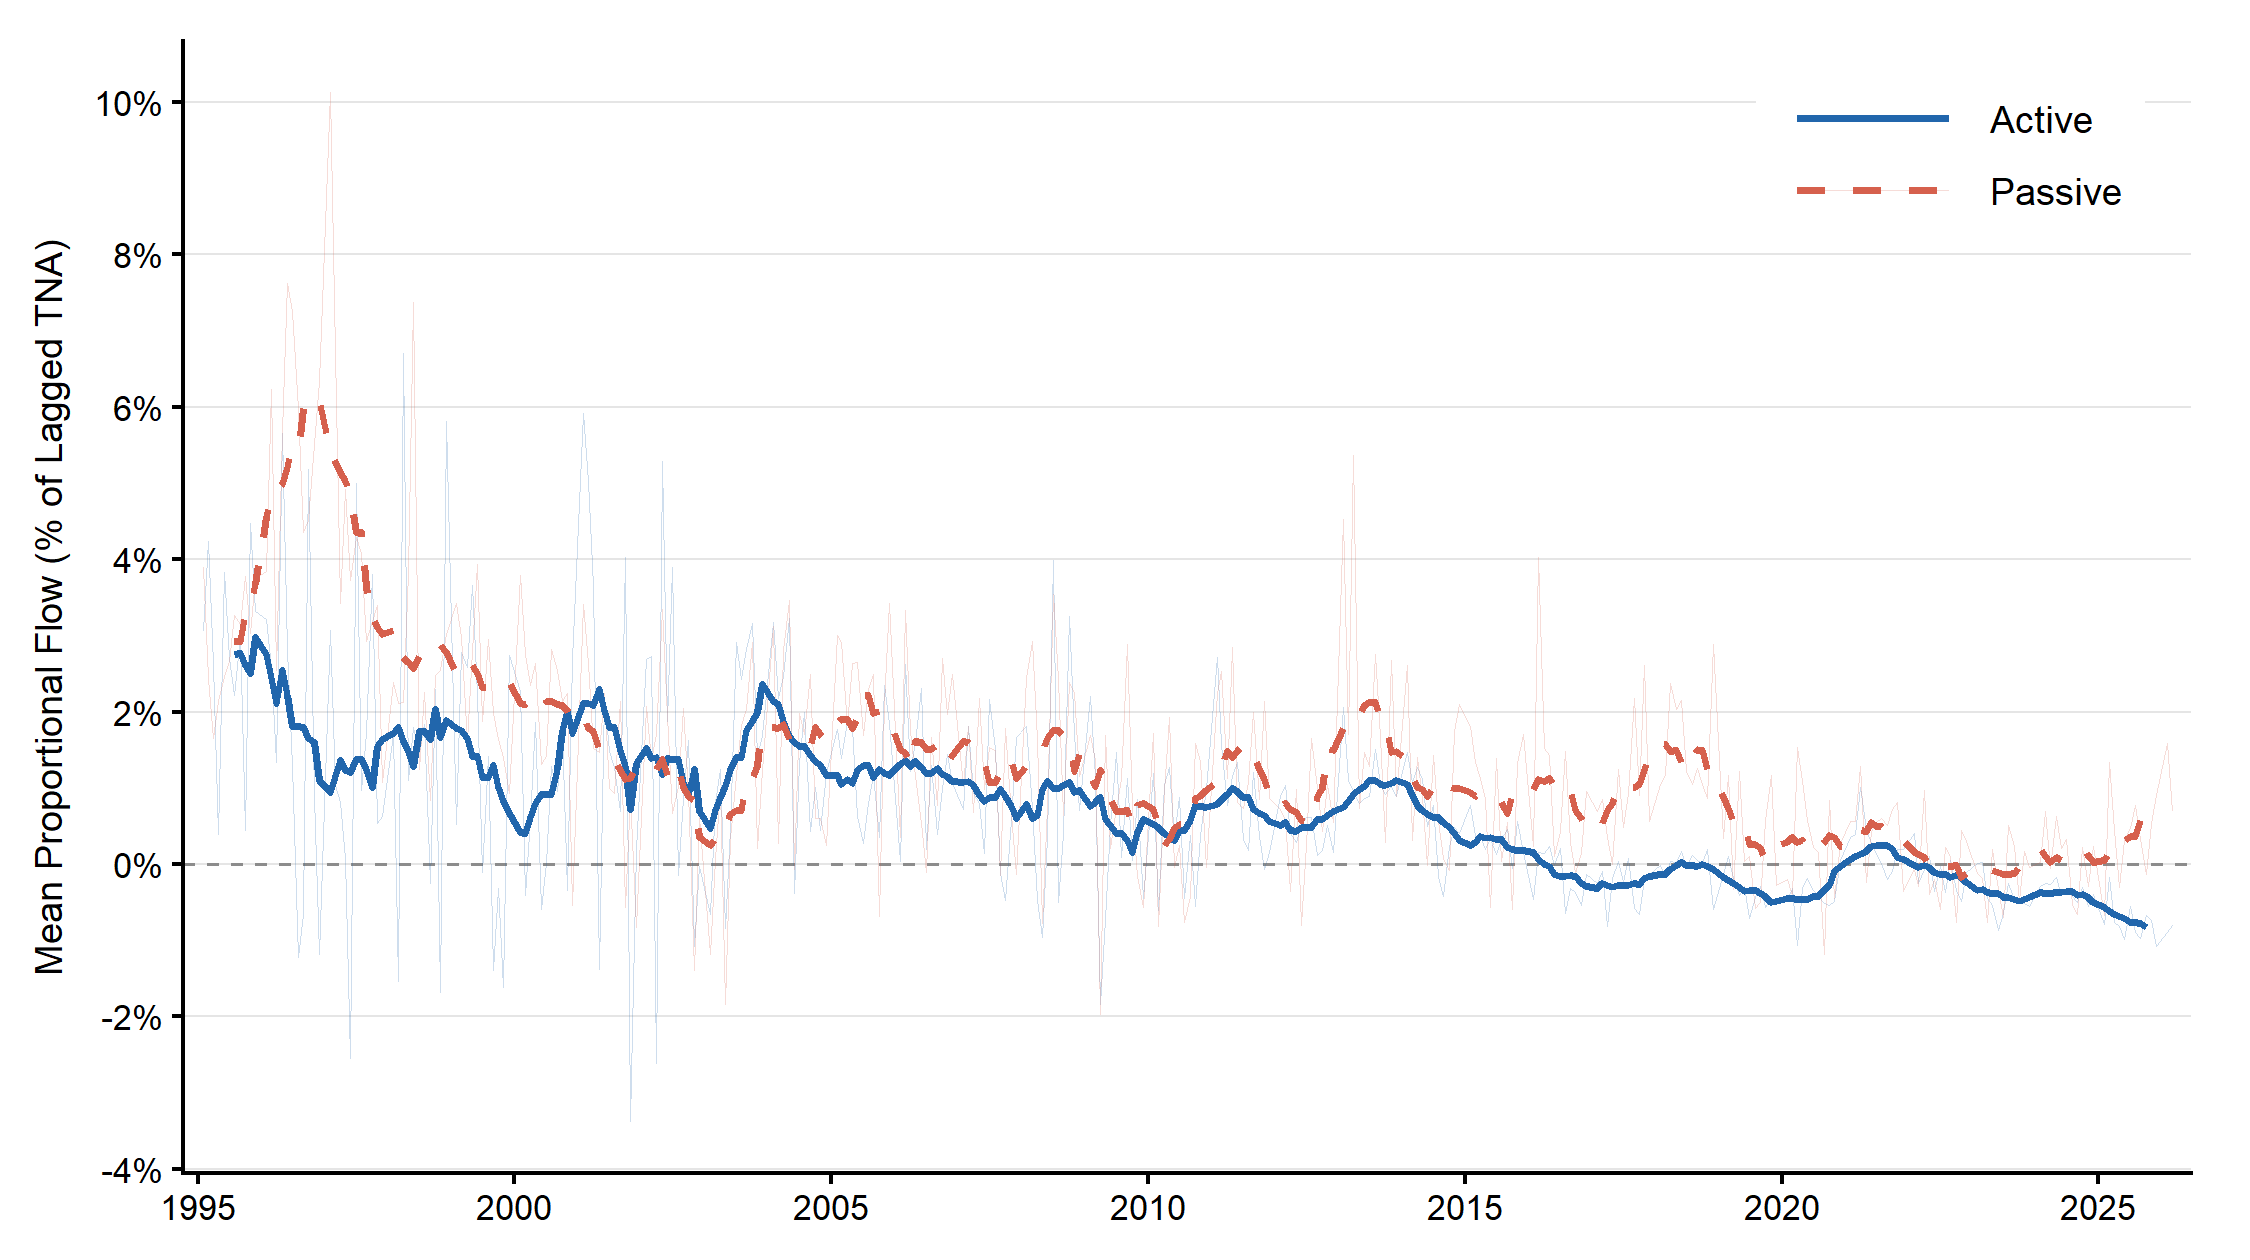
\includegraphics[width=\textwidth]{tables/fig_fund_flows.png}
  \caption[Average monthly proportional fund flows: active vs.\ passive]{%
    Average monthly proportional fund flows for actively and passively
    managed domestic-equity mutual funds in the U.S.\ universe. For each
    group, the bold line is the 12-month centred rolling mean of the
    cross-sectional equal-weighted average of $\text{Flow}_{i,t}$, the
    \textcite{SirriTufano1998} proportional flow defined as
    $\text{Flow}_{i,t} = (\text{TNA}_{i,t} - \text{TNA}_{i,t-1}
    (1+R_{i,t})) / \text{TNA}_{i,t-1}$, scaled by lagged TNA and
    winsorised at the 1st and 99th percentiles, with December
    observations excluded. The faint line is the raw monthly
    cross-sectional mean. Active funds are shown in dark blue (solid),
    passive funds in red (dashed). Unknown-classified funds are
    excluded.}
  \label{fig:fund_flows}
\end{figure}

Figure~\ref{fig:fund_flows} plots the cross-sectional equal-weighted
average of monthly proportional flows. Average flows into passive funds
exceed those into active funds in almost every year of the sample. Active
flows decline from roughly 2--3\% of assets per month in the mid-1990s to
about 1\% in the mid-2000s, recover briefly after 2010, turn negative
around 2016, and remain negative thereafter, reaching about $-0.8\%$ per
month at the end of the sample. The post-2015 net-outflow regime is
consistent with the secular shift of retail capital from active to
passive vehicles during the 2010s \parencite{IndexEffect2018}. It is
notable that the turn to sustained outflows comes several years after the
deterioration in active performance documented in
Section~\ref{sec:subperiod}: capital leaves slowly.

\section{Aggregate fund performance}
\label{sec:aggregate_performance}

\noindent Table~\ref{tab:perf_aggregate} reports the central performance
result of the dissertation. Before fees, the aggregate active portfolio
earns a Carhart alpha that is economically small and statistically
indistinguishable from zero: $+0.223\%$ per annum equal-weighted
($t = 0.47$) and $+0.027\%$ value-weighted ($t = 0.07$). Active managers,
as a group, neither add nor destroy value relative to the four factors
before they are paid.

\begin{table}[!htbp]
\centering
\sbox{\tabletempbox}{%
\footnotesize
\begin{tabular}[t]{lrrrrrr}
\toprule
\multicolumn{3}{c}{ } & \multicolumn{2}{c}{Gross Alpha} & \multicolumn{2}{c}{Net Alpha} \\
\cmidrule(l{3pt}r{3pt}){4-5} \cmidrule(l{3pt}r{3pt}){6-7}
Group & $N$ & $T$ & EW & VW & EW & VW\\
\midrule
Active & 1,952 & 373 & 0.223 & 0.027 & -0.823$^{*}$ & -0.658\\
t(coef) &  &  & (0.47) & (0.07) & (-1.75) & (-1.62)\\
Passive & 269 & 373 & -0.262 & 0.049 & -0.693$^{**}$ & -0.057\\
t(coef) &  &  & (-0.96) & (0.29) & (-2.54) & (-0.34)\\
Unknown & 660 & 373 & -2.097$^{***}$ & -2.647$^{**}$ & -3.406$^{***}$ & -3.746$^{***}$\\
t(coef) &  &  & (-2.84) & (-2.13) & (-4.63) & (-3.01)\\
\midrule
Active + Passive & 2,221 & 373 & 0.171 & 0.030 & -0.813$^{*}$ & -0.532\\
t(coef) &  &  & (0.39) & (0.09) & (-1.83) & (-1.53)\\
Full Sample & 2,881 & 373 & -0.115 & 0.022 & -1.139$^{***}$ & -0.542\\
t(coef) &  &  & (-0.27) & (0.06) & (-2.70) & (-1.58)\\
\bottomrule
\end{tabular}%
}
\setlength{\tabletempwidth}{\wd\tabletempbox}
\ifdim\tabletempwidth>\linewidth\setlength{\tabletempwidth}{\linewidth}\fi
\begin{minipage}{\tabletempwidth}
\captionsetup{width=\linewidth}
\caption{\label{tab:perf_aggregate}Aggregate Portfolio Alpha by Group (\%, Annualised)}
\ifdim\wd\tabletempbox>\linewidth
  \resizebox{\linewidth}{!}{\usebox{\tabletempbox}}
\else
  \usebox{\tabletempbox}
\fi
\par\medskip
\begin{singlespace}\footnotesize\noindent
Annualised \textcite{Carhart1997} four-factor alpha (\%) from regressing the monthly aggregate portfolio return of each group on the market, size, value, and momentum factors, following \textcite{FamaFrench2010}. EW: equal-weighted portfolio (each fund alive in month $t$ contributes $1/N_t$). VW: value-weighted portfolio with lagged TNA weights $w_{i,t-1} = \text{TNA}_{i,t-1} / \sum_j \text{TNA}_{j,t-1}$. Net returns are the funds' NAV-based total returns (net of expenses); gross returns add back one-twelfth of the static annual expense ratio each month, following \textcite{FamaFrench2010}. Newey-West $t$-statistics (6-month lag) in parentheses below each alpha; $^{*}$, $^{**}$, $^{***}$: significant at 10\%, 5\%, 1\%. $N$: unique funds contributing to the portfolio series; $T$: number of monthly observations in the regression. The Active + Passive row aggregates only the two classified groups. Sample: Incubation-corrected panel (Evans 2010), no date cap; performance-comparison subsample per flagged\_funds.xlsx.
\end{singlespace}
\end{minipage}
\end{table}



Net of fees, the aggregate equal-weighted alpha of active funds is
$-0.823\%$ per annum ($t = -1.75$, significant at 10\%) and the
value-weighted alpha is $-0.658\%$ per annum ($t = -1.62$, not significant
at conventional levels). The difference between the gross and net
estimates is, by construction, the average expense ratio; the net
shortfall is therefore almost exactly the cost of active management.
These magnitudes are close to those of \textcite{FamaFrench2010} for
1984--2006, who report four-factor gross alphas of $0.39\%$ (EW) and
$-0.05\%$ (VW) per annum and net alphas between $-0.81\%$ and $-1.00\%$
per annum, and who conclude that the high costs of active management show
up intact as lower returns to investors. The present sample extends that
conclusion by almost two decades.

Two features of the result merit emphasis. First, the gap between the
equal-weighted and value-weighted net alphas is small (17 basis points)
and statistically unimportant: the aggregate shortfall is not driven by
the many small funds that dominate the equal-weighted average, but is
shared by the representative dollar. Second, the precision of the
estimates is limited. Over 31 years of monthly data, an annual net alpha
of $-0.7\%$ to $-0.8\%$ is only marginally distinguishable from zero.
The aggregate evidence alone therefore cannot discriminate sharply
between the \textcite{BerkGreen2004} prediction of a zero net alpha and
the equilibrium-accounting prediction of a net alpha equal to minus
costs; the cross-sectional and sub-period evidence below is more
informative.

Passive funds provide a useful benchmark. Their gross alphas are close to
zero ($-0.262\%$ EW, $+0.049\%$ VW), and their equal-weighted net alpha is
$-0.693\%$ ($t = -2.54$), driven by the many small, relatively expensive
index funds; the value-weighted passive net alpha is only $-0.057\%$. The
value-weighted comparison is the economically relevant one for an
investor choosing between the two industries: the representative active
dollar earns about 60 basis points per annum less than the representative
passive dollar, which is roughly the fee differential between them.

The unknown-classified group performs materially worse than either
active or passive funds: an equal-weighted net alpha of $-3.406\%$ per
annum and a value-weighted net alpha of $-3.746\%$, both significant at
1\%. The group consists of share classes for which the active-management
flag is not populated; inspection of fund names indicates that it is
dominated by small, short-lived funds, many of which were liquidated
early in the sample. The group is excluded from all regression analyses
but is reported for completeness.

\begin{figure}[H]
  \centering
  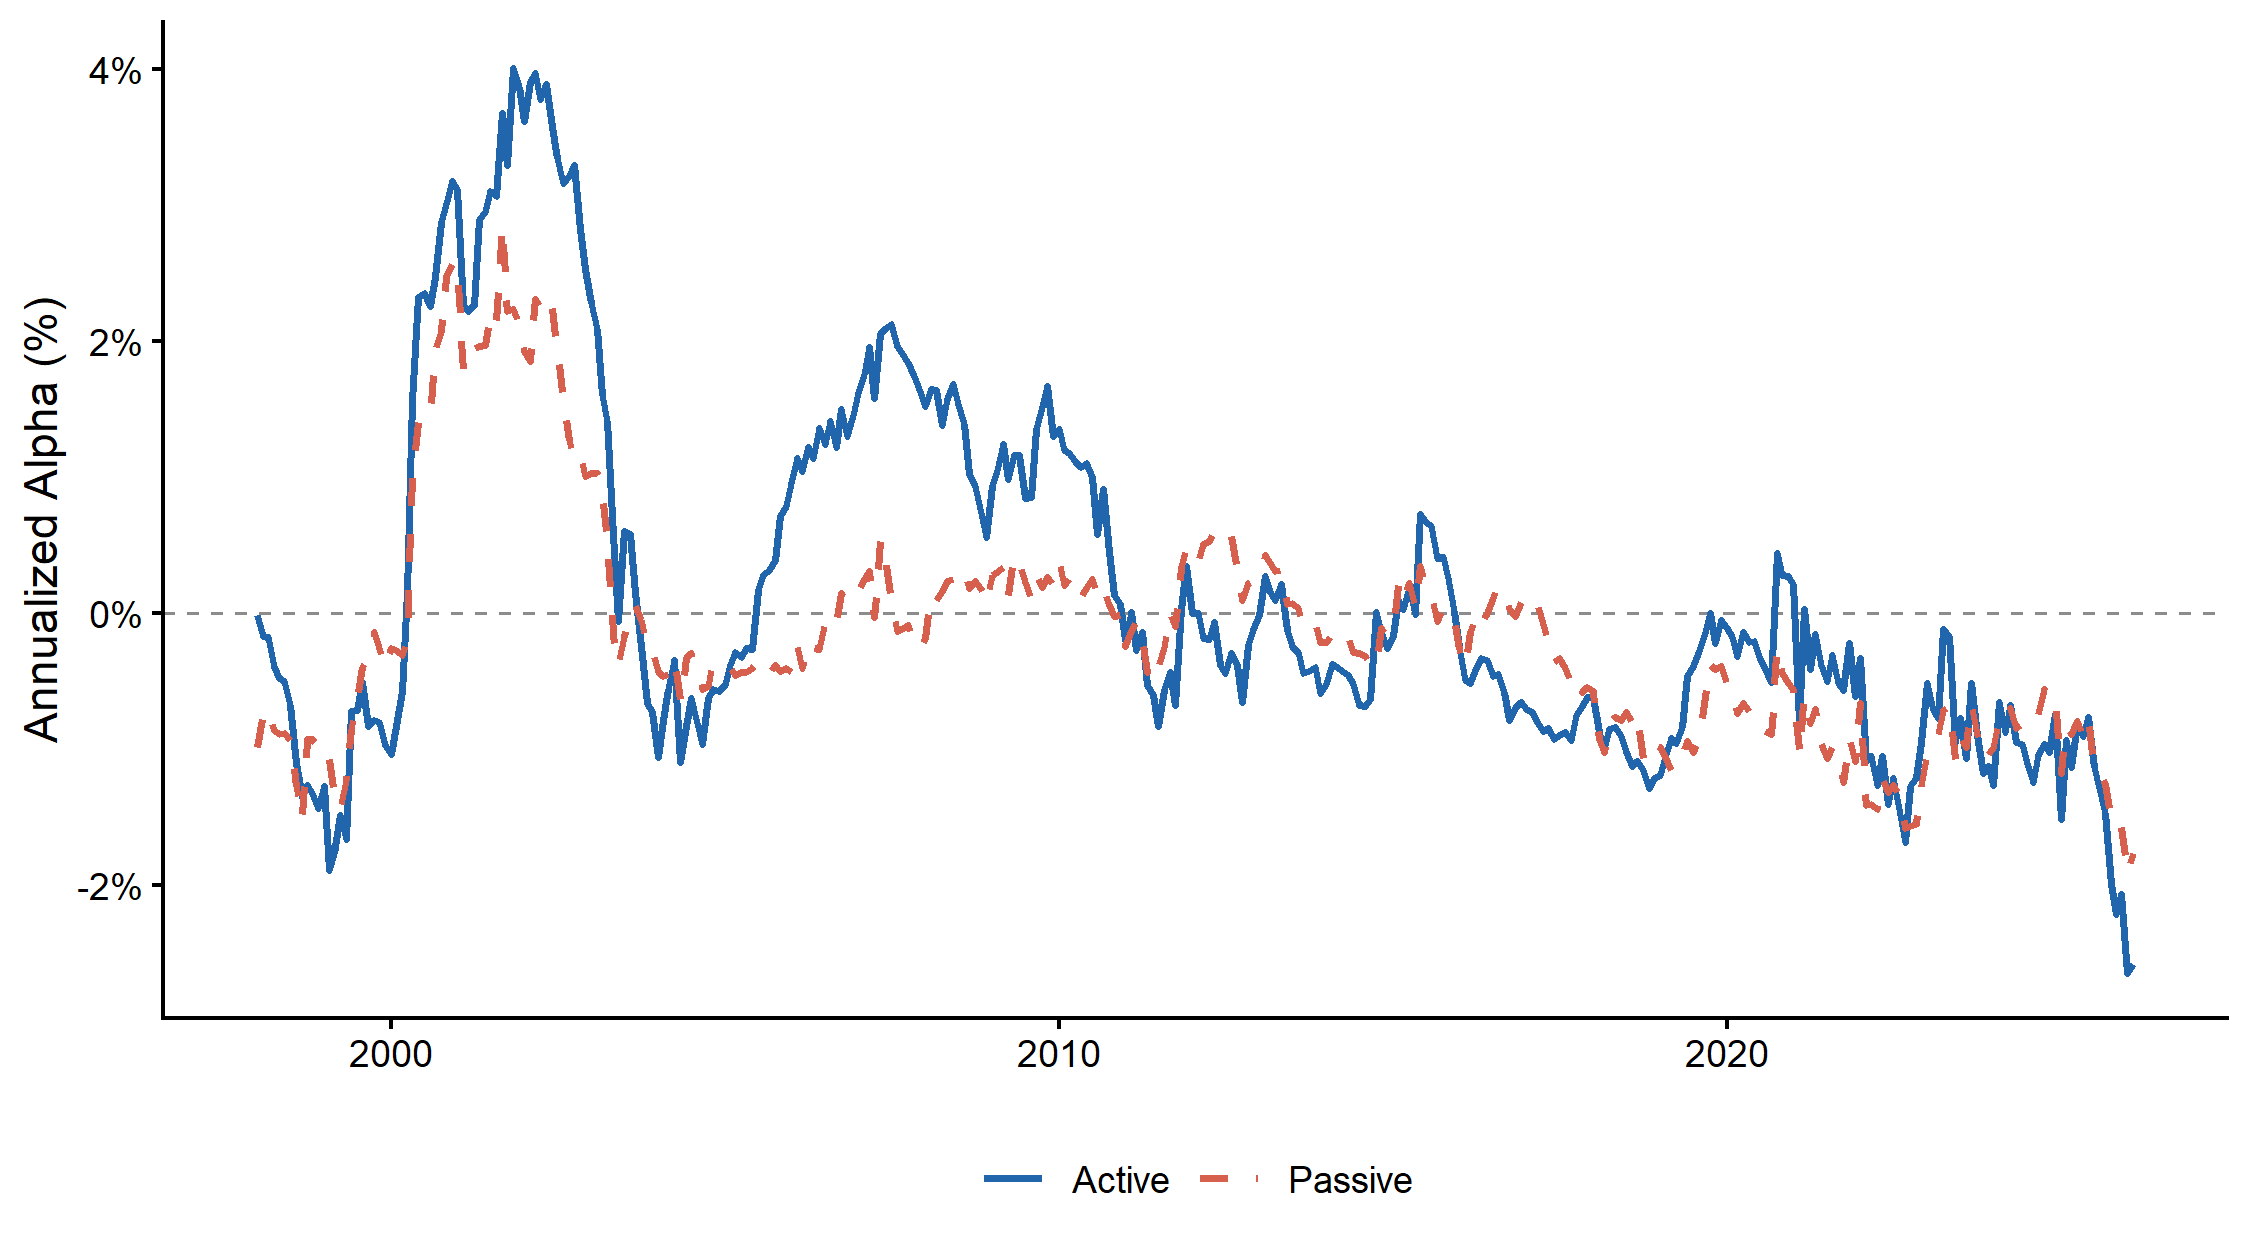
\includegraphics[width=\textwidth]{tables/fig_rolling_alphas.png}
  \caption[Rolling aggregate gross alpha: active vs.\ passive]{%
    Rolling aggregate gross alpha for actively and passively managed
    domestic-equity mutual funds, estimated month by month following
    \textcite{FamaFrench2010}. For each group $g$ and each month $t$,
    the aggregate gross return $R^{g}_t$ is the equal-weighted average
    return of all funds alive in month $t$. The series plotted is the
    intercept (annualised by multiplication by twelve) of a
    \textcite{Carhart1997} four-factor regression of the monthly
    aggregate excess return $R^{g}_t - R^{f}_t$ on the market, size,
    value, and momentum factors over a 36-month trailing window. This
    is a portfolio-level regression rather than a cross-sectional
    average of per-fund rolling alphas; rolling regression already
    smooths the series so no additional moving-average smoothing is
    applied. Break dates estimated on the cross-sectional mean of
    per-fund rolling alphas are reported in Appendix~\ref{app:subperiod}.
    Sample: Incubation-corrected panel (Evans 2010), no date cap,
    performance-comparison subsample per flagged\_funds.xlsx;
    Unknown-classified funds excluded.}
  \label{fig:rolling_alphas}
\end{figure}

Figure~\ref{fig:rolling_alphas} plots the rolling 36-month gross alpha of
the equal-weighted active and passive portfolios. The active series is
far from stable. It is negative in the late 1990s, rises to about 4\% per
annum in the 36-month windows ending in 2001--2002, which contain the
aftermath of the technology-stock collapse, falls back below zero by
2004, and is positive again, at 1--2\% per annum, in the windows ending
between 2006 and 2010. From 2011 onwards the series fluctuates around or
below zero and drifts downward, ending near $-2.5\%$ per annum in the
window ending in early 2026. The passive series tracks the active series
at a lower amplitude, which indicates that part of the time variation
reflects factor-model misspecification common to all equity funds rather
than managerial skill. The formal break test and the sub-period analysis
built on it are summarised in Section~\ref{sec:subperiod}.

\section{Luck versus skill: Bootstrap analysis}
\label{sec:bootstrap_results}

\noindent Table~\ref{tab:bootstrap_tails} compares percentiles of the
cross-section of actual $t(\hat{\alpha})$ estimates for the 1{,}800 active
funds with at least 24 monthly observations against the same percentiles
in $10{,}000$ bootstrap simulations in which every fund's true gross
alpha is zero. No percentile of the actual distribution is
distinguishable from its zero-skill counterpart. In the left tail the
actual $t$-statistics are somewhat more negative than the simulated ones
($-3.15$ against $-2.61$ at the 1st percentile, $-2.13$ against $-1.75$
at the 5th, $-1.67$ against $-1.34$ at the 10th), but simulated
percentiles at least as extreme occur in 7.2\%, 11.2\% and 13.4\% of the
iterations respectively. In the right tail the actual and simulated
percentiles are almost identical ($1.36$ against $1.36$ at the 90th
percentile, $2.63$ against $2.65$ at the 99th).

\begin{table}[!htbp]
\centering
\sbox{\tabletempbox}{%
\footnotesize
\begin{tabular}[t]{rrrr>{\raggedright\arraybackslash}p{15em}}
\toprule
Percentile & Actual $t(\hat{\alpha})$ & Simulated Mean & Prob.\ Luck & Interpretation\\
\midrule
1 & -3.154 & -2.606 & 7.2\% & Consistent with zero skill\\
5 & -2.128 & -1.745 & 11.2\% & Consistent with zero skill\\
10 & -1.669 & -1.339 & 13.4\% & Consistent with zero skill\\
50 & -0.188 & 0.006 & 24.9\% & Consistent with zero skill\\
90 & 1.359 & 1.359 & 53.3\% & Consistent with zero skill\\
95 & 1.740 & 1.770 & 50.0\% & Consistent with zero skill\\
99 & 2.633 & 2.645 & 52.6\% & Consistent with zero skill\\
\bottomrule
\end{tabular}%
}
\setlength{\tabletempwidth}{\wd\tabletempbox}
\ifdim\tabletempwidth>\linewidth\setlength{\tabletempwidth}{\linewidth}\fi
\begin{minipage}{\tabletempwidth}
\captionsetup{width=\linewidth}
\caption{\label{tab:bootstrap_tails}Fama--French (2010) Bootstrap: Actual vs.\ Simulated $t(\hat{\alpha})$ Percentiles}
\ifdim\wd\tabletempbox>\linewidth
  \resizebox{\linewidth}{!}{\usebox{\tabletempbox}}
\else
  \usebox{\tabletempbox}
\fi
\par\medskip
\begin{singlespace}\footnotesize\noindent
Bootstrap procedure follows \textcite{FamaFrench2010}. Sample: actively managed funds, Incubation-corrected (Evans 2010) panel (no date cap), performance-comparison subsample per flagged\_funds.xlsx, minimum 24 monthly observations ($N = 1800$ funds). For each fund, estimated monthly alpha is subtracted from the excess return series to construct a zero-alpha null return. In each of $B = 10{,}000$ bootstrap iterations, calendar months are resampled with replacement and kept in the order drawn, the same draw applying to all funds, preserving cross-sectional factor return dependence. The \textcite{Carhart1997} four-factor model is re-estimated on each resampled series. \textit{Actual} $t(\hat{\alpha})$: percentile of the empirical $t$-statistic distribution across active funds. \textit{Simulated Mean}: average of that percentile across all iterations. \textit{Prob.\ Luck}: fraction of iterations in which the simulated percentile falls below the actual value; values below 5\% (above 95\%) indicate that the actual percentile is worse (better) than zero-alpha luck would produce; 0.0\% means no iteration and $<$0.1\% means 1 to 4 of 10,000 iterations. Newey-West standard errors with a 6-month lag are used throughout.
\end{singlespace}
\end{minipage}
\end{table}



The full-period cross-section of gross alphas is therefore consistent
with a world in which no active manager has true alpha, before fees,
relative to the Carhart model. This is a weaker result than
\textcite{FamaFrench2010} report for 1984--2006, where gross returns
show evidence of both inferior and superior true alpha in the extreme
tails. Two qualifications prevent a stronger reading. First, the
bootstrap tests the cross-section as a whole and has limited power
against a small skilled or unskilled minority; the false-discovery
decomposition in the next section addresses this directly. Second, the
result depends on the factor model and on the period. Under the
\textcite{FamaFrench2015} five-factor model augmented with momentum, the
left tail is worse than luck at the 1st, 5th and 10th percentiles
(Appendix~\ref{app:robustness}), and within the post-2010 sub-period it
is worse than luck under the Carhart model as well
(Appendix~\ref{app:subperiod}).

\section{False discovery decomposition}
\label{sec:fdr_results}

\noindent Table~\ref{tab:pi0_estimate} reports the \textcite{Storey2002}
estimate of the population proportion of zero-alpha active funds
(Equation~\ref{eq:storey}). On the incubation-corrected panel,
$\hat{\pi}_0 = 87.1\%$ at the standard tuning parameter $\lambda = 0.5$:
roughly seven in eight active funds have a true gross alpha that is
estimated to be zero. The estimate is conservative in the
\textcite{BarrasScailletWermers2010} sense, overstating the zero-alpha
proportion when non-zero-alpha funds have large $p$-values.

\begin{table}[!htbp]
\centering
\sbox{\tabletempbox}{%
\footnotesize
\begin{tabular}[t]{>{\raggedright\arraybackslash}p{16em}rrr>{\raggedright\arraybackslash}p{14em}}
\toprule
Metric & Estimate & $N$ & $\lambda$ & Interpretation\\
\midrule
$\hat{\pi}_0$: Proportion of True Zero-Alpha Active Funds & 87.1\% & 1,800 & 0.5 & Heterogeneous skill; majority zero-alpha\\
\bottomrule
\end{tabular}%
}
\setlength{\tabletempwidth}{\wd\tabletempbox}
\ifdim\tabletempwidth>\linewidth\setlength{\tabletempwidth}{\linewidth}\fi
\begin{minipage}{\tabletempwidth}
\captionsetup{width=\linewidth}
\caption{\label{tab:pi0_estimate}Aggregate Skill Estimate: Proportion of True Zero-Alpha Active Funds}
\ifdim\wd\tabletempbox>\linewidth
  \resizebox{\linewidth}{!}{\usebox{\tabletempbox}}
\else
  \usebox{\tabletempbox}
\fi
\par\medskip
\begin{singlespace}\footnotesize\noindent
The proportion of true zero-alpha funds ($\hat{\pi}_0$) is estimated following \textcite{Storey2002} and \textcite{BarrasScailletWermers2010}, using p-values from Newey-West $t$-tests on full-period \textcite{Carhart1997} four-factor alphas. The estimator is $\hat{\pi}_0 = |\{p_i > \lambda\}| \,/\, [N(1-\lambda)]$, where $\lambda = 0.5$ is the standard tuning parameter following \textcite{Storey2002}. Funds with p-values exceeding $\lambda$ are unlikely to have non-zero true alpha; the density of p-values in $(\lambda, 1]$ provides a conservative estimate of the zero-alpha proportion, bounded above at 1. Sample: actively managed funds ($N = 1,800$), Incubation-corrected (Evans 2010) panel, no date cap; performance-comparison subsample per flagged\_funds.xlsx. Passive and Unknown-classified funds are excluded. The four-way decomposition of skilled, unskilled, and lucky fund proportions implied by this estimate is reported in Table~\ref{tab:bsw_decomposition}.
\end{singlespace}
\end{minipage}
\end{table}



\begin{figure}[H]
  \centering
  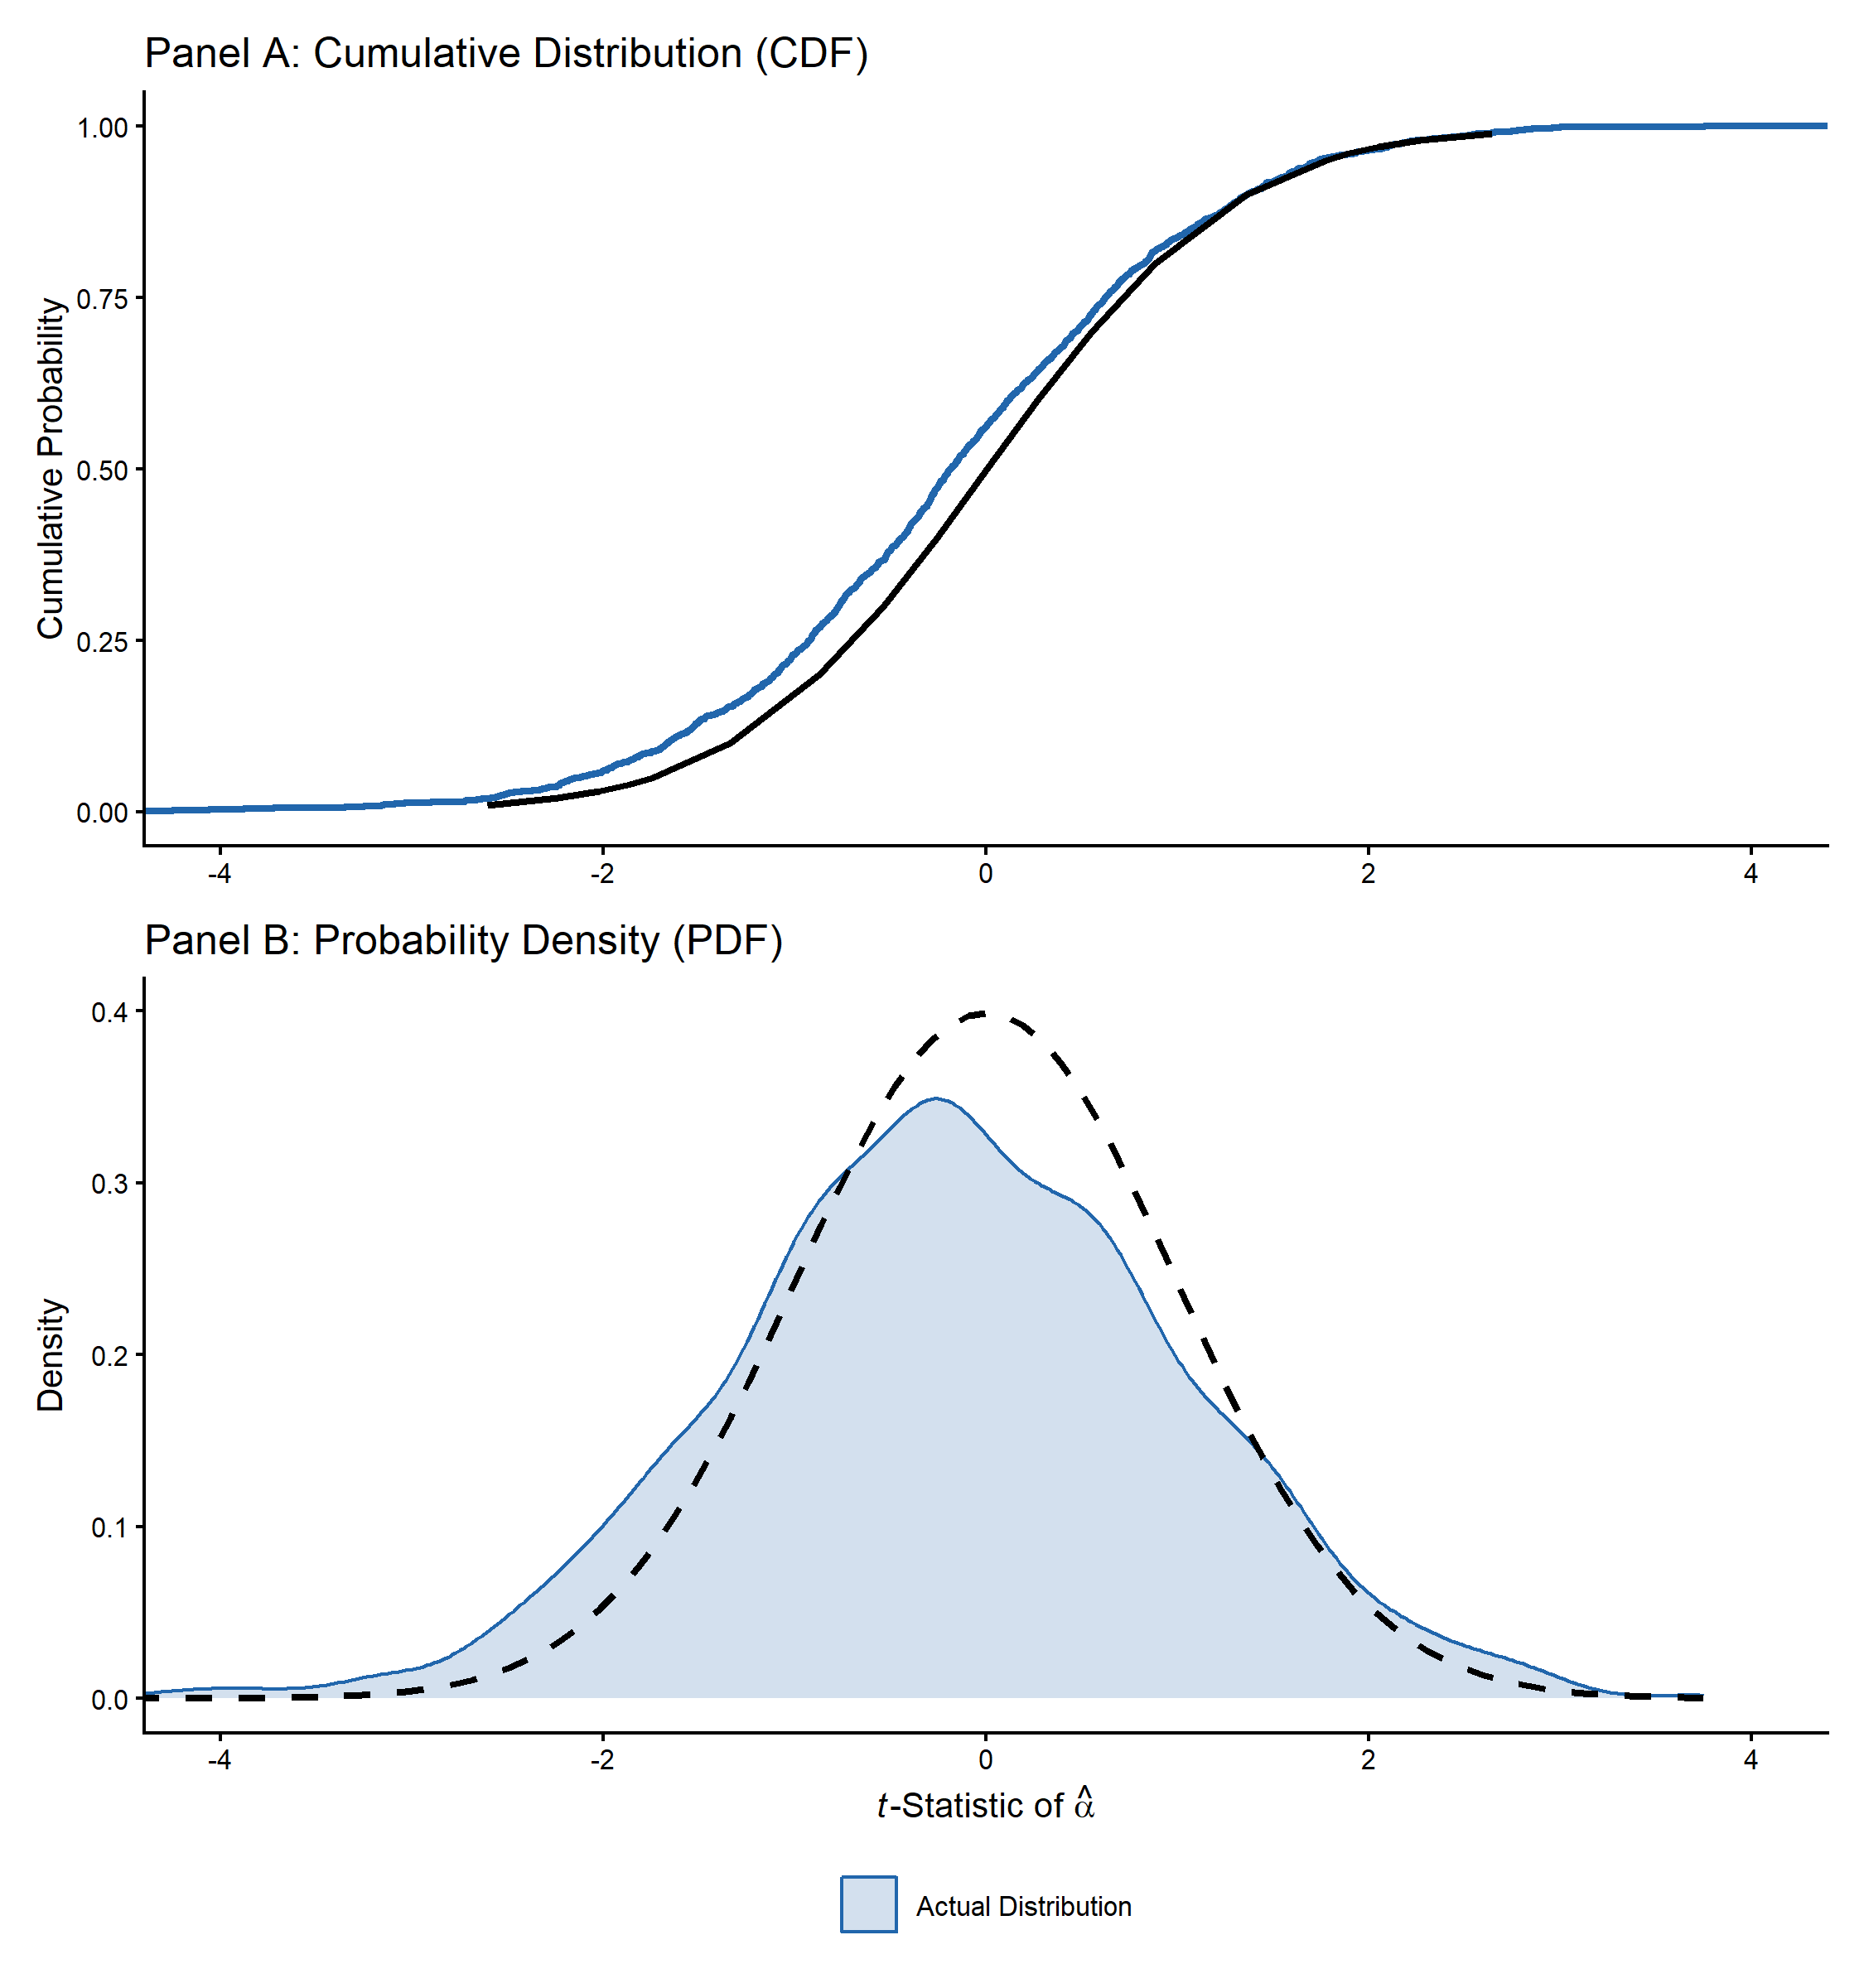
\includegraphics[width=\textwidth]{tables/fig_luck_vs_skill_combined.png}
  \caption[CDF and PDF of empirical vs.\ simulated alpha $t$-statistics]{%
    Cross-sectional distribution of \textcite{Carhart1997} four-factor
    alpha $t$-statistics for actively managed funds, with simulated
    zero-skill comparison. Panel A: empirical cumulative
    distribution function (CDF) of active-fund $t(\hat{\alpha})$ (solid
    blue) versus the \textcite{FamaFrench2010} bootstrap-derived
    zero-skill CDF (solid black, dashed line type), constructed by
    resampling calendar months with replacement and re-estimating each
    fund's $t(\hat{\alpha})$ on the resampled sample after subtracting
    its actual full-period alpha to impose the zero-skill null.
    Panel B: kernel density of the empirical $t$-statistic
    distribution (shaded blue) against the theoretical $N(0,1)$
    reference (dashed black). The $N(0,1)$ reference is included as a
    visual benchmark for the no-skill hypothesis under normality; the
    bootstrap null in Panel A is the inferentially appropriate
    comparison and accounts for cross-sectional dependence, fat tails,
    and finite-sample estimation error. Percentile-level bootstrap
    comparisons are reported in Table~\ref{tab:bootstrap_tails}.
    Sample: actively managed funds in the Incubation-corrected
    (Evans 2010) panel, performance-comparison subsample per
    flagged\_funds.xlsx, with at least 24 monthly observations.}
  \label{fig:luck_vs_skill}
\end{figure}

Figure~\ref{fig:luck_vs_skill} plots the empirical and
bootstrap-simulated distributions of active-fund $t$-statistics. The
empirical distribution is shifted slightly to the left of the bootstrap
null --- the median actual $t$-statistic is $-0.19$ against a simulated
median of $0.01$ --- and is somewhat more dispersed in the left tail, but
the two distributions are close over most of the support. The visual
evidence matches the percentile-by-percentile tests: a mild leftward tilt
that the bootstrap does not distinguish from luck.

\begin{table}[!htbp]
\centering
\sbox{\tabletempbox}{%
\footnotesize
\begin{tabular}[t]{rrrrrr}
\toprule
\multicolumn{1}{c}{ } & \multicolumn{2}{c}{Observed Tails} & \multicolumn{1}{c}{False Disc.} & \multicolumn{2}{c}{True Proportions} \\
\cmidrule(l{3pt}r{3pt}){2-3} \cmidrule(l{3pt}r{3pt}){4-4} \cmidrule(l{3pt}r{3pt}){5-6}
$\gamma$ & $S^-_\gamma$ & $S^+_\gamma$ & $F_\gamma$ & $T^-_\gamma$ & $T^+_\gamma$\\
\midrule
5\% & 5.9 & 3.6 & 2.2 & 3.8 & 1.4\\
10\% & 10.1 & 6.1 & 4.4 & 5.7 & 1.8\\
15\% & 14.1 & 8.8 & 6.5 & 7.5 & 2.2\\
20\% & 16.1 & 11.4 & 8.7 & 7.4 & 2.7\\
25\% & 18.8 & 13.4 & 10.9 & 7.9 & 2.6\\
30\% & 21.9 & 15.4 & 13.1 & 8.8 & 2.4\\
35\% & 24.5 & 17.2 & 15.2 & 9.3 & 2.0\\
40\% & 27.6 & 19.4 & 17.4 & 10.2 & 2.0\\
45\% & 30.6 & 21.1 & 19.6 & 11.0 & 1.5\\
50\% & 33.1 & 23.4 & 21.8 & 11.3 & 1.6\\
\bottomrule
\end{tabular}%
}
\setlength{\tabletempwidth}{\wd\tabletempbox}
\ifdim\tabletempwidth>\linewidth\setlength{\tabletempwidth}{\linewidth}\fi
\begin{minipage}{\tabletempwidth}
\captionsetup{width=\linewidth}
\caption{\label{tab:bsw_decomposition}BSW (2010) Four-Way Decomposition: Proportions of Skilled, Unskilled, and Lucky Funds (\%)}
\ifdim\wd\tabletempbox>\linewidth
  \resizebox{\linewidth}{!}{\usebox{\tabletempbox}}
\else
  \usebox{\tabletempbox}
\fi
\par\medskip
\begin{singlespace}\footnotesize\noindent
Decomposition follows \textcite{BarrasScailletWermers2010}, Section~II.B and Table~III. $S^-_\gamma$ ($S^+_\gamma$): observed fraction of active funds with significantly negative (positive) Newey-West $t(\hat{\alpha})$ at two-sided significance level $\gamma$, using full-period \textcite{Carhart1997} four-factor alphas and the same Student-$t$ $p$-values as $\hat{\pi}_0$. $F_\gamma = \hat{\pi}_0 \cdot \gamma/2$: expected proportion of false discoveries per tail arising from zero-alpha funds, where $\hat{\pi}_0 = 87.1\%$ is the \textcite{Storey2002} estimate at $\lambda = 0.5$ (see Table~\ref{tab:pi0_estimate}). $T^-_\gamma = S^-_\gamma - F_\gamma$: genuinely unskilled funds (significant negative alpha net of false discoveries). $T^+_\gamma = S^+_\gamma - F_\gamma$: genuinely skilled funds (significant positive alpha net of false discoveries). The row at $\gamma^* = 0.45$ gives the population estimates $\hat{\pi}^-_A$ and $\hat{\pi}^+_A$ (\citealt{BarrasScailletWermers2010}, eq.~8, who take them at a sufficiently high $\gamma^*$ and report that pre-set values of 0.35 or 0.45 match their MSE-based choice). Negative $T^+_\gamma$ entries indicate right-tail significance does not exceed the false-discovery rate at that threshold. The Storey estimator is conservative: it overestimates $\hat{\pi}_0$ when truly skilled funds exist, so $T^+_\gamma$ values are lower bounds. All quantities are percentages of the active-fund universe. Sample: $N = 1,800$ actively managed funds, Incubation-corrected (Evans 2010) panel, no date cap; performance-comparison subsample per flagged\_funds.xlsx; Passive and Unknown funds excluded.
\end{singlespace}
\end{minipage}
\end{table}



Table~\ref{tab:bsw_decomposition} reports the
\textcite{BarrasScailletWermers2010} four-way decomposition. At the
threshold $\gamma^* = 0.45$, at which the population proportions are
read, the observed left-tail significance fraction is
$S^-_{\gamma^*} = 30.6\%$ and the right-tail fraction is
$S^+_{\gamma^*} = 21.1\%$. The expected false-discovery fraction per tail
is $F_{\gamma^*} = \hat{\pi}_0 \cdot \gamma^* / 2 = 0.871 \cdot 0.225 =
19.6\%$. The genuinely unskilled mass is therefore
$\hat{\pi}^-_A = 30.6\% - 19.6\% = 11.0\%$, and the genuinely skilled mass
is $\hat{\pi}^+_A = 21.1\% - 19.6\% = 1.5\%$.

The decomposition sharpens the bootstrap result. About one active fund in
nine has a negative true gross alpha, and only about one in seventy has a
positive one. The unskilled mass is positive at every threshold in the
grid, rising from 3.8\% at $\gamma = 0.05$ to 11.3\% at $\gamma = 0.50$;
the skilled mass stays between 1.4\% and 2.7\%. Reading the population
proportions at $\gamma = 0.20$ instead would give 7.4\% unskilled and 2.7\% skilled funds; the
qualitative conclusion is unchanged, but the low threshold understates
the population proportions for the reason given in
Section~\ref{sec:fdr_methodology}. The skilled share of 1.5\% compares
with 0.6\% at the end of the \textcite{BarrasScailletWermers2010} sample,
and the unskilled share of 11.0\% with their 24.0\%. Because the present
decomposition is applied to gross rather than net alphas, a fund counted
as unskilled here fails to match the factor benchmark even before its
fees are deducted. The decomposition does not imply that managerial skill
is absent in the \textcite{BerkVanBinsbergen2015} dollar-value sense; it
implies that, over the full sample, the population mass of managers whose
alpha is detectably positive is small. Section~\ref{sec:subperiod} shows
that this full-sample average conceals a substantial skilled minority
before 2010 and none afterwards.

\section{Portfolio sorts: Size, momentum, and fee}
\label{sec:portfolio_sorts}

\noindent Tables~\ref{tab:port_characteristics} through
\ref{tab:port_fee_alpha} report characteristics and gross alphas of
quintile portfolios sorted on three fund characteristics: log lagged TNA
(size), the cumulative 11-month net return ending in month $t-2$,
skipping $t-1$ (momentum, following \textcite{JegadeeshTitman1993}), and
the static annual expense ratio (fee). Quintiles are formed monthly within
group (active or passive), and equal-weighted and value-weighted portfolio
gross returns are regressed on the CAPM, Fama--French three-factor and
Carhart four-factor models with Newey--West standard errors at a
six-month lag. Because the expense ratio is an end-of-sample value, the
fee sort uses information that was not available in real time and should
be read as descriptive.


{\setlength{\tabcolsep}{3pt}\setlength{\LTpost}{0pt}\footnotesize
\captionsetup{font=normalsize}\begin{longtable}[t]{lrrrrrrr}
\caption{\label{tab:port_characteristics}Portfolio Characteristics by Sort Variable and Quintile}\\
\toprule
$Q$ & $N_{\text{avg}}$ & TNA & ER & Turn. & EW Gross & VW Gross & EW Sharpe\\
\midrule
\endfirsthead
\caption[]{Portfolio Characteristics by Sort Variable and Quintile \textit{(continued)}}\\
\toprule
$Q$ & $N_{\text{avg}}$ & TNA & ER & Turn. & EW Gross & VW Gross & EW Sharpe\\
\midrule
\endhead

\endfoot
\bottomrule
\endlastfoot
\addlinespace[0.3em]
\multicolumn{8}{l}{Panel A: Size --- Active}\\
\hspace{1em}Q1 & 183 & 84 & 1.26 & 67.3 & 1.003 & 1.015 & 0.62\\
\hspace{1em}Q2 & 183 & 308 & 1.02 & 54.4 & 1.017 & 1.021 & 0.62\\
\hspace{1em}Q3 & 183 & 764 & 0.95 & 52.2 & 1.034 & 1.030 & 0.63\\
\hspace{1em}Q4 & 183 & 1,995 & 0.90 & 52.1 & 1.007 & 0.993 & 0.60\\
\hspace{1em}Q5 & 183 & 11,130 & 0.73 & 39.3 & 0.964 & 0.973 & 0.59\\
\addlinespace[0.3em]
\hline
\multicolumn{8}{l}{Panel B: Size --- Passive}\\
\hspace{1em}Q1 & 22 & 141 & 0.84 & 221.9 & 1.118 & 1.088 & 0.63\\
\hspace{1em}Q2 & 22 & 540 & 0.43 & 51.6 & 0.931 & 0.920 & 0.55\\
\hspace{1em}Q3 & 22 & 1,237 & 0.30 & 17.2 & 0.982 & 0.981 & 0.58\\
\hspace{1em}Q4 & 22 & 3,214 & 0.21 & 16.2 & 0.977 & 0.987 & 0.59\\
\hspace{1em}Q5 & 21 & 21,848 & 0.11 & 8.8 & 0.986 & 0.986 & 0.61\\
\addlinespace[0.3em]
\hline
\multicolumn{8}{l}{Panel C: Momentum --- Active}\\
\hspace{1em}Q1 & 200 & 1,897 & 1.15 & 61.1 & 0.780 & 0.750 & 0.40\\
\hspace{1em}Q2 & 200 & 2,894 & 1.02 & 51.9 & 0.892 & 0.848 & 0.53\\
\hspace{1em}Q3 & 200 & 3,098 & 1.00 & 50.0 & 0.954 & 0.877 & 0.59\\
\hspace{1em}Q4 & 200 & 3,072 & 1.00 & 51.5 & 1.014 & 0.958 & 0.63\\
\hspace{1em}Q5 & 200 & 3,022 & 1.06 & 59.7 & 1.165 & 1.089 & 0.68\\
\addlinespace[0.3em]
\hline
\multicolumn{8}{l}{Panel D: Momentum --- Passive}\\
\hspace{1em}Q1 & 23 & 1,442 & 0.63 & 134.8 & 0.801 & 0.857 & 0.41\\
\hspace{1em}Q2 & 23 & 2,556 & 0.38 & 38.7 & 0.888 & 0.902 & 0.52\\
\hspace{1em}Q3 & 23 & 8,022 & 0.32 & 28.5 & 0.927 & 0.886 & 0.56\\
\hspace{1em}Q4 & 23 & 7,070 & 0.33 & 30.9 & 0.959 & 0.811 & 0.58\\
\hspace{1em}Q5 & 23 & 6,932 & 0.47 & 81.8 & 1.049 & 0.893 & 0.61\\
\addlinespace[0.3em]
\hline
\multicolumn{8}{l}{Panel E: Fee --- Active}\\
\hspace{1em}Q1 & 206 & 6,129 & 0.55 & 47.2 & 0.980 & 0.982 & 0.62\\
\hspace{1em}Q2 & 206 & 2,181 & 0.85 & 48.2 & 0.997 & 0.990 & 0.62\\
\hspace{1em}Q3 & 206 & 875 & 1.00 & 50.1 & 1.006 & 0.857 & 0.62\\
\hspace{1em}Q4 & 206 & 871 & 1.17 & 57.5 & 1.035 & 0.957 & 0.61\\
\hspace{1em}Q5 & 205 & 595 & 1.66 & 73.5 & 1.015 & 1.172 & 0.59\\
\addlinespace[0.3em]
\hline
\multicolumn{8}{l}{Panel F: Fee --- Passive}\\
\hspace{1em}Q1 & 24 & 10,852 & 0.03 & 11.1 & 0.993 & 0.979 & 0.60\\
\hspace{1em}Q2 & 24 & 8,698 & 0.14 & 12.4 & 0.958 & 0.961 & 0.57\\
\hspace{1em}Q3 & 24 & 1,155 & 0.30 & 17.2 & 0.968 & 0.930 & 0.60\\
\hspace{1em}Q4 & 24 & 795 & 0.54 & 18.7 & 0.992 & 0.996 & 0.61\\
\hspace{1em}Q5 & 24 & 217 & 1.17 & 261.4 & 0.993 & 1.145 & 0.55\\*
\end{longtable}
}
\begin{singlespace}\footnotesize\noindent
Quintile portfolios sorted monthly within group on $\log(\text{TNA}_{t-1})$ (Size), cumulative 11-month net return ending $t-2$ skipping $t-1$ (Momentum; \citealt{JegadeeshTitman1993}; net returns), and annual Expense Ratio (Fee; a static end-of-sample LSEG value, so the fee sort uses information not available in real time). EW: equal-weighted; VW: lagged-TNA-weighted. Returns in monthly \%. EW Sharpe is the annualised Sharpe ratio of the quintile portfolio's equal-weighted \textit{gross} excess return, $\sqrt{12}\cdot\overline{r^{\text{EW,g}}_{q,t}-r^{f}_{t}}/\sigma(r^{\text{EW,g}}_{q,t}-r^{f}_{t})$. Sample: Incubation-corrected panel (Evans 2010), no date cap; performance-comparison subsample per flagged\_funds.xlsx.
\end{singlespace}\par\vspace{24pt}




Within the active group, the size quintiles partition funds cleanly by
scale: average TNA rises from \$84 million in Q1 to about \$11 billion in
Q5. Expense ratios fall monotonically with size, from 1.26\% to 0.73\%,
and turnover falls from 67\% to 39\%. Gross returns and Sharpe ratios are
nearly flat across size quintiles (EW gross returns of 0.96--1.03\% per
month, Sharpe ratios of 0.59--0.63). The passive group shows the same
fee--size gradient with steeper slopes: expense ratios fall from 0.84\% in
Q1 to 0.11\% in Q5, and the anomalously high turnover of the smallest
passive quintile (222\%) reflects a handful of small vehicles with
reconstitution-heavy index rules.

The momentum sort produces the sharpest gradient in the table. Active past
losers (Q1) earn mean EW and VW gross returns of 0.780\% and 0.750\% per
month with a Sharpe ratio of 0.40; past winners (Q5) earn 1.165\% and
1.089\% with a Sharpe ratio of 0.68. Fund size and expense ratios are
roughly stable across momentum quintiles, so the gradient is not a
composition effect. The fee sort, by contrast, produces almost no
gradient in gross performance among active funds: EW gross returns range
from 0.980\% in the lowest-fee quintile to 1.015\% in the highest, and the
EW Sharpe ratio falls only from 0.62 to 0.59. High-fee active funds are
much smaller (\$595 million against \$6.1 billion in Q1) and trade more
(turnover 74\% against 47\%). In the passive group the highest-fee
quintile (mean expense ratio 1.17\%) is small, trades heavily, and has
the lowest Sharpe ratio in its panel.


{\setlength{\tabcolsep}{2pt}\setlength{\LTpost}{0pt}\footnotesize
\captionsetup{font=normalsize}\begin{longtable}[t]{lrrrrrrrr}
\caption{\label{tab:port_size_alpha}Alpha and Factor Loadings by Size Quintile (\%, Annualised)}\\
\toprule
Quintile & $\alpha_{\text{CAPM}}$ & $\alpha_{\text{FF3}}$ & $\alpha_{\text{Car}}$ & $\beta_{\text{MKT}}$ & $\beta_{\text{SMB}}$ & $\beta_{\text{HML}}$ & $\beta_{\text{MOM}}$ & $\bar{R}^2$\\
\midrule
\endfirsthead
\caption[]{Alpha and Factor Loadings by Size Quintile (\%, Annualised) \textit{(continued)}}\\
\toprule
Quintile & $\alpha_{\text{CAPM}}$ & $\alpha_{\text{FF3}}$ & $\alpha_{\text{Car}}$ & $\beta_{\text{MKT}}$ & $\beta_{\text{SMB}}$ & $\beta_{\text{HML}}$ & $\beta_{\text{MOM}}$ & $\bar{R}^2$\\
\midrule
\endhead

\endfoot
\bottomrule
\endlastfoot
\addlinespace[0.3em]
\multicolumn{9}{l}{Active --- EW}\\
\hspace{1em}Q1 (Small) & 0.517 & 0.138 & 0.355 & 0.943$^{***}$ & 0.145$^{**}$ & 0.229$^{***}$ & -0.026 & 0.959\\
\hspace{1em}t(coef) & (0.52) & (0.24) & (0.57) & (63.07) & (2.55) & (6.36) & (-0.86) & \\
\hspace{1em}Q2 & 0.428 & 0.290 & 0.252 & 0.968$^{***}$ & 0.189$^{***}$ & 0.165$^{***}$ & 0.004 & 0.971\\
\hspace{1em}t(coef) & (0.50) & (0.60) & (0.45) & (71.76) & (6.01) & (5.37) & (0.19) & \\
\hspace{1em}Q3 & 0.496 & 0.435 & 0.304 & 0.983$^{***}$ & 0.192$^{***}$ & 0.140$^{***}$ & 0.016 & 0.976\\
\hspace{1em}t(coef) & (0.64) & (0.89) & (0.56) & (80.08) & (8.17) & (5.46) & (0.83) & \\
\hspace{1em}Q4 & -0.073 & -0.020 & -0.041 & 1.007$^{***}$ & 0.153$^{***}$ & 0.065$^{***}$ & 0.003 & 0.976\\
\hspace{1em}t(coef) & (-0.12) & (-0.04) & (-0.08) & (87.46) & (6.04) & (3.31) & (0.17) & \\
\hspace{1em}Q5 (Large) & -0.218 & -0.307 & -0.277 & 0.987$^{***}$ & 0.049$^{***}$ & 0.063$^{***}$ & -0.004 & 0.985\\
\hspace{1em}t(coef) & (-0.52) & (-0.84) & (-0.68) & (96.31) & (3.33) & (4.34) & (-0.28) & \\
\hspace{1em}Q5$-$Q1 & -0.735 & -0.445 & -0.632 & 0.044$^{***}$ & -0.096$^{**}$ & -0.165$^{***}$ & 0.022 & 0.472\\
\hspace{1em}t(coef) & (-1.00) & (-1.06) & (-1.52) & (5.20) & (-2.06) & (-6.85) & (1.09) & \\
\addlinespace[0.3em]
\hline
\multicolumn{9}{l}{Active --- VW}\\
\hspace{1em}Q1 (Small) & 0.652 & 0.306 & 0.425 & 0.946$^{***}$ & 0.154$^{***}$ & 0.225$^{***}$ & -0.014 & 0.960\\
\hspace{1em}t(coef) & (0.60) & (0.47) & (0.63) & (60.82) & (3.07) & (5.52) & (-0.53) & \\
\hspace{1em}Q2 & 0.445 & 0.301 & 0.271 & 0.972$^{***}$ & 0.183$^{***}$ & 0.164$^{***}$ & 0.004 & 0.971\\
\hspace{1em}t(coef) & (0.54) & (0.63) & (0.48) & (68.01) & (5.36) & (5.69) & (0.15) & \\
\hspace{1em}Q3 & 0.470 & 0.388 & 0.337 & 0.979$^{***}$ & 0.183$^{***}$ & 0.140$^{***}$ & 0.006 & 0.976\\
\hspace{1em}t(coef) & (0.61) & (0.81) & (0.64) & (79.71) & (7.75) & (5.85) & (0.37) & \\
\hspace{1em}Q4 & -0.241 & -0.184 & -0.178 & 1.007$^{***}$ & 0.143$^{***}$ & 0.057$^{***}$ & -0.001 & 0.976\\
\hspace{1em}t(coef) & (-0.41) & (-0.36) & (-0.33) & (86.17) & (5.91) & (2.82) & (-0.05) & \\
\hspace{1em}Q5 (Large) & 0.082 & -0.006 & -0.044 & 0.977$^{***}$ & 0.001 & 0.038$^{**}$ & 0.005 & 0.984\\
\hspace{1em}t(coef) & (0.19) & (-0.01) & (-0.10) & (93.31) & (0.08) & (2.56) & (0.32) & \\
\hspace{1em}Q5$-$Q1 & -0.570 & -0.311 & -0.469 & 0.032$^{***}$ & -0.153$^{***}$ & -0.186$^{***}$ & 0.019 & 0.490\\
\hspace{1em}t(coef) & (-0.59) & (-0.51) & (-0.78) & (2.69) & (-3.59) & (-6.68) & (1.04) & \\
\addlinespace[0.3em]
\hline
\multicolumn{9}{l}{Passive --- EW}\\
\hspace{1em}Q1 (Small) & 0.836 & 0.476 & 0.952 & 1.037$^{***}$ & 0.189$^{***}$ & 0.234$^{***}$ & -0.057$^{***}$ & 0.956\\
\hspace{1em}t(coef) & (0.67) & (0.66) & (1.22) & (58.45) & (2.87) & (8.88) & (-2.62) & \\
\hspace{1em}Q2 & -0.690 & -0.899$^{*}$ & -0.716 & 0.981$^{***}$ & 0.126$^{***}$ & 0.149$^{***}$ & -0.022 & 0.970\\
\hspace{1em}t(coef) & (-0.93) & (-1.95) & (-1.47) & (67.28) & (3.76) & (8.18) & (-1.15) & \\
\hspace{1em}Q3 & -0.305 & -0.128 & -0.115 & 0.989$^{***}$ & 0.202$^{***}$ & 0.041$^{**}$ & -0.001 & 0.976\\
\hspace{1em}t(coef) & (-0.55) & (-0.29) & (-0.27) & (63.57) & (7.09) & (2.31) & (-0.14) & \\
\hspace{1em}Q4 & -0.301 & -0.473 & -0.395 & 1.013$^{***}$ & 0.041 & 0.091$^{***}$ & -0.009 & 0.986\\
\hspace{1em}t(coef) & (-0.74) & (-1.24) & (-1.11) & (132.51) & (1.41) & (4.85) & (-0.84) & \\
\hspace{1em}Q5 (Large) & 0.023 & -0.275 & -0.096 & 1.008$^{***}$ & -0.075$^{***}$ & 0.072$^{***}$ & -0.021$^{*}$ & 0.988\\
\hspace{1em}t(coef) & (0.06) & (-1.03) & (-0.36) & (119.75) & (-2.67) & (6.82) & (-1.79) & \\
\hspace{1em}Q5$-$Q1 & -0.813 & -0.751 & -1.047 & -0.029$^{**}$ & -0.264$^{***}$ & -0.162$^{***}$ & 0.036$^{**}$ & 0.528\\
\hspace{1em}t(coef) & (-0.72) & (-1.12) & (-1.53) & (-2.00) & (-6.16) & (-7.10) & (2.34) & \\
\addlinespace[0.3em]
\hline
\multicolumn{9}{l}{Passive --- VW}\\
\hspace{1em}Q1 (Small) & 0.717 & 0.390 & 0.591 & 1.027$^{***}$ & 0.151$^{**}$ & 0.212$^{***}$ & -0.024 & 0.961\\
\hspace{1em}t(coef) & (0.66) & (0.59) & (0.90) & (66.22) & (2.54) & (9.17) & (-1.27) & \\
\hspace{1em}Q2 & -0.773 & -0.978$^{*}$ & -0.838 & 0.977$^{***}$ & 0.128$^{***}$ & 0.151$^{***}$ & -0.017 & 0.967\\
\hspace{1em}t(coef) & (-0.97) & (-1.90) & (-1.56) & (60.55) & (4.02) & (7.84) & (-0.90) & \\
\hspace{1em}Q3 & -0.328 & -0.197 & -0.152 & 0.994$^{***}$ & 0.165$^{***}$ & 0.038$^{**}$ & -0.005 & 0.972\\
\hspace{1em}t(coef) & (-0.63) & (-0.45) & (-0.35) & (60.81) & (4.28) & (2.04) & (-0.45) & \\
\hspace{1em}Q4 & -0.181 & -0.358 & -0.260 & 1.014$^{***}$ & 0.032 & 0.087$^{***}$ & -0.012 & 0.986\\
\hspace{1em}t(coef) & (-0.48) & (-1.02) & (-0.81) & (138.40) & (1.17) & (5.14) & (-1.12) & \\
\hspace{1em}Q5 (Large) & 0.196 & -0.095 & 0.131 & 0.994$^{***}$ & -0.120$^{***}$ & 0.042$^{***}$ & -0.027$^{**}$ & 0.993\\
\hspace{1em}t(coef) & (0.62) & (-0.51) & (0.65) & (156.60) & (-6.38) & (5.39) & (-2.57) & \\
\hspace{1em}Q5$-$Q1 & -0.521 & -0.485 & -0.460 & -0.033$^{**}$ & -0.272$^{***}$ & -0.170$^{***}$ & -0.003 & 0.558\\
\hspace{1em}t(coef) & (-0.51) & (-0.82) & (-0.81) & (-2.22) & (-6.26) & (-8.80) & (-0.19) & \\*
\end{longtable}
}
\begin{singlespace}\footnotesize\noindent
Monthly EW and VW portfolio returns regressed on CAPM, Fama-French three-factor, and \textcite{Carhart1997} four-factor models. Alphas annualised ($\times 12$, \%). Q5$-$Q1: long-short spread; the risk-free rate is omitted from the spread return because it cancels in the self-financing construction: $(r_5 - R_f) - (r_1 - R_f) = r_5 - r_1$. EW: equal-weighted; VW: lagged-TNA-weighted. Newey-West $t$-statistics (6-month lag) in parentheses below each coefficient. $^{*}$, $^{**}$, $^{***}$: significant at 10\%, 5\%, 1\% respectively. Sample: Incubation-corrected panel (Evans 2010), no date cap; performance-comparison subsample per flagged\_funds.xlsx. Size sorted monthly on $\log(\text{TNA}_{t-1})$; Q1 = smallest.
\end{singlespace}\par\vspace{24pt}




Table~\ref{tab:port_size_alpha} reports the size-quintile alphas. Among
active funds the Carhart gross alpha declines from $+0.355\%$ per annum
in the smallest quintile to $-0.277\%$ in the largest (EW), and from
$+0.425\%$ to $-0.044\%$ (VW); the Q5$-$Q1 spreads of $-0.632\%$ (EW) and
$-0.469\%$ (VW) are negative but not statistically significant. The
direction is consistent with the fund-level diseconomies of scale of
\textcite{ChenHongHuangKubik2004} and with the \textcite{BerkGreen2004}
mechanism through which inflows erode gross alpha, but the evidence is
too imprecise to establish a size effect on its own.


{\setlength{\tabcolsep}{2pt}\setlength{\LTpost}{0pt}\footnotesize
\captionsetup{font=normalsize}\begin{longtable}[t]{lrrrrrrrr}
\caption{\label{tab:port_mom_alpha}Alpha and Factor Loadings by Momentum Quintile (\%, Annualised)}\\
\toprule
Quintile & $\alpha_{\text{CAPM}}$ & $\alpha_{\text{FF3}}$ & $\alpha_{\text{Car}}$ & $\beta_{\text{MKT}}$ & $\beta_{\text{SMB}}$ & $\beta_{\text{HML}}$ & $\beta_{\text{MOM}}$ & $\bar{R}^2$\\
\midrule
\endfirsthead
\caption[]{Alpha and Factor Loadings by Momentum Quintile (\%, Annualised) \textit{(continued)}}\\
\toprule
Quintile & $\alpha_{\text{CAPM}}$ & $\alpha_{\text{FF3}}$ & $\alpha_{\text{Car}}$ & $\beta_{\text{MKT}}$ & $\beta_{\text{SMB}}$ & $\beta_{\text{HML}}$ & $\beta_{\text{MOM}}$ & $\bar{R}^2$\\
\midrule
\endhead

\endfoot
\bottomrule
\endlastfoot
\addlinespace[0.3em]
\multicolumn{9}{l}{Active --- EW}\\
\hspace{1em}Q1 (Losers) & -2.361$^{*}$ & -2.705$^{**}$ & -0.819 & 0.954$^{***}$ & 0.151$^{**}$ & 0.128$^{**}$ & -0.242$^{***}$ & 0.929\\
\hspace{1em}t(coef) & (-1.68) & (-2.21) & (-0.80) & (37.95) & (2.13) & (2.20) & (-6.43) & \\
\hspace{1em}Q2 & -0.356 & -0.708 & 0.069 & 0.937$^{***}$ & 0.114$^{**}$ & 0.167$^{***}$ & -0.100$^{***}$ & 0.962\\
\hspace{1em}t(coef) & (-0.37) & (-1.03) & (0.11) & (58.98) & (2.54) & (4.98) & (-4.38) & \\
\hspace{1em}Q3 & 0.527 & 0.253 & 0.346 & 0.952$^{***}$ & 0.127$^{***}$ & 0.171$^{***}$ & -0.012 & 0.975\\
\hspace{1em}t(coef) & (0.65) & (0.55) & (0.71) & (84.52) & (4.23) & (7.01) & (-0.75) & \\
\hspace{1em}Q4 & 1.274 & 1.207$^{**}$ & 0.541 & 0.971$^{***}$ & 0.192$^{***}$ & 0.146$^{***}$ & 0.085$^{***}$ & 0.974\\
\hspace{1em}t(coef) & (1.43) & (2.02) & (0.93) & (83.51) & (10.17) & (5.31) & (4.60) & \\
\hspace{1em}Q5 (Winners) & 2.747$^{*}$ & 3.212$^{***}$ & 1.300 & 1.023$^{***}$ & 0.384$^{***}$ & 0.060 & 0.245$^{***}$ & 0.942\\
\hspace{1em}t(coef) & (1.88) & (2.66) & (1.33) & (55.66) & (8.56) & (1.58) & (6.97) & \\
\hspace{1em}Q5$-$Q1 & 5.108$^{**}$ & 5.917$^{***}$ & 2.120 & 0.069$^{*}$ & 0.233$^{**}$ & -0.068 & 0.487$^{***}$ & 0.569\\
\hspace{1em}t(coef) & (2.20) & (2.67) & (1.26) & (1.90) & (2.11) & (-0.80) & (7.65) & \\
\addlinespace[0.3em]
\hline
\multicolumn{9}{l}{Active --- VW}\\
\hspace{1em}Q1 (Losers) & -2.805$^{*}$ & -3.100$^{**}$ & -0.996 & 0.970$^{***}$ & 0.033 & 0.044 & -0.270$^{***}$ & 0.905\\
\hspace{1em}t(coef) & (-1.83) & (-2.12) & (-0.81) & (28.08) & (0.53) & (0.65) & (-5.52) & \\
\hspace{1em}Q2 & -0.888 & -1.302 & -0.340 & 0.950$^{***}$ & 0.003 & 0.136$^{***}$ & -0.123$^{***}$ & 0.952\\
\hspace{1em}t(coef) & (-0.88) & (-1.47) & (-0.44) & (54.65) & (0.09) & (3.31) & (-4.80) & \\
\hspace{1em}Q3 & -0.397 & -0.636 & -0.547 & 0.968$^{***}$ & 0.014 & 0.106$^{***}$ & -0.011 & 0.969\\
\hspace{1em}t(coef) & (-0.70) & (-1.23) & (-1.03) & (62.97) & (0.74) & (4.81) & (-0.60) & \\
\hspace{1em}Q4 & 0.742 & 0.741 & -0.073 & 0.977$^{***}$ & 0.086$^{***}$ & 0.077$^{***}$ & 0.104$^{***}$ & 0.963\\
\hspace{1em}t(coef) & (1.10) & (1.20) & (-0.11) & (58.86) & (5.74) & (2.86) & (4.92) & \\
\hspace{1em}Q5 (Winners) & 2.183 & 2.480$^{*}$ & 0.657 & 1.012$^{***}$ & 0.234$^{***}$ & 0.062 & 0.234$^{***}$ & 0.933\\
\hspace{1em}t(coef) & (1.61) & (1.94) & (0.63) & (43.35) & (5.57) & (1.55) & (6.64) & \\
\hspace{1em}Q5$-$Q1 & 4.988$^{**}$ & 5.580$^{**}$ & 1.652 & 0.041 & 0.201$^{**}$ & 0.018 & 0.504$^{***}$ & 0.515\\
\hspace{1em}t(coef) & (1.97) & (2.24) & (0.86) & (0.88) & (2.08) & (0.18) & (6.58) & \\
\addlinespace[0.3em]
\hline
\multicolumn{9}{l}{Passive --- EW}\\
\hspace{1em}Q1 (Losers) & -2.177$^{**}$ & -2.608$^{***}$ & -1.067 & 0.977$^{***}$ & 0.148$^{**}$ & 0.181$^{***}$ & -0.198$^{***}$ & 0.946\\
\hspace{1em}t(coef) & (-2.14) & (-3.13) & (-1.52) & (50.76) & (2.45) & (5.16) & (-8.57) & \\
\hspace{1em}Q2 & -0.596 & -0.926 & -0.515 & 0.989$^{***}$ & 0.015 & 0.130$^{***}$ & -0.053$^{***}$ & 0.961\\
\hspace{1em}t(coef) & (-0.79) & (-1.43) & (-0.82) & (68.23) & (0.34) & (4.64) & (-3.11) & \\
\hspace{1em}Q3 & 0.038 & -0.223 & -0.051 & 0.999$^{***}$ & -0.088$^{***}$ & 0.066$^{***}$ & -0.022$^{**}$ & 0.985\\
\hspace{1em}t(coef) & (0.09) & (-0.69) & (-0.16) & (136.57) & (-3.17) & (4.93) & (-1.97) & \\
\hspace{1em}Q4 & 0.301 & 0.143 & -0.070 & 1.015$^{***}$ & 0.041 & 0.097$^{***}$ & 0.027$^{*}$ & 0.968\\
\hspace{1em}t(coef) & (0.53) & (0.28) & (-0.13) & (75.59) & (1.32) & (4.87) & (1.71) & \\
\hspace{1em}Q5 (Winners) & 1.158 & 1.223 & 0.126 & 1.049$^{***}$ & 0.224$^{***}$ & 0.123$^{***}$ & 0.141$^{***}$ & 0.945\\
\hspace{1em}t(coef) & (1.06) & (1.31) & (0.14) & (53.40) & (5.78) & (3.85) & (7.25) & \\
\hspace{1em}Q5$-$Q1 & 3.334$^{**}$ & 3.831$^{**}$ & 1.193 & 0.072$^{**}$ & 0.076 & -0.058 & 0.338$^{***}$ & 0.404\\
\hspace{1em}t(coef) & (2.10) & (2.36) & (0.83) & (2.08) & (0.92) & (-0.94) & (11.33) & \\
\addlinespace[0.3em]
\hline
\multicolumn{9}{l}{Passive --- VW}\\
\hspace{1em}Q1 (Losers) & -1.344 & -1.699 & -0.358 & 0.968$^{***}$ & 0.130 & 0.149$^{***}$ & -0.172$^{***}$ & 0.917\\
\hspace{1em}t(coef) & (-1.19) & (-1.62) & (-0.38) & (44.82) & (1.64) & (3.35) & (-6.02) & \\
\hspace{1em}Q2 & -0.574 & -0.853 & -0.419 & 0.996$^{***}$ & 0.026 & 0.130$^{***}$ & -0.058$^{***}$ & 0.957\\
\hspace{1em}t(coef) & (-0.69) & (-1.26) & (-0.60) & (64.42) & (0.59) & (4.32) & (-2.76) & \\
\hspace{1em}Q3 & 0.114 & -0.191 & 0.056 & 0.994$^{***}$ & -0.098$^{***}$ & 0.047$^{***}$ & -0.035$^{***}$ & 0.984\\
\hspace{1em}t(coef) & (0.31) & (-0.62) & (0.18) & (118.18) & (-4.02) & (3.84) & (-2.89) & \\
\hspace{1em}Q4 & -0.670 & -0.869$^{*}$ & -0.842$^{*}$ & 1.011$^{***}$ & -0.031 & 0.075$^{***}$ & -0.003 & 0.971\\
\hspace{1em}t(coef) & (-1.28) & (-1.74) & (-1.70) & (74.95) & (-0.84) & (3.34) & (-0.19) & \\
\hspace{1em}Q5 (Winners) & -0.673 & -0.586 & -1.411 & 1.037$^{***}$ & 0.209$^{***}$ & 0.086$^{***}$ & 0.106$^{***}$ & 0.932\\
\hspace{1em}t(coef) & (-0.67) & (-0.61) & (-1.49) & (44.83) & (4.83) & (2.75) & (5.25) & \\
\hspace{1em}Q5$-$Q1 & 0.616 & 1.069 & -1.092 & 0.068$^{*}$ & 0.081 & -0.063 & 0.278$^{***}$ & 0.252\\
\hspace{1em}t(coef) & (0.34) & (0.59) & (-0.63) & (1.67) & (0.74) & (-0.89) & (7.27) & \\*
\end{longtable}
}
\begin{singlespace}\footnotesize\noindent
Monthly EW and VW portfolio returns regressed on CAPM, Fama-French three-factor, and \textcite{Carhart1997} four-factor models. Alphas annualised ($\times 12$, \%). Q5$-$Q1: long-short spread; the risk-free rate is omitted from the spread return because it cancels in the self-financing construction: $(r_5 - R_f) - (r_1 - R_f) = r_5 - r_1$. EW: equal-weighted; VW: lagged-TNA-weighted. Newey-West $t$-statistics (6-month lag) in parentheses below each coefficient. $^{*}$, $^{**}$, $^{***}$: significant at 10\%, 5\%, 1\% respectively. Sample: Incubation-corrected panel (Evans 2010), no date cap; performance-comparison subsample per flagged\_funds.xlsx. Momentum sorted monthly on cumulative net return over $t-12$ to $t-2$, skipping $t-1$ (\citealt{JegadeeshTitman1993}); Q1 = past losers.
\end{singlespace}\par\vspace{24pt}




Table~\ref{tab:port_mom_alpha} reports the momentum-quintile alphas. Under
the CAPM and the three-factor model the active Q5$-$Q1 spread is large and
significant ($+5.108\%$ and $+5.917\%$ per annum EW, significant at 5\%
and 1\%). Under the Carhart model it shrinks to $+2.120\%$ (EW) and
$+1.652\%$ (VW) and is no longer significant, and the momentum loadings
rise monotonically from $-0.24$ in Q1 to $+0.25$ in Q5. Most of the
continuation in fund returns is therefore explained by the funds'
exposure to stock-level momentum, as \textcite{Carhart1997} found; what
remains is a positive but statistically weak residual spread.

The EW Carhart Q5$-$Q1 momentum spread of $+2.120\%$ per annum is used in
Section~\ref{sec:ppf} to calibrate the rank-to-alpha conversion
underlying the Psychological Premium Framework. With a
midpoint-to-midpoint rank distance of 0.8 across the five quintiles, the
conversion is approximately 265 basis points of annual Carhart alpha per
rank-point. Because the spread itself is imprecisely estimated, the
basis-point figures derived from it are best read as orders of magnitude.


{\setlength{\tabcolsep}{2pt}\setlength{\LTpost}{0pt}\footnotesize
\captionsetup{font=normalsize}\begin{longtable}[t]{lrrrrrrrr}
\caption{\label{tab:port_fee_alpha}Alpha and Factor Loadings by Fee Quintile (\%, Annualised)}\\
\toprule
Quintile & $\alpha_{\text{CAPM}}$ & $\alpha_{\text{FF3}}$ & $\alpha_{\text{Car}}$ & $\beta_{\text{MKT}}$ & $\beta_{\text{SMB}}$ & $\beta_{\text{HML}}$ & $\beta_{\text{MOM}}$ & $\bar{R}^2$\\
\midrule
\endfirsthead
\caption[]{Alpha and Factor Loadings by Fee Quintile (\%, Annualised) \textit{(continued)}}\\
\toprule
Quintile & $\alpha_{\text{CAPM}}$ & $\alpha_{\text{FF3}}$ & $\alpha_{\text{Car}}$ & $\beta_{\text{MKT}}$ & $\beta_{\text{SMB}}$ & $\beta_{\text{HML}}$ & $\beta_{\text{MOM}}$ & $\bar{R}^2$\\
\midrule
\endhead

\endfoot
\bottomrule
\endlastfoot
\addlinespace[0.3em]
\multicolumn{9}{l}{Active --- EW}\\
\hspace{1em}Q1 (Low Fee) & 0.239 & 0.028 & 0.143 & 0.957$^{***}$ & 0.056$^{***}$ & 0.113$^{***}$ & -0.014 & 0.985\\
\hspace{1em}t(coef) & (0.42) & (0.08) & (0.37) & (94.44) & (2.73) & (5.62) & (-0.88) & \\
\hspace{1em}Q2 & 0.245 & 0.142 & 0.206 & 0.964$^{***}$ & 0.138$^{***}$ & 0.118$^{***}$ & -0.008 & 0.981\\
\hspace{1em}t(coef) & (0.35) & (0.33) & (0.44) & (91.22) & (5.29) & (5.52) & (-0.53) & \\
\hspace{1em}Q3 & 0.391 & 0.289 & 0.303 & 0.958$^{***}$ & 0.174$^{***}$ & 0.140$^{***}$ & -0.002 & 0.978\\
\hspace{1em}t(coef) & (0.50) & (0.64) & (0.63) & (81.12) & (6.95) & (5.33) & (-0.09) & \\
\hspace{1em}Q4 & 0.377 & 0.406 & 0.376 & 0.971$^{***}$ & 0.333$^{***}$ & 0.178$^{***}$ & 0.004 & 0.973\\
\hspace{1em}t(coef) & (0.35) & (0.73) & (0.63) & (72.37) & (11.89) & (6.12) & (0.19) & \\
\hspace{1em}Q5 (High Fee) & -0.036 & 0.169 & 0.083 & 0.985$^{***}$ & 0.327$^{***}$ & 0.104$^{***}$ & 0.010 & 0.981\\
\hspace{1em}t(coef) & (-0.04) & (0.35) & (0.16) & (75.52) & (16.79) & (5.22) & (0.78) & \\
\hspace{1em}Q5$-$Q1 & -0.275 & 0.141 & -0.060 & 0.028$^{**}$ & 0.272$^{***}$ & -0.009 & 0.024$^{**}$ & 0.789\\
\hspace{1em}t(coef) & (-0.45) & (0.48) & (-0.21) & (2.27) & (34.93) & (-0.59) & (2.14) & \\
\addlinespace[0.3em]
\hline
\multicolumn{9}{l}{Active --- VW}\\
\hspace{1em}Q1 (Low Fee) & 0.280 & 0.135 & 0.084 & 0.974$^{***}$ & -0.026$^{**}$ & 0.048$^{***}$ & 0.006 & 0.986\\
\hspace{1em}t(coef) & (0.62) & (0.35) & (0.21) & (92.50) & (-2.25) & (2.80) & (0.49) & \\
\hspace{1em}Q2 & -0.150 & 0.118 & 0.072 & 0.993$^{***}$ & 0.150$^{***}$ & -0.024 & 0.006 & 0.979\\
\hspace{1em}t(coef) & (-0.31) & (0.28) & (0.18) & (79.77) & (12.03) & (-1.05) & (0.44) & \\
\hspace{1em}Q3 & -1.697$^{**}$ & -1.526$^{**}$ & -1.453$^{**}$ & 0.987$^{***}$ & 0.135$^{***}$ & 0.002 & -0.009 & 0.965\\
\hspace{1em}t(coef) & (-2.45) & (-2.48) & (-2.18) & (55.83) & (5.80) & (0.13) & (-0.59) & \\
\hspace{1em}Q4 & -1.125 & -0.840 & -1.009 & 1.041$^{***}$ & 0.238$^{***}$ & 0.024 & 0.020 & 0.957\\
\hspace{1em}t(coef) & (-1.38) & (-1.09) & (-1.26) & (63.26) & (8.90) & (0.97) & (0.80) & \\
\hspace{1em}Q5 (High Fee) & 1.611 & 1.564 & 1.610 & 1.049$^{***}$ & 0.056 & 0.049 & -0.005 & 0.907\\
\hspace{1em}t(coef) & (1.43) & (1.45) & (1.53) & (37.34) & (0.70) & (1.15) & (-0.16) & \\
\hspace{1em}Q5$-$Q1 & 1.331 & 1.429 & 1.526 & 0.075$^{***}$ & 0.082 & 0.002 & -0.012 & 0.099\\
\hspace{1em}t(coef) & (1.35) & (1.45) & (1.59) & (2.81) & (1.11) & (0.04) & (-0.41) & \\
\addlinespace[0.3em]
\hline
\multicolumn{9}{l}{Passive --- EW}\\
\hspace{1em}Q1 (Low Fee) & -0.014 & -0.305 & -0.150 & 1.009$^{***}$ & -0.000 & 0.113$^{***}$ & -0.019 & 0.987\\
\hspace{1em}t(coef) & (-0.03) & (-1.00) & (-0.49) & (131.75) & (-0.00) & (8.99) & (-1.46) & \\
\hspace{1em}Q2 & -0.520 & -0.697$^{**}$ & -0.574$^{**}$ & 1.000$^{***}$ & 0.114$^{***}$ & 0.132$^{***}$ & -0.015 & 0.990\\
\hspace{1em}t(coef) & (-0.96) & (-2.57) & (-2.19) & (148.05) & (3.85) & (10.46) & (-1.34) & \\
\hspace{1em}Q3 & -0.045 & -0.269 & -0.149 & 0.980$^{***}$ & -0.002 & 0.086$^{***}$ & -0.014 & 0.986\\
\hspace{1em}t(coef) & (-0.11) & (-0.88) & (-0.46) & (86.36) & (-0.13) & (6.48) & (-1.52) & \\
\hspace{1em}Q4 & 0.132 & -0.180 & 0.060 & 0.988$^{***}$ & 0.008 & 0.123$^{***}$ & -0.029$^{*}$ & 0.981\\
\hspace{1em}t(coef) & (0.22) & (-0.47) & (0.16) & (101.62) & (0.25) & (6.40) & (-1.69) & \\
\hspace{1em}Q5 (High Fee) & -0.688 & -0.693 & -0.427 & 1.028$^{***}$ & 0.272$^{***}$ & 0.144$^{***}$ & -0.032$^{*}$ & 0.971\\
\hspace{1em}t(coef) & (-0.82) & (-1.32) & (-0.81) & (76.41) & (11.17) & (9.99) & (-1.88) & \\
\hspace{1em}Q5$-$Q1 & -0.673 & -0.388 & -0.277 & 0.019 & 0.272$^{***}$ & 0.031$^{*}$ & -0.013 & 0.532\\
\hspace{1em}t(coef) & (-0.98) & (-0.77) & (-0.59) & (1.41) & (10.46) & (1.91) & (-0.72) & \\
\addlinespace[0.3em]
\hline
\multicolumn{9}{l}{Passive --- VW}\\
\hspace{1em}Q1 (Low Fee) & 0.097 & -0.130 & -0.034 & 0.998$^{***}$ & -0.104$^{***}$ & 0.031$^{***}$ & -0.012$^{*}$ & 0.995\\
\hspace{1em}t(coef) & (0.34) & (-0.77) & (-0.20) & (183.95) & (-8.29) & (4.78) & (-1.75) & \\
\hspace{1em}Q2 & -0.128 & -0.368$^{*}$ & -0.250 & 0.989$^{***}$ & -0.056$^{***}$ & 0.062$^{***}$ & -0.014$^{*}$ & 0.993\\
\hspace{1em}t(coef) & (-0.44) & (-1.75) & (-1.18) & (169.41) & (-3.14) & (6.56) & (-1.66) & \\
\hspace{1em}Q3 & 0.117 & -0.135 & 0.054 & 0.996$^{***}$ & -0.090$^{***}$ & 0.053$^{***}$ & -0.025$^{**}$ & 0.990\\
\hspace{1em}t(coef) & (0.37) & (-0.56) & (0.23) & (149.61) & (-3.37) & (5.17) & (-2.17) & \\
\hspace{1em}Q4 & 0.073 & -0.217 & 0.029 & 1.009$^{***}$ & -0.026 & 0.094$^{***}$ & -0.029$^{**}$ & 0.987\\
\hspace{1em}t(coef) & (0.16) & (-0.71) & (0.09) & (116.55) & (-0.86) & (6.86) & (-2.20) & \\
\hspace{1em}Q5 (High Fee) & 2.546 & 2.446 & 3.649$^{*}$ & 0.997$^{***}$ & 0.054 & 0.005 & -0.174$^{***}$ & 0.829\\
\hspace{1em}t(coef) & (1.28) & (1.29) & (1.76) & (22.17) & (0.44) & (0.09) & (-2.66) & \\
\hspace{1em}Q5$-$Q1 & 2.738 & 2.699 & 3.795$^{*}$ & 0.003 & 0.141 & -0.023 & -0.158$^{**}$ & 0.139\\
\hspace{1em}t(coef) & (1.38) & (1.42) & (1.84) & (0.06) & (1.28) & (-0.43) & (-2.52) & \\*
\end{longtable}
}
\begin{singlespace}\footnotesize\noindent
Monthly EW and VW portfolio returns regressed on CAPM, Fama-French three-factor, and \textcite{Carhart1997} four-factor models. Alphas annualised ($\times 12$, \%). Q5$-$Q1: long-short spread; the risk-free rate is omitted from the spread return because it cancels in the self-financing construction: $(r_5 - R_f) - (r_1 - R_f) = r_5 - r_1$. EW: equal-weighted; VW: lagged-TNA-weighted. Newey-West $t$-statistics (6-month lag) in parentheses below each coefficient. $^{*}$, $^{**}$, $^{***}$: significant at 10\%, 5\%, 1\% respectively. Sample: Incubation-corrected panel (Evans 2010), no date cap; performance-comparison subsample per flagged\_funds.xlsx. Fee sorted monthly within group on the static (end-of-sample) annual Expense Ratio; Q1 = lowest fee. Leveraged and derivative-based passive funds excluded prior to sorting (see Cleaning Step 6 in the data construction notes).
\end{singlespace}\par\vspace{24pt}




Table~\ref{tab:port_fee_alpha} reports the fee-quintile alphas. Among
active funds the EW gross alpha shows no fee gradient: it ranges from
$+0.143\%$ per annum in the lowest-fee quintile to $+0.083\%$ in the
highest, and the Q5$-$Q1 spread of $-0.060\%$ is negligible. Funds that
charge more do not earn more before fees. Since net alpha equals gross
alpha minus the expense ratio, the net-of-fee alpha therefore falls
approximately one-for-one with the fee: the expense-ratio difference
between Q5 and Q1 is about 1.1 percentage points per annum, and that is
roughly the net-alpha penalty an investor bears for choosing the most
expensive rather than the cheapest quintile. The VW pattern is noisier,
with a significantly negative middle quintile and an insignificant
positive high-fee quintile driven by a few large funds. The fee evidence
is difficult to reconcile with a model in which fees are a price for
expected gross outperformance.

\section{Activeness and the cross-section of fund alphas}
\label{sec:activeness}

\noindent The fee, size, and momentum quintile sorts of the previous
section partition the fund universe along characteristics that prior
literature has documented as predictors of cross-sectional alpha. None
of those characteristics, however, addresses the question that motivates
this dissertation directly: does deviating more from systematic factor
exposures or from a stated benchmark produce a different alpha? This
section provides that test.

The cross-sectional question contrasts three priors. Under
\textcite{BerkGreen2004}, capital flows erode net-alpha differences
across funds in equilibrium, and no activeness--alpha gradient is
predicted net of fees. \textcite{AmihudGoyenko2013} argue that the share
of fund return variance not explained by systematic factors, $1-R^2$,
captures productive idiosyncratic risk-taking by managers with
information advantages and therefore predicts alpha; under their prior
the gradient should be positive. \textcite{CremersPetajisto2009},
working with a holdings-based Active Share measure, document that the
most active funds outperform and that closet indexers underperform after
fees. The empirical question is which of these patterns the data exhibit.


{\setlength{\tabcolsep}{3pt}\setlength{\LTpost}{0pt}\footnotesize
\captionsetup{font=normalsize}\begin{longtable}[t]{@{\extracolsep{\fill}}lrrrrrrrr}
\caption{\label{tab:activeness_chars}Activeness Quintile Portfolios: Characteristics}\\[12pt]
\toprule
Quintile & Mean Act. & $N$ Avg. & Mean TNA & Mean ER & Mean Turn & EW Gross & VW Gross & EW Sharpe\\
\midrule
\endfirsthead
\caption[]{Activeness Quintile Portfolios: Characteristics \textit{(continued)}}\\[12pt]
\toprule
Quintile & Mean Act. & $N$ Avg. & Mean TNA & Mean ER & Mean Turn & EW Gross & VW Gross & EW Sharpe\\
\midrule
\endhead

\endfoot
\bottomrule
\endlastfoot
\addlinespace[0.3em]
\multicolumn{9}{l}{Panel A: $1-R^2$ Activeness}\\
\hspace{1em}Q1 & 0.027 & 195 & 4,298 & 0.84 & 52.4 & 0.858 & 0.816 & 0.50\\
\hspace{1em}Q2 & 0.052 & 194 & 3,486 & 0.98 & 51.5 & 0.904 & 0.947 & 0.53\\
\hspace{1em}Q3 & 0.075 & 194 & 2,532 & 1.04 & 50.1 & 0.966 & 0.999 & 0.58\\
\hspace{1em}Q4 & 0.106 & 194 & 2,222 & 1.11 & 52.0 & 0.984 & 0.985 & 0.59\\
\hspace{1em}Q5 & 0.236 & 194 & 1,655 & 1.25 & 66.6 & 0.987 & 0.913 & 0.61\\
\addlinespace[0.3em]
\hline
\multicolumn{9}{l}{Panel B: Tracking Error Activeness}\\
\hspace{1em}Q1 & 0.029 & 193 & 4,008 & 0.84 & 50.2 & 0.912 & 0.875 & 0.57\\
\hspace{1em}Q2 & 0.044 & 193 & 3,467 & 0.95 & 48.5 & 0.930 & 0.911 & 0.57\\
\hspace{1em}Q3 & 0.058 & 193 & 3,618 & 1.04 & 49.9 & 0.932 & 1.012 & 0.56\\
\hspace{1em}Q4 & 0.074 & 193 & 2,094 & 1.11 & 52.4 & 0.948 & 1.014 & 0.55\\
\hspace{1em}Q5 & 0.121 & 193 & 1,304 & 1.28 & 71.5 & 0.972 & 0.801 & 0.54\\*
\end{longtable}
}
\begin{singlespace}\footnotesize\noindent
Cross-sectional means of monthly fund characteristics by activeness quintile, actively managed funds only. Q1 = lowest activeness; Q5 = highest activeness. Funds are sorted every month on information up to the previous month: $1-R^2$ from the 36-month rolling \textcite{Carhart1997} regression ending in $t-1$ (Panel A; \citealt{AmihudGoyenko2013}), or annualised Tracking Error against the fund's assigned benchmark index over the 36 months ending in $t-1$ (Panel B; following \citealt{CremersPetajisto2009}). Mean Act.: cross-sectional mean of the activeness measure within the quintile (decimal for $1-R^2$; annualised decimal for Tracking Error). $N$ Avg.: average number of funds in the quintile portfolio per month. Mean TNA: average lagged fund total net assets (USD millions). Mean ER: average static annual expense ratio (\%). Mean Turn: average annual turnover (\%). EW Gross / VW Gross: time-series mean of monthly equal-weighted / lagged-TNA-weighted gross returns (\%, monthly). EW Sharpe: annualised Sharpe ratio of the equal-weighted gross excess return. Sample: Incubation-corrected panel (Evans 2010), no date cap; H3 / activeness subsample per flagged\_funds.xlsx.
\end{singlespace}\par\vspace{24pt}




Table~\ref{tab:activeness_chars} reports the characteristics of active
funds sorted each month into quintiles by lagged activeness. Highly
active funds are systematically smaller and more expensive. Under the
$1-R^2$ measure, the mean expense ratio rises from 0.84\% in Q1 (closet
indexers) to 1.25\% in Q5 (most active), mean TNA falls from \$4.3
billion to \$1.7 billion, and turnover rises from 52\% to 67\%. The mean
$1-R^2$ is 0.027 in Q1 --- the four factors explain 97\% of these funds'
return variance --- against 0.236 in Q5. The pattern is consistent with
the \textcite{CremersPetajisto2009} finding that highly active funds are
smaller and charge higher fees than closet indexers.


{\setlength{\tabcolsep}{2pt}\setlength{\LTpost}{0pt}\footnotesize
\captionsetup{font=normalsize}\begin{longtable}[t]{lrrrrrrrr}
\caption{\label{tab:activeness_alpha_r2}Alpha and Factor Loadings by Activeness Quintile ($1-R^2$, \%, Annualised)}\\
\toprule
Quintile & $\alpha_{\text{CAPM}}$ & $\alpha_{\text{FF3}}$ & $\alpha_{\text{Car}}$ & $\beta_{\text{MKT}}$ & $\beta_{\text{SMB}}$ & $\beta_{\text{HML}}$ & $\beta_{\text{MOM}}$ & $\bar{R}^2$\\
\midrule
\endfirsthead
\caption[]{Alpha and Factor Loadings by Activeness Quintile ($1-R^2$, \%, Annualised) \textit{(continued)}}\\
\toprule
Quintile & $\alpha_{\text{CAPM}}$ & $\alpha_{\text{FF3}}$ & $\alpha_{\text{Car}}$ & $\beta_{\text{MKT}}$ & $\beta_{\text{SMB}}$ & $\beta_{\text{HML}}$ & $\beta_{\text{MOM}}$ & $\bar{R}^2$\\
\midrule
\endhead

\endfoot
\bottomrule
\endlastfoot
\addlinespace[0.3em]
\multicolumn{9}{l}{Panel A: Active --- EW Gross}\\
\hspace{1em}Q1 (Closet Indexer) & -0.704 & -0.860$^{**}$ & -0.680$^{*}$ & 0.999$^{***}$ & 0.079$^{***}$ & 0.100$^{***}$ & -0.024$^{**}$ & 0.990\\
\hspace{1em}t(coef) & (-1.29) & (-2.16) & (-1.68) & (101.87) & (4.43) & (5.82) & (-2.17) & \\
\hspace{1em}Q2 & -0.192 & -0.342 & -0.244 & 0.989$^{***}$ & 0.177$^{***}$ & 0.142$^{***}$ & -0.013 & 0.982\\
\hspace{1em}t(coef) & (-0.27) & (-0.75) & (-0.51) & (78.75) & (8.04) & (7.26) & (-0.96) & \\
\hspace{1em}Q3 & 0.732 & 0.553 & 0.597 & 0.965$^{***}$ & 0.193$^{***}$ & 0.165$^{***}$ & -0.006 & 0.972\\
\hspace{1em}t(coef) & (0.81) & (1.00) & (1.06) & (69.07) & (6.13) & (5.42) & (-0.29) & \\
\hspace{1em}Q4 & 0.897 & 0.817 & 0.780 & 0.967$^{***}$ & 0.230$^{***}$ & 0.137$^{***}$ & 0.005 & 0.963\\
\hspace{1em}t(coef) & (0.84) & (1.16) & (1.06) & (65.87) & (6.38) & (3.57) & (0.23) & \\
\hspace{1em}Q5 (Most Active) & 1.338 & 1.240 & 1.139 & 0.920$^{***}$ & 0.238$^{***}$ & 0.152$^{***}$ & 0.013 & 0.954\\
\hspace{1em}t(coef) & (1.10) & (1.53) & (1.41) & (54.41) & (6.71) & (3.39) & (0.48) & \\
\hspace{1em}Q5$-$Q1 & 2.042$^{*}$ & 2.100$^{**}$ & 1.819$^{**}$ & -0.079$^{***}$ & 0.159$^{***}$ & 0.052 & 0.037 & 0.272\\
\hspace{1em}t(coef) & (1.85) & (2.28) & (2.11) & (-4.66) & (6.46) & (1.07) & (1.40) & \\
\addlinespace[0.3em]
\hline
\multicolumn{9}{l}{Panel B: Active --- VW Gross}\\
\hspace{1em}Q1 (Closet Indexer) & -0.943$^{*}$ & -1.178$^{***}$ & -0.995$^{**}$ & 0.988$^{***}$ & -0.021 & 0.096$^{***}$ & -0.024$^{**}$ & 0.987\\
\hspace{1em}t(coef) & (-1.74) & (-2.72) & (-2.28) & (87.84) & (-1.42) & (4.69) & (-2.45) & \\
\hspace{1em}Q2 & 0.585 & 0.577 & 0.440 & 0.989$^{***}$ & 0.050$^{**}$ & 0.031$^{**}$ & 0.018 & 0.978\\
\hspace{1em}t(coef) & (1.24) & (1.22) & (0.86) & (64.20) & (2.40) & (2.02) & (0.97) & \\
\hspace{1em}Q3 & 1.282$^{*}$ & 1.280$^{*}$ & 1.129 & 0.970$^{***}$ & 0.092$^{***}$ & 0.047 & 0.020 & 0.965\\
\hspace{1em}t(coef) & (1.71) & (1.84) & (1.56) & (66.13) & (4.08) & (1.41) & (0.78) & \\
\hspace{1em}Q4 & 0.590 & 0.823 & 0.819 & 1.002$^{***}$ & 0.156$^{***}$ & -0.047$^{*}$ & 0.001 & 0.951\\
\hspace{1em}t(coef) & (0.73) & (1.06) & (1.09) & (60.56) & (4.82) & (-1.76) & (0.03) & \\
\hspace{1em}Q5 (Most Active) & 0.986 & 0.737 & 0.431 & 0.906$^{***}$ & 0.034 & 0.150$^{*}$ & 0.040 & 0.852\\
\hspace{1em}t(coef) & (0.62) & (0.55) & (0.33) & (23.86) & (0.78) & (1.73) & (0.73) & \\
\hspace{1em}Q5$-$Q1 & 1.929 & 1.915 & 1.425 & -0.082$^{**}$ & 0.055 & 0.054 & 0.064 & 0.090\\
\hspace{1em}t(coef) & (1.24) & (1.33) & (1.05) & (-2.12) & (1.45) & (0.59) & (1.18) & \\
\addlinespace[0.3em]
\hline
\multicolumn{9}{l}{Panel C: Active --- EW Net}\\
\hspace{1em}Q1 (Closet Indexer) & -1.548$^{***}$ & -1.704$^{***}$ & -1.523$^{***}$ & 0.999$^{***}$ & 0.079$^{***}$ & 0.100$^{***}$ & -0.024$^{**}$ & 0.990\\
\hspace{1em}t(coef) & (-2.84) & (-4.28) & (-3.76) & (101.90) & (4.43) & (5.82) & (-2.17) & \\
\hspace{1em}Q2 & -1.176 & -1.327$^{***}$ & -1.229$^{**}$ & 0.989$^{***}$ & 0.177$^{***}$ & 0.142$^{***}$ & -0.013 & 0.982\\
\hspace{1em}t(coef) & (-1.63) & (-2.91) & (-2.57) & (78.81) & (8.04) & (7.27) & (-0.95) & \\
\hspace{1em}Q3 & -0.309 & -0.488 & -0.444 & 0.965$^{***}$ & 0.193$^{***}$ & 0.165$^{***}$ & -0.006 & 0.972\\
\hspace{1em}t(coef) & (-0.34) & (-0.88) & (-0.79) & (69.04) & (6.14) & (5.42) & (-0.29) & \\
\hspace{1em}Q4 & -0.210 & -0.290 & -0.328 & 0.967$^{***}$ & 0.230$^{***}$ & 0.137$^{***}$ & 0.005 & 0.963\\
\hspace{1em}t(coef) & (-0.20) & (-0.41) & (-0.45) & (65.85) & (6.38) & (3.57) & (0.23) & \\
\hspace{1em}Q5 (Most Active) & 0.088 & -0.010 & -0.111 & 0.920$^{***}$ & 0.238$^{***}$ & 0.152$^{***}$ & 0.013 & 0.954\\
\hspace{1em}t(coef) & (0.07) & (-0.01) & (-0.14) & (54.31) & (6.71) & (3.39) & (0.48) & \\
\hspace{1em}Q5$-$Q1 & 1.636 & 1.694$^{*}$ & 1.412 & -0.079$^{***}$ & 0.159$^{***}$ & 0.052 & 0.037 & 0.272\\
\hspace{1em}t(coef) & (1.48) & (1.83) & (1.63) & (-4.66) & (6.46) & (1.07) & (1.40) & \\
\addlinespace[0.3em]
\hline
\multicolumn{9}{l}{Panel D: Active --- VW Net}\\
\hspace{1em}Q1 (Closet Indexer) & -1.537$^{***}$ & -1.772$^{***}$ & -1.590$^{***}$ & 0.988$^{***}$ & -0.021 & 0.096$^{***}$ & -0.024$^{**}$ & 0.987\\
\hspace{1em}t(coef) & (-2.84) & (-4.12) & (-3.66) & (87.92) & (-1.43) & (4.69) & (-2.43) & \\
\hspace{1em}Q2 & -0.101 & -0.110 & -0.248 & 0.989$^{***}$ & 0.050$^{**}$ & 0.032$^{**}$ & 0.018 & 0.978\\
\hspace{1em}t(coef) & (-0.21) & (-0.23) & (-0.48) & (64.13) & (2.39) & (2.03) & (0.98) & \\
\hspace{1em}Q3 & 0.554 & 0.552 & 0.400 & 0.970$^{***}$ & 0.092$^{***}$ & 0.047 & 0.020 & 0.965\\
\hspace{1em}t(coef) & (0.74) & (0.79) & (0.55) & (66.15) & (4.08) & (1.42) & (0.80) & \\
\hspace{1em}Q4 & -0.232 & 0.000 & -0.005 & 1.002$^{***}$ & 0.156$^{***}$ & -0.047$^{*}$ & 0.001 & 0.951\\
\hspace{1em}t(coef) & (-0.28) & (0.00) & (-0.01) & (60.63) & (4.82) & (-1.76) & (0.04) & \\
\hspace{1em}Q5 (Most Active) & 0.179 & -0.070 & -0.381 & 0.906$^{***}$ & 0.034 & 0.150$^{*}$ & 0.041 & 0.852\\
\hspace{1em}t(coef) & (0.11) & (-0.05) & (-0.29) & (23.81) & (0.79) & (1.73) & (0.74) & \\
\hspace{1em}Q5$-$Q1 & 1.716 & 1.702 & 1.209 & -0.082$^{**}$ & 0.055 & 0.054 & 0.064 & 0.090\\
\hspace{1em}t(coef) & (1.09) & (1.18) & (0.88) & (-2.12) & (1.45) & (0.60) & (1.19) & \\*
\end{longtable}
}
\begin{singlespace}\footnotesize\noindent
Monthly EW and VW portfolio returns regressed on CAPM, Fama-French three-factor, and \textcite{Carhart1997} four-factor models. Alphas annualised ($\times 12$, \%). Q5$-$Q1: long- short spread; the risk-free rate is omitted from the spread return because it cancels in the self-financing construction: $(r_5 - R_f) - (r_1 - R_f) = r_5 - r_1$. EW: equal-weighted; VW: lagged-TNA-weighted. Net returns are the funds' NAV-based total returns (net of expenses); gross returns add back one-twelfth of the static annual expense ratio each month, following \textcite{FamaFrench2010}. Newey-West $t$-statistics (6-month lag) in parentheses below each coefficient. $^{*}$, $^{**}$, $^{***}$: significant at 10\%, 5\%, 1\% respectively. Sample: Incubation-corrected panel (Evans 2010), no date cap; H3 / activeness subsample per flagged\_funds.xlsx. Active funds only. Quintiles are formed every month from the cross-section of active funds, using the activeness measure available at the end of the previous month. Activeness measured as $1-R^2$ from the 36-month rolling Carhart regression of fund excess gross returns on the four factors, following \textcite{AmihudGoyenko2013}. A higher $1-R^2$ indicates returns less explained by systematic factor exposures and therefore more idiosyncratic, indicative of greater active deviation.
\end{singlespace}\par\vspace{24pt}




Table~\ref{tab:activeness_alpha_r2} reports the factor-model alphas by
$1-R^2$ quintile. The headline result concerns the closet indexers. The
lowest-activeness quintile earns a Carhart gross alpha of $-0.680\%$ per
annum EW ($t = -1.68$) and $-0.995\%$ VW ($t = -2.28$), and net alphas of
$-1.523\%$ EW and $-1.590\%$ VW, both significant at 1\%. The most
active quintile earns a gross alpha of $+1.139\%$ EW and $+0.431\%$ VW and
a net alpha close to zero ($-0.111\%$ EW, $-0.381\%$ VW). The EW Q5$-$Q1
spread is $+1.819\%$ per annum gross ($t = 2.11$, significant at 5\%)
and $+1.412\%$ net ($t = 1.63$); the corresponding VW spreads ($+1.425\%$
and $+1.209\%$) are of similar size but less precisely estimated.

The interpretation is direct. Closet indexers charge active fees for
portfolios whose returns are almost fully explained by passive factor
exposures, and they fail to recover those fees: they are the part of the
active industry in which the cost of active management is most clearly
not repaid. More active funds earn higher gross alphas that roughly cover
their higher fees, so that the most active quintile breaks even net of
fees on average. The pattern supports the \textcite{AmihudGoyenko2013}
and \textcite{CremersPetajisto2009} priors and is at odds with a strict
reading of the \textcite{BerkGreen2004} equilibrium, in which predictable
net-alpha differences between identifiable groups of funds should not
survive.


{\setlength{\tabcolsep}{2pt}\setlength{\LTpost}{0pt}\footnotesize
\captionsetup{font=normalsize}\begin{longtable}[t]{lrrrrrrrr}
\caption{\label{tab:activeness_alpha_te}Alpha and Factor Loadings by Activeness Quintile (Tracking Error, \%, Annualised)}\\
\toprule
Quintile & $\alpha_{\text{CAPM}}$ & $\alpha_{\text{FF3}}$ & $\alpha_{\text{Car}}$ & $\beta_{\text{MKT}}$ & $\beta_{\text{SMB}}$ & $\beta_{\text{HML}}$ & $\beta_{\text{MOM}}$ & $\bar{R}^2$\\
\midrule
\endfirsthead
\caption[]{Alpha and Factor Loadings by Activeness Quintile (Tracking Error, \%, Annualised) \textit{(continued)}}\\
\toprule
Quintile & $\alpha_{\text{CAPM}}$ & $\alpha_{\text{FF3}}$ & $\alpha_{\text{Car}}$ & $\beta_{\text{MKT}}$ & $\beta_{\text{SMB}}$ & $\beta_{\text{HML}}$ & $\beta_{\text{MOM}}$ & $\bar{R}^2$\\
\midrule
\endhead

\endfoot
\bottomrule
\endlastfoot
\addlinespace[0.3em]
\multicolumn{9}{l}{Panel A: Active --- EW Gross}\\
\hspace{1em}Q1 (Lowest TE) & 0.464 & 0.112 & 0.251 & 0.959$^{***}$ & -0.034 & 0.149$^{***}$ & -0.018 & 0.985\\
\hspace{1em}t(coef) & (0.75) & (0.33) & (0.73) & (88.18) & (-1.23) & (7.68) & (-1.15) & \\
\hspace{1em}Q2 & 0.463 & 0.197 & 0.342 & 0.963$^{***}$ & 0.077$^{**}$ & 0.154$^{***}$ & -0.019 & 0.977\\
\hspace{1em}t(coef) & (0.63) & (0.45) & (0.71) & (78.08) & (2.05) & (6.27) & (-1.01) & \\
\hspace{1em}Q3 & 0.383 & 0.243 & 0.276 & 0.957$^{***}$ & 0.195$^{***}$ & 0.148$^{***}$ & -0.004 & 0.975\\
\hspace{1em}t(coef) & (0.45) & (0.47) & (0.52) & (79.87) & (6.45) & (5.66) & (-0.25) & \\
\hspace{1em}Q4 & 0.361 & 0.305 & 0.299 & 0.966$^{***}$ & 0.299$^{***}$ & 0.152$^{***}$ & 0.001 & 0.972\\
\hspace{1em}t(coef) & (0.35) & (0.52) & (0.48) & (69.73) & (11.04) & (5.09) & (0.04) & \\
\hspace{1em}Q5 (Highest TE) & 0.305 & 0.449 & 0.338 & 0.998$^{***}$ & 0.375$^{***}$ & 0.093$^{***}$ & 0.015 & 0.967\\
\hspace{1em}t(coef) & (0.27) & (0.63) & (0.47) & (57.03) & (18.10) & (3.13) & (0.71) & \\
\hspace{1em}Q5$-$Q1 & -0.159 & 0.337 & 0.087 & 0.039$^{**}$ & 0.409$^{***}$ & -0.056$^{**}$ & 0.033 & 0.705\\
\hspace{1em}t(coef) & (-0.15) & (0.52) & (0.14) & (2.01) & (18.05) & (-2.29) & (1.52) & \\
\addlinespace[0.3em]
\hline
\multicolumn{9}{l}{Panel B: Active --- VW Gross}\\
\hspace{1em}Q1 (Lowest TE) & 0.048 & -0.290 & -0.202 & 0.964$^{***}$ & -0.070$^{***}$ & 0.130$^{***}$ & -0.012 & 0.988\\
\hspace{1em}t(coef) & (0.09) & (-1.00) & (-0.70) & (125.61) & (-4.69) & (8.90) & (-1.02) & \\
\hspace{1em}Q2 & 0.290 & 0.146 & 0.159 & 0.977$^{***}$ & -0.025 & 0.059$^{**}$ & -0.002 & 0.980\\
\hspace{1em}t(coef) & (0.52) & (0.30) & (0.32) & (64.24) & (-1.17) & (2.56) & (-0.09) & \\
\hspace{1em}Q3 & 1.376$^{*}$ & 1.522$^{**}$ & 1.460$^{*}$ & 0.966$^{***}$ & 0.116$^{***}$ & -0.019 & 0.008 & 0.966\\
\hspace{1em}t(coef) & (1.83) & (2.01) & (1.95) & (58.74) & (3.23) & (-0.86) & (0.53) & \\
\hspace{1em}Q4 & 1.160 & 1.296 & 0.905 & 0.999$^{***}$ & 0.160$^{***}$ & 0.021 & 0.051 & 0.950\\
\hspace{1em}t(coef) & (1.38) & (1.63) & (1.02) & (58.11) & (5.76) & (0.53) & (1.12) & \\
\hspace{1em}Q5 (Highest TE) & -2.573$^{*}$ & -1.958$^{*}$ & -2.042$^{**}$ & 1.099$^{***}$ & 0.266$^{***}$ & -0.181$^{***}$ & 0.011 & 0.933\\
\hspace{1em}t(coef) & (-1.85) & (-1.76) & (-2.02) & (31.33) & (9.75) & (-3.26) & (0.31) & \\
\hspace{1em}Q5$-$Q1 & -2.620 & -1.667 & -1.840$^{*}$ & 0.135$^{***}$ & 0.336$^{***}$ & -0.311$^{***}$ & 0.023 & 0.587\\
\hspace{1em}t(coef) & (-1.52) & (-1.41) & (-1.79) & (3.70) & (10.65) & (-4.86) & (0.54) & \\
\addlinespace[0.3em]
\hline
\multicolumn{9}{l}{Panel C: Active --- EW Net}\\
\hspace{1em}Q1 (Lowest TE) & -0.372 & -0.724$^{**}$ & -0.585$^{*}$ & 0.959$^{***}$ & -0.034 & 0.149$^{***}$ & -0.018 & 0.985\\
\hspace{1em}t(coef) & (-0.60) & (-2.16) & (-1.69) & (88.23) & (-1.23) & (7.69) & (-1.15) & \\
\hspace{1em}Q2 & -0.490 & -0.756$^{*}$ & -0.611 & 0.963$^{***}$ & 0.077$^{**}$ & 0.154$^{***}$ & -0.019 & 0.977\\
\hspace{1em}t(coef) & (-0.66) & (-1.73) & (-1.27) & (78.04) & (2.05) & (6.27) & (-1.01) & \\
\hspace{1em}Q3 & -0.661 & -0.801 & -0.768 & 0.957$^{***}$ & 0.195$^{***}$ & 0.148$^{***}$ & -0.004 & 0.975\\
\hspace{1em}t(coef) & (-0.78) & (-1.55) & (-1.45) & (79.89) & (6.45) & (5.66) & (-0.25) & \\
\hspace{1em}Q4 & -0.748 & -0.803 & -0.810 & 0.966$^{***}$ & 0.298$^{***}$ & 0.152$^{***}$ & 0.001 & 0.972\\
\hspace{1em}t(coef) & (-0.73) & (-1.37) & (-1.31) & (69.70) & (11.06) & (5.08) & (0.04) & \\
\hspace{1em}Q5 (Highest TE) & -0.980 & -0.837 & -0.949 & 0.998$^{***}$ & 0.375$^{***}$ & 0.094$^{***}$ & 0.015 & 0.967\\
\hspace{1em}t(coef) & (-0.87) & (-1.17) & (-1.31) & (57.02) & (18.08) & (3.14) & (0.72) & \\
\hspace{1em}Q5$-$Q1 & -0.608 & -0.113 & -0.363 & 0.039$^{**}$ & 0.409$^{***}$ & -0.055$^{**}$ & 0.033 & 0.705\\
\hspace{1em}t(coef) & (-0.59) & (-0.17) & (-0.60) & (2.02) & (18.07) & (-2.28) & (1.53) & \\
\addlinespace[0.3em]
\hline
\multicolumn{9}{l}{Panel D: Active --- VW Net}\\
\hspace{1em}Q1 (Lowest TE) & -0.545 & -0.883$^{***}$ & -0.797$^{***}$ & 0.964$^{***}$ & -0.070$^{***}$ & 0.130$^{***}$ & -0.011 & 0.988\\
\hspace{1em}t(coef) & (-1.06) & (-3.05) & (-2.77) & (125.84) & (-4.70) & (8.91) & (-1.00) & \\
\hspace{1em}Q2 & -0.380 & -0.524 & -0.514 & 0.977$^{***}$ & -0.025 & 0.059$^{**}$ & -0.001 & 0.980\\
\hspace{1em}t(coef) & (-0.68) & (-1.08) & (-1.04) & (64.24) & (-1.17) & (2.57) & (-0.08) & \\
\hspace{1em}Q3 & 0.668 & 0.815 & 0.751 & 0.966$^{***}$ & 0.116$^{***}$ & -0.019 & 0.008 & 0.966\\
\hspace{1em}t(coef) & (0.89) & (1.07) & (1.00) & (58.65) & (3.23) & (-0.86) & (0.55) & \\
\hspace{1em}Q4 & 0.369 & 0.504 & 0.112 & 0.999$^{***}$ & 0.160$^{***}$ & 0.021 & 0.051 & 0.950\\
\hspace{1em}t(coef) & (0.44) & (0.63) & (0.13) & (57.96) & (5.77) & (0.54) & (1.13) & \\
\hspace{1em}Q5 (Highest TE) & -3.499$^{**}$ & -2.884$^{***}$ & -2.971$^{***}$ & 1.100$^{***}$ & 0.266$^{***}$ & -0.181$^{***}$ & 0.011 & 0.933\\
\hspace{1em}t(coef) & (-2.53) & (-2.60) & (-2.95) & (31.37) & (9.74) & (-3.26) & (0.32) & \\
\hspace{1em}Q5$-$Q1 & -2.953$^{*}$ & -2.001$^{*}$ & -2.174$^{**}$ & 0.135$^{***}$ & 0.336$^{***}$ & -0.311$^{***}$ & 0.023 & 0.588\\
\hspace{1em}t(coef) & (-1.72) & (-1.70) & (-2.12) & (3.71) & (10.65) & (-4.86) & (0.54) & \\*
\end{longtable}
}
\begin{singlespace}\footnotesize\noindent
Monthly EW and VW portfolio returns regressed on CAPM, Fama-French three-factor, and \textcite{Carhart1997} four-factor models. Alphas annualised ($\times 12$, \%). Q5$-$Q1: long- short spread; the risk-free rate is omitted from the spread return because it cancels in the self-financing construction: $(r_5 - R_f) - (r_1 - R_f) = r_5 - r_1$. EW: equal-weighted; VW: lagged-TNA-weighted. Net returns are the funds' NAV-based total returns (net of expenses); gross returns add back one-twelfth of the static annual expense ratio each month, following \textcite{FamaFrench2010}. Newey-West $t$-statistics (6-month lag) in parentheses below each coefficient. $^{*}$, $^{**}$, $^{***}$: significant at 10\%, 5\%, 1\% respectively. Sample: Incubation-corrected panel (Evans 2010), no date cap; H3 / activeness subsample per flagged\_funds.xlsx. Active funds only. Quintiles are formed every month from the cross-section of active funds, using the activeness measure available at the end of the previous month. Activeness measured as annualised Tracking Error against the fund's assigned benchmark index over the 36 months ending in $t-1$ (at least 24 observations), $\sqrt{12}\cdot\mathrm{sd}(r_{i,s}^{\text{gross}}-r_{b(i),s})$, where $b(i)$ is the benchmark code recorded for fund $i$ in the static metadata. Following the interpretation of \textcite{CremersPetajisto2009}, higher tracking error indicates greater portfolio deviation from the assigned benchmark. Funds with missing or unmatched benchmark codes are excluded from this sort only.
\end{singlespace}\par\vspace{24pt}




Table~\ref{tab:activeness_alpha_te} reports the corresponding sort on
tracking error. Here the pattern is different. The EW gross alphas are
flat across quintiles (Q5$-$Q1 spread $+0.087\%$, $t = 0.14$), and the
value-weighted results are dominated by the highest-tracking-error
quintile, whose VW gross alpha is $-2.042\%$ per annum ($t = -2.02$) and
net alpha $-2.971\%$ ($t = -2.95$). Tracking error conflates factor
exposure with security selection: a fund with a large market beta or a
strong size or sector tilt relative to its assigned benchmark has high
tracking error without necessarily being active in the
\textcite{AmihudGoyenko2013} sense, and the high-tracking-error quintile
carries a market beta of 1.10 and a significant negative value loading.
Benchmark assignments for a substantial fraction of funds are also
inferred rather than confirmed (Appendix~\ref{app:benchmark}). The
tracking-error sort is therefore a weaker test of activeness, and its
failure to replicate the $1-R^2$ gradient is noted as a qualification.

\begin{table}[H]
\centering
\sbox{\tabletempbox}{%
\footnotesize
\begin{tabular}[t]{lrrrrrrr}
\toprule
Panel & $\alpha_{\text{Q1}}$ & $\alpha_{\text{Q5}}$ & $\alpha_{\text{Q5}}-\alpha_{\text{Q1}}$ & $J_{\uparrow}$ & $p_{\uparrow}$ & $J_{\downarrow}$ & $p_{\downarrow}$\\
\midrule
\addlinespace[0.3em]
\multicolumn{8}{l}{Panel A: $1-R^2$ Activeness}\\
\hspace{1em}EW Gross & -0.680 & 1.139 & 1.819 & 0.183 & 0.016$^{**}$ & -0.842 & 0.953\\
\hspace{1em}EW Net & -1.523 & -0.111 & 1.412 & 0.116 & 0.033$^{**}$ & -0.785 & 0.936\\
\hspace{1em}VW Gross & -0.995 & 0.431 & 1.425 & -0.388 & 0.232 & -1.435 & 0.878\\
\hspace{1em}VW Net & -1.590 & -0.381 & 1.209 & -0.405 & 0.242 & -1.342 & 0.854\\
\addlinespace[0.3em]
\hline
\multicolumn{8}{l}{Panel B: Tracking Error Activeness}\\
\hspace{1em}EW Gross & 0.251 & 0.338 & 0.087 & -0.066 & 0.149 & -0.091 & 0.238\\
\hspace{1em}EW Net & -0.585 & -0.949 & -0.363 & -0.157 & 0.302 & 0.026 & 0.069$^{*}$\\
\hspace{1em}VW Gross & -0.202 & -2.042 & -1.840 & -2.947 & 0.999 & -1.301 & 0.822\\
\hspace{1em}VW Net & -0.797 & -2.971 & -2.174 & -3.082 & 0.999 & -1.265 & 0.812\\
\bottomrule
\end{tabular}%
}
\setlength{\tabletempwidth}{\wd\tabletempbox}
\ifdim\tabletempwidth>\linewidth\setlength{\tabletempwidth}{\linewidth}\fi
\begin{minipage}{\tabletempwidth}
\captionsetup{width=\linewidth}
\caption{\label{tab:activeness_monotonicity}Patton-Timmermann Monotonic Relation Test for Activeness Quintile Alphas}
\ifdim\wd\tabletempbox>\linewidth
  \resizebox{\linewidth}{!}{\usebox{\tabletempbox}}
\else
  \usebox{\tabletempbox}
\fi
\par\medskip
\begin{singlespace}\footnotesize\noindent
\textcite{PattonTimmermann2010} monotonic relation (MR) bootstrap test for the Carhart alpha gradient across the five activeness quintiles, separately for each activeness measure and for each weighting $\times$ return-type combination (Active funds only). Test statistics: $J_{\uparrow} = \min_{q \geq 2}(\alpha_q - \alpha_{q-1})$ for the increasing-pattern alternative, $J_{\downarrow} = \min_{q \geq 2}(\alpha_{q-1} - \alpha_q)$ for the decreasing-pattern alternative. $p_{\uparrow}$ and $p_{\downarrow}$ are bootstrap p-values from $B = 1000$ stationary-bootstrap resamples of calendar months (stationary bootstrap of Politis and Romano 1994, mean block length 6) under the least-favorable null configuration (each quintile's excess return series recentered by subtracting its full-sample Carhart alpha, imposing $\alpha_q = 0$ for all $q$). Reject the null of no monotone pattern when the corresponding p-value is small. $\alpha_{\text{Q1}}$, $\alpha_{\text{Q5}}$, and $\alpha_{\text{Q5}}-\alpha_{\text{Q1}}$ are annualised Carhart alphas (\%). $J_{\uparrow}$ and $J_{\downarrow}$ are reported in annualised \% terms. $^{*}$, $^{**}$, $^{***}$ on the p-values: significant at 10\%, 5\%, 1\%. Sample: Incubation-corrected panel (Evans 2010), no date cap; H3 / activeness subsample per flagged\_funds.xlsx.
\end{singlespace}
\end{minipage}
\end{table}



A significant Q5$-$Q1 spread does not by itself imply that the alpha
gradient is monotone across all five quintiles. Following
\textcite{PattonTimmermann2010}, Table~\ref{tab:activeness_monotonicity}
reports the monotonic relation (MR) test for both activeness measures and
all four weighting and return combinations. The test statistic is the
smallest of the four inter-quintile differences
$\Delta_q = \alpha_q - \alpha_{q-1}$, and its null distribution is
obtained from a stationary bootstrap of calendar months under the
least-favourable configuration in which all quintile alphas are zero.

Under the $1-R^2$ measure, the null of no increasing pattern is rejected
for the equal-weighted portfolios, both gross ($p_\uparrow = 0.016$) and
net of fees ($p_\uparrow = 0.033$): every step up in activeness is
associated with a higher alpha. The value-weighted gradients are not
monotone ($p_\uparrow = 0.23$ and $0.24$), because the value-weighted
alphas peak in the third quintile and decline thereafter. Under the tracking-error measure no
monotone pattern is detected in either direction at the 5\% level. The MR
test therefore confirms that, for the typical active fund, alpha rises
with activeness measured by $1-R^2$, and that this gradient survives
fees.

\section{Performance persistence}
\label{sec:persistence}

\noindent The persistence of fund-level alpha is a distinct empirical
question from the level of average alpha. Even if the average net alpha
is close to zero, persistence would imply that the cross-sectional
dispersion of realised returns carries forecastable signal. Under the
\textcite{BerkGreen2004} model, persistence in net alpha should not
survive, because investors should rationally move capital to exploit
it; persistence among losers is a direct measure of the speed at which
capital leaves underperforming funds.

The test design --- formation and holding windows, cohort structure,
decile construction, and the bootstrap null --- is described in
Section~\ref{sec:persistence_design}.

\begin{landscape}
\lscapenumtrue
\pagestyle{lscapeblank}%

{\setlength{\tabcolsep}{2pt}\setlength{\LTpost}{0pt}\footnotesize
\begin{longtable}[t]{lrrrrrrrrrrrr}
\caption{\label{tab:persistence}Persistence in Active Mutual Fund Performance: Carhart Test with Bootstrap Inference}\\
\toprule
Decile & $\hat{\alpha}$ & $t(\hat{\alpha})$ & $p^C$ & $p^R_B$ & $p^L_B$ & $\beta_{\text{MKT}}$ & $\beta_{\text{SMB}}$ & $\beta_{\text{HML}}$ & $\beta_{\text{MOM}}$ & $\bar{R}^2$ & ExpR & $\text{JB}_p$\\
\midrule
\endfirsthead
\caption[]{Persistence in Active Mutual Fund Performance: Carhart Test with Bootstrap Inference \textit{(continued)}}\\
\toprule
Decile & $\hat{\alpha}$ & $t(\hat{\alpha})$ & $p^C$ & $p^R_B$ & $p^L_B$ & $\beta_{\text{MKT}}$ & $\beta_{\text{SMB}}$ & $\beta_{\text{HML}}$ & $\beta_{\text{MOM}}$ & $\bar{R}^2$ & ExpR & $\text{JB}_p$\\
\midrule
\endhead

\endfoot
\bottomrule
\endlastfoot
\addlinespace[0.3em]
\multicolumn{13}{l}{\textit{Panel A: Full sample, t-statistic ranking}}\\
\hspace{1em}D1 (High) & -0.069 & (-1.26) & 0.103 & 0.848 & 0.152 & 0.963$^{***}$ & 0.282$^{***}$ & 0.011 & -0.051$^{***}$ & 0.988 & 1.06 & 0.140\\
\hspace{1em}D2 & -0.052 & (-1.31) & 0.095 & 0.873 & 0.127 & 0.983$^{***}$ & 0.217$^{***}$ & 0.026$^{*}$ & -0.019 & 0.992 & 1.04 & 0.127\\
\hspace{1em}D3 & -0.017 & (-0.41) & 0.342 & 0.631 & 0.369 & 0.967$^{***}$ & 0.286$^{***}$ & 0.050$^{**}$ & 0.009 & 0.990 & 1.03 & 0.094\\
\hspace{1em}D4 & -0.022 & (-0.46) & 0.321 & 0.653 & 0.347 & 0.954$^{***}$ & 0.227$^{***}$ & 0.062$^{*}$ & 0.037$^{**}$ & 0.988 & 1.04 & 0.193\\
\hspace{1em}D5 & -0.066 & (-1.55) & 0.061 & 0.907 & 0.093 & 0.958$^{***}$ & 0.248$^{***}$ & 0.062$^{***}$ & 0.024 & 0.992 & 1.04 & 0.169\\
\hspace{1em}D6 & -0.050 & (-0.85) & 0.199 & 0.772 & 0.228 & 0.938$^{***}$ & 0.295$^{***}$ & 0.171$^{***}$ & 0.032$^{*}$ & 0.991 & 1.03 & 0.153\\
\hspace{1em}D7 & 0.011 & (0.27) & 0.394 & 0.412 & 0.589 & 0.949$^{***}$ & 0.228$^{***}$ & 0.099$^{***}$ & 0.069$^{***}$ & 0.991 & 1.05 & 0.184\\
\hspace{1em}D8 & -0.024 & (-0.42) & 0.337 & 0.643 & 0.357 & 0.967$^{***}$ & 0.229$^{***}$ & 0.130$^{***}$ & 0.059$^{***}$ & 0.991 & 1.03 & 0.098\\
\hspace{1em}D9 & -0.010 & (-0.22) & 0.414 & 0.561 & 0.438 & 0.964$^{***}$ & 0.260$^{***}$ & 0.138$^{***}$ & 0.052$^{***}$ & 0.990 & 1.00 & 0.063\\
\hspace{1em}D10 (Low) & -0.122$^{*}$ & (-1.83) & 0.034 & 0.946 & 0.054 & 0.977$^{***}$ & 0.175$^{***}$ & 0.180$^{***}$ & 0.078$^{***}$ & 0.987 & 1.08 & 0.017\\
\hspace{1em}D1$-$D10 & 0.053 & (0.61) & 0.270 & 0.281 & 0.719 & -0.014 & 0.107$^{***}$ & -0.169$^{***}$ & -0.129$^{***}$ & 0.460 & -- & 0.038\\
\addlinespace[0.3em]
\hline
\multicolumn{13}{l}{\textit{Panel B: Full sample, raw-alpha ranking (robustness)}}\\
\hspace{1em}D1 (High) & -0.016 & (-0.32) & 0.374 & 0.595 & 0.405 & 1.001$^{***}$ & 0.373$^{***}$ & -0.030 & -0.042$^{**}$ & 0.982 & 1.17 & 0.123\\
\hspace{1em}D2 & -0.088 & (-1.60) & 0.055 & 0.903 & 0.097 & 0.979$^{***}$ & 0.303$^{***}$ & 0.038 & 0.022$^{**}$ & 0.989 & 1.07 & 0.079\\
\hspace{1em}D3 & -0.012 & (-0.32) & 0.373 & 0.589 & 0.411 & 0.962$^{***}$ & 0.236$^{***}$ & 0.047$^{**}$ & -0.007 & 0.991 & 1.01 & 0.154\\
\hspace{1em}D4 & -0.045 & (-0.88) & 0.189 & 0.773 & 0.227 & 0.923$^{***}$ & 0.243$^{***}$ & 0.089$^{***}$ & 0.003 & 0.988 & 1.01 & 0.211\\
\hspace{1em}D5 & -0.046 & (-0.88) & 0.188 & 0.786 & 0.214 & 0.952$^{***}$ & 0.178$^{***}$ & 0.099$^{***}$ & 0.026 & 0.992 & 0.97 & 0.180\\
\hspace{1em}D6 & -0.038 & (-0.73) & 0.234 & 0.748 & 0.252 & 0.938$^{***}$ & 0.204$^{***}$ & 0.163$^{***}$ & 0.024 & 0.991 & 0.99 & 0.135\\
\hspace{1em}D7 & -0.017 & (-0.51) & 0.304 & 0.678 & 0.322 & 0.949$^{***}$ & 0.181$^{***}$ & 0.124$^{***}$ & 0.055$^{***}$ & 0.993 & 0.96 & 0.147\\
\hspace{1em}D8 & -0.022 & (-0.55) & 0.293 & 0.694 & 0.306 & 0.957$^{***}$ & 0.184$^{***}$ & 0.127$^{***}$ & 0.047$^{***}$ & 0.991 & 1.00 & 0.120\\
\hspace{1em}D9 & -0.020 & (-0.41) & 0.340 & 0.637 & 0.363 & 0.962$^{***}$ & 0.250$^{***}$ & 0.137$^{***}$ & 0.079$^{***}$ & 0.990 & 1.02 & 0.077\\
\hspace{1em}D10 (Low) & -0.121$^{*}$ & (-1.75) & 0.040 & 0.930 & 0.070 & 0.995$^{***}$ & 0.303$^{***}$ & 0.133$^{**}$ & 0.083$^{***}$ & 0.981 & 1.22 & 0.017\\
\hspace{1em}D1$-$D10 & 0.105 & (1.26) & 0.103 & 0.142 & 0.858 & 0.006 & 0.070$^{*}$ & -0.163$^{***}$ & -0.125$^{***}$ & 0.386 & -- & 0.420\\
\addlinespace[0.3em]
\hline
\multicolumn{13}{l}{\textit{Panel C: P1 (to Mar 2006), cohorts 1, 2}}\\
\hspace{1em}D1 (High) & -0.167 & (-1.53) & 0.063 & 0.729 & 0.271 & 0.994$^{***}$ & 0.285$^{***}$ & 0.127$^{***}$ & -0.063$^{***}$ & 0.990 & 1.03 & 0.448\\
\hspace{1em}D2 & -0.171$^{***}$ & (-2.66) & 0.004 & 0.906 & 0.094 & 1.003$^{***}$ & 0.180$^{***}$ & 0.082$^{***}$ & -0.041$^{***}$ & 0.993 & 0.99 & 0.400\\
\hspace{1em}D3 & -0.136$^{*}$ & (-1.74) & 0.041 & 0.805 & 0.195 & 0.984$^{***}$ & 0.290$^{***}$ & 0.097$^{***}$ & -0.002 & 0.988 & 0.89 & 0.292\\
\hspace{1em}D4 & -0.041 & (-0.55) & 0.290 & 0.601 & 0.399 & 0.954$^{***}$ & 0.196$^{***}$ & 0.123$^{**}$ & 0.023 & 0.985 & 1.01 & 0.383\\
\hspace{1em}D5 & -0.130$^{***}$ & (-3.79) & $<$.001 & 0.973 & 0.027 & 0.944$^{***}$ & 0.188$^{***}$ & 0.139$^{***}$ & -0.003 & 0.992 & 1.03 & 0.296\\
\hspace{1em}D6 & -0.187$^{***}$ & (-6.12) & $<$.001 & 0.996 & 0.004 & 0.931$^{***}$ & 0.268$^{***}$ & 0.246$^{***}$ & 0.017 & 0.992 & 0.98 & 0.257\\
\hspace{1em}D7 & -0.019 & (-0.25) & 0.402 & 0.500 & 0.500 & 0.932$^{***}$ & 0.186$^{***}$ & 0.109$^{**}$ & 0.060$^{***}$ & 0.990 & 1.03 & 0.344\\
\hspace{1em}D8 & -0.059 & (-1.02) & 0.153 & 0.733 & 0.267 & 0.974$^{***}$ & 0.243$^{***}$ & 0.121$^{***}$ & 0.070$^{***}$ & 0.989 & 0.89 & 0.221\\
\hspace{1em}D9 & 0.006 & (0.09) & 0.465 & 0.450 & 0.550 & 0.993$^{***}$ & 0.279$^{***}$ & 0.137$^{***}$ & 0.066$^{***}$ & 0.988 & 0.92 & 0.201\\
\hspace{1em}D10 (Low) & -0.285$^{***}$ & (-4.64) & $<$.001 & 0.979 & 0.021 & 1.013$^{***}$ & 0.202$^{***}$ & 0.121$^{***}$ & 0.128$^{***}$ & 0.991 & 1.12 & 0.075\\
\hspace{1em}D1$-$D10 & 0.118 & (1.36) & 0.087 & 0.198 & 0.802 & -0.020 & 0.082$^{***}$ & 0.006 & -0.190$^{***}$ & 0.610 & -- & $<$.001\\
\addlinespace[0.3em]
\hline
\multicolumn{13}{l}{\textit{Panel E: P3 (from Sep 2010), cohorts 5, 6, 7}}\\
\hspace{1em}D1 (High) & -0.004 & (-0.06) & 0.476 & 0.496 & 0.504 & 0.965$^{***}$ & 0.245$^{***}$ & -0.009 & -0.032$^{*}$ & 0.989 & 1.08 & 0.603\\
\hspace{1em}D2 & -0.053 & (-1.19) & 0.117 & 0.775 & 0.225 & 0.972$^{***}$ & 0.178$^{***}$ & 0.020$^{**}$ & 0.039$^{***}$ & 0.994 & 1.06 & 0.563\\
\hspace{1em}D3 & -0.028 & (-0.81) & 0.208 & 0.721 & 0.279 & 0.963$^{***}$ & 0.240$^{***}$ & 0.045$^{***}$ & 0.053$^{**}$ & 0.994 & 1.07 & 0.627\\
\hspace{1em}D4 & 0.004 & (0.11) & 0.456 & 0.485 & 0.515 & 0.974$^{***}$ & 0.263$^{***}$ & 0.099$^{***}$ & 0.062$^{***}$ & 0.992 & 1.06 & 0.671\\
\hspace{1em}D5 & -0.046 & (-1.26) & 0.104 & 0.842 & 0.158 & 0.971$^{***}$ & 0.254$^{***}$ & 0.064$^{***}$ & 0.035$^{**}$ & 0.995 & 1.02 & 0.646\\
\hspace{1em}D6 & 0.003 & (0.07) & 0.470 & 0.503 & 0.497 & 0.958$^{***}$ & 0.293$^{***}$ & 0.186$^{***}$ & 0.055$^{*}$ & 0.991 & 1.04 & 0.716\\
\hspace{1em}D7 & 0.020 & (0.45) & 0.327 & 0.417 & 0.583 & 0.970$^{***}$ & 0.263$^{***}$ & 0.132$^{***}$ & 0.065$^{*}$ & 0.991 & 1.06 & 0.680\\
\hspace{1em}D8 & -0.035 & (-0.49) & 0.313 & 0.685 & 0.315 & 0.963$^{***}$ & 0.233$^{***}$ & 0.162$^{***}$ & 0.065$^{***}$ & 0.990 & 1.08 & 0.681\\
\hspace{1em}D9 & -0.082$^{*}$ & (-1.76) & 0.039 & 0.895 & 0.105 & 0.958$^{***}$ & 0.244$^{***}$ & 0.176$^{***}$ & 0.088$^{***}$ & 0.990 & 1.06 & 0.680\\
\hspace{1em}D10 (Low) & -0.105 & (-1.28) & 0.100 & 0.848 & 0.152 & 0.957$^{***}$ & 0.152$^{***}$ & 0.227$^{***}$ & 0.071$^{**}$ & 0.989 & 1.08 & 0.774\\
\hspace{1em}D1$-$D10 & 0.101 & (0.75) & 0.226 & 0.280 & 0.721 & 0.008 & 0.093 & -0.236$^{***}$ & -0.102$^{***}$ & 0.607 & -- & 0.434\\
\addlinespace[0.3em]
\hline
\multicolumn{13}{l}{\textit{Panel F: Cross-regime (cohorts 3, 4 span a boundary)}}\\
\hspace{1em}D1 (High) & 0.018 & (0.48) & 0.317 & 0.369 & 0.631 & 0.938$^{***}$ & 0.206$^{***}$ & -0.071 & 0.097$^{***}$ & 0.987 & 1.04 & 0.929\\
\hspace{1em}D2 & 0.006 & (0.25) & 0.401 & 0.428 & 0.572 & 0.955$^{***}$ & 0.266$^{***}$ & -0.024 & 0.073$^{***}$ & 0.992 & 1.07 & 0.911\\
\hspace{1em}D3 & 0.112$^{**}$ & (2.39) & 0.009 & 0.087 & 0.913 & 0.947$^{***}$ & 0.270$^{***}$ & -0.030 & 0.109$^{***}$ & 0.989 & 1.11 & 0.877\\
\hspace{1em}D4 & -0.007 & (-0.23) & 0.410 & 0.571 & 0.429 & 0.974$^{***}$ & 0.179$^{***}$ & -0.116$^{***}$ & 0.066$^{***}$ & 0.993 & 1.05 & 0.913\\
\hspace{1em}D5 & -0.030 & (-0.96) & 0.170 & 0.718 & 0.282 & 0.988$^{***}$ & 0.246$^{***}$ & -0.049$^{*}$ & 0.069$^{***}$ & 0.995 & 1.08 & 0.945\\
\hspace{1em}D6 & 0.023 & (0.55) & 0.290 & 0.344 & 0.656 & 0.974$^{***}$ & 0.248$^{***}$ & -0.012 & 0.076$^{***}$ & 0.996 & 1.06 & 0.878\\
\hspace{1em}D7 & 0.050$^{**}$ & (2.11) & 0.018 & 0.164 & 0.836 & 0.948$^{***}$ & 0.249$^{***}$ & -0.008 & 0.076$^{***}$ & 0.996 & 1.07 & 0.820\\
\hspace{1em}D8 & -0.012 & (-0.30) & 0.384 & 0.540 & 0.460 & 1.001$^{***}$ & 0.219$^{***}$ & -0.009 & 0.025$^{*}$ & 0.997 & 1.10 & 0.885\\
\hspace{1em}D9 & -0.008 & (-0.29) & 0.387 & 0.613 & 0.387 & 0.956$^{***}$ & 0.320$^{***}$ & 0.007 & -0.004 & 0.997 & 0.97 & 0.829\\
\hspace{1em}D10 (Low) & -0.149$^{***}$ & (-4.20) & $<$.001 & 0.981 & 0.019 & 0.982$^{***}$ & 0.301$^{***}$ & 0.039$^{*}$ & -0.049$^{***}$ & 0.995 & 1.05 & 0.819\\
\hspace{1em}D1$-$D10 & 0.167$^{***}$ & (3.11) & $<$.001 & 0.046 & 0.954 & -0.044$^{***}$ & -0.095$^{***}$ & -0.110$^{***}$ & 0.146$^{***}$ & 0.367 & -- & 0.449\\*
\end{longtable}
}
\begin{singlespace}\footnotesize\noindent
\textcite{Carhart1997} persistence test with bootstrap inference in the spirit of \textcite{KosowskiTimmermannWermersWhite2006}, on 36-month formation, 12-month holding non-overlapping cohorts, ranked by formation-period \textcite{Carhart1997} four-factor alpha $t$-statistic (Newey-West, 3-month lag) except Panel B, which ranks by raw alpha as a robustness check. Equal-weighted decile portfolios pooled across cohorts; alpha and factor loadings estimated jointly on pooled holding-period returns by OLS with Newey-West $t$-statistics (12-month lag). $\hat{\alpha}$: monthly, \%. $p^C$: one-tailed parametric $p$-value from the holding-period alpha $t$-statistic under normality. $p^R_B$, $p^L_B$: right- and left-tail bootstrap $p$-values ($B = 10{,}000$), computed as the fraction of simulated decile $t(\hat{\alpha})$ under the zero-true-alpha null that exceed (fall below) the observed $t$-statistic. The null is imposed on each decile regression by subtracting its estimated alpha; pooled holding months are then resampled with replacement (one draw shared by all deciles) and the regression re-estimated (the residual bootstrap of \textcite{FamaFrench2010} applied to the decile regressions). $\text{JB}_p$: Jarque-Bera $p$-value for the decile-portfolio holding- period excess return distribution. Where $\text{JB}_p < 0.05$, the bootstrap $p$-values are the valid inferential basis. ExpR: mean expense ratio (\%) of decile constituents, averaged across cohorts. D1 $-$ D10 is the long-short spread. Significance stars on $\hat{\alpha}$ and factor loadings reflect Newey-West $t$-statistics: $^{*}$, $^{**}$, $^{***}$ at 10\%, 5\%, 1\%. Sample: Active funds in the \textcite{Evans2010}-corrected panel\_incubation, Jan 1995--Jan 2026; performance-comparison subsample per flagged\_funds.xlsx. Regime panels contain only cohorts whose formation and holding windows lie inside one regime; Panel F contains the cohorts that cross a regime boundary.
\end{singlespace}



\end{landscape}
\lscapenumfalse
\pagestyle{plain}%

Table~\ref{tab:persistence} reports the results. In the full sample
(Panel~A), the bottom decile of formation-period $t(\hat{\alpha})$ (D10)
earns a holding-period Carhart gross alpha of $-0.122\%$ per month
(about $-1.5\%$ per annum; $t = -1.83$, parametric one-sided $p = 0.034$,
bootstrap left-tail $p = 0.054$). The top decile (D1) earns $-0.069\%$ per
month ($t = -1.26$), and no decile earns a positive alpha that is
distinguishable from zero. The D1$-$D10 spread of $0.053\%$ per month is
small and insignificant. Ranking on raw alpha instead of its $t$-statistic
(Panel~B) gives almost the same D10 alpha ($-0.121\%$, bootstrap
$p = 0.070$). The decile portfolios' returns are close to normal except for
the bottom decile and the long-short spread, where the Jarque--Bera test
rejects ($p = 0.017$ and $p = 0.038$) and the bootstrap $p$-values are the
relevant ones.

The pattern is the left-tail asymmetry documented by
\textcite{Carhart1997}: past losers continue to lose, but past winners do
not continue to win. The two halves of this result have different
implications. Winner non-persistence is what the
\textcite{BerkGreen2004} model predicts, since flows compete away any
skill that investors can identify. Loser persistence is harder to
reconcile with that model, because investors could avoid the predictable
underperformance by leaving these funds; that they do so only slowly is a
recurring theme of the behavioral literature and of
Chapter~\ref{ch:behavioral}.

The sub-period panels show where the loser persistence comes from. Within
P1 (Panel~C, cohorts formed in 1995--2001) the bottom decile earns
$-0.285\%$ per month ($t = -4.64$, bootstrap $p = 0.021$), and several
middle deciles are also negative, reflecting the weak gross performance of
the late 1990s. Within P3 (Panel~E, cohorts formed after 2010) the bottom
decile alpha of $-0.105\%$ per month is no longer significant
(bootstrap $p = 0.152$), as returns are more uniformly weak across
deciles. The strongest pattern appears in the cross-regime panel
(Panel~F, cohorts 3 and 4, whose holding years 2006 and 2010 straddle
regime boundaries): D10 earns $-0.149\%$ per month ($t = -4.20$, bootstrap
$p = 0.019$), and the D1$-$D10 spread of $0.167\%$ per month ($t = 3.11$,
bootstrap right-tail $p = 0.046$) is the only significant spread in the
table. Funds ranked worst in one regime continue to underperform when the
regime changes, while the top of the distribution does not. Because each
sub-period panel pools only two or three cohorts (24 to 36 months), these
panel-specific estimates should be read as indicative.


{\setlength{\tabcolsep}{4pt}\setlength{\LTpost}{0pt}\footnotesize
\begin{longtable}[t]{lrrrrrrrrr}
\caption{\label{tab:activeness_persistence}Activeness-Conditioned Persistence Test}\\
\toprule
Decile & $\hat{\alpha}$ & $t(\hat{\alpha})$ & $p^C$ & $\beta_{\text{MKT}}$ & $\beta_{\text{SMB}}$ & $\beta_{\text{HML}}$ & $\beta_{\text{MOM}}$ & $\bar{R}^2$ & ExpR\\
\midrule
\endfirsthead
\caption[]{Activeness-Conditioned Persistence Test \textit{(continued)}}\\
\toprule
Decile & $\hat{\alpha}$ & $t(\hat{\alpha})$ & $p^C$ & $\beta_{\text{MKT}}$ & $\beta_{\text{SMB}}$ & $\beta_{\text{HML}}$ & $\beta_{\text{MOM}}$ & $\bar{R}^2$ & ExpR\\
\midrule
\endhead

\endfoot
\bottomrule
\endlastfoot
\addlinespace[0.3em]
\multicolumn{10}{l}{\textit{Panel T1: Lowest activeness tercile (lowest formation $1-R^2$)}}\\
\hspace{1em}D1 (High) & -0.189$^{***}$ & (-2.82) & 0.002 & 0.975$^{***}$ & 0.241$^{***}$ & 0.018 & -0.050$^{***}$ & 0.990 & 0.96\\
\hspace{1em}D2 & -0.042 & (-0.63) & 0.263 & 1.021$^{***}$ & 0.161$^{***}$ & 0.021 & -0.027$^{*}$ & 0.988 & 0.91\\
\hspace{1em}D3 & -0.121$^{**}$ & (-2.13) & 0.017 & 0.988$^{***}$ & 0.164$^{***}$ & 0.066$^{***}$ & -0.034$^{*}$ & 0.990 & 0.89\\
\hspace{1em}D4 & -0.097 & (-1.63) & 0.051 & 0.957$^{***}$ & 0.212$^{***}$ & 0.139$^{***}$ & -0.035 & 0.990 & 0.90\\
\hspace{1em}D5 & -0.087 & (-1.41) & 0.079 & 0.999$^{***}$ & 0.142$^{***}$ & 0.134$^{***}$ & -0.003 & 0.987 & 0.89\\
\hspace{1em}D6 & -0.075 & (-1.15) & 0.125 & 0.991$^{***}$ & 0.194$^{***}$ & 0.218$^{***}$ & 0.024 & 0.992 & 0.88\\
\hspace{1em}D7 & -0.010 & (-0.15) & 0.442 & 1.012$^{***}$ & 0.084$^{*}$ & 0.156$^{**}$ & 0.006 & 0.983 & 0.87\\
\hspace{1em}D8 & -0.037 & (-0.51) & 0.305 & 0.983$^{***}$ & 0.106$^{***}$ & 0.189$^{***}$ & 0.014 & 0.987 & 0.87\\
\hspace{1em}D9 & -0.105 & (-1.23) & 0.109 & 1.001$^{***}$ & 0.129$^{***}$ & 0.199$^{***}$ & 0.002 & 0.988 & 0.88\\
\hspace{1em}D10 (Low) & -0.063 & (-1.17) & 0.121 & 0.958$^{***}$ & 0.114$^{***}$ & 0.232$^{***}$ & 0.041$^{**}$ & 0.987 & 0.95\\
\hspace{1em}D1$-$D10 & -0.126$^{**}$ & (-2.42) & 0.008 & 0.017 & 0.128$^{**}$ & -0.215$^{***}$ & -0.091$^{***}$ & 0.566 & --\\
\addlinespace[0.3em]
\hline
\multicolumn{10}{l}{\textit{Panel T2: Middle activeness tercile}}\\
\hspace{1em}D1 (High) & -0.024 & (-0.41) & 0.341 & 0.966$^{***}$ & 0.236$^{***}$ & 0.002 & -0.064$^{**}$ & 0.983 & 1.01\\
\hspace{1em}D2 & -0.106$^{**}$ & (-2.05) & 0.020 & 0.964$^{***}$ & 0.285$^{***}$ & 0.051 & -0.001 & 0.986 & 1.04\\
\hspace{1em}D3 & 0.013 & (0.19) & 0.426 & 0.975$^{***}$ & 0.290$^{***}$ & 0.135$^{***}$ & -0.054$^{*}$ & 0.983 & 1.02\\
\hspace{1em}D4 & -0.095 & (-1.07) & 0.143 & 0.943$^{***}$ & 0.274$^{***}$ & 0.108$^{**}$ & -0.025 & 0.980 & 1.02\\
\hspace{1em}D5 & 0.024 & (0.33) & 0.372 & 0.921$^{***}$ & 0.254$^{***}$ & 0.171$^{***}$ & 0.004 & 0.967 & 1.08\\
\hspace{1em}D6 & 0.006 & (0.07) & 0.470 & 0.985$^{***}$ & 0.198$^{***}$ & 0.125$^{***}$ & 0.027$^{*}$ & 0.987 & 1.08\\
\hspace{1em}D7 & -0.020 & (-0.43) & 0.333 & 0.948$^{***}$ & 0.291$^{***}$ & 0.153$^{***}$ & 0.007 & 0.985 & 1.04\\
\hspace{1em}D8 & -0.024 & (-0.56) & 0.287 & 0.980$^{***}$ & 0.232$^{***}$ & 0.102$^{*}$ & 0.096$^{***}$ & 0.981 & 1.01\\
\hspace{1em}D9 & 0.009 & (0.21) & 0.417 & 0.966$^{***}$ & 0.227$^{***}$ & 0.116$^{***}$ & 0.062$^{***}$ & 0.987 & 1.04\\
\hspace{1em}D10 (Low) & -0.119 & (-1.58) & 0.057 & 1.002$^{***}$ & 0.220$^{***}$ & 0.158$^{***}$ & 0.051$^{**}$ & 0.979 & 1.12\\
\hspace{1em}D1$-$D10 & 0.094 & (1.02) & 0.153 & -0.035 & 0.016 & -0.156$^{**}$ & -0.114$^{***}$ & 0.252 & --\\
\addlinespace[0.3em]
\hline
\multicolumn{10}{l}{\textit{Panel T3: Highest activeness tercile (highest formation $1-R^2$)}}\\
\hspace{1em}D1 (High) & 0.027 & (0.36) & 0.360 & 0.936$^{***}$ & 0.305$^{***}$ & -0.013 & -0.017 & 0.978 & 1.20\\
\hspace{1em}D2 & 0.060 & (0.96) & 0.169 & 0.944$^{***}$ & 0.340$^{***}$ & 0.017 & 0.065$^{***}$ & 0.977 & 1.14\\
\hspace{1em}D3 & 0.101$^{*}$ & (1.76) & 0.039 & 0.946$^{***}$ & 0.299$^{***}$ & 0.027 & 0.050$^{*}$ & 0.965 & 1.13\\
\hspace{1em}D4 & 0.015 & (0.12) & 0.452 & 0.975$^{***}$ & 0.326$^{***}$ & -0.092$^{**}$ & 0.137$^{***}$ & 0.974 & 1.18\\
\hspace{1em}D5 & -0.133$^{*}$ & (-1.77) & 0.038 & 0.917$^{***}$ & 0.414$^{***}$ & -0.075 & 0.061 & 0.968 & 1.21\\
\hspace{1em}D6 & -0.061 & (-0.85) & 0.198 & 0.890$^{***}$ & 0.315$^{***}$ & 0.069 & 0.064 & 0.969 & 1.10\\
\hspace{1em}D7 & -0.045 & (-0.40) & 0.346 & 0.867$^{***}$ & 0.393$^{***}$ & 0.033 & 0.117$^{***}$ & 0.952 & 1.19\\
\hspace{1em}D8 & 0.063 & (0.97) & 0.166 & 0.908$^{***}$ & 0.338$^{***}$ & 0.075$^{**}$ & 0.096$^{***}$ & 0.980 & 1.16\\
\hspace{1em}D9 & 0.011 & (0.10) & 0.462 & 0.964$^{***}$ & 0.344$^{***}$ & 0.089$^{*}$ & 0.100$^{***}$ & 0.963 & 1.25\\
\hspace{1em}D10 (Low) & -0.150 & (-1.18) & 0.119 & 0.968$^{***}$ & 0.241$^{***}$ & 0.158$^{***}$ & 0.125$^{***}$ & 0.961 & 1.23\\
\hspace{1em}D1$-$D10 & 0.176 & (1.00) & 0.159 & -0.032 & 0.064 & -0.170$^{**}$ & -0.143$^{**}$ & 0.213 & --\\*
\end{longtable}
}
\begin{singlespace}\footnotesize\noindent
Activeness-conditioned persistence test: $10 \times 3$ bivariate sort. At each cohort ranking date, all eligible active funds are sorted into three terciles by formation-period $1 - R^2$ from a 36-month \textcite{Carhart1997} four-factor regression (T1 = lowest activeness, T3 = highest), and within each tercile into ten deciles by formation-period alpha $t$-statistic (Newey-West, 3-month lag). D1 contains the highest-ranked funds, D10 the lowest. Equal-weighted holding-period (12-month) gross excess returns are pooled across the seven non-overlapping cohorts of Table~\ref{tab:persistence} (Jan 1995--Feb 2026) and regressed on the \textcite{Carhart1997} four factors with Newey-West $t$-statistics (12-month lag). $\hat{\alpha}$: monthly, \%. $p^C$: one-tailed parametric $p$-value from the holding-period alpha $t$-statistic under normality, in the direction of the observed effect. ExpR: mean expense ratio (\%) of cell constituents, averaged across cohorts. D1$-$D10 is the within-tercile long-short spread. Significance stars on $\hat{\alpha}$ and factor loadings reflect Newey-West $t$-statistics: $^{*}$, $^{**}$, $^{***}$ at 10\%, 5\%, 1\%. The activeness measure is the formation-window $1 - R^2$ following \textcite{AmihudGoyenko2013}; tercile breakpoints are computed within each cohort to avoid look-ahead contamination. Bootstrap inference (cf.\ Table~\ref{tab:persistence}) is omitted because this is a secondary conditional test; non-normality of decile-portfolio returns is most severe in unconditional tail sorts, which conditioning on activeness already attenuates. Sample: Active funds in the \textcite{Evans2010}-corrected panel\_incubation, Jan 1995--Feb 2026; H3 / activeness subsample per flagged\_funds.xlsx.
\end{singlespace}\par\vspace{24pt}




Table~\ref{tab:activeness_persistence} extends the persistence analysis
along the activeness dimension, using a $10 \times 3$ bivariate sort.
Within each cohort, funds are partitioned into three terciles by
formation-window $1-R^2$, and within each tercile into ten alpha-decile
portfolios. The most informative result concerns the least active
tercile (T1). Among closet indexers, the past winners in D1 earn a
holding-period alpha of $-0.189\%$ per month ($t = -2.82$), and the
D1$-$D10 spread is \emph{negative} ($-0.126\%$ per month, $t = -2.42$):
the highest-ranked closet indexers subsequently do worse than the
lowest-ranked ones. In the middle and most active terciles the spreads
are positive ($+0.094\%$ and $+0.176\%$ per month) but not significant,
and no D10 alpha is significant.

The reversal among closet indexers is consistent with the cross-sectional
activeness evidence. A fund whose returns are almost entirely explained
by factor exposures can achieve a high formation-period
$t(\hat{\alpha})$ only through a small and largely accidental deviation
from those exposures, which is unlikely to repeat; its fee, meanwhile,
continues to be charged. Formation-period rank therefore carries little
information about skill among the least active funds, and what it
carries points the wrong way. Among more active funds the point estimates
are consistent with some persistence, but the evidence is too imprecise
to support that conclusion.

\section{Sub-period analysis}
\label{sec:subperiod}

\noindent The rolling alpha series of Figure~\ref{fig:rolling_alphas}
exhibits visible non-stationarity. The Bai--Perron structural break test,
reported in full in Appendix~\ref{app:subperiod}, is applied to the
cross-sectional mean of the per-fund 36-month rolling gross alphas of
active funds. The BIC selects seven breaks, dated (at the end of the
rolling window) March 2000, March 2003, March 2006, August 2010, December
2015, January 2019 and January 2022; the more conservative criterion of
\textcite{LiuWuZidek1997} selects five. The regime means describe a
sequence of large swings in the first half of the sample --- $-0.46\%$,
$+2.93\%$, $-0.03\%$ and $+1.33\%$ per annum for the four segments ending
in August 2010 --- followed by four segments that are all at or below
zero ($-0.12\%$, $-0.69\%$, $-0.13\%$ and $-1.00\%$).

The most consequential break is August 2010 (95\% confidence interval June
2010--February 2011), which separates the last positive regime from the
weaker period that follows; the regime mean falls by about 1.4
percentage points. Two cautions apply to the break dates. First, because
a rolling-window break is dated at the end of the window, the change in
performance that it records may have begun up to 35 months earlier.
Second, when the same test is applied to the non-overlapping monthly
abnormal return of the equal-weighted active portfolio, the BIC selects
no break at all, and the single-break sup-$F$ test, while significant
($p = 0.019$), places the break in August 2019. The rolling-alpha breaks
are therefore best understood as a description of a persistent
deterioration that is visible in smoothed data, rather than as precisely
dated events. They are used here only to define sub-periods.

The sub-period analysis uses two of the break dates as boundaries: P1
(January 1995--March 2006, 135 months), P2 (April 2006--August 2010, 53
months), and P3 (September 2010--January 2026, 185 months). The earlier
breaks of 2000 and 2003 define segments of only 36 months and are pooled
into P1, and the post-2010 breaks are pooled into P3 because every
post-2010 segment has a regime mean at or below zero. The three periods
differ sharply.

In P1 and P2, aggregate active performance is unremarkable and the
cross-section is consistent with luck. The EW gross alpha is $+0.28\%$
(P1) and $+0.89\%$ (P2) per annum, and the EW net alpha $-0.74\%$ and
$-0.17\%$, none significant; no bootstrap percentile is distinguishable
from zero skill. The false-discovery decomposition at $\gamma^* = 0.45$,
however, finds a detectable skilled minority: $\hat{\pi}^+_A = 12.5\%$ in
P1 and $19.4\%$ in P2, against unskilled shares of 1.1\% and
approximately zero.

In P3 the picture reverses. The EW gross alpha is $-0.70\%$ per annum
($t = -1.72$), and net of fees the EW and VW alphas are $-1.75\%$
($t = -4.32$) and $-1.00\%$ ($t = -3.20$), both significant at 1\%. The
left tail of the cross-section is worse than luck at the 1st percentile
(Prob.\ Luck 3.8\%) and the 10th percentile (4.6\%), and the right tail
is compressed below its simulated counterpart. The decomposition finds an
unskilled share of 23.6\% and no detectable skilled share
($\hat{\pi}^+_A$ is negative, $-5.6\%$). Passive funds also earn
significantly negative EW alphas in P3 ($-0.58\%$ gross, $-1.02\%$ net),
which suggests that part of the post-2010 shortfall reflects the
factor model's difficulty in pricing the period's returns; but active
funds fall short of passive funds by about 0.7 percentage points net of
fees on both weightings, roughly the fee differential.

The sub-period evidence is the strongest regime-specific evidence in the
dissertation. Before 2010 the active industry contained a minority of
managers with detectable skill, consistent with the
\textcite{BarrasScailletWermers2010} estimates for the 1990s; after 2010
that minority is no longer detectable and roughly a quarter of active
funds underperform the factor benchmark before fees. The full-sample
averages of Sections~\ref{sec:aggregate_performance} and
\ref{sec:fdr_results} mix these two regimes. Whether the change reflects
the growth of passive competition, the exhaustion of the opportunities
that active managers had exploited, or changes in the composition of the
fund population is taken up in Chapter~\ref{ch:discussion}.

% =============================================================================
% CHAPTER 5 --- BEHAVIORAL HYPOTHESES AND TESTS
% =============================================================================
\chapter{BEHAVIORAL HYPOTHESES AND TESTS}
\label{ch:behavioral}

\noindent The empirical chapter preceding this one establishes four facts
that constrain any behavioral interpretation of the active management
puzzle. First, before fees the aggregate active portfolio earns a Carhart
alpha close to zero, and net of fees it falls short by approximately the
cost of active management ($-0.82\%$ EW and $-0.66\%$ VW per annum).
Second, the shortfall is regime-dependent: a skilled minority is
detectable before 2010, while after 2010 the aggregate net alpha falls to
$-1.75\%$ per annum (EW) and about a quarter of active funds are
unskilled before fees. Third, within the cross-section, closet indexers
earn significantly negative net alphas while the most active funds break
even, and the alpha gradient in activeness survives fees. Fourth, past
losers continue to lose while past winners do not continue to win. The
first fact is what the rational benchmark of \textcite{BerkGreen2004}
and the equilibrium accounting of \textcite{FamaFrench2010} lead one to
expect; the last three describe capital that remains in identifiably
poor parts of the industry. Whether investor behavior can explain why
that capital stays is the subject of this chapter.

This chapter tests four behavioral hypotheses against the
\textcite{BerkGreen2004} rational null on the active-fund subset of the
incubation-corrected panel (January 1998--September 2025) using the
\textcite{SirriTufano1998} piecewise rank specification with sentiment,
margin-debt, and lottery-proxy interactions. The
\textcite{Petersen2009} two-way clustering on fund and calendar month is
applied throughout. Each hypothesis is identified either within fund
using fund fixed effects (H1, H2, H3) or within style and month using
Lipper-category $\times$ year-month fixed effects (H4, where the
time-invariant expense ratio would otherwise be absorbed by fund fixed
effects). Section~\ref{sec:H1} reports the sentiment-convexity
hypothesis (H1); Section~\ref{sec:H2} the disposition /
illusion-of-control hypothesis (H2); Section~\ref{sec:H3} the lottery
demand horse race (H3); Section~\ref{sec:H4} the fee-elasticity
hypothesis (H4); and Section~\ref{sec:ppf} the Psychological Premium
Framework that translates the H3 estimates into welfare-relevant alpha
basis points. Section~\ref{sec:behavioral_summary} synthesises the
four-hypothesis evidence.

\section{Panel regression specification}
\label{sec:panel_spec}

\noindent The dependent variable is the calculated proportional fund
flow $\text{Flow}_{i,t}$ defined in Equation~\ref{eq:flow},
winsorised at the 1st/99th percentiles and excluding December
observations. The principal regressor is the lagged Sirri--Tufano
fractional rank within Lipper category, partitioned into three
piecewise segments $R^{\text{LOW}}_{i,t-1}$, $R^{\text{MID}}_{i,t-1}$,
and $R^{\text{HIGH}}_{i,t-1}$. The rank is computed from the cumulative
12-month net return ending in $t-1$ --- the return investors actually
observe --- so that flow in month $t$ responds to the performance
information available at the start of the month, consistent with the
\textcite{SirriTufano1998} timing convention.
Controls $X_{i,t}$ include $\log(\text{TNA}_{i,t-1})$,
$\log(\text{Age}_{i,t})$, the trailing 36-month return volatility, and
the leave-one-out Lipper-category mean flow (a within-style demand
control that excludes the focal fund). The category mean flow is the
strongest single predictor of fund-level flow and absorbs the aggregate
flow shocks within style that would otherwise be omitted-variable bias
for the H1--H3 hypotheses.

The aligned regression sample after the lag, fixed-effect, and
state-variable joins comprises 303{,}477 fund-month observations on
1{,}874 unique active funds across 22 Lipper styles and 306 calendar
months between January 1998 and September 2025 (303{,}471 after the
removal of fixed-effect singletons). Two features of this window follow
from the construction of the regressors rather than from a separate
sample choice. First, December observations are excluded by construction;
January observations are retained, because the style-flow control for
January is built from the December flows of the style's other funds,
which are computed before the December exclusion is applied. Second, the
window ends in September 2025 although the Baker--Wurgler series runs to
December 2025: $\mathrm{SENT}^{\perp}$ is unavailable for October 2025,
its one-month lag is therefore missing for November 2025, and December
is excluded. Fund-months with lagged TNA below \$5 million are dropped
after all lags have been constructed. Robustness specifications under the
Lipper-category $\times$ year-month fixed-effect structure and with
lagged state variables are reported in
Appendix~\ref{app:behavioral_robustness}.

\section{H1: Sentiment-convexity hypothesis}
\label{sec:H1}

\noindent H1 predicts that high-sentiment regimes amplify the
flow--performance convexity. The rational null is that the
sentiment-rank-segment interactions $\delta_q$ are jointly zero across
$q \in \{\text{LOW}, \text{MID}, \text{HIGH}\}$.
Table~\ref{tab:H1_regression} reports the panel regression results under
three sentiment proxies: the Baker--Wurgler high-sentiment regime
indicator $D^{\text{SENT}}$, the orthogonalised continuous Baker--Wurgler
sentiment $\text{SENT}^{\perp}$ (standardised), and the AAII
bull-minus-bear spread regime indicator $D^{\text{AAII}}$.

\begingroup\fontsize{9}{11}\selectfont

\begin{ThreePartTable}
\begin{TableNotes}
\item The dependent variable is the Sirri-Tufano (1998) winsorised proportional fund flow (decimal). $t$-statistics in parentheses below each coefficient. Performance segments $R^{\text{LOW}}$, $R^{\text{MID}}$, $R^{\text{HIGH}}$ are constructed from the lagged within-Lipper-category fractional rank of cumulative 12-month net returns ending in $t-1$. Sentiment in column (2) is the regime dummy $D^{\text{SENT}}_t$ (= 1 if Baker-Wurgler orthogonalised sentiment exceeds its 66th in-sample percentile, following Baker-Wurgler 2007); column (3) is the standardised Baker-Wurgler orthogonalised sentiment index; column (4) is the AAII bull-bear regime dummy. All controls lagged one period; time-invariant fund characteristics (expense ratio, load dummy, turnover ratio) are included in the specification but absorbed by the fund fixed effects. Standard errors two-way clustered on Ticker and calendar month (Petersen 2009). Stars: $^{*}\,p<0.10$, $^{**}\,p<0.05$, $^{***}\,p<0.01$. Sample: actively managed funds, \textcite{Evans2010}-corrected panel, no date cap; Entire-Analysis exclusions per flagged\_funds.xlsx applied at source.
\end{TableNotes}
\setlength{\tabcolsep}{3pt}\begin{longtable}[t]{@{\extracolsep{\fill}}lrrrr}
\caption{\label{tab:H1_regression}H1: Sentiment-Convexity Hypothesis}\\
\toprule
\multicolumn{1}{c}{ } & \multicolumn{1}{c}{Baseline} & \multicolumn{1}{c}{$D^{\text{SENT}}$} & \multicolumn{1}{c}{$\text{SENT}^\perp$} & \multicolumn{1}{c}{$D^{\text{AAII}}$} \\
\cmidrule(l{3pt}r{3pt}){2-2} \cmidrule(l{3pt}r{3pt}){3-3} \cmidrule(l{3pt}r{3pt}){4-4} \cmidrule(l{3pt}r{3pt}){5-5}
Variable & (1) & (2) & (3) & (4)\\
\midrule
\endfirsthead
\caption[]{H1: Sentiment-Convexity Hypothesis \textit{(continued)}}\\
\toprule
Variable & (1) & (2) & (3) & (4)\\
\midrule
\endhead

\endfoot
\bottomrule
\insertTableNotes
\endlastfoot
$R^{\text{LOW}}$ & 0.0404*** & 0.0433*** & 0.0407*** & 0.0411***\\
 & (11.72) & (11.26) & (11.95) & (11.28)\\
$R^{\text{MID}}$ & 0.0153*** & 0.0156*** & 0.0153*** & 0.0143***\\
 & (17.66) & (16.86) & (17.71) & (15.29)\\
$R^{\text{HIGH}}$ & 0.0859*** & 0.0911*** & 0.0860*** & 0.0825***\\
 & (16.19) & (15.58) & (16.30) & (14.51)\\
Sentiment &  & 0.0044** & 0.0026*** & -0.0008\\
 &  & (2.41) & (4.38) & (-0.55)\\
$R^{\text{LOW}}\times$ Sent. &  & -0.0114 & -0.0070*** & -0.0028\\
 &  & (-1.60) & (-2.63) & (-0.40)\\
$R^{\text{MID}}\times$ Sent. &  & -0.0012 & -0.0007 & 0.0044***\\
 &  & (-0.61) & (-0.88) & (2.59)\\
$R^{\text{HIGH}}\times$ Sent. &  & -0.0228** & -0.0072* & 0.0148\\
 &  & (-2.33) & (-1.81) & (1.61)\\
$\log(\text{TNA})$ & -0.0031*** & -0.0031*** & -0.0031*** & -0.0031***\\
 & (-8.30) & (-8.36) & (-8.46) & (-8.29)\\
$\log(\text{Age})$ & -0.0126*** & -0.0127*** & -0.0129*** & -0.0126***\\
 & (-12.58) & (-12.68) & (-13.00) & (-12.48)\\
Return volatility & -0.0092 & -0.0127 & -0.0143 & -0.0093\\
 & (-0.37) & (-0.50) & (-0.57) & (-0.37)\\
Style flow & 0.0858*** & 0.0842*** & 0.0828*** & 0.0859***\\
 & (3.10) & (3.06) & (3.02) & (3.10)\\
\midrule
Fund FE & Yes & Yes & Yes & Yes\\
Cluster (Ticker, yearmo) & Yes & Yes & Yes & Yes\\
$N$ & 303,471 & 303,471 & 303,471 & 303,471\\
$R^2$ (within) & 0.037 & 0.037 & 0.038 & 0.037\\
Joint test ($\chi^2_3$, $p$) & -- & 7.73 (0.052) & 11.93 (0.008) & 12.55 (0.006)\\
Asymmetry ($z$, 1-sided $p$) & -- & z=-1.04 (p=0.851) & z=-0.04 (p=0.518) & z=+1.67 (p=0.048)\\*
\end{longtable}
\end{ThreePartTable}
\endgroup{}


The baseline specification in column (1) confirms the flow convexity
documented by \textcite{SirriTufano1998}. The slope on $R^{\text{HIGH}}$
(0.0859) is more than twice the slope on $R^{\text{LOW}}$ (0.0404) and more
than five times the slope on $R^{\text{MID}}$ (0.0153), all significant at
1\%: funds in the top quintile of their style gain far more flow per unit
of rank improvement than funds elsewhere in the distribution. The
middle-segment slope is the flattest, which indicates that investors
react more strongly to rank changes at the bottom of the distribution
than in the middle.

The joint $\chi^2_3$ test of
$\delta_{\text{LOW}} = \delta_{\text{MID}} = \delta_{\text{HIGH}} = 0$
rejects the rational null at 1\% under the continuous Baker--Wurgler
index ($\chi^2 = 11.93$, $p = 0.008$) and under the AAII regime indicator
($\chi^2 = 12.55$, $p = 0.006$), and at 10\% under the Baker--Wurgler
regime indicator ($\chi^2 = 7.73$, $p = 0.052$). Aggregate sentiment
therefore changes the flow--performance relationship. The direction of
the change, however, differs between the two families of proxies.

Under the Baker--Wurgler proxies, high sentiment \emph{flattens} the
flow--performance relationship at both ends of the distribution. Under
$\text{SENT}^{\perp}$, a one-standard-deviation increase in sentiment
reduces the loser-segment slope by 0.0070 ($t = -2.63$), about one sixth
of its average value, and the winner-segment slope by 0.0072
($t = -1.81$). Under $D^{\text{SENT}}$, the winner-segment interaction is
$-0.0228$ ($t = -2.33$), a quarter of the winner slope, and the
loser-segment interaction is negative but insignificant. High
Baker--Wurgler sentiment thus makes flows \emph{less} sensitive to past
performance: investors penalise losers less and reward winners less when
aggregate optimism is elevated. The asymmetry test
$\delta_{\text{HIGH}} > \delta_{\text{LOW}}$, which expresses the
winner-chasing form of H1, is not supported by either Baker--Wurgler
proxy ($z = -1.04$ and $z = -0.04$).

Under the survey-based AAII proxy the pattern is closer to the original
hypothesis. Bullish survey sentiment steepens the middle-segment slope
($\hat{\delta}_{\text{MID}} = +0.0044$, $t = 2.59$) and has a positive,
though individually insignificant, winner-segment interaction
($+0.0148$, $t = 1.61$), and the asymmetry test is significant at 5\%
($z = 1.67$, one-sided $p = 0.048$). Stated retail optimism is therefore
associated with stronger performance chasing, whereas the market-based
Baker--Wurgler index is associated with weaker performance sensitivity.
One reading of the difference is that the Baker--Wurgler index captures
periods of broad, undiscriminating inflows into equity funds --- its main
effect on flows is positive and significant --- in which relative
performance matters less, while the AAII survey captures the optimism of
the retail investors who chase recent winners.

The Baker--Wurgler result is robust: under one-month-lagged sentiment the
joint test rejects at 1--10\% ($p = 0.011$ for $\text{SENT}^{\perp}_{t-1}$,
$p = 0.081$ for $D^{\text{SENT}}_{t-1}$) with the same negative loser- and
winner-segment interactions, and under Lipper-category $\times$
year-month fixed effects the $\text{SENT}^{\perp}$ test again rejects
($p = 0.014$). The AAII result survives the alternative fixed effects
($p = 0.008$; asymmetry $p = 0.054$) but not lagged timing ($p = 0.424$),
so it reflects contemporaneous co-movement of survey sentiment and flows
rather than a predictive relation.

The coefficients on the controls are as expected. The standalone
Baker--Wurgler sentiment indicator is positive and significant in
columns (2) and (3): fund flows are higher in high-sentiment months. Size
and age carry negative and significant coefficients in all
specifications, so flows decline as a fund grows larger and older, and
funds receive higher flows when the flow into their style as a whole
increases. Return volatility is insignificant under fund fixed effects,
because most of its variation lies between rather than within funds; the
negative and highly significant volatility coefficients in the
specifications without fund fixed effects (Tables~\ref{tab:H4_regression},
\ref{tab:H4_lagged}, \ref{tab:H1_robustness}, \ref{tab:H2_robustness},
\ref{tab:H3_robustness} and \ref{tab:H4_robustness}) confirm this.

\section{H2: Disposition effect and illusion of control}
\label{sec:H2}

H2 tests two competing predictions about how high-leverage regimes
modulate the loser-segment flow--performance slope. The baseline
loser-segment coefficient $\beta_{\text{LOW}}$ is positive: an
improvement in relative rank within the bottom segment attracts higher
flows, and a deterioration generates outflows. The interaction
coefficient $\delta^{\text{IoC}}_{\text{LOW}}$ determines whether high
margin debt \emph{steepens} or \emph{flattens} that slope. The
disposition / illusion-of-control prediction of
\textcite{ShefrinStatman1985} is $\delta^{\text{IoC}}_{\text{LOW}} < 0$:
leveraged investors are more reluctant to redeem from losers, dampening
the outflow response to rank deterioration and flattening the slope. The
\textcite{BrunnermeierPedersen2009} margin-call alternative predicts
$\delta^{\text{IoC}}_{\text{LOW}} > 0$: funding constraints force
accelerated liquidation of losing positions, steepening the slope and
amplifying the outflow response to any given rank deterioration.

\begingroup\fontsize{9}{11}\selectfont

\begin{ThreePartTable}
\begin{TableNotes}
\item The dependent variable is the Sirri-Tufano (1998) winsorised proportional fund flow (decimal). $t$-statistics in parentheses below each coefficient. Performance segments $R^{\text{LOW}}$, $R^{\text{MID}}$, $R^{\text{HIGH}}$ are constructed from the lagged within-Lipper-category fractional rank of cumulative 12-month net returns ending in $t-1$. State variable in column (2) is $D^{\text{MD,Det}}_t$ (= 1 if the residual of $\log$(MD/MCAP) on a linear time trend is in the top 34\%, following Daniel-Klos-Pollet 2016 and Rapach-Ringgenberg-Zhou 2016); column (3) is $D^{\text{INV-PCR}}_t$ (= 1 in the bottom 34\% of the CBOE equity put-call ratio: high call-to-put = high illusion of control). Column (4) is the discriminant specification: it includes both $D^{\text{MD,Det}}_t$ and the Baker-Wurgler orthogonalised sentiment regime $D^{\text{SENT}}_t$ (= 1 if SENT$^\perp$ is in the top 34\%) with full rank interactions. All controls lagged one period; time-invariant fund characteristics (expense ratio, load dummy, turnover) included but absorbed by fund FE. Cols (1)-(2) and (4) use the full margin-debt sample; col (3) uses the PCR sample (2003-10 to 2019-10). Standard errors two-way clustered on Ticker and calendar month (Petersen 2009). Stars: $^{*}\,p<0.10$, $^{**}\,p<0.05$, $^{***}\,p<0.01$. Sample: actively managed funds, \textcite{Evans2010}-corrected panel, no date cap; Entire-Analysis exclusions per flagged\_funds.xlsx applied at source.
\end{TableNotes}
\setlength{\tabcolsep}{3pt}\begin{longtable}[t]{@{\extracolsep{\fill}}lrrrr}
\caption{\label{tab:H2_regression}H2: Disposition / Illusion-of-Control Hypothesis}\\
\toprule
\multicolumn{1}{c}{ } & \multicolumn{1}{c}{Baseline} & \multicolumn{1}{c}{$D^{\text{MD,Det}}$} & \multicolumn{1}{c}{$D^{\text{INV-PCR}}$} & \multicolumn{1}{c}{Discriminant} \\
\cmidrule(l{3pt}r{3pt}){2-2} \cmidrule(l{3pt}r{3pt}){3-3} \cmidrule(l{3pt}r{3pt}){4-4} \cmidrule(l{3pt}r{3pt}){5-5}
Variable & (1) & (2) & (3) & (4)\\
\midrule
\endfirsthead
\caption[]{H2: Disposition / Illusion-of-Control Hypothesis \textit{(continued)}}\\
\toprule
Variable & (1) & (2) & (3) & (4)\\
\midrule
\endhead

\endfoot
\bottomrule
\insertTableNotes
\endlastfoot
$R^{\text{LOW}}$ & 0.0404*** & 0.0347*** & 0.0463*** & 0.0373***\\
 & (11.72) & (8.29) & (9.31) & (7.90)\\
$R^{\text{MID}}$ & 0.0153*** & 0.0144*** & 0.0168*** & 0.0146***\\
 & (17.66) & (13.57) & (14.15) & (12.16)\\
$R^{\text{HIGH}}$ & 0.0859*** & 0.0735*** & 0.1002*** & 0.0784***\\
 & (16.19) & (11.61) & (13.59) & (11.04)\\
State &  & -0.0031** & -0.0004 & -0.0021\\
 &  & (-2.15) & (-0.27) & (-1.57)\\
$R^{\text{LOW}}\times$ State &  & 0.0138** & -0.0058 & 0.0120*\\
 &  & (2.14) & (-0.93) & (1.83)\\
$R^{\text{MID}}\times$ State &  & 0.0020 & 0.0015 & 0.0019\\
 &  & (1.25) & (0.81) & (1.12)\\
$R^{\text{HIGH}}\times$ State &  & 0.0283*** & -0.0143 & 0.0245**\\
 &  & (2.95) & (-1.33) & (2.51)\\
$D^{\text{SENT}}$ &  &  &  & 0.0035**\\
 &  &  &  & (2.03)\\
$R^{\text{LOW}}\times D^{\text{SENT}}$ &  &  &  & -0.0069\\
 &  &  &  & (-0.97)\\
$R^{\text{MID}}\times D^{\text{SENT}}$ &  &  &  & -0.0005\\
 &  &  &  & (-0.24)\\
$R^{\text{HIGH}}\times D^{\text{SENT}}$ &  &  &  & -0.0142\\
 &  &  &  & (-1.43)\\
$\log(\text{TNA})$ & -0.0031*** & -0.0030*** & -0.0046*** & -0.0031***\\
 & (-8.30) & (-8.17) & (-8.27) & (-8.32)\\
$\log(\text{Age})$ & -0.0126*** & -0.0124*** & -0.0151*** & -0.0124***\\
 & (-12.58) & (-12.24) & (-9.15) & (-12.11)\\
Return volatility & -0.0092 & -0.0069 & -0.0721* & -0.0095\\
 & (-0.37) & (-0.27) & (-1.82) & (-0.37)\\
Style flow & 0.0858*** & 0.0855*** & 0.0961** & 0.0836***\\
 & (3.10) & (3.08) & (2.54) & (3.03)\\
\midrule
Fund FE & Yes & Yes & Yes & Yes\\
Cluster (Ticker, yearmo) & Yes & Yes & Yes & Yes\\
$N$ & 303,471 & 303,471 & 201,105 & 303,471\\
$R^2$ (within) & 0.037 & 0.038 & 0.039 & 0.038\\
Joint test ($\chi^2_3$, $p$) & -- & 17.97 ($<\!0.001$) & 2.37 (0.500) & 14.29 (0.003)\\
Loser-end test ($z$, 1-sided $p$) & -- & z=+2.14 (p=0.984) & z=-0.93 (p=0.175) & z=+1.83 (p=0.966)\\
Asymmetry ($z$, 1-sided $p$) & -- & z=+1.34 (p=0.091) & z=-0.74 (p=0.771) & z=+1.13 (p=0.129)\\*
\end{longtable}
\end{ThreePartTable}
\endgroup{}


\noindent Table~\ref{tab:H2_regression} reports the panel regression
results under the detrended margin-debt regime indicator
$D^{\text{MD,Det}}$, the inverse put--call ratio regime indicator
$D^{\text{INV-PCR}}$, and a discriminant specification that includes the
margin-debt indicator together with the Baker--Wurgler sentiment
indicator $D^{\text{SENT}}$.

Under the headline margin-debt proxy, the joint $\chi^2_3$ test rejects
the null of no margin-debt modulation at 1\% ($\chi^2 = 17.97$,
$p < 0.001$), and all three rank-segment interactions are positive. The
loser-segment interaction is $\hat{\delta}^{\text{IoC}}_{\text{LOW}} =
+0.0138$ ($z = 2.14$), about one third of the baseline loser slope; the
one-sided $p$-value is $0.016$ for the Brunnermeier--Pedersen prediction
and $0.984$ for the disposition prediction. The winner-segment
interaction is larger still ($+0.0283$, $t = 2.95$). High margin-debt
regimes therefore \emph{steepen} the flow--performance relationship at
both ends: losers lose more flow and winners gain more flow for a given
change in rank. The margin-debt main effect is negative ($-0.0031$,
$t = -2.15$), so that the average fund receives less flow when leverage
is high.

The evidence rejects the disposition / illusion-of-control prediction in
sign. No margin-debt specification in this chapter or in
Appendix~\ref{app:behavioral_robustness} produces a negative
loser-segment interaction. The pattern is consistent with the
\textcite{BrunnermeierPedersen2009} mechanism, in which balance-sheet
constraints force faster liquidation of losing positions when leverage is
high, and more broadly with heightened performance sensitivity in
leveraged, risk-seeking markets. The finding does not falsify the
disposition effect at the individual-investor level, where it is robustly
documented by \textcite{Odean1998} and others; it indicates that the
effect does not produce a detectable \emph{aggregate} flow signature
conditional on margin-debt regimes.

The inverse put--call ratio specification produces no signal: the
loser-segment interaction is negative but insignificant
($\hat{\delta} = -0.0058$, $z = -0.93$), and the joint test does not
reject ($p = 0.500$) on the shorter October 2003--October 2019 sample on
which the ratio is available. The discriminant specification preserves
the margin-debt pattern (loser segment $+0.0120$, $z = 1.83$; winner
segment $+0.0245$, $t = 2.51$; joint $\chi^2 = 14.29$, $p = 0.003$), while
the sentiment interactions are individually insignificant, so the
margin-debt effect is not an artefact of omitted sentiment variation.
The joint test also rejects at 1\% under lagged timing ($p < 0.001$) and
under Lipper-category $\times$ year-month fixed effects ($p < 0.001$,
loser-segment $z = 2.02$).

The control variables behave as in H1. Fund size and age carry negative
and significant coefficients, style flow is positive and significant,
and return volatility is insignificant under fund fixed effects for the
reason noted in Section~\ref{sec:H1}.

\section{H3: Lottery demand and skewness preference}
\label{sec:H3}

H3 predicts that high-sentiment regimes amplify investor demand for funds
with lottery-like return distributions. The specification regresses fund
flow on three candidate lottery proxies, each interacted with the
sentiment regime indicator: $\text{ActR2}$ (the lagged rolling $1-R^2$,
the rational alpha-prediction channel of \textcite{AmihudGoyenko2013}),
$\text{ActSkew}$ (sample skewness of the trailing 36 monthly gross
returns, the full-distribution lottery measure), and $\text{MAX12}$ (the
maximum monthly gross return over the trailing 12 months, the
right-tail-only measure following \textcite{BaliCakiciWhitelaw2011} and
the fund-level extension of \textcite{ChengEtal2025}). Each proxy is
winsorised at the 1st/99th percentiles, standardised within the
estimation sample, and lagged one month, so that coefficients are flow
responses per standard deviation. The proxy validation procedure that
selects these three from the four candidates considered is documented in
Appendix~\ref{app:proxy_validation}. The H3 sample excludes sector and
covered-call funds (Appendix~\ref{app:benchmark}) and comprises 258{,}944
fund-months on 1{,}655 funds.

\begingroup\fontsize{9}{11}\selectfont

\begin{ThreePartTable}
\begin{TableNotes}
\item Dependent variable is the Sirri--Tufano (1998) winsorised proportional fund flow (decimal). $t$-statistics in parentheses below each coefficient. All lottery proxies lagged one period and winsorised at the 1st/99th percentiles of the pooled distribution (ActR2 naturally bounded), then standardised to mean zero and unit standard deviation in the estimation sample, so coefficients are flow responses per one-SD change. Performance segments $R^{\text{LOW}}$, $R^{\text{MID}}$, $R^{\text{HIGH}}$ retained as nuisance controls so H3 conditions on the H1 channel. Time-invariant fund characteristics (expense ratio, load dummy, turnover) absorbed by fund fixed effects. Standard errors two-way clustered on Ticker and calendar month (\textcite{Petersen2009}). The joint $\chi^2_2$ test is $\beta=\delta=0$ for the focal lottery measure in each column. The headline $z$ tests $\delta>0$ (1-sided): sentiment amplifies investor response to the lottery proxy. Stars: $^{*}\,p<0.10$, $^{**}\,p<0.05$, $^{***}\,p<0.01$. Sample: actively managed funds, \textcite{Evans2010}-corrected panel, no date cap; H3 / activeness subsample per flagged\_funds.xlsx.
\end{TableNotes}
\setlength{\tabcolsep}{3pt}\begin{longtable}[t]{@{\extracolsep{\fill}}lrrrr}
\caption{\label{tab:H3_regression}H3: Lottery Demand Hypothesis}\\
\toprule
\multicolumn{1}{c}{ } & \multicolumn{1}{c}{Baseline} & \multicolumn{1}{c}{ActR2} & \multicolumn{1}{c}{ActSkew} & \multicolumn{1}{c}{MAX12} \\
\cmidrule(l{3pt}r{3pt}){2-2} \cmidrule(l{3pt}r{3pt}){3-3} \cmidrule(l{3pt}r{3pt}){4-4} \cmidrule(l{3pt}r{3pt}){5-5}
Variable & (1) & (2) & (3) & (4)\\
\midrule
\endfirsthead
\caption[]{H3: Lottery Demand Hypothesis \textit{(continued)}}\\
\toprule
Variable & (1) & (2) & (3) & (4)\\
\midrule
\endhead

\endfoot
\bottomrule
\insertTableNotes
\endlastfoot
$R^{\text{LOW}}$ & 0.0402*** & 0.0399*** & 0.0404*** & 0.0397***\\
 & (11.23) & (11.18) & (11.28) & (11.00)\\
$R^{\text{MID}}$ & 0.0151*** & 0.0151*** & 0.0151*** & 0.0149***\\
 & (17.28) & (17.24) & (17.35) & (17.09)\\
$R^{\text{HIGH}}$ & 0.0823*** & 0.0828*** & 0.0824*** & 0.0818***\\
 & (15.22) & (15.13) & (15.26) & (15.17)\\
Lottery measure &  & -0.0004 & 0.0002 & 0.0002\\
 &  & (-0.81) & (0.48) & (0.46)\\
Sentiment &  & 0.0019** & 0.0021** & 0.0018**\\
 &  & (2.19) & (2.25) & (2.00)\\
Lottery $\times$ Sent. &  & -0.0001 & 0.0007 & 0.0013**\\
 &  & (-0.29) & (0.99) & (1.98)\\
$\log(\text{TNA})$ & -0.0025*** & -0.0025*** & -0.0026*** & -0.0026***\\
 & (-6.95) & (-7.05) & (-7.12) & (-7.11)\\
$\log(\text{Age})$ & -0.0130*** & -0.0132*** & -0.0130*** & -0.0136***\\
 & (-10.70) & (-10.93) & (-11.04) & (-11.14)\\
Return volatility & 0.0068 & -0.0044 & 0.0078 & -0.0235\\
 & (0.25) & (-0.16) & (0.29) & (-0.74)\\
Style flow & 0.1240*** & 0.1193*** & 0.1189*** & 0.1187***\\
 & (2.90) & (2.81) & (2.81) & (2.78)\\
\midrule
Fund FE & Yes & Yes & Yes & Yes\\
Cluster (Ticker, yearmo) & Yes & Yes & Yes & Yes\\
$N$ & 258,944 & 258,944 & 258,944 & 258,944\\
$R^2$ (within) & 0.039 & 0.040 & 0.040 & 0.040\\
Joint test ($\chi^2_2$, $p$) & -- & 1.31 (0.518) & 2.54 (0.281) & 6.97 (0.031)\\
Sent.\ amp.\ ($z$, 1-sided $p$) & -- & z=-0.29 (p=0.616) & z=+0.99 (p=0.162) & z=+1.98 (p=0.024)\\*
\end{longtable}
\end{ThreePartTable}
\endgroup{}


Table~\ref{tab:H3_regression} reports the four-column horse race.
Column (1) is the baseline Sirri--Tufano specification without any
lottery proxy. Columns (2)--(4) add each of the three lottery proxies in
turn, fully interacted with the Baker--Wurgler sentiment regime
indicator.

The $\text{ActR2}$ specification detects no signal: the joint
$\chi^2_2 = 1.31$ ($p = 0.518$) and the sentiment-amplification test
($z = -0.29$) are both insignificant. Activeness, whatever its value as a
predictor of alpha (Section~\ref{sec:activeness} and
Appendix~\ref{app:proxy_validation}), does not attract differential flow
in the fund fixed-effect specification.

The $\text{ActSkew}$ specification is also insignificant in the headline
specification ($\chi^2_2 = 2.54$, $p = 0.281$; $z = 0.99$, $p = 0.162$).
It becomes strongly significant under Lipper-category $\times$ year-month
fixed effects ($\chi^2_2 = 36.76$, $p < 0.001$; $z = 2.60$, $p = 0.005$),
where identification comes from differences across funds within a style
and month rather than from changes within a fund over time. Investors
appear to favour funds whose return distributions are more positively
skewed than their peers', particularly in high-sentiment months, but a
given fund's flows do not track changes in its own skewness.

The $\text{MAX12}$ specification produces the behavioral signature in the
headline specification. The joint test rejects at 5\%
($\chi^2_2 = 6.97$, $p = 0.031$), and the sentiment-amplification
coefficient is positive ($+0.0013$ per standard deviation, $t = 1.98$;
one-sided $p = 0.024$), while the main effect of $\text{MAX12}$ is close
to zero. High-sentiment regimes amplify flow into funds with extreme
recent maximum returns; in low-sentiment months the same characteristic
attracts no detectable flow. The finding is consistent with the
\textcite{BaliCakiciWhitelaw2011} evidence that investors overweight
extreme positive returns at the stock level, with the probability
weighting of \textcite{BarberisHuang2008}, and with the fund-level
evidence of \textcite{ChengEtal2025}. The amplification survives lagged
sentiment ($z = 1.76$, $p = 0.039$; joint $p = 0.052$). Under the
Lipper-category $\times$ year-month fixed effects the $\text{MAX12}$ main
effect becomes positive and significant (joint $p = 0.020$) but the
sentiment amplification does not ($z = 0.41$), so the cross-sectional
and within-fund identifications locate the lottery effect in different
coefficients. The sentiment main effect remains positive and
significant in all three lottery columns, so $\text{MAX12}$ does not
absorb the time-series variation in flows that the sentiment indicator
captures.

\section{H4: Fee elasticity}
\label{sec:H4}

H4 tests whether flow--fee elasticity is heterogeneous across performance
segments and sentiment regimes in a manner inconsistent with the rational
benchmark. Under the \textcite{BerkGreen2004} rational equilibrium, fee
sensitivity should be invariant to sentiment regime: the unconditional
fee--sentiment interaction $\eta$ and the three rank-conditioned triple
interactions $\delta^F_{\text{LOW}}$, $\delta^F_{\text{MID}}$, and
$\delta^F_{\text{HIGH}}$ should be jointly zero. The behavioral
alternative permits heterogeneity: \textcite{DelGuercioTkac2008}
document that institutional and retail clienteles exhibit materially
different fee sensitivities, and \textcite{ChoiLaibsonMadrian2010}
document that even sophisticated investors fail to minimise fees among
otherwise-identical S\&P 500 index funds. The behavioral prediction is
therefore a non-zero joint $\chi^2$ on the triple interactions.

\begingroup
\captionsetup{font=footnotesize, justification=raggedright, singlelinecheck=false}  % T2.11: match caption size to longtable body (\fontsize{9}{11}) and left-align
\begingroup\fontsize{9}{11}\selectfont

\begin{ThreePartTable}
\begin{TableNotes}
\item The dependent variable is the Sirri-Tufano (1998) winsorised proportional fund flow (decimal). $t$-statistics in parentheses below each coefficient. All lower-order interaction coefficients ($R^q\times$ Sent.\ and $R^q\times$ Exp.\ ratio) are reported alongside the headline triple interactions to support full interpretation. Sentiment regimes follow Baker-Wurgler (2007) construction: $D^{\text{SENT}}_t$ is the top-34\% indicator for orthogonalised sentiment; column (3) substitutes the standardised continuous index; column (4) substitutes the AAII bull-bear regime dummy. ExpRatio is the time-invariant fund expense ratio (decimal). Lipper-category $\times$ yearmo fixed effects absorb both sentiment main effects ($\gamma$) and any style-month aggregate flow shocks; cross-fund expense-ratio variation within each (style, month) cell identifies $\theta$ and the fee interactions. Standard errors two-way clustered on Ticker and calendar month (Petersen 2009). The joint $\chi^2_4$ test covers all four fee-amplified-sentiment terms ($\delta_F$ and the three $\delta^F_q$). Stars: $^{*}\,p<0.10$, $^{**}\,p<0.05$, $^{***}\,p<0.01$. Sample: actively managed funds, \textcite{Evans2010}-corrected panel, no date cap; Entire-Analysis exclusions per flagged\_funds.xlsx applied at source.
\end{TableNotes}
\setlength{\tabcolsep}{3pt}\begin{longtable}[t]{@{\extracolsep{\fill}}lrrrr}
\caption{\label{tab:H4_regression}H4: Fee Elasticity Hypothesis}\\
\toprule
\multicolumn{1}{c}{ } & \multicolumn{1}{c}{Baseline} & \multicolumn{1}{c}{$D^{\text{SENT}}$} & \multicolumn{1}{c}{$\text{SENT}^\perp$} & \multicolumn{1}{c}{$D^{\text{AAII}}$} \\
\cmidrule(l{3pt}r{3pt}){2-2} \cmidrule(l{3pt}r{3pt}){3-3} \cmidrule(l{3pt}r{3pt}){4-4} \cmidrule(l{3pt}r{3pt}){5-5}
Variable & (1) & (2) & (3) & (4)\\
\midrule
\endfirsthead
\caption[]{H4: Fee Elasticity Hypothesis \textit{(continued)}}\\
\toprule
Variable & (1) & (2) & (3) & (4)\\
\midrule
\endhead

\endfoot
\bottomrule
\insertTableNotes
\endlastfoot
$R^{\text{LOW}}$ & 0.0337*** & 0.0618*** & 0.0592*** & 0.0592***\\
 & (10.29) & (8.39) & (10.19) & (9.31)\\
$R^{\text{MID}}$ & 0.0152*** & 0.0162*** & 0.0161*** & 0.0154***\\
 & (17.27) & (8.64) & (8.56) & (7.60)\\
$R^{\text{HIGH}}$ & 0.0782*** & 0.0693*** & 0.0622*** & 0.0588***\\
 & (15.34) & (8.29) & (8.19) & (8.01)\\
Expense ratio & -0.0012 & 0.0015** & 0.0016*** & 0.0013*\\
 & (-1.54) & (2.24) & (2.59) & (1.87)\\
$R^{\text{LOW}}\times$ Exp.\ ratio &  & -0.0204*** & -0.0204*** & -0.0198***\\
 &  & (-3.66) & (-4.90) & (-4.46)\\
$R^{\text{MID}}\times$ Exp.\ ratio &  & -0.0006 & -0.0011 & -0.0011\\
 &  & (-0.38) & (-0.74) & (-0.67)\\
$R^{\text{HIGH}}\times$ Exp.\ ratio &  & 0.0109* & 0.0155*** & 0.0164***\\
 &  & (1.70) & (2.64) & (3.29)\\
$R^{\text{LOW}}\times$ Sent. &  & -0.0101 & -0.0088 & 0.0000\\
 &  & (-0.63) & (-1.58) & (0.00)\\
$R^{\text{MID}}\times$ Sent. &  & -0.0010 & 0.0012 & 0.0038\\
 &  & (-0.20) & (0.71) & (1.13)\\
$R^{\text{HIGH}}\times$ Sent. &  & -0.0283* & -0.0098* & 0.0013\\
 &  & (-1.84) & (-1.93) & (0.10)\\
Exp.\ ratio $\times$ Sent. &  & 0.0006 & 0.0001 & 0.0012\\
 &  & (0.38) & (0.14) & (1.19)\\
$R^{\text{LOW}}\times$ Exp.\ $\times$ Sent. &  & -0.0015 & 0.0024 & -0.0032\\
 &  & (-0.12) & (0.55) & (-0.47)\\
$R^{\text{MID}}\times$ Exp.\ $\times$ Sent. &  & -0.0021 & -0.0018 & -0.0007\\
 &  & (-0.48) & (-1.30) & (-0.24)\\
$R^{\text{HIGH}}\times$ Exp.\ $\times$ Sent. &  & 0.0173 & 0.0059* & 0.0091\\
 &  & (1.35) & (1.72) & (0.74)\\
$\log(\text{TNA})$ & -0.0006*** & -0.0007*** & -0.0007*** & -0.0007***\\
 & (-4.61) & (-5.33) & (-5.35) & (-5.31)\\
$\log(\text{Age})$ & -0.0032*** & -0.0032*** & -0.0032*** & -0.0032***\\
 & (-8.42) & (-8.30) & (-8.31) & (-8.31)\\
Load dummy & 0.0001 & 0.0002 & 0.0002 & 0.0003\\
 & (0.19) & (0.55) & (0.55) & (0.56)\\
Return volatility & -0.1407*** & -0.1493*** & -0.1492*** & -0.1490***\\
 & (-5.14) & (-5.47) & (-5.45) & (-5.42)\\
Turnover & -0.0000 & -0.0000 & -0.0000 & -0.0000\\
 & (-0.82) & (-0.66) & (-0.69) & (-0.66)\\
Style flow & 0.0698 & 0.0698 & 0.0705 & 0.0709\\
 & (0.46) & (0.46) & (0.47) & (0.47)\\
\midrule
FE: Lipper $\times$ yearmo & Yes & Yes & Yes & Yes\\
Cluster (Ticker, yearmo) & Yes & Yes & Yes & Yes\\
$N$ & 258,372 & 258,372 & 258,372 & 258,372\\
$R^2$ (within) & 0.022 & 0.023 & 0.023 & 0.023\\
Joint test ($\chi^2_4$, $p$) & -- & 5.21 (0.266) & 5.48 (0.241) & 2.84 (0.585)\\
Headline ($z$, 1-sided $p$) & -- & z=+0.38 (p=0.351) & z=+0.14 (p=0.443) & z=+1.19 (p=0.116)\\*
\end{longtable}
\end{ThreePartTable}
\endgroup{}

\endgroup

\noindent Table~\ref{tab:H4_regression} reports the H4 regression under
three sentiment proxies. In the baseline column (1) the expense ratio has
a negative and highly significant effect on flows
($\hat{\theta} = -0.0042$, $t = -5.42$): with flows measured as a
fraction of assets per month, a fund that charges one percentage point
more receives about 0.4 percentage points of assets less inflow per
month, conditional on performance rank and the other controls. Investors
are, on average, fee-sensitive.

In columns (2)--(4) the main effect $\theta$ is smaller and only
marginally significant, because the fee-rank interactions $\phi_q$ share
the fee effect with it; $\theta$ now measures the fee effect at the point
where all three rank segments equal zero, which lies outside the support
of the data. The economically relevant quantity is the total marginal fee
effect at a realistic rank, $\hat{\theta} + \sum_q \hat{\phi}_q R^q$. At a
typical winner (rank 0.85, so that $R^{\text{LOW}} = 0.20$,
$R^{\text{MID}} = 0.60$, $R^{\text{HIGH}} = 0.05$), the column (2)
estimates give $-0.0021 + (-0.0115)(0.20) + (-0.0021)(0.60) +
(0.0230)(0.05) = -0.0045$ in low-sentiment months, and even at the very
top of the distribution (rank 1.0) the marginal effect remains negative
($-0.0011$). Higher fees reduce flows everywhere in the support of the
rank distribution.

The joint $\chi^2_4$ test of $\eta = \delta^F_{\text{LOW}} =
\delta^F_{\text{MID}} = \delta^F_{\text{HIGH}} = 0$ is insignificant under
all three proxies: $\chi^2 = 3.53$ ($p = 0.474$) under $D^{\text{SENT}}$,
$\chi^2 = 2.21$ ($p = 0.698$) under $\text{SENT}^{\perp}$, and
$\chi^2 = 3.36$ ($p = 0.499$) under $D^{\text{AAII}}$. The unconditional
fee--sentiment interaction $\hat{\eta}$ is likewise indistinguishable from
zero under every proxy. The same conclusion holds under lagged state
variables (joint $p$ between 0.690 and 0.936) and under year-month fixed
effects (joint $p$ between 0.479 and 0.587). H4 is therefore consistent
with the \textcite{BerkGreen2004} rational null: fee sensitivity does not
weaken in high-sentiment regimes, either on average or within any rank
segment.

One lower-order interaction merits comment. The winner-segment fee
interaction $\phi_{\text{HIGH}}$ ($R^{\text{HIGH}} \times
\text{ExpRatio}$) is positive and significant in all three columns
($t$ between 1.97 and 2.90): among top-performing funds, higher fees
attenuate, but do not reverse, the fee penalty. The loser-segment
interaction $\phi_{\text{LOW}}$ is negative but insignificant. A natural
reading is the fee-as-quality-signal channel of \textcite{DelGuercioTkac2008}
and \textcite{SirriTufano1998}: a high-fee fund that nevertheless reaches
the top of its style has cleared a larger gross-alpha hurdle, and
investors may infer that it is more skilled. Because the corresponding
triple interactions with sentiment are insignificant at 5\% under every
proxy, this pattern does not vary with sentiment and does not threaten
the H4 null.

The negative result for H4 is a clean inferential outcome, not a failed
test. It rules out sentiment-contingent fee blindness as a mechanism: the
behavioral distortions detected in H1--H3 do not operate through
investors becoming inattentive to costs when optimism is elevated. It
also sits alongside the portfolio-sort evidence of
Section~\ref{sec:portfolio_sorts} in an instructive way: investors
penalise high fees in their flow decisions, yet high-fee funds do not
earn higher gross alphas. Fee sensitivity is present but not strong
enough to eliminate the funds whose fees are not repaid.

\section{The psychological premium framework}
\label{sec:ppf}

The H3 finding that $\text{MAX12}$ attracts flow in high-sentiment
regimes carries an implication beyond the hypothesis test itself:
investors are revealed to be willing to trade expected performance for
lottery exposure, and the magnitude of this trade-off can be expressed in
welfare-relevant units. The Psychological Premium Framework introduced in
this section computes the marginal rate of substitution between
performance rank and the lottery proxy implied by the flow indifference
condition, and converts this rate into basis points of annual Carhart
alpha that investors are revealed to be willing to forgo for an
incremental standard deviation of lottery exposure.

The construction follows three steps. First, the Sirri--Tufano piecewise
rank specification of H3 is re-estimated separately for each rank
segment, with the segment, the lottery proxy, and both of their
interactions with the sentiment regime indicator. Second, the marginal
rate of substitution at a given segment is computed as the ratio of the
partial derivative of flow with respect to the lottery proxy to the
partial derivative of flow with respect to the rank within that segment:
\begin{equation}
\label{eq:mrs}
\text{MRS}_q = -\left.\frac{\partial \text{Flow} / \partial \text{Lottery}}{\partial \text{Flow} / \partial R^q}\right|_{X = \bar{X}}.
\end{equation}
Third, the marginal rate of substitution is converted into alpha basis
points using the rank-to-alpha mapping of the momentum-quintile sort of
Section~\ref{sec:portfolio_sorts}. The Q5$-$Q1 momentum spread is
$+2.120\%$ per annum on the active equal-weighted Carhart alpha, with a
midpoint-to-midpoint rank distance of $0.8$ across the five quintiles,
implying a conversion rate of about $265$ basis points per rank-point.
Because that spread is itself imprecisely estimated, the conversion is
an order-of-magnitude device rather than a precise mapping.

\begin{table}[H]
\centering
\caption{\label{tab:psychological_premium}Psychological Premium (Shadow Price) Estimates}
\centering
\resizebox{\ifdim\width>\linewidth\linewidth\else\width\fi}{!}{
\begin{tabular}[t]{llrrrr}
\toprule
Lottery & Segment & SP$_{\text{low}}$ [SE] & SP$_{\text{high}}$ [SE] & Diff [SE] & $p$ (1-sided)\\
\midrule
ActR2 & $R^{\text{LOW}}$ & 0.008 [0.010] & 0.014 [0.015] & 0.006 [0.014] & 0.684\\
ActR2 & $R^{\text{MID}}$ & 0.022 [0.028] & 0.033 [0.033] & 0.011 [0.031] & 0.639\\
ActR2 & $R^{\text{HIGH}}$ & 0.004 [0.005] & 0.006 [0.006] & 0.002 [0.005] & 0.648\\
\midrule
ActSkew & $R^{\text{LOW}}$ & -0.005 [0.010] & -0.028 [0.020] & -0.024 [0.022] & 0.140\\
ActSkew & $R^{\text{MID}}$ & -0.013 [0.029] & -0.067 [0.045] & -0.054 [0.051] & 0.144\\
ActSkew & $R^{\text{HIGH}}$ & -0.002 [0.005] & -0.013 [0.009] & -0.010 [0.010] & 0.151\\
\midrule
MAX12 & $R^{\text{LOW}}$ & -0.003 [0.010] & -0.056 [0.024] & -0.052 [0.024] & 0.016**\\
MAX12 & $R^{\text{MID}}$ & -0.009 [0.027] & -0.133 [0.049] & -0.124 [0.053] & 0.009***\\
MAX12 & $R^{\text{HIGH}}$ & -0.002 [0.005] & -0.025 [0.009] & -0.023 [0.010] & 0.011**\\
\bottomrule
\end{tabular}

}
{\raggedright\noindent\footnotesize
\begin{singlespace}
Each row is computed from a separate joint regression of the form $\text{flow}=\beta_q R^q + \delta_q R^q D^{\text{SENT}} + \eta\,\text{AS}^z + \phi\,\text{AS}^z D^{\text{SENT}} + \text{controls} + \mu_i$, with $\text{AS}^z$ standardised within sample. Shadow Price units are rank points per standard deviation of the lottery measure. Standard errors via the delta method using the joint coefficient covariance from the underlying regression; clustered two-way on Ticker and yearmo. Stars refer to the 1-sided $p$: $^{*}\,p<0.10$, $^{**}\,p<0.05$, $^{***}\,p<0.01$. \smallskip \textit{Conversion to alpha basis points.} To express the premium in welfare-relevant units, the rank-to-alpha mapping is calibrated using the equal-weighted Carhart four-factor alpha spread between the top and bottom momentum quintiles of the Active panel (Table~\ref{tab:port_mom_alpha}, $Q5-Q1=2.120\%$ p.a.). With a midpoint-to-midpoint rank distance of $0.8$, this implies approximately 265 basis points of annual Carhart alpha per rank-point. Applying this conversion at the middle rank segment, the MAX12 premium is approximately 2 basis points of annual alpha per standard deviation at low-sentiment regimes ($|\text{SP}_{\text{low}}|\times 265\approx 0.009\times 265$) and approximately 35 basis points per standard deviation at high-sentiment regimes ($|\text{SP}_{\text{high}}|\times 265\approx 0.133\times 265$). The conversion uses Jegadeesh--Titman momentum sorts as the closest available rank-alpha mapping in the dissertation; the within-Lipper-category mapping that drives the H1--H4 panel regressions is conceptually similar but slightly attenuated, so the quoted basis-point figures should be read as orders of magnitude rather than precise estimates. \smallskip Sample: actively managed funds, \textcite{Evans2010}-corrected panel, no date cap; H3 / activeness subsample per flagged\_funds.xlsx.
\end{singlespace}\par}
\end{table}


Table~\ref{tab:psychological_premium} reports the shadow-price estimates
for the three lottery proxies across the three rank segments and the two
sentiment regimes. The $\text{ActR2}$ and $\text{ActSkew}$ estimates are
insignificant in every segment, consistent with their headline H3
results. The $\text{MAX12}$ estimates show a clear regime contrast. At
the middle rank segment, the shadow price in low-sentiment months is
$-0.009$ rank-points per standard deviation of lottery exposure (standard
error $0.027$), indistinguishable from zero and equivalent to about 2
basis points of annual alpha. In high-sentiment months it is $-0.133$
(standard error $0.049$), equivalent to about $0.133 \times 265 \approx 35$
basis points. The high-minus-low difference of $-0.124$ rank-points (about
33 basis points) is significant at 1\% (one-sided $p = 0.009$), and the
corresponding differences at the loser and winner segments are
significant at 5\% (one-sided $p = 0.016$ and $p = 0.011$). Because the
low-sentiment shadow price is not distinguishable from zero, the regime
contrast is better expressed as this difference than as a ratio: the
lottery premium is essentially absent in low-sentiment months and
emerges in high-sentiment months.

The economic magnitude is meaningful but bounded. A premium of about 35
basis points of annual alpha per standard deviation of $\text{MAX12}$ is
roughly half of the net-of-fee shortfall of the aggregate active
portfolio ($-0.66\%$ VW), and about a third of the average active expense
ratio. In high-sentiment months, investors behave as if one standard
deviation of recent extreme upside were worth giving up a fund
performance rank worth about a third of a percentage point of annual
alpha. The behavioral interpretation is that part of the demand for
active funds is demand for lottery-like exposure, priced in performance
that investors would otherwise require.

\begin{table}[H]
\centering
\caption{\label{tab:behavioral_summary}Behavioral Hypotheses --- Summary of Primary-Spec Test Statistics}
\centering
\resizebox{\ifdim\width>\linewidth\linewidth\else\width\fi}{!}{
\begin{tabular}[t]{llllrl}
\toprule
Hypothesis & State proxy & Joint $\chi^2$ & Headline $z$ (1-sided $p$) & $N$ & Decision\\
\midrule
H1: Sent.-Convexity & $D^{\text{SENT}}$ & 8.51 (df=3, p=0.037) & -0.02 (p=0.509) & 259,113 & Reject (asym -)\\
H1: Sent.-Convexity & $\text{SENT}^\perp$ & 9.12 (df=3, p=0.028) & +0.56 (p=0.289) & 259,113 & Reject (asym +)\\
H1: Sent.-Convexity & $D^{\text{AAII}}$ & 7.28 (df=3, p=0.063) & +1.52 (p=0.065) & 259,113 & Reject (asym +)\\
H2: Disp./IoC & $D^{\text{MD,Det}}$ & 12.95 (df=3, p=0.005) & +1.53 (p=0.937) & 259,113 & Reject (BP margin-call ($\delta_1$ > 0))\\
H2: Disp./IoC & $D^{\text{INV-PCR}}$ & 0.44 (df=3, p=0.931) & -0.20 (p=0.420) & 259,113 & Fail to reject (Disposition ($\delta_1$ < 0))\\
H2: Disp./IoC & Discriminant & 9.03 (df=3, p=0.029) & +1.17 (p=0.880) & 259,113 & Reject (BP margin-call ($\delta_1$ > 0))\\
H3: Lottery & ActR2 & 1.14 (df=2, p=0.565) & +0.54 (p=0.293) & 236,263 & Fail to reject (lottery amp +)\\
H3: Lottery & ActSkew & 3.60 (df=2, p=0.165) & +0.93 (p=0.177) & 236,263 & Fail to reject (lottery amp +)\\
H3: Lottery & MAX12 & 9.83 (df=2, p=0.007) & +2.02 (p=0.022) & 236,263 & Reject (lottery amp +)\\
H4: Fee Elast. & $D^{\text{SENT}}$ & 5.21 (df=4, p=0.266) & +0.38 (p=0.351) & 258,372 & Fail to reject (fee amp +)\\
H4: Fee Elast. & $\text{SENT}^\perp$ & 5.48 (df=4, p=0.241) & +0.14 (p=0.443) & 258,372 & Fail to reject (fee amp +)\\
H4: Fee Elast. & $D^{\text{AAII}}$ & 2.84 (df=4, p=0.585) & +1.19 (p=0.116) & 258,372 & Fail to reject (fee amp +)\\
\bottomrule
\end{tabular}

}
{\raggedright\noindent\footnotesize
\begin{singlespace}
Stars on individual coefficients are reported in the underlying tables. All specifications use the primary-spec aligned sample (contemporaneous state variables; fund FE for H1--H3; Lipper $\times$ yearmo FE for H4) with two-way clustering on Ticker and calendar month (Petersen 2009).
\end{singlespace}\par}
\end{table}


\section{Synthesis of behavioral evidence}
\label{sec:behavioral_summary}

\noindent Table~\ref{tab:behavioral_summary} summarises the four
hypothesis tests. Three of the four hypotheses (H1, H2 in its margin-debt
form, and H3 in its $\text{MAX12}$ form) reject the rational null that the
state variable leaves the flow--performance relationship unchanged; in
the table, ``Reject'' refers to this joint test, and the direction of the
effect is reported in parentheses. One hypothesis (H4) is consistent with
the rational null. For H1 and H2 the rejections do not take the form the
behavioral hypotheses originally predicted: Baker--Wurgler sentiment
dampens rather than amplifies performance sensitivity, and high margin
debt steepens rather than flattens the loser-segment slope.

The picture that emerges is consistent with the hybrid empirical
position introduced in Chapter~\ref{ch:introduction}, but it is more
specific than a simple division between rational capital-weighted
outcomes and a behavioral cross-section. Investors are performance- and
fee-sensitive on average, as the rational benchmark requires, and the
aggregate active portfolio performs as equilibrium accounting implies.
What the behavioral evidence adds is that the \emph{strength} of
performance sensitivity varies with aggregate states in ways unrelated to
fund skill: it weakens when Baker--Wurgler sentiment is high, strengthens
when margin debt is high, and in high-sentiment regimes flows are drawn
to funds with lottery-like recent returns. Each of these mechanisms
weakens the link between flows and expected alpha on which the
Berk--Green equilibrium relies, and each offers a channel through which
capital can remain in the poorly performing segments documented in
Chapter~\ref{ch:results} --- losers that persist, closet indexers, and
high-fee funds whose gross alpha does not cover their fees --- for longer
than the rational model implies.

% =============================================================================
% CHAPTER 6 --- DISCUSSION
% =============================================================================
\chapter{DISCUSSION}
\label{ch:discussion}

\noindent The empirical evidence assembled in Chapters \ref{ch:results}
and \ref{ch:behavioral} supports a hybrid empirical position that this
chapter develops in detail. At the aggregate level, active mutual funds
behave as equilibrium accounting and the \textcite{BerkGreen2004} model
lead one to expect: their gross alpha is close to zero and investors pay
the costs. Below the aggregate, the evidence is less comfortable for the
rational account. Skill has become rarer over time, the
underperformance concentrates in identifiable groups of funds --- closet
indexers and past losers --- and the flows that should discipline those
funds respond to aggregate states and to lottery-like characteristics in
ways the rational model does not predict.

\section{The Berk--Green equilibrium accepted at the aggregate level}
\label{sec:bg_accepted}

\noindent Over December 1994--February 2026, the aggregate active
portfolio earns a Carhart gross alpha of $+0.22\%$ per annum
equal-weighted and $+0.03\%$ value-weighted, and net alphas of $-0.82\%$
and $-0.66\%$. These estimates are close to the 1984--2006 estimates of
\textcite{FamaFrench2010} and support their central conclusion: active
funds as a group hold a portfolio that, before costs, performs like the
factor benchmark, and the costs of active management are passed on to
investors. The value-weighted and equal-weighted estimates differ by only
17 basis points, so the conclusion applies to the representative dollar
as much as to the representative fund.

The \textcite{BerkGreen2004} model is consistent with the zero gross
alpha: competition for capital drives each fund to the size at which its
skill is exhausted. Its sharper prediction, a zero net alpha, is harder
to reconcile with a persistent shortfall equal to the average fee. The
present estimates cannot reject a zero net alpha at the 5\% level over
the full sample, but they are much closer to minus the expense ratio than
to zero, and after 2010 the value-weighted net alpha is $-1.00\%$ per
annum with a $t$-statistic of $-3.2$. The
\textcite{BerkVanBinsbergen2015} dollar-value framework offers a
complementary reading: managers can extract value from markets, in the
form of fees, even when investors receive none of it. The dissertation
does not estimate value added in dollar terms, so this reading is
consistent with, but not tested by, the evidence here.

The H4 fee-elasticity results reinforce the aggregate reading. Flows fall
significantly with the expense ratio, and the joint test of
$\eta = \delta^F_{\text{LOW}} = \delta^F_{\text{MID}} =
\delta^F_{\text{HIGH}} = 0$ fails to reject under all three sentiment
proxies, so fee sensitivity does not weaken when optimism is elevated.
Investors are not fee-blind, and the behavioral channels documented in
Chapter~\ref{ch:behavioral} do not operate through fee processing.

\section{The cross-sectional puzzle: A behavioral account}
\label{sec:behavioral_cross_section}

\noindent If the aggregate behaves as the rational model predicts, where
does the puzzle lie? The evidence points to three parts of the active
industry in which capital earns predictably poor returns and nevertheless
remains. The first is the closet indexers: the least active quintile of
funds earns a net alpha of about $-1.5\%$ per annum on both weightings,
significant at 1\%, while charging active fees for portfolios whose
returns the four factors explain almost entirely. The second is past
losers: the bottom decile of past performance continues to underperform
by about 1.5\% per annum before fees. The third is high-fee funds, whose
gross alpha is no higher than that of low-fee funds, so that their net
alpha falls roughly one-for-one with their fee. In each case an investor
using only public information could have avoided the shortfall. Under the
\textcite{BerkGreen2004} model, capital should leave these funds until
their expected net alpha is zero; the evidence says that it leaves too
slowly.

The behavioral evidence of Chapter~\ref{ch:behavioral} identifies three
channels that weaken the discipline that flows impose. The sentiment
channel (H1) operates by changing the strength of performance
sensitivity. High Baker--Wurgler sentiment flattens the
flow--performance relation at both ends: losers lose less flow and
winners gain less flow when sentiment is high. A market in which
investors penalise losers less when optimism is elevated is one in which
underperforming funds survive longer. The survey-based AAII proxy points
in the opposite direction, strengthening performance chasing in the
middle and upper ranks, but that effect does not survive lagged timing.

The margin-debt channel (H2) rejects the disposition prediction in sign.
High-leverage regimes steepen the flow--performance relationship at both
ends, with a loser-segment interaction that is significant at 5\% and
robust to timing and to the fixed-effect structure. The pattern matches
the \textcite{BrunnermeierPedersen2009} margin-call mechanism, in which
funding constraints force faster liquidation of losing positions, rather
than a reluctance to realise losses. The absence of a disposition
signature in aggregate flows is not evidence against the disposition
effect at the individual level documented by \textcite{Odean1998} and
\textcite{GrinblattKeloharju2009}; aggregate flows mix retail and
institutional behavior and may net it out. What the margin-debt evidence
shows is that the aggregate state of leverage changes how strongly flows
respond to performance, which the rational benchmark does not predict.

The lottery channel (H3) is the most direct evidence of preferences that
the rational model excludes. In high-sentiment regimes, flows are drawn
to funds with extreme recent maximum monthly returns, an effect absent in
low-sentiment months. The Psychological Premium Framework translates the
regime difference into about 33 basis points of annual alpha per standard
deviation of $\text{MAX12}$, with a high-sentiment premium of about 35
basis points against a low-sentiment premium of about 2. The magnitude is
meaningful --- about half of the aggregate net shortfall of active funds
--- but it is bounded, and the conversion rests on an imprecise
rank-to-alpha mapping. The lottery channel is therefore best read as one
contributor to the demand for active management rather than as its
explanation.

Taken together, the three channels describe flows that respond to
performance on average, as the rational benchmark requires, but whose
responsiveness varies with aggregate conditions and is diverted, in
optimistic periods, towards features that do not predict alpha. That is
sufficient to explain why the poorly performing segments identified above
can persist; it does not imply that investors ignore performance.

\section{The post-2010 regime: Three competing readings}
\label{sec:post_2011}

\noindent The cross-section of active fund performance changes markedly
after 2010. In the two sub-periods ending in August 2010 the
false-discovery decomposition identifies a skilled minority of 12.5\% and
19.4\% of active funds and almost no unskilled funds; in the sub-period
from September 2010 to January 2026 it identifies no skilled funds and an
unskilled share of 23.6\%, the aggregate net alpha falls to $-1.75\%$ per
annum equal-weighted and $-1.00\%$ value-weighted (both significant at
1\%), and the left tail of the bootstrap distribution is worse than luck.
The deterioration is visible in the rolling alpha series as a fall of
about 1.4 percentage points in the regime mean at the August 2010 break,
followed by further declines.

Two qualifications frame any interpretation. First, the timing of the
change is imprecise. Rolling-window breaks are dated at the end of the
window, so the deterioration may have begun as early as 2007--2008, and a
break test on the non-overlapping abnormal return selects no break by
the BIC criterion, while the single-break test places a break in 2019.
The post-2010 period is better described as one of persistently weaker
performance than as the aftermath of a sharp break. Second, passive funds
also earn negative alphas in this period, which indicates that part of
the decline reflects the Carhart model's difficulty in pricing the
period's returns rather than a deterioration in managerial skill. The
active--passive gap after 2010 is about 0.7 percentage points net of fees,
close to the fee differential. With these qualifications, three readings
of the regime change are consistent with the evidence, and the present
dissertation neither confirms nor rules out any of them.

Reading 1: Passive competition and industry-level decreasing returns to
scale. The 2010s witnessed an unprecedented shift of retail capital from
active to passive vehicles, with index mutual funds and exchange-traded
funds crossing the fifty-percent threshold of domestic equity fund
assets by 2019 \parencite{ICI2020}. The cheapening of the passive outside
option raised the hurdle that an active fund must clear to retain
rational investors. In a frictionless \textcite{BerkGreen2004} world,
this shock would equilibrate quickly: active funds would cut fees, and
outflows would shrink active assets until the remaining managers could
again clear the hurdle. Both adjustment margins appear impaired.
Active fees remain far above passive fees in the present sample (a mean
expense ratio of 1.05\% against 0.45\%, Table~\ref{tab:desc_stats}), and
the flow evidence of Figure~\ref{fig:fund_flows} shows that average active flows
turned persistently negative only around 2016, several years after the
deterioration in performance. An active industry that remains larger than
its new equilibrium warrants generates depressed gross alpha through the
industry-level decreasing returns to scale documented by
\textcite{PastorStambaughTaylor2015}: more active capital competing for a
finite pool of mispriced securities erodes the alpha available to each
manager. The disappearance of the skilled minority after 2010 is
consistent with this reading, as is the slow exit documented in the
persistence and behavioral evidence.

Reading 2: Exhaustion of the opportunity set. The 2010s also saw the
maturation of quantitative and factor-replicating strategies that
exploit cross-sectional return predictability at low cost. Under this
reading, the signals that active managers had harvested became widely
known and arbitraged, and the published anomalies on which some active
strategies relied weakened. The reading is consistent with the
\textcite{HarveyLiuZhu2016} critique of the factor-investing literature,
in which much apparent cross-sectional predictability does not survive
appropriate multiple-testing adjustments, and with the
\textcite{BarrasScailletWermers2010} finding that the skilled share was
already falling during 1990--2006.

Reading 3: Selection effects from fund entry and exit. The change could
in principle reflect the composition of the active fund universe rather
than a change in the skill of a given set of managers. The post-2010
universe contains many funds launched after 2006, and
\textcite{BarrasScailletWermers2010} show that the funds launched in the
1990s contributed disproportionately to the decline in skill in their
sample. The reading is testable on the present panel by re-estimating
the sub-period results on a balanced set of funds present in both P2 and
P3; this check has not been performed and is reserved for future work.
Until it is, the post-2010 deterioration should be interpreted as an
upper bound on the component attributable to a decline in the skill of
existing managers.

The three readings are not mutually exclusive. The empirical contribution
of the dissertation is the documentation of the change itself and of its
consequence for the puzzle: in the recent regime, the active industry no
longer contains a detectable skilled minority, yet a large share of
capital remains in it.

\section{Contribution to the active management puzzle literature}
\label{sec:contribution_lit}

\noindent The dissertation's contribution to the active management puzzle
literature is fourfold. First, the empirical core extends the
\textcite{FamaFrench2010} bootstrap and the
\textcite{BarrasScailletWermers2010} false-discovery decomposition to a
sample that extends the canonical 1984--2006 window by almost two
decades. The aggregate conclusion of \textcite{FamaFrench2010} --- zero
gross alpha, net alpha equal to minus costs --- holds in the extended
sample, while the evidence of skill in the gross-return tails that they
report for the earlier period is no longer present over the full window.

Second, the dissertation documents that the cross-sectional skill
distribution changes over time. The skilled share is substantial before
2010 and undetectable afterwards, and the unskilled share rises to about
a quarter of active funds, measured before fees. The pattern continues,
in a later and longer sample, the decline that
\textcite{BarrasScailletWermers2010} report for 1990--2006. The dissertation
is explicit about the limits of the break-dating that underpins the
sub-period split.

Third, the dissertation locates the persistence of the puzzle in
identifiable segments of the industry: closet indexers, whose net alpha
is significantly negative while the most active funds break even and the
alpha gradient in activeness is monotone; past losers, which continue to
lose; and high-fee funds, whose gross alpha does not cover their fees.

Fourth, the dissertation introduces a unified four-hypothesis behavioral
framework (H1--H4) and tests it against the \textcite{BerkGreen2004}
rational null on a single, carefully cleaned panel, and develops the
Psychological Premium Framework, which expresses the lottery channel in
basis points of alpha. Three of the four hypotheses reject the rational
null, two of them in a form different from the one originally
hypothesised, and the fee-elasticity hypothesis is consistent with it.
The pattern supports a position in which the rational framework accounts
for the aggregate and for average investor behavior, while
state-dependent and lottery-driven flows explain why capital is slow to
leave the poorly performing segments of the industry.

\section{Limitations}
\label{sec:limitations}

\noindent Six limitations of the present analysis warrant explicit
acknowledgement.

First, the expense ratio is a static end-of-sample value. Because net
returns are observed directly, this affects the constructed gross returns
and the fee sorts rather than the net-of-fee results. Mutual fund expense
ratios change infrequently and usually by small amounts, but funds whose
fees fell over the sample will have their early gross returns understated
and those whose fees rose will have them overstated. The fee sort also
uses information not available in real time.

Second, the fund-level holdings data required to construct the
\textcite{CremersPetajisto2009} Active Share measure are not available
within the data sources accessed for this dissertation. The two
return-based activeness measures ($1-R^2$ and tracking error) are
reported jointly, and they do not agree: the $1-R^2$ gradient is
monotone, while the tracking-error sort shows no gradient. The reader who
places primary weight on holdings-based measures should treat the
activeness results as the best available approximation.

Third, benchmark assignments for approximately 37\% of funds are inferred
from fund attribute fields rather than drawn from a confirmed source.
These benchmarks are used only in the tracking-error sort; the primary
$1-R^2$ measure requires no fund-specific benchmark and is unaffected.

Fourth, the precision of the aggregate and sub-period estimates is
limited. The full-sample aggregate net alphas are significant only at
10\% or not at all, the sub-period persistence panels pool only two or
three cohorts, and the break dates that define the sub-periods are
estimated on an overlapping series and are not confirmed by the
non-overlapping robustness test. Conclusions that depend on the
sub-period split are correspondingly provisional.

Fifth, the panel is unbalanced and exhibits material attrition. Funds
that exit the sample are included up to their last valid return; funds
that never enter the public mutual-fund universe (separate accounts,
hedge funds, collective trusts) are absent by construction. The coverage
of the public mutual-fund universe is comparable to that of the
\textcite{FamaFrench2010,BarrasScailletWermers2010} U.S.\ samples, but the
implications for the broader delegated-asset-management industry remain
a limitation.

Sixth, the behavioral state variables are measured at monthly frequency
and the headline specifications adopt contemporaneous timing following
\textcite{BakerWurgler2007}. The lagged-state robustness checks of
Appendix~\ref{app:behavioral_robustness} confirm the Baker--Wurgler,
margin-debt and $\text{MAX12}$ results under a one-month lag, but not the
AAII result, and a more demanding identification strategy --- for
example, instrumental variables for sentiment in the manner of
\textcite{HirshleiferShumway2003} --- is left to future research.

% =============================================================================
% CHAPTER 7 --- CONCLUSION
% =============================================================================
\chapter{CONCLUSION}
\label{ch:conclusion}

\noindent This dissertation has examined the active management puzzle on a
panel of 3{,}764 U.S.\ domestic equity mutual fund primary share classes
(one per fund) spanning December 1994 through February 2026. The
empirical evidence supports a hybrid position. At the aggregate level,
active funds earn a gross alpha close to zero and pass their costs on to
investors, as equilibrium accounting and the \textcite{BerkGreen2004}
model lead one to expect, and investors are fee-sensitive in their flow
decisions. Below the aggregate, a skilled minority that was detectable
before 2010 has disappeared, closet indexers and past losers earn
predictably poor returns, and the flows that should discipline them
respond to aggregate sentiment, margin debt and lottery-like returns in
ways the rational model does not predict. The Psychological Premium
Framework values the lottery channel at about 2 basis points of annual
alpha per standard deviation of $\text{MAX12}$ exposure in low-sentiment
regimes and about 35 basis points in high-sentiment regimes, a regime
difference significant at 1\%.

\section{Summary of findings}
\label{sec:summary_findings}

\noindent The principal empirical findings are as follows.

First, the aggregate active portfolio earns a Carhart gross alpha of
$+0.22\%$ per annum equal-weighted and $+0.03\%$ value-weighted, neither
distinguishable from zero, and net alphas of $-0.82\%$ (significant at
10\%) and $-0.66\%$ (not significant). The net shortfall approximately
equals the cost of active management, and the equal- and value-weighted
estimates differ by only 17 basis points.

Second, the \textcite{FamaFrench2010} calendar-month bootstrap cannot
distinguish the full-period cross-section of gross alphas from zero skill
at any percentile. The \textcite{BarrasScailletWermers2010}
decomposition at $\gamma^* = 0.45$ attributes 87.1\% of active funds to
zero alpha, 11.0\% to negative and 1.5\% to positive alpha. Under the
\textcite{FamaFrench2015} five-factor model with momentum, the left tail
is worse than luck and the unskilled share rises to 20.3\%.

Third, the evidence is regime-dependent. A skilled minority of 12--19\%
of active funds is detectable in the sub-periods ending in March 2006 and
August 2010; after August 2010 no skilled minority is detectable, the
unskilled share is 23.6\%, the equal-weighted net alpha is $-1.75\%$ per
annum and the value-weighted net alpha $-1.00\%$ (both significant at
1\%), and the left tail is worse than luck. The dating of this change
rests on a break test applied to overlapping rolling alphas and is
imprecise.

Fourth, the underperformance concentrates in identifiable segments.
Closet indexers earn net alphas of about $-1.5\%$ per annum (significant
at 1\%), the equal-weighted alpha rises monotonically with activeness
measured by $1-R^2$, past losers continue to underperform by about
1.5\% per annum before fees while past winners do not persist, and
high-fee funds earn no higher gross alpha than low-fee funds.

Fifth, of the four behavioral hypotheses tested, three reject the
rational null. High Baker--Wurgler sentiment flattens the
flow--performance relation (H1), high margin debt steepens it in the
direction of the \textcite{BrunnermeierPedersen2009} margin-call
mechanism rather than the disposition effect (H2), and high sentiment
amplifies flows into funds with extreme recent maximum returns (H3). Fee
elasticity (H4) is consistent with the rational null.

Sixth, the Psychological Premium Framework converts the H3 findings into
alpha basis points: a high-sentiment shadow price of about 35 basis
points per standard deviation of $\text{MAX12}$ exposure against a
low-sentiment shadow price of about 2 basis points that is statistically
indistinguishable from zero, with a regime difference significant at 1\%
(one-sided).

\section{Policy and practical implications}
\label{sec:implications}

\noindent The findings carry implications for three audiences.

For the academic literature, the dissertation confirms on a long and
recent sample that the aggregate performance of active funds is what
equilibrium accounting implies, and locates the unresolved part of the
puzzle in the persistence of capital in identifiably poor segments of the
industry. The regime evidence further suggests that empirical work on
the puzzle should allow for changes in the cross-sectional skill
distribution, rather than treating the post-2006 period as a homogeneous
extension of the canonical sample. The data-construction evidence of
Appendix~K adds a methodological lesson for research outside the CRSP
environment: whether the vendor's return series is gross or net of fees,
and whether returns are winsorised across a pooled panel, can each move
aggregate alpha by more than half a percentage point per annum.

For investors, the dissertation reinforces the long-standing
recommendation that active management is, on average, a poor purchase
net of fees, and sharpens it in three ways. Closet-index funds charge
active fees for passive portfolios and do not recover them; past losers
tend to remain losers; and paying a higher fee does not buy a higher
gross alpha. Investors who select funds on the basis of recent extreme
positive returns during optimistic periods pay an implicit premium of
roughly a third of a percentage point of annual alpha per standard
deviation of that characteristic.

For regulators, the dissertation suggests that fee disclosure alone ---
the focus of much existing regulatory practice --- is unlikely to address
the distortions documented here. Investors already respond to fees; the
behavioral channels operate through the strength and direction of
performance chasing. Disclosure that helps investors identify closet
indexing (for example, a standardised measure of how closely a fund's
returns track its benchmark or factor exposures) and that places recent
extreme returns in the context of longer-horizon risk-adjusted
performance may be more effective than additional fee disclosure.

\section{Future research}
\label{sec:future_research}

\noindent Four extensions of the present work would advance the
understanding of the active management puzzle, ordered by their
proximity to the current dataset.

First, the most immediate extension is a balanced-panel decomposition of
the post-2010 deterioration. The selection-effects reading of
Section~\ref{sec:post_2011} holds that the change reflects the
composition of the active fund universe rather than a decline in the
skill of a given set of managers. It is testable on the current panel by
restricting the sub-period analysis to funds present in both P2 (April
2006--August 2010) and P3 (September 2010--January 2026) and
re-estimating the aggregate alphas and the
\textcite{BarrasScailletWermers2010} decomposition on this subsample. If
the deterioration is materially smaller on the balanced subsample,
selection effects account for a non-trivial share of it; if it is
preserved, Readings~1 and~2 bear the explanatory burden. A natural
complement is to compare the characteristics of entering and surviving
funds at the boundary --- age, size, expense ratio, and activeness. This
extension requires no new data and is the first priority for
post-defense work.

Second, the regime evidence motivates a holdings-based decomposition. The
three readings of the post-2010 change --- passive competition and
industry-level diseconomies of scale, exhaustion of the opportunity set,
and selection effects --- generate distinguishable predictions for the
concentration of holdings, the overlap of fund portfolios with
factor-replicating strategies, and fund attrition. A panel that combines
the present return-based methodology with quarterly holdings data would
be well placed to adjudicate among them, and would also allow the
Active Share measure of \textcite{CremersPetajisto2009} to be compared
directly with the $1-R^2$ evidence on closet indexing.

Third, the Psychological Premium Framework of Section~\ref{sec:ppf} does
not estimate the dispersion of the implied premium across investor
clienteles. A panel that distinguishes retail and institutional
ownership --- using the share-class structure imposed by load and
minimum-investment conventions --- would allow clientele-specific shadow
prices and a test of whether the premium is concentrated in the retail
clientele, as the \textcite{Kumar2009} individual-investor lottery
evidence suggests. A more precise rank-to-alpha mapping, estimated within
Lipper categories, would also tighten the basis-point conversion.

Fourth, the regime evidence raises the question of whether the post-2010
period differs in ways that return-based methods cannot fully identify.
A natural extension would combine the present panel with
machine-learning-based fund return prediction in the manner of
\textcite{DeMiguelGilBazoNogalesUppal2023}. The
\textcite{FauschTangScheek2025} correction to that methodology, which
identifies a look-ahead coding error that eliminates the original
positive-alpha result, is a useful methodological caution in this
respect.

The active management puzzle, in summary, is not a single puzzle but a
cluster of related empirical regularities. In aggregate, the evidence of
this dissertation is close to what an efficient market with costly
active management implies: managers as a group earn no alpha before fees,
and investors pay the fees. The puzzle that remains is why capital stays
in the parts of the industry where the shortfall is predictable, and why
it stayed after the skilled minority disappeared. The dissertation's
answer is that the flows which should remove that capital are themselves
shaped by sentiment, leverage, and a taste for lottery-like returns. The
hybrid position it defends is, in the author's view, the most
parsimonious reading of the joint evidence: the aggregate is at the
rational benchmark; the flows that sustain the cross-section are not.

% =============================================================================
% REFERENCES
% =============================================================================
\printbibliography[heading=bibintoc, title={REFERENCES}]

% =============================================================================
% APPENDICES
% =============================================================================
\appendix

\renewcommand{\thetable}{\thechapter.\arabic{table}}
\renewcommand{\thefigure}{\thechapter.\arabic{figure}}
\renewcommand{\theequation}{\thechapter.\arabic{equation}}

% Write the prefix switch directly into the .toc file so that the
% front-matter \tableofcontents (which has already been written when
% it reaches this point) renders chapter entries from here on as
% "APPENDIX A: TITLE" instead of "CHAPTER A: TITLE". A bare
% \renewcommand here would only affect a TOC typeset after this
% point, which the dissertation does not have.
% "APPENDIX A:" is wider than "CHAPTER 7:", so the cftchapnumwidth
% must grow to keep the two-space gap and prevent the title from
% colliding with the prefix block.
\addtocontents{toc}{\protect\renewcommand{\protect\cftchappresnum}{APPENDIX~}}
\addtocontents{toc}{\protect\setlength{\protect\cftchapnumwidth}{7.5em}}
\renewcommand{\cftchappresnum}{APPENDIX~}
\setlength{\cftchapnumwidth}{7.5em}

% --- Appendix A --------------------------------------------------------------
\chapter{DATA CONSTRUCTION AND CLEANING}
\label{app:data_cleaning}

\noindent This appendix documents the full six-step cleaning pipeline that
converts the raw extract from the Department's Bloomberg Terminal and
LSEG Workspace subscriptions into the three analytical panels used in
the main text. The pipeline is implemented in R via the
data\_import\_and\_cleaning.R script and is reproducible from
the raw data sources.

\section{Raw extract structure}
\label{sec:raw_extract}

\noindent The raw fund-level data are stored as separate wide-format
sheets, with fund tickers on rows and calendar months on columns, in
the master Excel workbook. Static fund attributes (Ticker, ISIN, fund
name, inception date, market status, primary benchmark, market-cap
focus, fund strategy, active management flag, expense ratio) are
stored on a separate static sheet. Each time-series sheet is
imported and pivoted to long format --- one observation per fund-month
--- and the resulting long tables are joined on the composite key
(Ticker, date) using a full outer join. The static fund attributes are
merged in by ticker. Monthly macroeconomic and factor variables are
merged by date. The result is an unbalanced long-format panel in which
each row corresponds to a unique fund-month observation. Date column
headers in the raw Excel files are stored as Excel serial numbers and
converted using the standard Excel origin of December 30, 1899. Bloomberg
error strings (\#N/A N/A, \#N/A Field Not Applicable)
are coerced to missing values prior to numeric conversion.

\section{Step 1: Removal of post-closure forward-filled observations}
\label{sec:frozen_tail}

\noindent The Bloomberg data feed does not truncate the return
series of liquidated or inactive funds at the point of closure. Instead,
the terminal carries the last valid total-return index value forward
indefinitely, generating spurious zero-return months in the panel that
would, if uncorrected, bias measured performance downward and
contaminate fund-flow regressions. The Close Date field in
the static data is unreliable for filtering: all active funds receive
the data-pull date as their close date, liquidated funds receive
either the pull date or an error string, and inactive funds receive
only error strings.

A data-driven algorithm operates on the total-return index series
as the master signal. (1) Observations with a missing gross index are
removed. (2) A binary indicator is\_frozen is constructed,
equal to one if the current month's index value equals the prior
month's value. (3) The last date on which the index moved is identified
for each fund. (4) The length of the terminal frozen block --- the
count of is\_frozen observations strictly after the last
movement date --- is computed. (5) The terminal frozen block is removed
only if its length is at least two, which corresponds to at
least three consecutive identical index values at the tail; once this
threshold is met, deletion begins at the first repeated value.

The minimum run-length threshold of two protects against false
positives. A fund that happens to return exactly zero in its final
active month would produce a single terminal frozen observation,
which falls below the threshold and is therefore retained. Funds
subject to genuine vendor carry --- which is indefinite and therefore
always produces a terminal run well exceeding the threshold --- are
correctly identified and trimmed. The known limitation of the
algorithm is that funds ceasing activity within two months of the
data-pull endpoint (February 2026) may retain one to two carried
observations, as the carry sequence is truncated by the data
pull before reaching the three-repeat threshold; this affects at most
two terminal observations per affected fund and cannot materially
influence panel-level regression estimates. As a byproduct, an
effective closure-date table is produced for each fund. All companion
series (net return index, tracking difference, net assets, share-class
assets, total assets, shares outstanding, fund flow) are synchronised
to the cleaned return timeline via a semi-join on (Ticker, date).

\section{Step 2: Exclusion of funds with no valid return observations}
\label{sec:empty_funds}

\noindent Following frozen-tail removal, 29 funds are eliminated for
having no remaining valid return observations. The working
sample falls to 3{,}735 share classes after this step.

\section{Step 3: Exclusion of confirmed data errors}
\label{sec:data_errors}

\noindent Two funds are excluded for confirmed data errors in the Bloomberg
return-index series. QWVOX US Equity: the total return
index for this fund reaches 113{,}446 by February 2026 from a base
value of 1 in December 1994, implying a cumulative gross return
exceeding 11{,}300{,}000\,\% --- impossible for any U.S.\ domestic
equity mutual fund. The series exhibits excess kurtosis of 91.6,
confirming the anomalous nature of the data. VALLCEN US
Equity: this fund records a single-month gross return of $-75.9\%$ in
April 2022, during which the S\&P 500 fell approximately 8.7\%. The
fund held approximately \$152 million in assets and had no documented
leverage or derivative overlay that could produce a return of this
magnitude; all other monthly returns for the fund are within plausible
ranges. Both funds are recorded in the exclusion registry under the
DATA\_ERROR flag and are excluded prior to panel assembly.
The working sample falls to 3{,}733 share classes after this step.

\section{Step 4: Evans (2010) incubation correction}
\label{sec:evans_correction}

\noindent Mutual fund incubation is the practice whereby fund families
privately seed multiple new funds and, after an evaluation period,
selectively open to the public only those that have performed well.
\textcite{Evans2010} documents that incubated funds outperform
non-incubated funds by approximately 3.5\% per annum on a risk-adjusted
basis during the incubation period, with the outperformance fully
reversing post-incubation. Inclusion of incubation-period returns in
the working panel imparts a systematic upward bias to measured average
fund performance. The TNA filter of \$25 million proposed in early
work removes only 47\% of incubated funds while excluding 24\% of
non-incubated funds, introducing its own bias.

\textcite{Evans2010} validates an alternative correction: removing the
first 36 months of return data for every fund. He shows that fewer
than 5\% of incubated funds remain in incubation longer than 36
months, so the threshold eliminates virtually the entire bias. For
each fund in the present panel, an Evans cutoff date is computed as
the inception date plus 36 calendar months. Where the inception date
is missing or contains an error string, the first observed return
date is used as a fallback. The Evans correction is applied to the
panel\_incubation and panel\_trimmed variants but
not to the panel\_master variant, which serves as the
audit baseline.

\section{Step 5: Return data-error screen}
\label{sec:winsorisation}

\noindent Monthly returns are computed as
$r_{i,t} = \text{Index}_{i,t} / \text{Index}_{i,t-1} - 1$ from the
total-return index, which is net of fees (Section~\ref{sec:returns} and
Appendix~K); gross returns add back one-twelfth of the annual expense
ratio. Returns are not winsorised. Instead, a documented screen removes
recording errors while retaining genuine extreme returns. For each month
$t$ the cross-sectional median net return $\tilde{r}_t$ is computed, and
a fund-month is flagged if either of two rules holds:
\begin{itemize}
\item Rule A (factor of two): $(1 + r_{i,t}) / (1 + \tilde{r}_t)$ lies
outside $[1/2, 2]$, i.e.\ the fund's value halves or doubles relative to
the typical fund within a single month;
\item Rule B (terminal print): the observation is the final return of a
fund whose last return precedes the end of the sample, and
$|\log[(1 + r_{i,t}) / (1 + \tilde{r}_t)]| > 0.30$. Final prints of
liquidating funds frequently reflect liquidation accounting rather than
investment performance.
\end{itemize}
Flagged returns are set to missing; the fund's other observations are
retained. Thirty-seven fund-months are flagged: 24 under Rule~A and 13
under Rule~B; 15 belong to active funds, one to a passive fund and 21 to
unknown-classified funds. The pipeline allows individual flagged
observations to be retained after manual review, but no exception was
needed. The full list, with the fund, the date, the
return, the contemporaneous median and the rule applied, is written to
\texttt{return\_screen.xlsx} and summarised in Appendix~K.

The screen replaces the pooled 1st/99th-percentile winsorisation used in
earlier versions of the pipeline, for two reasons. First, none of the
canonical studies on which the dissertation builds
(\textcite{Carhart1997}, \textcite{KosowskiTimmermannWermersWhite2006},
\textcite{FamaFrench2010}, \textcite{BarrasScailletWermers2010})
winsorises fund returns. Second, pooled cut-offs are determined by the
months in which the whole market moves sharply: in October 2008, 94\% of
active fund returns lay below the pooled 1st percentile and were clipped,
as were 74\% in August 1998 and 65\% in March 2020. Clipping these months
truncates systematic rather than idiosyncratic variation, so that the
fund return no longer moves with the factors in exactly those months, and
the factor model assigns the difference to alpha. Appendix~K shows that
pooled winsorisation raises the aggregate active alpha by about 0.6
percentage points per annum. A per-month cross-sectional winsorisation,
which clips 2\% of funds in every month and never clips a common market
move, is kept as a robustness series and gives essentially the same
results as the screened returns.

The flow identity $\text{Flow}_t = \text{TNA}_t - \text{TNA}_{t-1}
(1 + R_t)$ uses the same screened net return, without any clipping, so
that the identity is not distorted by returns that differ from those that
actually drove asset growth. Fund-flow variables are winsorised
separately, at the 1st/99th percentiles of the non-December
distribution, within the flow calculation; December observations are
excluded from all flow analyses because of the year-end
capital-gains-distribution artifact in vendor-reported flow data. No
flow is computed in a month in which the TNA source switches between the
share-class and total-fund asset series.

\section{Step 6: Exclusion of leveraged and derivative-based products}
\label{sec:leveraged_exclusion}

\noindent A diagnostic query identified passive funds with annual
turnover far above that of conventional index funds, with values ranging
from about 200\% to 4{,}000\%. Manual review confirmed these to be
leveraged, inverse or derivative-based mutual funds: Rydex 2$\times$ and
inverse strategy funds, ProFunds products, and Direxion Bull products.
These funds typically carry an Actively\_Managed = N flag because they
mechanically track an index, but their economic character is
categorically different from conventional long-only index funds. The
products deliver a constant daily leverage multiple --- typically
1.25$\times$, 1.5$\times$, or 2$\times$ the underlying index return, or
its inverse --- by holding equity swaps or futures contracts and resetting
the exposure every business day. Daily resetting generates very high
turnover and introduces path dependency: for an $L\times$ fund, the
expected return over any horizon longer than one day is $L$ times the
index return minus a variance drag that grows with the index variance
and the leverage factor \parencite{AvellanedaZhang2010}. This
``volatility decay'' causes leveraged funds to underperform their stated
multiple over multi-year horizons, even in rising markets, and their
inclusion would contaminate both the passive benchmark and the
high-fee passive quintile.

The exclusion is implemented as a keyword filter on fund names, applied
to all funds regardless of their active/passive flag, case-insensitively.
The keywords are 2x, 3x, 1.5x, ultra, inverse, bear market, bull~1
(capturing Direxion ``Bull 125'', ``Bull 150'', etc.), leveraged, and the
ProFunds name variants profund, prfund, prfnd, profnd and pf-inv. The
abbreviated variants are necessary because Bloomberg truncates long fund
names: products such as ``Industrial UltraSector ProFund'' appear as
``INDUSTRIAL ULTRSCT PRFND-INV'', and two such funds (IDPIX and AFBIX)
carried an Active flag and had escaped an earlier version of the filter
that matched only ``profund''. The filter removes 58 share classes from
the master panel: 55 classified as passive, two classified as active, and
one unclassified. In addition, two funds are treated as active strategies
misclassified as passive by their data vendor and are excluded from the
passive benchmark: MOJAX US Equity (DF Tactical Momentum Fund, a tactical
active fund) and GENDX US Equity (Gotham Enhanced Index, a long/short
quantitative strategy). Five Rydex Pure Style funds (RYAVX, RYZAX, RYAZX,
RYWAX, RYAWX) are long-only 1$\times$ products tracking S\&P Pure Style
indices and are retained; their elevated turnover reflects the
reconstitution-heavy methodology of the underlying index rather than
derivative rolling.

\section{Output panels}
\label{sec:output_panels}

\noindent The pipeline produces three analytically distinct panels.
panel\_master is the full cleaned panel after frozen-tail removal,
empty-fund exclusion, data-error exclusion, the return screen,
active/passive classification, and leveraged-fund exclusion --- no
incubation correction and no date restriction. This panel serves as the
audit baseline. panel\_incubation additionally applies the Evans 36-month
age filter, with no date restriction; this is the primary main-text panel.
panel\_trimmed additionally restricts the sample to January
1995--December 2023 (December 1994 retained for lag computation). The
exclusion ledger \texttt{flagged\_funds.xlsx} (Appendix~\ref{app:benchmark})
is applied to all three panels. The H1--H4 panel regressions use the
active-fund subset of panel\_incubation.

% --- Appendix B --------------------------------------------------------------
\chapter{LIPPER CATEGORY ASSIGNMENT}
\label{app:lipper_assignment}

\noindent This appendix documents the priority-ordered cascade by
which Lipper investment-objective codes are assigned to the 3{,}764
share classes in the working panel. The cascade is implemented in
the \texttt{build\_lipper\_category.R} script and produces the
\texttt{lipper\_category\_output.xlsx} workbook from which the
within-Lipper-category fractional ranks of
Section~\ref{sec:panel_spec} are constructed.

\section{Source fields}
\label{sec:lipper_sources}

\noindent Three fields from the merged static-data file
(lipper.xlsx) are used in the assignment procedure.
LSEG Category --- the authoritative Lipper classification
sourced directly from the Department's LSEG Workspace export. Used
as-is where populated. New\_Benchmark --- the assigned
benchmark code from the benchmark-assignment exercise documented in
Appendix~\ref{app:benchmark}. Codes such as RLV, RUT, and RMCG
uniquely identify the size-style combination of the benchmark and
therefore the appropriate Lipper peer group. Mcap\_Focus and
Fund\_Strategy --- Bloomberg static fields capturing market-cap
focus (Large-cap, Mid-cap, Small-cap, Broad Market) and investment
style (Value, Blend, Growth). Used as a fallback when neither the
LSEG Category nor a specific-style benchmark code is available.

\section{The four-priority cascade}
\label{sec:lipper_cascade}

\noindent The following four priorities are applied in strict order;
once a fund is assigned at a given priority, lower priorities are
not evaluated.

Priority 1 --- LSEG Category (Direct). Where the LSEG
Category field is populated and contains a valid Lipper category
string, the value is used directly. This is the authoritative source
and covers 1{,}712 funds (45.5\% of the panel). Source tag:
LSEG\_Direct.

Priority 2 --- Benchmark Code Map. For the remaining 2{,}052
funds, the assigned benchmark code is checked against a deterministic
mapping table. Style-specific Russell and S\&P benchmark codes
unambiguously identify the size and style characteristics of the
benchmark mandate, and therefore the appropriate Lipper peer group.
This mapping covers 1{,}541 additional funds (40.9\%). The Russell
3000 broad index code (RUA) is intentionally excluded from the map:
RUA is the default catch-all benchmark assigned to funds where no
more specific information was available (confidence score 1 in the
benchmark assignment exercise), and carries no style information.
Funds assigned RUA fall through to Priority 3 or 4. Source tag:
Benchmark\_Map. The full mapping table is reported in
Appendix~\ref{app:benchmark}.

Priority 3 --- Bloomberg field derivation. For funds not
resolved by Priorities 1 or 2, the Bloomberg Mcap\_Focus and
Fund\_Strategy fields are combined to construct a Lipper
category label. Three sub-cases are applied in order. 3a:
both fields present (182 funds, source tag
Derived\_McapStrat). The Lipper category is constructed as
[Size~Prefix]~[Style~Suffix]~Funds, where the size prefix is derived
from Mcap\_Focus and the style suffix from
Fund\_Strategy. 3b: Mcap\_Focus present,
Fund\_Strategy missing or non-standard (49 funds, source tag
Derived\_McapOnly). The fund is assigned to the Core
category for the identified size tier; the rationale is that a
missing strategy field provides no style evidence, and Core (Blend)
is the modal category and the least biased default. 3c:
Fund\_Strategy present, Mcap\_Focus missing or
equal to Broad Market (175 funds, source tag
Derived\_StratOnly). The fund is assigned to the Multi-Cap
category for the identified style; Broad Market and missing Mcap
fields indicate no specific size constraint, and Multi-Cap is the
appropriate Lipper designation for unconstrained mandates.

Priority 4 --- Unresolvable (NA). Funds for which none of
the above priorities yields a valid assignment are coded as NA. These
105 funds (2.8\%) consist entirely of sector funds, long/short equity,
market-neutral, bear-market, and Unknown-AM funds, all of which are
excluded from the H1/H2/H4 regression sample by independent criteria.
The NA assignment for these funds entails no loss of analytical
sample. Source tag: Unresolvable.

\section{Classification outcome and circularity acknowledgement}
\label{sec:lipper_outcome}

\noindent The cascade classifies 3{,}659 of 3{,}764 funds (97.2\%).
The 105 unresolvable funds are all outside the analysis sample by
other criteria. The most consequential methodological feature of the
cascade is the Priority-2 derivation, in which 1{,}541 funds (40.9\%)
receive their Lipper category from their assigned benchmark code.
Because the within-Lipper-category fractional rank used in the
Sirri--Tufano regressions of Chapter~\ref{ch:behavioral} is computed
within these peer groups, a question of circularity arises: are the
peer groups partly defined by the same benchmark assignment that
indirectly determines the activeness measure?

The answer is that Priority-2 assignments are not formally circular
because the benchmark assignment was performed independently of the
Lipper assignment, using Bloomberg's primary-benchmark field, the
LSEG benchmark field, and prospectus research as inputs (see
Appendix~\ref{app:benchmark}). Of the 1{,}541 Priority-2 funds, the
overwhelming majority have a benchmark assignment confirmed at
confidence $\geq 7$ (Bloomberg primary benchmark direct map, LSEG
Lipper-category map, or prospectus confirmation). The Lipper
category these funds receive at Priority 2 is therefore grounded in
independently verified evidence rather than derived circularly from
the same data inputs that drive the activeness measure.

The robustness check supporting the cascade is documented in the
Lipper\_Source column of lipper\_category\_output.xlsx,
which records the priority tag for each fund and permits restriction
of any downstream analysis to the LSEG-Direct-only sub-sample
($n = 1{,}712$) or the LSEG-Direct$+$Benchmark-Map sub-sample
($n = 3{,}253$, all classified via objective evidence). The main
results in the dissertation are reported using all classified funds;
the LSEG-Direct-only sub-sample is available for interested readers
as a methodological cross-check.

\section{Additional notes}
\label{sec:lipper_notes}

\noindent Three further notes complete the documentation of the
cascade. First, the classification is applied at the fund level: because the
panel contains exactly one primary share class per fund (the
Bloomberg Lipper-designated primary flag), each fund carries a single
Lipper category entry in \texttt{lipper\_category\_output.xlsx} and
no within-fund consolidation is required. Second, Lipper
category labels that appear in the LSEG Category field but do not
correspond to the twelve standard size-style categories (for example,
Equity Income Funds, Real Estate Funds, Science \& Technology Funds)
are retained as-is. Sector-mandated and covered-call-overlay funds
in this residual group are excluded from H3 by the
\flag{SECTOR\_FUND} and \flag{COVERED\_CALL\_OVERLAY} flags
respectively in the sample-membership matrix
documented in Appendix~\ref{app:benchmark}; the remaining
non-standard-category funds (Equity Income, Specialty Diversified,
Specialty/Miscellaneous) are retained in H3 with their LSEG-supplied
label forming their peer group, and appear in H1, H2, and H4
analyses on the same basis. Third,
the script merges the Lipper\_Category column from the
output workbook into the static sheet of the master fund-data
workbook, making the classification available to all downstream R
scripts via the panel object.

% --- Appendix C --------------------------------------------------------------
\chapter{BENCHMARK ASSIGNMENT METHODOLOGY}
\label{app:benchmark}

\noindent This appendix documents the benchmark-assignment process
that produced the \texttt{Benchmark\_Assignment\_updated.xlsx}
workbook, the source data for the tracking-error robustness measure
of Section~\ref{sec:activeness}. Each fund record carries
a primary (sector- or strategy-specific) benchmark, a broad-based
comparator benchmark, the corresponding Refinitiv RIC codes for the
price-return and total-return variants, a confidence score, and a
flag indicating its membership in the various hypothesis sub-samples.

\section{Three-tier assessment process}
\label{sec:benchmark_tiers}

\noindent Each fund was assessed in three stages. Tier 1 ---
Bloomberg benchmark screening: Bloomberg's Primary\_Benchmark
field was reviewed for transparent misassignments. Sector funds
benchmarked to S\&P 500, small/mid-cap funds benchmarked to S\&P 500,
and funds with no benchmark were flagged for further research.
Tier 2 --- Active research: for flagged funds, primary-source
research established the correct declared benchmark. The principal
sources were SEC EDGAR (prospectuses, annual reports), fund
factsheets and family websites, Morningstar / U.S.\ News /
StockAnalysis (for cross-reference), and direct fund-family
documentation where the fund's prospectus did not explicitly state a
benchmark (most prominently, Guggenheim's confirmation that Rydex
sector funds declare no official primary benchmark).
Tier 3 --- Inference for undisclosed benchmarks: for funds
with no declared benchmark (primarily Rydex sector funds), a proxy
sector index was inferred from the fund's GICS sector classification,
cap focus, and strategy, and flagged as INFERRED.

The benchmark assignment workbook covers all 3{,}764 funds in the
full panel, including passive index trackers. Of the 2{,}329 active
funds, 97 required a manual correction to a Bloomberg benchmark
misassignment or a missing benchmark; the remaining 2{,}232 required
no active-research override. The final assigned benchmark is
nevertheless not Bloomberg-sourced for the majority of funds: for
1{,}697 funds it derives from the LSEG Lipper-category to
Russell/MSCI map (score 8), and Bloomberg's
\texttt{Primary\_Benchmark} field is the direct source only for the
660 funds at score 7.

\section{Special treatment: Sector and REIT funds}
\label{sec:special_treatment}

\noindent The largest single group of corrections concerns the
Fidelity Select sector fund family. Bloomberg had assigned the
S\&P 500 as the primary benchmark for the entire Fidelity Select
family. In practice, each Fidelity Select fund is benchmarked
against the relevant MSCI U.S.\ Investable Market Index (IMI) 25/50
sub-index, confirmed verbatim in each fund's annual report. The
S\&P 500 is retained as the broad-based comparator benchmark. The
correction covers 37 funds.

The MSCI U.S.\ IMI 25/50 sub-indices are the appropriate primary
benchmarks for Fidelity Select funds because the IMI coverage
universe encompasses large, mid, and small cap constituents within
each GICS sector, reflecting the full-market-cap mandate of the
Select funds. A large- and mid-cap-only sector index would
systematically exclude small-cap holdings and produce mechanically
elevated tracking error reflecting mandate breadth rather than
genuine active deviation. The 25/50 concentration constraint --- a
single-issuer cap of 25\% and an aggregated cap of 50\% on issuers
above 5\% --- ensures compatibility with the diversification
requirements imposed on regulated investment companies under the
U.S.\ Internal Revenue Code.

Five confirmed benchmark-change events are documented for Fidelity
Select funds. FSTCX/FWRLX (September--November
2018): GICS reclassification of Telecom Services into Communication
Services; benchmark changed from S\&P 500 Telecom Services Index to
MSCI U.S.\ IMI Communication Services 25/50. FIUIX
(September 2018): similar GICS reclassification; benchmark changed
to MSCI U.S.\ IMI Utilities 25/50. FBIOX/FBTAX
(January 2010): benchmark changed from MSCI U.S.\ IM Capital Goods
to MSCI U.S.\ IMI Biotechnology 25/50. FRESX/FRIFX
(December 2020): benchmark changed from Dow Jones U.S.\ Select Real
Estate Securities Index to MSCI U.S.\ IMI Real Estate 25/50.
FSHOX (March 2023): post-GICS reclassification of
homebuilders from Real Estate / Materials to Consumer Discretionary;
benchmark updated to MSCI U.S.\ IMI Consumer Discretionary 25/50.

A second correction group concerns Rydex sector funds, for which
Guggenheim's documentation confirms the absence of a declared
primary benchmark. For these 14 funds a proxy sector index is
inferred from the fund's GICS sector classification and labelled
INFERRED PROXY with confidence score 3. Smaller correction
groups cover Cohen \& Steers Realty funds (3 funds, MSCI U.S.\ REIT
confirmed), MFS Utilities and BULIX (S\&P 500 Utilities Index), and
approximately 20 additional sector funds.

\section{Confidence scoring framework}
\label{sec:confidence_scoring}

\noindent Each benchmark assignment carries a numeric confidence
score from 1 to 10 reflecting the reliability of the source used
to determine the final assigned benchmark. The distribution across
all 3{,}764 funds in the full panel (active and passive) is
concentrated in the high-confidence tiers: 17 funds at score 10
(benchmark confirmed verbatim in fund annual report or prospectus),
1{,}697 at score 8 (benchmark derived from the LSEG Lipper-category
to standard Russell/MSCI map), 660 at score 7 (Bloomberg
\texttt{Primary\_Benchmark} field maps directly to a recognised
index family), 902 at score 5 (benchmark inferred from both
Bloomberg \texttt{Mcap\_Focus} and \texttt{Fund\_Strategy} fields),
387 at score 3 (partial inference from one Bloomberg attribute
field), and 101 at score 1 (default Russell 3000 placeholder).
Approximately 37\% of assignments carry confidence $\leq 5$
(inferred). Sector-mandated funds are excluded from the H3
activeness analysis under the \flag{SECTOR\_FUND} flag documented
in Section~\ref{sec:sample_membership}. The primary activeness
measure ($1-R^2$ from the Carhart factor regression) uses no
fund-specific benchmark, so benchmark inference quality is not
load-bearing on the headline activeness findings.

\section{Refinitiv total-return RIC codes}
\label{sec:ric_codes}

\noindent The total-return index series used in this dissertation
are pulled at monthly frequency from the Department's LSEG
Workspace subscription. Each benchmark in the assignment workbook
carries a Refinitiv TR RIC that identifies the specific LSEG
series used; the three principal index families and their TR RIC
codes are set out in Tables~\ref{tab:ric_russell}--\ref{tab:ric_other}
below.

\begin{table}[htbp]
\captionsetup{justification=raggedright, singlelinecheck=false}
\caption{Total-return RIC codes --- Russell index family}
\label{tab:ric_russell}
\singlespacing\small
\begin{tabular}{ll}
\toprule
Index & TR RIC \\
\midrule
Russell 1000           & RU10INTR  \\
Russell 1000 Value     & RU10VATR  \\
Russell 1000 Growth    & RU10GRTR  \\
Russell Midcap         & RUMCINTR  \\
Russell Midcap Value   & RUMCVATR  \\
Russell Midcap Growth  & RUMCGRTR  \\
Russell 2000           & RU20INTR  \\
Russell 2000 Value     & RUJTTR    \\
Russell 2000 Growth    & RUOTTR    \\
Russell 2500           & RU25INTR  \\
Russell 3000           & RU30INTR  \\
\bottomrule
\end{tabular}
\par\vspace{24pt}
\end{table}

\begin{table}[htbp]
\captionsetup{justification=raggedright, singlelinecheck=false}
\caption{Total-return RIC codes --- MSCI U.S.\ IMI 25/50 sector sub-indices}
\label{tab:ric_msci}
\singlespacing\small
\begin{tabular}{ll}
\toprule
Index & TR RIC \\
\midrule
MSCI U.S.\ IMI Energy 25/50                  & M1US5ENI \\
MSCI U.S.\ IMI Materials 25/50               & M1US5MTI \\
MSCI U.S.\ IMI Industrials 25/50             & M1US5INI \\
MSCI U.S.\ IMI Consumer Discretionary 25/50  & M1US5CDI \\
MSCI U.S.\ IMI Consumer Staples 25/50        & M1US5CSI \\
MSCI U.S.\ IMI Health Care 25/50             & M1US5HCI \\
MSCI U.S.\ IMI Financials 5\% Capped         & M1US5FNI \\
MSCI U.S.\ IMI Information Technology 25/50  & M1US5ITI \\
MSCI U.S.\ IMI Communication Services 25/50  & M1US5TCI \\
MSCI U.S.\ IMI Utilities 25/50               & M1US5UTI \\
MSCI U.S.\ IMI Real Estate 25/50             & M1US5REI \\
\bottomrule
\end{tabular}
\par\vspace{24pt}
\end{table}

\begin{table}[H]
\captionsetup{justification=raggedright, singlelinecheck=false}
\caption{Total-return RIC codes --- S\&P Select Sector and other indices}
\label{tab:ric_other}
\singlespacing\small
\begin{tabular}{ll}
\toprule
Index & TR RIC \\
\midrule
S\&P Energy Select Sector              & IXETR       \\
S\&P Materials Select Sector           & IXBTR       \\
S\&P Industrials Select Sector         & IXITR       \\
S\&P Consumer Discretionary Select     & IXYTR       \\
S\&P Consumer Staples Select           & IXRTR       \\
S\&P Health Care Select Sector         & IXVTR       \\
S\&P Financials Select Sector          & IXMTR       \\
S\&P IT Select Sector                  & IXKTR       \\
S\&P Communication Services Select     & IXCSTR      \\
S\&P Utilities Select Sector           & IXUTR       \\
S\&P Real Estate Select Sector         & IXRETR      \\
S\&P 500 Utilities Index               & SPSPUTR     \\
FTSE NAREIT All-Equity REITs           & .FTFNERUSDT \\
\bottomrule
\end{tabular}
\par\vspace{24pt}
\end{table}

\section{Data-availability benchmark substitutions}
\label{sec:substitutions}

\noindent Three benchmark substitutions were required due to LSEG
subscription tier constraints. Each is documented with its rationale
and the magnitude of its effect.

MSCI U.S.\ REIT Index $\rightarrow$ FTSE NAREIT All-Equity
REITs Index. The confirmed benchmark for Cohen \& Steers REIT funds
is the MSCI U.S.\ REIT Index (RIC: RMZTR). The total-return series
for this index is inaccessible within the LSEG subscription tier
used in this dissertation. The FTSE NAREIT All-Equity REITs Total
Return Index (RIC: .FTFNERUSDT) is adopted as a substitute.
The substitution is methodologically defensible on three grounds.
First, the FTSE NAREIT All-Equity REITs Index is the industry-standard
benchmark for U.S.\ REIT funds and is more widely cited in the
academic literature on real-estate investment trust performance than
the MSCI U.S.\ REIT Index. Second, both indices cover the universe of
U.S.-listed equity REITs using comparable construction methodologies,
yielding monthly total-return correlation in excess of 0.97 over the
available comparison window. Third, the All-Equity REITs sub-index
is specifically selected --- rather than the broader All REITs
variant, which includes mortgage REITs --- to preserve alignment
with the Cohen \& Steers mandate, which focuses exclusively on
equity REITs.

S\&P MidCap 400 $\rightarrow$ Russell Midcap Index.
Thirty-one funds in the benchmark dataset are assigned the S\&P
MidCap 400 as their primary benchmark, of which 17 carry the
benchmark-required flag. The S\&P MidCap 400 total-return series was
unavailable within the LSEG subscription tier for the full sample
period. The Russell Midcap Index total-return series (RIC:
.RUMTU) is adopted as a substitute. Both indices cover the
U.S.\ mid-capitalisation equity segment and their monthly total
returns exhibit correlation in excess of 0.97 over the full sample.
The methodological difference between the two indices is constituent
selection (S\&P committee-driven; Russell rules-based market cap
ranking); for the purposes of computing rolling Carhart $R^2$ and
tracking error this difference is immaterial.

Russell 2500 Value $\rightarrow$ Russell 2000 Value. Ten
funds carry Russell 2500 Value as their primary benchmark. The LSEG
total-return series for this index has insufficient sample coverage
within the available subscription tier. The Russell 2000 Value Index
total-return series (RIC: .RUJTRI) is adopted as a
substitute. The Russell 2500 is defined as the bottom 2{,}500
constituents of the Russell 3000 by market cap, encompassing the
entire Russell 2000 plus the smallest 500 stocks of the Russell
Midcap; the Russell 2500 Value and Russell 2000 Value share
approximately 80\% constituent overlap by count. The Russell 2000
Value preserves the value style tilt of the original benchmark,
which is the methodologically critical dimension; the substitution
affects only 10 funds and is immaterial to the aggregate results.

\section{Sample-membership flag matrix}
\label{sec:sample_membership}

\noindent The \texttt{flagged\_funds.xlsx} workbook organises sample
membership across three exclusion scopes that segregate funds by
the analytical context in which their inclusion is methodologically
defensible.

The \emph{Exclude from Entire Analysis} scope (131 fund records
across the full panel) covers funds whose strategy or mandate places 
them outside the domestic-equity active-management scope of the dissertation:
non-U.S.\ benchmarks (36 \flag{GLOBAL\_MANDATE} plus 2 combined
\flag{EM\_MANDATE}\slashbreak\flag{GLOBAL\_MANDATE} and 1 combined
\flag{GLOBAL\_MANDATE}\slashbreak\flag{LONG\_SHORT}), long-short
strategies (31 \flag{LONG\_SHORT} pure plus the combinations noted
above), market-neutral strategies (26 \flag{MARKET\_NEUTRAL}),
bear-market or inverse strategies (27 \flag{BEAR\_MARKET}), and
two confirmed data-error funds (\flag{DATA\_ERROR}). Six further
funds carry the \flag{NONSTANDARD\_EXPENSE} flag: the Invesco SteelPath
MLP funds MLPAX, MLPDX, MLPFX, MLPLX and OMLPX, and PIMCO
RealEstateRealReturn (PRRSX). Their reported expense ratios (between
about 5.5\% and 17\% per annum) include items such as fund-level deferred
income taxes or financing costs and are not comparable to the
management and distribution fees of conventional equity funds, so the
gross returns constructed from them would be meaningless.
Passive index trackers are retained in the panel: their inclusion
is necessary to construct the active-versus-passive performance
comparison that motivates the puzzle.

The \emph{Exclude from H3 Only} scope (151 fund records across
the full panel) covers
sector-mandated funds (145 \flag{SECTOR\_FUND}) and covered-call
overlay funds (6 \flag{COVERED\_CALL\_OVERLAY}). Sector mandates
mechanically inflate the $1-R^2$ activeness proxy because the
Carhart four-factor model does not span sector-specific return
variance, so the resulting high $1-R^2$ values reflect
mandate-driven factor orthogonality rather than active manager
discretion \parencite{KacperczykSialmZheng2008}. Covered-call
overlay strategies mechanically truncate the right tail of the
return distribution, producing return distributions opposite in
character to the lottery profile that H3 is designed to test.
Equity Income, Specialty Diversified, and Specialty-Miscellaneous
funds are retained in H3: the
\textcite{AmihudGoyenko2013} $1-R^2$ proxy is computed from a
Carhart regression with no fund-specific benchmark, so the
benchmark-misassignment concern that motivates sector-fund
exclusion does not apply to these categories. Both sector-mandated
and covered-call funds retain validity for the H1, H2, and H4
panel regressions and therefore appear in those analytical samples.

The \emph{Exclude from Performance Comparison} scope (288 fund
records across the full panel) comprises the Entire-Analysis set
as a superset, extended by a broader sector-fund exclusion (165
\flag{SECTOR\_FUND} records, two
of which overlap with \flag{GLOBAL\_MANDATE} and are already
excluded at the entire-analysis level). The wider exclusion is
necessary because the aggregate active portfolio pools all funds
unconditionally, and including sector funds would contaminate the
fund-level alpha distribution with benchmark-mismatched alphas.
This scope defines the subsample used for the portfolio-level
alpha estimates of Section~\ref{sec:aggregate_performance} and the
bootstrap and BSW decompositions of
Section~\ref{sec:fdr_results}.

The resulting hypothesis sample sizes on the incubation-corrected
panel (active funds only) are as follows. The analytical panel contains
2{,}121 active funds, all of which are eligible for the H1/H2/H4
regressions. The H3 and activeness analyses additionally exclude the 145
active funds carrying the \flag{excluded\_h3} tag, leaving 1{,}976 active
funds; the performance-comparison analyses exclude the 140 active funds
carrying the \flag{excluded\_perf} tag, leaving 1{,}981 active funds, of
which 1{,}952 contribute to the aggregate portfolio alphas and 1{,}800
have the 24 monthly observations required for fund-level alphas. The
regression samples are smaller than these fund counts because of the
lag structure, the \$5 million lagged-TNA filter and the availability of
the state variables (Section~\ref{sec:panel_spec}).

% --- Appendix D --------------------------------------------------------------
\chapter{ACTIVENESS AND LOTTERY PROXY VALIDATION}
\label{app:proxy_validation}

\noindent This appendix documents the construction and validation of
the four candidate activeness/lottery proxies considered for the H3
panel regressions of Chapter~\ref{ch:behavioral}: $\text{ActR2}$,
$\text{ActSkew}$, $\text{MAX12}$, and a right-tail conditional
skewness measure ($\text{UpSkew}$). The proxy validation
procedure selects three proxies for the H3 horse race and excludes
the fourth.

\section{Construction}
\label{sec:proxy_construction}

\noindent $\text{ActR2}_{i,t}$ is $1 - R^2$ from the rolling 36-month
Carhart regression ending in month $t$ that produces the rolling alpha
series of Section~\ref{sec:rolling_alphas}. Following
\textcite{AmihudGoyenko2013}, a higher value indicates that a larger
share of fund return variation is unexplained by the systematic
four-factor benchmark and is therefore attributable to the fund's
idiosyncratic active deviation from a passive factor-mimicking
portfolio.

$\text{ActSkew}_{i,t}$ is the sample skewness of the fund's trailing 36
monthly gross returns. The measure captures the full-distribution
lottery character: a positively skewed return series reflects
right-tail mass that lottery-preferring investors should value,
conditional on mean and variance.

$\text{MAX12}_{i,t}$ is the maximum monthly gross return over the
trailing 12 months, following the stock-level construction of
\textcite{BaliCakiciWhitelaw2011} and the fund-level extension of
\textcite{ChengEtal2025}. The measure captures the right-tail-only
lottery character: a high value reflects a single extreme positive
return that lottery-preferring investors should value
disproportionately under cumulative prospect theory probability
weighting.

$\text{UpSkew}_{i,t}$ is the sample skewness of the fund's trailing 36
monthly gross returns restricted to observations above the in-window
mean, scaled by the upside semi-deviation. The measure tests whether
the asymmetry signal in $\text{ActSkew}$ is driven specifically by
the right tail --- which cumulative prospect theory predicts investors
should overweight --- rather than by the full third moment.

Each proxy is winsorised at the 1st/99th percentiles of its pooled
distribution ($\text{ActR2}$ is naturally bounded), standardised within
the estimation sample, and lagged one month for the H3 regressions to
avoid contemporaneous endogeneity.

\section{Diagnostic statistics and proxy selection}
\label{sec:proxy_diagnostics}

\begin{table}[H]
\centering
\caption{\label{tab:activeness_proxy}Activeness / Lottery Proxy Diagnostic}
\centering
\resizebox{\ifdim\width>\linewidth\linewidth\else\width\fi}{!}{
\begin{tabular}[t]{lrrrrrr}
\toprule
Measure & Cov.\ (\%) & $\rho$ vs.\ ActR2 & Univ.\ $t$ (style FE) & Univ.\ $t$ (fund FE) & Horserace $t$ & $\alpha_{t+36}$-pred.\ $t$\\
\midrule
ActR2 & 92.1 & 1.000 & -0.16 & -0.90 & -0.40 & 2.56\\
ActSkew & 98.9 & 0.099 & 4.77 & 2.33 & 4.09 & -1.49\\
MAX12 & 99.7 & -0.062 & 3.71 & 4.70 & 2.19 & 0.15\\
UpSkew & 88.3 & -0.050 & 1.70 & 1.63 & -0.15 & -1.69\\
\bottomrule
\end{tabular}

}
\end{table}
\begin{singlespace}\footnotesize\noindent
Aligned sample restricted to fund-month observations with all four measures and core controls non-NA. Two-way clustered standard errors on Ticker and calendar month. Coverage in column 2 reports the fraction of fund-months in panel\_reg with the measure non-NA (before alignment).\\ The ``winning'' proxy is identified by (i) high univariate $|t|$ under the FE structure that preserves its dominant variation source, (ii) survival in the horse race conditional on the others, and (iii) consistency with Amihud--Goyenko's (2013) future-alpha prediction. Future alpha: 36-month rolling Carhart alpha over months $t+1$ to $t+36$, which does not overlap the window used for the measures.
\end{singlespace}



\noindent Table~\ref{tab:activeness_proxy} reports the diagnostic
statistics for each candidate proxy. Coverage (column 2) is the
fraction of fund-months in \texttt{panel\_reg} with the measure
non-missing; it ranges from 88.3\% to 99.7\%, confirming comparable
sample availability across candidates. Column 3 reports each measure's
correlation with $\text{ActR2}$. Columns 4 and 5 report univariate
flow-prediction $t$-statistics under two fixed-effect structures (style
$\times$ year-month and fund $+$ year-month). Column 6 reports the
horse-race $t$-statistic from a single specification with all four
measures included simultaneously. Column 7 tests the
\textcite{AmihudGoyenko2013} prediction that $1-R^2$ positively predicts
future Carhart alpha, measured over the 36 months $t+1$ to $t+36$, which
do not overlap the window used to construct the measures.

The three lottery candidates are only weakly correlated with
$\text{ActR2}$ ($\rho = 0.099$ for $\text{ActSkew}$, $-0.062$ for
$\text{MAX12}$, $-0.050$ for $\text{UpSkew}$), so none is a re-statement
of the activeness signal. $\text{ActSkew}$ is the strongest univariate
flow predictor under style $\times$ year-month fixed effects
($t = 4.77$) and survives the horse race ($t = 4.09$); $\text{MAX12}$ is
the strongest under fund fixed effects ($t = 4.70$) and also survives
the horse race ($t = 2.19$). $\text{UpSkew}$ is dropped on the basis of
horse-race subsumption: its univariate signals ($t = 1.70$ and $1.63$)
do not survive the horse race ($t = -0.15$), indicating that its
informational content is captured by $\text{ActSkew}$ and
$\text{MAX12}$.

$\text{ActR2}$ shows the opposite profile. It does not predict flows in
any specification ($t$ between $-0.90$ and $-0.16$), but it is the only
measure that predicts future alpha ($t = 2.56$), as
\textcite{AmihudGoyenko2013} find. The two activeness results are
consistent: activeness predicts performance
(Section~\ref{sec:activeness}), but investors do not reward it with
flows. $\text{ActSkew}$ and $\text{MAX12}$, by contrast, attract flows
but do not predict alpha ($t = -1.49$ and $0.15$).

The selected three-proxy horse race (Table~\ref{tab:H3_regression})
therefore reports $\text{ActR2}$, $\text{ActSkew}$, and $\text{MAX12}$.
$\text{MAX12}$ is the proxy that generates a sentiment-amplification
signature in the headline fund fixed-effect specification;
$\text{ActSkew}$ generates one under the style $\times$ year-month
specification, consistent with its diagnostic profile; and
$\text{ActR2}$ remains statistically null in the flow regressions.

% --- Appendix E --------------------------------------------------------------
\chapter{ALTERNATIVE PANEL DESCRIPTIVE STATISTICS}
\label{app:alt_panels}

\noindent This appendix presents cross-sectional summary statistics
for the master and trimmed analytical panels, complementing the
incubation-corrected panel statistics reported in
Table~\ref{tab:desc_stats}. The master panel applies all six cleaning
steps with the exception of the \textcite{Evans2010} 36-month
incubation correction; the trimmed panel applies all cleaning steps
plus the January 1995--December 2023 date cap.

\begin{table}[H]
\centering
\sbox{\tabletempbox}{%
\footnotesize
\begin{tabular}[t]{llrrrrrr}
\toprule
Variable & Group & $N$ & Mean & Median & SD & $P_{10}$ & $P_{90}$\\
\midrule
 & Active & 2,213 & 0.943 & 0.966 & 0.357 & 0.638 & 1.245\\

 & Passive & 314 & 0.852 & 0.944 & 0.556 & 0.397 & 1.255\\

\multirow{-3}{*}{\raggedright\arraybackslash Gross Return (\%, monthly)} & Full & 3,393 & 0.733 & 0.909 & 0.743 & 0.066 & 1.228\\
\cmidrule{1-8}
 & Active & 2,263 & 0.848 & 0.882 & 0.481 & 0.521 & 1.168\\

 & Passive & 326 & 0.815 & 0.912 & 0.611 & 0.234 & 1.247\\

\multirow{-3}{*}{\raggedright\arraybackslash Net Return (\%, monthly)} & Full & 3,562 & 0.611 & 0.818 & 0.876 & -0.154 & 1.156\\
\cmidrule{1-8}
 & Active & 2,250 & 4.237 & 4.368 & 2.503 & 0.972 & 7.279\\

 & Passive & 310 & 4.960 & 5.121 & 2.414 & 1.848 & 7.737\\

\multirow{-3}{*}{\raggedright\arraybackslash Log TNA (USD millions)} & Full & 3,363 & 3.771 & 3.834 & 2.602 & 0.432 & 7.050\\
\cmidrule{1-8}
 & Active & 2,249 & 0.761 & 0.163 & 2.226 & -0.926 & 3.089\\

 & Passive & 309 & 1.537 & 0.793 & 4.504 & -0.919 & 4.100\\

\multirow{-3}{*}{\raggedright\arraybackslash Proportional Flow (\% of TNA, monthly)} & Full & 3,356 & 0.650 & 0.127 & 3.226 & -1.348 & 3.339\\
\cmidrule{1-8}
 & Active & 2,213 & 1.056 & 1.000 & 0.462 & 0.590 & 1.500\\

 & Passive & 314 & 0.448 & 0.250 & 0.492 & 0.030 & 1.235\\

\multirow{-3}{*}{\raggedright\arraybackslash Expense Ratio (\%)} & Full & 3,393 & 1.084 & 1.030 & 0.563 & 0.450 & 1.710\\
\cmidrule{1-8}
 & Active & 2,181 & 63.538 & 43.050 & 82.713 & 11.000 & 121.000\\

 & Passive & 307 & 43.250 & 16.000 & 109.856 & 2.488 & 80.924\\

\multirow{-3}{*}{\raggedright\arraybackslash Turnover (\%)} & Full & 3,353 & 74.725 & 47.670 & 102.452 & 10.000 & 152.000\\
\cmidrule{1-8}
 & Active & 2,263 & 219.388 & 230.000 & 121.269 & 49.000 & 375.000\\

 & Passive & 326 & 180.865 & 173.500 & 119.176 & 34.000 & 362.000\\

\multirow{-3}{*}{\raggedright\arraybackslash Months of Coverage} & Full & 3,562 & 174.801 & 142.000 & 124.923 & 29.000 & 375.000\\
\cmidrule{1-8}
 & Active & 2,174 & 0.551 & 0.548 & 0.216 & 0.350 & 0.782\\

 & Passive & 298 & 0.510 & 0.549 & 0.335 & 0.173 & 0.815\\

\multirow{-3}{*}{\raggedright\arraybackslash Gross Sharpe Ratio (annualised)} & Full & 3,220 & 0.444 & 0.510 & 0.354 & -0.001 & 0.763\\
\bottomrule
\end{tabular}%
}
\setlength{\tabletempwidth}{\wd\tabletempbox}
\ifdim\tabletempwidth>\linewidth\setlength{\tabletempwidth}{\linewidth}\fi
\begin{minipage}{\tabletempwidth}
\captionsetup{width=\linewidth}
\caption{\label{tab:desc_stats_master}Descriptive Statistics: Master Panel (No Corrections)}
\ifdim\wd\tabletempbox>\linewidth
  \resizebox{\linewidth}{!}{\usebox{\tabletempbox}}
\else
  \usebox{\tabletempbox}
\fi
\par\medskip
\begin{singlespace}\footnotesize\noindent
Fund-level time-series means are computed first; cross-sectional statistics are then computed across fund-level means. $N$ is the number of funds with at least one valid observation. Expense Ratio and Turnover are point-in-time LSEG static values; Turnover is winsorised at the 1st/99th percentiles cross-sectionally. Flow is the \textcite{SirriTufano1998} measure scaled by lagged TNA (\%), winsorised at 1st/99th percentiles, with December excluded. Net returns are the funds' NAV-based total returns (net of expenses); gross returns add back one-twelfth of the static annual expense ratio each month, following \textcite{FamaFrench2010}. Returns and flows are in \%. Gross Sharpe ratio is the fund-level annualised Sharpe on excess gross returns, $\sqrt{12}\cdot\overline{r^{g}_{i,t}-r^{f}_{t}}/\sigma(r^{g}_{i,t}-r^{f}_{t})$, computed only for funds with at least 24 monthly excess-return observations. No incubation correction or date trimming applied; full cleaned sample December 1994--February 2026.
\end{singlespace}
\end{minipage}
\end{table}



\begin{table}[H]
\centering
\sbox{\tabletempbox}{%
\footnotesize
\begin{tabular}[t]{llrrrrrr}
\toprule
Variable & Group & $N$ & Mean & Median & SD & $P_{10}$ & $P_{90}$\\
\midrule
 & Active & 2,009 & 0.921 & 0.941 & 0.812 & 0.616 & 1.247\\

 & Passive & 282 & 0.968 & 0.911 & 0.830 & 0.466 & 1.380\\

\multirow{-3}{*}{\raggedright\arraybackslash Gross Return (\%, monthly)} & Full & 2,953 & 0.797 & 0.902 & 1.095 & 0.180 & 1.278\\
\cmidrule{1-8}
 & Active & 2,026 & 0.842 & 0.854 & 0.835 & 0.507 & 1.172\\

 & Passive & 283 & 0.928 & 0.882 & 0.831 & 0.425 & 1.353\\

\multirow{-3}{*}{\raggedright\arraybackslash Net Return (\%, monthly)} & Full & 3,008 & 0.707 & 0.815 & 1.116 & 0.043 & 1.215\\
\cmidrule{1-8}
 & Active & 2,026 & 4.616 & 4.722 & 2.311 & 1.649 & 7.470\\

 & Passive & 280 & 5.305 & 5.435 & 2.393 & 2.454 & 8.027\\

\multirow{-3}{*}{\raggedright\arraybackslash Log TNA (USD millions)} & Full & 2,916 & 4.227 & 4.242 & 2.425 & 1.157 & 7.279\\
\cmidrule{1-8}
 & Active & 2,012 & -0.376 & -0.334 & 2.198 & -1.424 & 1.088\\

 & Passive & 277 & -0.171 & -0.055 & 2.349 & -1.697 & 1.766\\

\multirow{-3}{*}{\raggedright\arraybackslash Proportional Flow (\% of TNA, monthly)} & Full & 2,888 & -0.669 & -0.431 & 2.654 & -2.406 & 1.147\\
\cmidrule{1-8}
 & Active & 2,018 & 1.060 & 1.000 & 0.461 & 0.590 & 1.500\\

 & Passive & 284 & 0.454 & 0.250 & 0.499 & 0.030 & 1.250\\

\multirow{-3}{*}{\raggedright\arraybackslash Expense Ratio (\%)} & Full & 2,971 & 1.072 & 1.020 & 0.559 & 0.450 & 1.690\\
\cmidrule{1-8}
 & Active & 1,999 & 61.247 & 43.000 & 70.733 & 11.000 & 120.000\\

 & Passive & 283 & 38.757 & 15.000 & 85.149 & 2.084 & 72.600\\

\multirow{-3}{*}{\raggedright\arraybackslash Turnover (\%)} & Full & 2,955 & 68.886 & 46.000 & 81.719 & 9.016 & 146.000\\
\cmidrule{1-8}
 & Active & 2,035 & 188.918 & 194.000 & 114.123 & 28.000 & 349.000\\

 & Passive & 286 & 152.294 & 129.000 & 108.823 & 20.500 & 318.000\\

\multirow{-3}{*}{\raggedright\arraybackslash Months of Coverage} & Full & 3,028 & 155.220 & 128.000 & 115.355 & 18.000 & 343.000\\
\cmidrule{1-8}
 & Active & 1,854 & 0.540 & 0.536 & 0.201 & 0.343 & 0.758\\

 & Passive & 248 & 0.500 & 0.523 & 0.313 & 0.187 & 0.766\\

\multirow{-3}{*}{\raggedright\arraybackslash Gross Sharpe Ratio (annualised)} & Full & 2,580 & 0.474 & 0.514 & 0.306 & 0.115 & 0.761\\
\bottomrule
\end{tabular}%
}
\setlength{\tabletempwidth}{\wd\tabletempbox}
\ifdim\tabletempwidth>\linewidth\setlength{\tabletempwidth}{\linewidth}\fi
\begin{minipage}{\tabletempwidth}
\captionsetup{width=\linewidth}
\caption{\label{tab:desc_stats_trimmed}Descriptive Statistics: Trimmed Panel (1995--2023, Evans-Corrected)}
\ifdim\wd\tabletempbox>\linewidth
  \resizebox{\linewidth}{!}{\usebox{\tabletempbox}}
\else
  \usebox{\tabletempbox}
\fi
\par\medskip
\begin{singlespace}\footnotesize\noindent
Fund-level time-series means are computed first; cross-sectional statistics are then computed across fund-level means. $N$ is the number of funds with at least one valid observation. Expense Ratio and Turnover are point-in-time LSEG static values; Turnover is winsorised at the 1st/99th percentiles cross-sectionally. Flow is the \textcite{SirriTufano1998} measure scaled by lagged TNA (\%), winsorised at 1st/99th percentiles, with December excluded. Net returns are the funds' NAV-based total returns (net of expenses); gross returns add back one-twelfth of the static annual expense ratio each month, following \textcite{FamaFrench2010}. Returns and flows are in \%. Gross Sharpe ratio is the fund-level annualised Sharpe on excess gross returns, $\sqrt{12}\cdot\overline{r^{g}_{i,t}-r^{f}_{t}}/\sigma(r^{g}_{i,t}-r^{f}_{t})$, computed only for funds with at least 24 monthly excess-return observations. \textcite{Evans2010} 36-month incubation correction applied and sample restricted to 1995--2023. This is the panel used for panel-level regressions (H1--H4) where alignment with factor and sentiment series availability motivates the date cap.
\end{singlespace}
\end{minipage}
\end{table}



\noindent Comparison of the three sets of cross-sectional moments
illustrates the role of the Evans correction. The master panel includes
142 more analytical active funds than the incubation-corrected panel,
funds whose entire return history falls within the post-launch 36-month
window, and it retains the first 36 months of every other fund. Its
cross-sectional mean returns are slightly lower (an active mean gross
return of 0.943\% per month against 0.950\%, and a mean gross Sharpe
ratio of 0.551 against 0.567), reflecting the short-lived histories of
funds that are later liquidated. The trimmed panel produces
cross-sectional moments close to those of the incubation-corrected panel;
the exclusion of 2024--2026 slightly lowers mean returns, because those
years were strong for U.S.\ equities, but leaves the cross-sectional
patterns unchanged.

% --- Appendix F --------------------------------------------------------------
\chapter{ALPHA BY LIPPER STYLE CLASS}
\label{app:lipper_alpha}

\noindent This appendix decomposes the aggregate gross Carhart alpha of
Table~\ref{tab:perf_aggregate} by Lipper style category. The
decomposition serves as a robustness check on the headline aggregate
finding: if the near-zero aggregate gross alpha concealed large and
offsetting style-specific alphas, or were driven by a small number of
poorly classified styles, its interpretation would require
qualification.


{\setlength{\tabcolsep}{3pt}\setlength{\LTpost}{0pt}\footnotesize
\begin{longtable}[t]{lrrrr}
\caption{\label{tab:perf_by_lipper}Aggregate Portfolio Gross Alpha by Lipper Style Class (\%, Annualised)}\\
\toprule
\multicolumn{3}{c}{ } & \multicolumn{2}{c}{Gross Alpha} \\
\cmidrule(l{3pt}r{3pt}){4-5}
Group & $N$ & $T$ & EW & VW\\
\midrule
\endfirsthead
\caption[]{Aggregate Portfolio Gross Alpha by Lipper Style Class (\%, Annualised) \textit{(continued)}}\\
\toprule
Group & $N$ & $T$ & EW & VW\\
\midrule
\endhead

\endfoot
\bottomrule
\endlastfoot
\addlinespace[0.25em]
\multicolumn{5}{l}{\textit{Equity Income Funds}}\\
\hspace{1em}Active & 82 & 373 & 0.418 & -0.206\\
\hspace{1em}Passive & 3 & 109 & 0.846 & 0.093\\
\addlinespace[0.25em]
\hline
\multicolumn{5}{l}{\textit{Large-Cap Core Funds}}\\
\hspace{1em}Active & 208 & 373 & 0.355 & 0.598\\
\hspace{1em}Passive & 64 & 373 & -0.293 & 0.048\\
\addlinespace[0.25em]
\hline
\multicolumn{5}{l}{\textit{Large-Cap Growth Funds}}\\
\hspace{1em}Active & 182 & 373 & 0.614 & 0.857\\
\hspace{1em}Passive & 20 & 362 & 1.899$^{***}$ & 1.260$^{**}$\\
\addlinespace[0.25em]
\hline
\multicolumn{5}{l}{\textit{Large-Cap Value Funds}}\\
\hspace{1em}Active & 135 & 373 & -0.059 & 0.049\\
\hspace{1em}Passive & 7 & 373 & 0.218 & 1.464\\
\addlinespace[0.25em]
\hline
\multicolumn{5}{l}{\textit{Mid-Cap Core Funds}}\\
\hspace{1em}Active & 101 & 373 & -0.102 & -0.156\\
\hspace{1em}Passive & 18 & 328 & 2.595 & 2.732\\
\addlinespace[0.25em]
\hline
\multicolumn{5}{l}{\textit{Mid-Cap Growth Funds}}\\
\hspace{1em}Active & 85 & 373 & 0.093 & -0.080\\
\hspace{1em}Passive & 4 & 197 & -1.474 & -1.327\\
\addlinespace[0.25em]
\hline
\multicolumn{5}{l}{\textit{Mid-Cap Value Funds}}\\
\hspace{1em}Active & 62 & 373 & 0.633 & 1.326\\
\hspace{1em}Passive & 3 & 197 & -0.769 & -0.616\\
\addlinespace[0.25em]
\hline
\multicolumn{5}{l}{\textit{Multi-Cap Core Funds}}\\
\hspace{1em}Active & 261 & 373 & 0.424 & 1.802$^{*}$\\
\hspace{1em}Passive & 29 & 373 & -1.178$^{**}$ & -0.181$^{*}$\\
\addlinespace[0.25em]
\hline
\multicolumn{5}{l}{\textit{Multi-Cap Growth Funds}}\\
\hspace{1em}Active & 122 & 373 & 0.455 & -1.012\\
\addlinespace[0.25em]
\hline
\multicolumn{5}{l}{\textit{Multi-Cap Value Funds}}\\
\hspace{1em}Active & 188 & 373 & 0.317 & 0.161\\
\hspace{1em}Passive & 17 & 362 & -0.570 & -0.855\\
\addlinespace[0.25em]
\hline
\multicolumn{5}{l}{\textit{S\&P 500 Index Funds}}\\
\hspace{1em}Passive & 33 & 373 & 0.119 & 0.160\\
\addlinespace[0.25em]
\hline
\multicolumn{5}{l}{\textit{S\&P Midcap 400 Index Funds}}\\
\hspace{1em}Passive & 10 & 373 & 0.151 & 0.047\\
\addlinespace[0.25em]
\hline
\multicolumn{5}{l}{\textit{Small-Cap Core Funds}}\\
\hspace{1em}Active & 266 & 373 & 0.220 & 0.013\\
\hspace{1em}Passive & 42 & 373 & -1.478$^{***}$ & -1.456$^{***}$\\
\addlinespace[0.25em]
\hline
\multicolumn{5}{l}{\textit{Small-Cap Growth Funds}}\\
\hspace{1em}Active & 167 & 373 & -0.105 & 0.028\\
\hspace{1em}Passive & 9 & 296 & -0.370 & -0.492\\
\addlinespace[0.25em]
\hline
\multicolumn{5}{l}{\textit{Small-Cap Value Funds}}\\
\hspace{1em}Active & 88 & 373 & 0.912 & 0.081\\
\hspace{1em}Passive & 4 & 227 & -0.180 & -0.580\\
\addlinespace[0.25em]
\hline
\multicolumn{5}{l}{\textit{Specialty Diversified Equity Funds}}\\
\hspace{1em}Active & 4 & 373 & 1.484 & 2.931\\*
\end{longtable}
}
\begin{singlespace}\footnotesize\noindent
Annualised \textcite{Carhart1997} four-factor gross alpha (\%) from regressing the monthly aggregate portfolio gross return of each (Lipper class $\times$ group) cell on the market, size, value, and momentum factors, following \textcite{FamaFrench2010}. EW: equal-weighted portfolio; VW: lagged-TNA-weighted portfolio. Significance stars based on Newey-West $t$-statistics (6-month lag): $^{*}$, $^{**}$, $^{***}$ denote 10\%, 5\%, 1\% significance. $N$: unique funds contributing to the cell's portfolio series; $T$: number of monthly observations in the regression. Cells with fewer than 3 funds are suppressed. Gross returns are reported because gross alpha measures managerial skill before fees; fee levels differ systematically across style classes and would otherwise confound the comparison. Sample: Incubation-corrected panel (Evans 2010), no date cap; performance-comparison subsample per flagged\_funds.xlsx.
\end{singlespace}
\vspace*{36pt}



The decomposition shows that the near-zero aggregate gross alpha is
representative of the style classes. None of the thirteen active style
cells with more than a handful of funds has an equal-weighted gross alpha
that is statistically distinguishable from zero. Most point estimates are
small and positive --- for example $+0.355\%$ per annum for Large-Cap
Core, $+0.614\%$ for Large-Cap Growth, $+0.424\%$ for Multi-Cap Core and
$+0.220\%$ for Small-Cap Core --- and a few are small and negative
($-0.059\%$ for Large-Cap Value, $-0.102\%$ for Mid-Cap Core, $-0.105\%$
for Small-Cap Growth). The largest equal-weighted estimates are in
Small-Cap Value ($+0.912\%$) and Mid-Cap Value ($+0.633\%$). The only
active cell with a significant alpha is the value-weighted Multi-Cap Core
portfolio ($+1.802\%$, significant at 10\%), driven by a small number of
large funds. Given average active expense ratios of about 1\% per annum,
the style-level evidence matches the aggregate: before fees, active
managers in every style roughly match the factor benchmark, and net of
fees they fall short by about their costs. The passive cells, several of
which contain few funds, show larger and occasionally significant
alphas, which reflect the mismatch between the Carhart factors and the
specific indices those funds track rather than managerial performance.

% --- Appendix G --------------------------------------------------------------
\chapter{FAMA AND FRENCH (2010) SUBPERIOD REPLICATION}
\label{app:ff_replication}

\noindent This appendix replicates the principal performance and
bootstrap results of \textcite{FamaFrench2010} on the maximum
overlap between the present sample and theirs (January 1995--September
2006). The replication serves as an external validity check on the
methodology and provides a direct comparison of point estimates that
could differ from FF (2010) due to data-vendor differences (Bloomberg vs.\
CRSP), sample composition differences (the FF sample includes the
NASD ticker creation date for incubation correction; the present
sample uses the Evans 36-month age proxy), or genuine cross-sample
heterogeneity.

\begin{table}[!htbp]
\centering
\sbox{\tabletempbox}{%
\footnotesize
\begin{tabular}[t]{lrrrrrr}
\toprule
\multicolumn{3}{c}{ } & \multicolumn{2}{c}{Gross Alpha} & \multicolumn{2}{c}{Net Alpha} \\
\cmidrule(l{3pt}r{3pt}){4-5} \cmidrule(l{3pt}r{3pt}){6-7}
Group & $N$ & $T$ & EW & VW & EW & VW\\
\midrule
Active & 907 & 141 & 0.029 & -0.167 & -0.998 & -0.800\\
t(coef) &  &  & (0.04) & (-0.25) & (-1.25) & (-1.20)\\
Passive & 128 & 141 & -0.029 & 0.342 & -0.430 & 0.224\\
t(coef) &  &  & (-0.06) & (1.09) & (-0.85) & (0.71)\\
Unknown & 499 & 141 & -1.604$^{**}$ & -4.359$^{***}$ & -2.958$^{***}$ & -5.534$^{***}$\\
t(coef) &  &  & (-2.09) & (-2.99) & (-3.86) & (-3.70)\\
\midrule
Active + Passive & 1,035 & 141 & 0.009 & -0.106 & -0.957 & -0.638\\
t(coef) &  &  & (0.01) & (-0.19) & (-1.26) & (-1.15)\\
Full Sample & 1,534 & 141 & -0.384 & -0.110 & -1.433$^{*}$ & -0.645\\
t(coef) &  &  & (-0.51) & (-0.20) & (-1.92) & (-1.16)\\
\bottomrule
\end{tabular}%
}
\setlength{\tabletempwidth}{\wd\tabletempbox}
\ifdim\tabletempwidth>\linewidth\setlength{\tabletempwidth}{\linewidth}\fi
\begin{minipage}{\tabletempwidth}
\captionsetup{width=\linewidth}
\caption{\label{tab:perf_aggregate_FF}Aggregate Portfolio Alpha by Group (\%, Annualised) -- Fama-French (2010) Subperiod}
\ifdim\wd\tabletempbox>\linewidth
  \resizebox{\linewidth}{!}{\usebox{\tabletempbox}}
\else
  \usebox{\tabletempbox}
\fi
\par\medskip
\begin{singlespace}\footnotesize\noindent
Annualised \textcite{Carhart1997} four-factor alpha (\%) from regressing the monthly aggregate portfolio return of each group on the market, size, value, and momentum factors, following \textcite{FamaFrench2010}. EW: equal-weighted portfolio (each fund alive in month $t$ contributes $1/N_t$). VW: value-weighted portfolio with lagged TNA weights $w_{i,t-1} = \text{TNA}_{i,t-1} / \sum_j \text{TNA}_{j,t-1}$. Net returns are the funds' NAV-based total returns (net of expenses); gross returns add back one-twelfth of the static annual expense ratio each month, following \textcite{FamaFrench2010}. Newey-West $t$-statistics (6-month lag) in parentheses below each alpha; $^{*}$, $^{**}$, $^{***}$: significant at 10\%, 5\%, 1\%. $N$: unique funds contributing to the portfolio series; $T$: number of monthly observations in the regression. The Active + Passive row aggregates only the two classified groups. Sample: Jan 1995--Sep 2006 (Fama-French 2010 subperiod). The subperiod is the maximum overlap between this study's data window (Dec 1994 onwards) and the Fama and French (2010, \textit{Journal of Finance}) sample (Jan 1984--Sep 2006), enabling direct comparison with their Tables I--III.
\end{singlespace}
\end{minipage}
\end{table}



\begin{table}[!htbp]
\centering
\sbox{\tabletempbox}{%
\footnotesize
\begin{tabular}[t]{rrrr>{\raggedright\arraybackslash}p{15em}}
\toprule
Percentile & Actual $t(\hat{\alpha})$ & Simulated Mean & Prob.\ Luck & Interpretation\\
\midrule
1 & -2.477 & -2.882 & 79.2\% & Consistent with zero skill\\
5 & -1.871 & -1.889 & 48.5\% & Consistent with zero skill\\
10 & -1.352 & -1.434 & 57.1\% & Consistent with zero skill\\
50 & 0.019 & 0.018 & 50.5\% & Consistent with zero skill\\
90 & 1.559 & 1.475 & 62.6\% & Consistent with zero skill\\
95 & 2.047 & 1.940 & 64.0\% & Consistent with zero skill\\
99 & 2.742 & 2.994 & 34.5\% & Consistent with zero skill\\
\bottomrule
\end{tabular}%
}
\setlength{\tabletempwidth}{\wd\tabletempbox}
\ifdim\tabletempwidth>\linewidth\setlength{\tabletempwidth}{\linewidth}\fi
\begin{minipage}{\tabletempwidth}
\captionsetup{width=\linewidth}
\caption{\label{tab:bootstrap_tails_FF}Fama--French (2010) Bootstrap: Actual vs.\ Simulated $t(\hat{\alpha})$ Percentiles -- FF Subperiod}
\ifdim\wd\tabletempbox>\linewidth
  \resizebox{\linewidth}{!}{\usebox{\tabletempbox}}
\else
  \usebox{\tabletempbox}
\fi
\par\medskip
\begin{singlespace}\footnotesize\noindent
Bootstrap procedure follows Fama and French (2010, \textit{Journal of Finance}). Sample: actively managed funds, Jan 1995--Sep 2006 (Fama-French 2010 subperiod), minimum 24 monthly observations ($N = 804$ funds). For each fund, estimated monthly alpha is subtracted from the excess return series to construct a zero-alpha null return. In each of $B = 10{,}000$ bootstrap iterations, calendar months are resampled with replacement and kept in the order drawn, the same draw applying to all funds, preserving cross-sectional factor return dependence. The Carhart (1997) four-factor model is re-estimated on each resampled series. \textit{Actual} $t(\hat{\alpha})$: percentile of the empirical $t$-statistic distribution across active funds. \textit{Simulated Mean}: average of that percentile across all iterations. \textit{Prob.\ Luck}: fraction of iterations in which the simulated percentile falls below the actual value; values below 5\% (above 95\%) indicate that the actual percentile is worse (better) than zero-alpha luck would produce; 0.0\% means no iteration and $<$0.1\% means 1 to 4 of 10,000 iterations. Newey-West standard errors with a 6-month lag are used throughout. Compare with Fama and French (2010), Table III.
\end{singlespace}
\end{minipage}
\end{table}



\begin{table}[!htbp]
\centering
\sbox{\tabletempbox}{%
\footnotesize
\begin{tabular}[t]{>{\raggedright\arraybackslash}p{16em}rrr>{\raggedright\arraybackslash}p{14em}}
\toprule
Metric & Estimate & $N$ & $\lambda$ & Interpretation\\
\midrule
$\hat{\pi}_0$: Proportion of True Zero-Alpha Active Funds & 88.8\% & 804 & 0.5 & Heterogeneous skill; majority zero-alpha\\
\bottomrule
\end{tabular}%
}
\setlength{\tabletempwidth}{\wd\tabletempbox}
\ifdim\tabletempwidth>\linewidth\setlength{\tabletempwidth}{\linewidth}\fi
\begin{minipage}{\tabletempwidth}
\captionsetup{width=\linewidth}
\caption{\label{tab:pi0_estimate_FF}Aggregate Skill Estimate: Proportion of True Zero-Alpha Active Funds -- FF Subperiod}
\ifdim\wd\tabletempbox>\linewidth
  \resizebox{\linewidth}{!}{\usebox{\tabletempbox}}
\else
  \usebox{\tabletempbox}
\fi
\par\medskip
\begin{singlespace}\footnotesize\noindent
The proportion of true zero-alpha funds ($\hat{\pi}_0$) is estimated following Storey (2002) and Barras, Scaillet and Wermers (2010, \textit{Journal of Finance}), using p-values from Newey-West $t$-tests on full-period Carhart (1997) four-factor alphas. The estimator is $\hat{\pi}_0 = |\{p_i > \lambda\}| \,/\, [N(1-\lambda)]$, where $\lambda = 0.5$ is the standard tuning parameter following Storey (2002). Funds with p-values exceeding $\lambda$ are unlikely to have non-zero true alpha; the density of p-values in $(\lambda, 1]$ provides a conservative estimate of the zero-alpha proportion, bounded above at 1. Sample: actively managed funds ($N = 804$), Jan 1995--Sep 2006 (Fama-French 2010 subperiod). Passive and Unknown-classified funds are excluded. Compare with Fama and French (2010, \textit{Journal of Finance}), Table III, which reports an analogous bootstrap-based assessment over Jan 1984--Sep 2006.
\end{singlespace}
\end{minipage}
\end{table}



\begin{table}[!htbp]
\centering
\sbox{\tabletempbox}{%
\footnotesize
\begin{tabular}[t]{rrrrrr}
\toprule
\multicolumn{1}{c}{ } & \multicolumn{2}{c}{Observed Tails} & \multicolumn{1}{c}{False Disc.} & \multicolumn{2}{c}{True Proportions} \\
\cmidrule(l{3pt}r{3pt}){2-3} \cmidrule(l{3pt}r{3pt}){4-4} \cmidrule(l{3pt}r{3pt}){5-6}
$\gamma$ & $S^-_\gamma$ & $S^+_\gamma$ & $F_\gamma$ & $T^-_\gamma$ & $T^+_\gamma$\\
\midrule
5\% & 4.0 & 5.3 & 2.2 & 1.8 & 3.1\\
10\% & 6.5 & 8.5 & 4.4 & 2.0 & 4.0\\
15\% & 9.0 & 11.7 & 6.7 & 2.3 & 5.0\\
20\% & 10.9 & 14.3 & 8.9 & 2.1 & 5.4\\
25\% & 12.4 & 16.9 & 11.1 & 1.3 & 5.8\\
30\% & 16.2 & 19.3 & 13.3 & 2.8 & 6.0\\
35\% & 18.8 & 22.0 & 15.5 & 3.2 & 6.5\\
40\% & 21.4 & 25.1 & 17.8 & 3.6 & 7.4\\
45\% & 23.5 & 27.1 & 20.0 & 3.5 & 7.1\\
50\% & 26.6 & 29.0 & 22.2 & 4.4 & 6.8\\
\bottomrule
\end{tabular}%
}
\setlength{\tabletempwidth}{\wd\tabletempbox}
\ifdim\tabletempwidth>\linewidth\setlength{\tabletempwidth}{\linewidth}\fi
\begin{minipage}{\tabletempwidth}
\captionsetup{width=\linewidth}
\caption{\label{tab:bsw_decomposition_FF}BSW (2010) Four-Way Decomposition: Proportions of Skilled, Unskilled, and Lucky Funds (\%) -- FF Subperiod}
\ifdim\wd\tabletempbox>\linewidth
  \resizebox{\linewidth}{!}{\usebox{\tabletempbox}}
\else
  \usebox{\tabletempbox}
\fi
\par\medskip
\begin{singlespace}\footnotesize\noindent
Decomposition follows Barras, Scaillet and Wermers (2010, \textit{Journal of Finance}), Section~II.B and Table~III. $S^-_\gamma$ ($S^+_\gamma$): observed fraction of active funds with significantly negative (positive) Newey-West $t(\hat{\alpha})$ at two-sided significance level $\gamma$, using full-period Carhart (1997) four-factor alphas and the same Student-$t$ $p$-values as $\hat{\pi}_0$. $F_\gamma = \hat{\pi}_0 \cdot \gamma/2$: expected proportion of false discoveries per tail arising from zero-alpha funds, where $\hat{\pi}_0 = 88.8\%$ is the Storey (2002) estimate at $\lambda = 0.5$ (see Table~\ref{tab:pi0_estimate_FF}). $T^-_\gamma = S^-_\gamma - F_\gamma$: genuinely unskilled funds (significant negative alpha net of false discoveries). $T^+_\gamma = S^+_\gamma - F_\gamma$: genuinely skilled funds (significant positive alpha net of false discoveries). The row at $\gamma^* = 0.45$ gives the population estimates $\hat{\pi}^-_A$ and $\hat{\pi}^+_A$ (BSW 2010, eq.~8: a sufficiently high $\gamma^*$; pre-set 0.35 or 0.45 match their MSE-based choice). Negative $T^+_\gamma$ entries indicate right-tail significance does not exceed the false-discovery rate at that threshold. Sample: $N = 804$ actively managed funds, Jan 1995--Sep 2006 (Fama-French 2010 subperiod); Passive and Unknown funds excluded.
\end{singlespace}
\end{minipage}
\end{table}




\section{Comparison with Fama and French (2010)}
\label{sec:ff_comparison}

\noindent On the overlap window, the aggregate active portfolio earns a
Carhart gross alpha of $+0.03\%$ per annum equal-weighted and $-0.17\%$
value-weighted, and net alphas of $-1.00\%$ and $-0.80\%$, none of them
statistically significant over the 141 months
(Table~\ref{tab:perf_aggregate_FF}). The point estimates are close to
those reported by \textcite{FamaFrench2010} for their longer 1984--2006
sample, whose four-factor gross alphas are $0.39\%$ (EW) and $-0.05\%$
(VW) per annum and whose net alphas lie between $-0.81\%$ and $-1.00\%$.
The lack of significance on the overlap window reflects its shorter
length rather than different point estimates.

The bootstrap results differ from theirs in one respect. In gross
returns, \textcite{FamaFrench2010} find evidence of both inferior and
superior true alpha in the extreme tails of the cross-section. On the
overlap window, no percentile of the actual $t$-statistic distribution
is distinguishable from its zero-skill counterpart
(Table~\ref{tab:bootstrap_tails_FF}); the actual 1st percentile is, if
anything, less extreme than the simulated one. The
\textcite{BarrasScailletWermers2010} decomposition is more informative:
$\hat{\pi}_0 = 88.8\%$ (Table~\ref{tab:pi0_estimate_FF}), and at
$\gamma^* = 0.45$ the skilled share is 7.1\% and the unskilled share 3.5\%
(Table~\ref{tab:bsw_decomposition_FF}). The overlap window therefore
contains a detectable skilled minority that the full-sample decomposition
does not, consistent with the sub-period evidence of
Appendix~\ref{app:subperiod} that skill was concentrated before 2010.

\section{Limitations of the replication}
\label{sec:ff_limitations}

\noindent Differences in point estimates between this appendix and
Tables I--III of \textcite{FamaFrench2010} reflect three
methodological choices that diverge from the FF (2010) protocol and
should be borne in mind when comparing magnitudes. First, the
present sample uses Bloomberg fund data rather than the CRSP
mutual fund database used by FF (2010); the sources differ in
their treatment of share-class consolidation, fee-waiver
adjustments, and back-fill correction, and small differences in
fund-level returns can compound into differences of several tens of
basis points in aggregate alpha over a decade-long window. Second,
incubation correction in this dissertation uses the
\textcite{Evans2010} 36-month age proxy, whereas FF (2010) use the
NASD ticker creation date; the two filters select different sets of
incubation-eligible funds. Third, gross returns in the present sample
are constructed by adding back one-twelfth of a static annual expense
ratio to the observed net return, whereas FF (2010) add back the
fund-reported expense ratio of each year. Net returns, on which the
investor-relevant conclusions rest, are observed directly in both
samples. Finally, the overlap window covers only the last twelve years of
the FF (2010) sample and omits the 1980s.

% --- Appendix H --------------------------------------------------------------
\chapter{SUB-PERIOD (BAI--PERRON) ANALYSIS}
\label{app:subperiod}

\noindent This appendix presents the structural break test results
referenced in Section~\ref{sec:subperiod} and the full set of sub-period
performance tables, paralleling the main-text aggregate, bootstrap and
false-discovery tables but estimated separately within each of the three
sub-periods.

\section{Structural break test results}
\label{sec:break_test_results}

\noindent Figure~\ref{fig:breaktest} plots the smoothed active-fund
rolling alpha series together with the Bai--Perron break-date
estimates (dashed red verticals), 95\,\% HAC confidence intervals
(shaded bands), and regime-mean step function (solid red).
Table~\ref{tab:breaktest} reports break dates, confidence intervals,
the regime means, and the test statistics.

\begin{figure}[H]
  \centering
  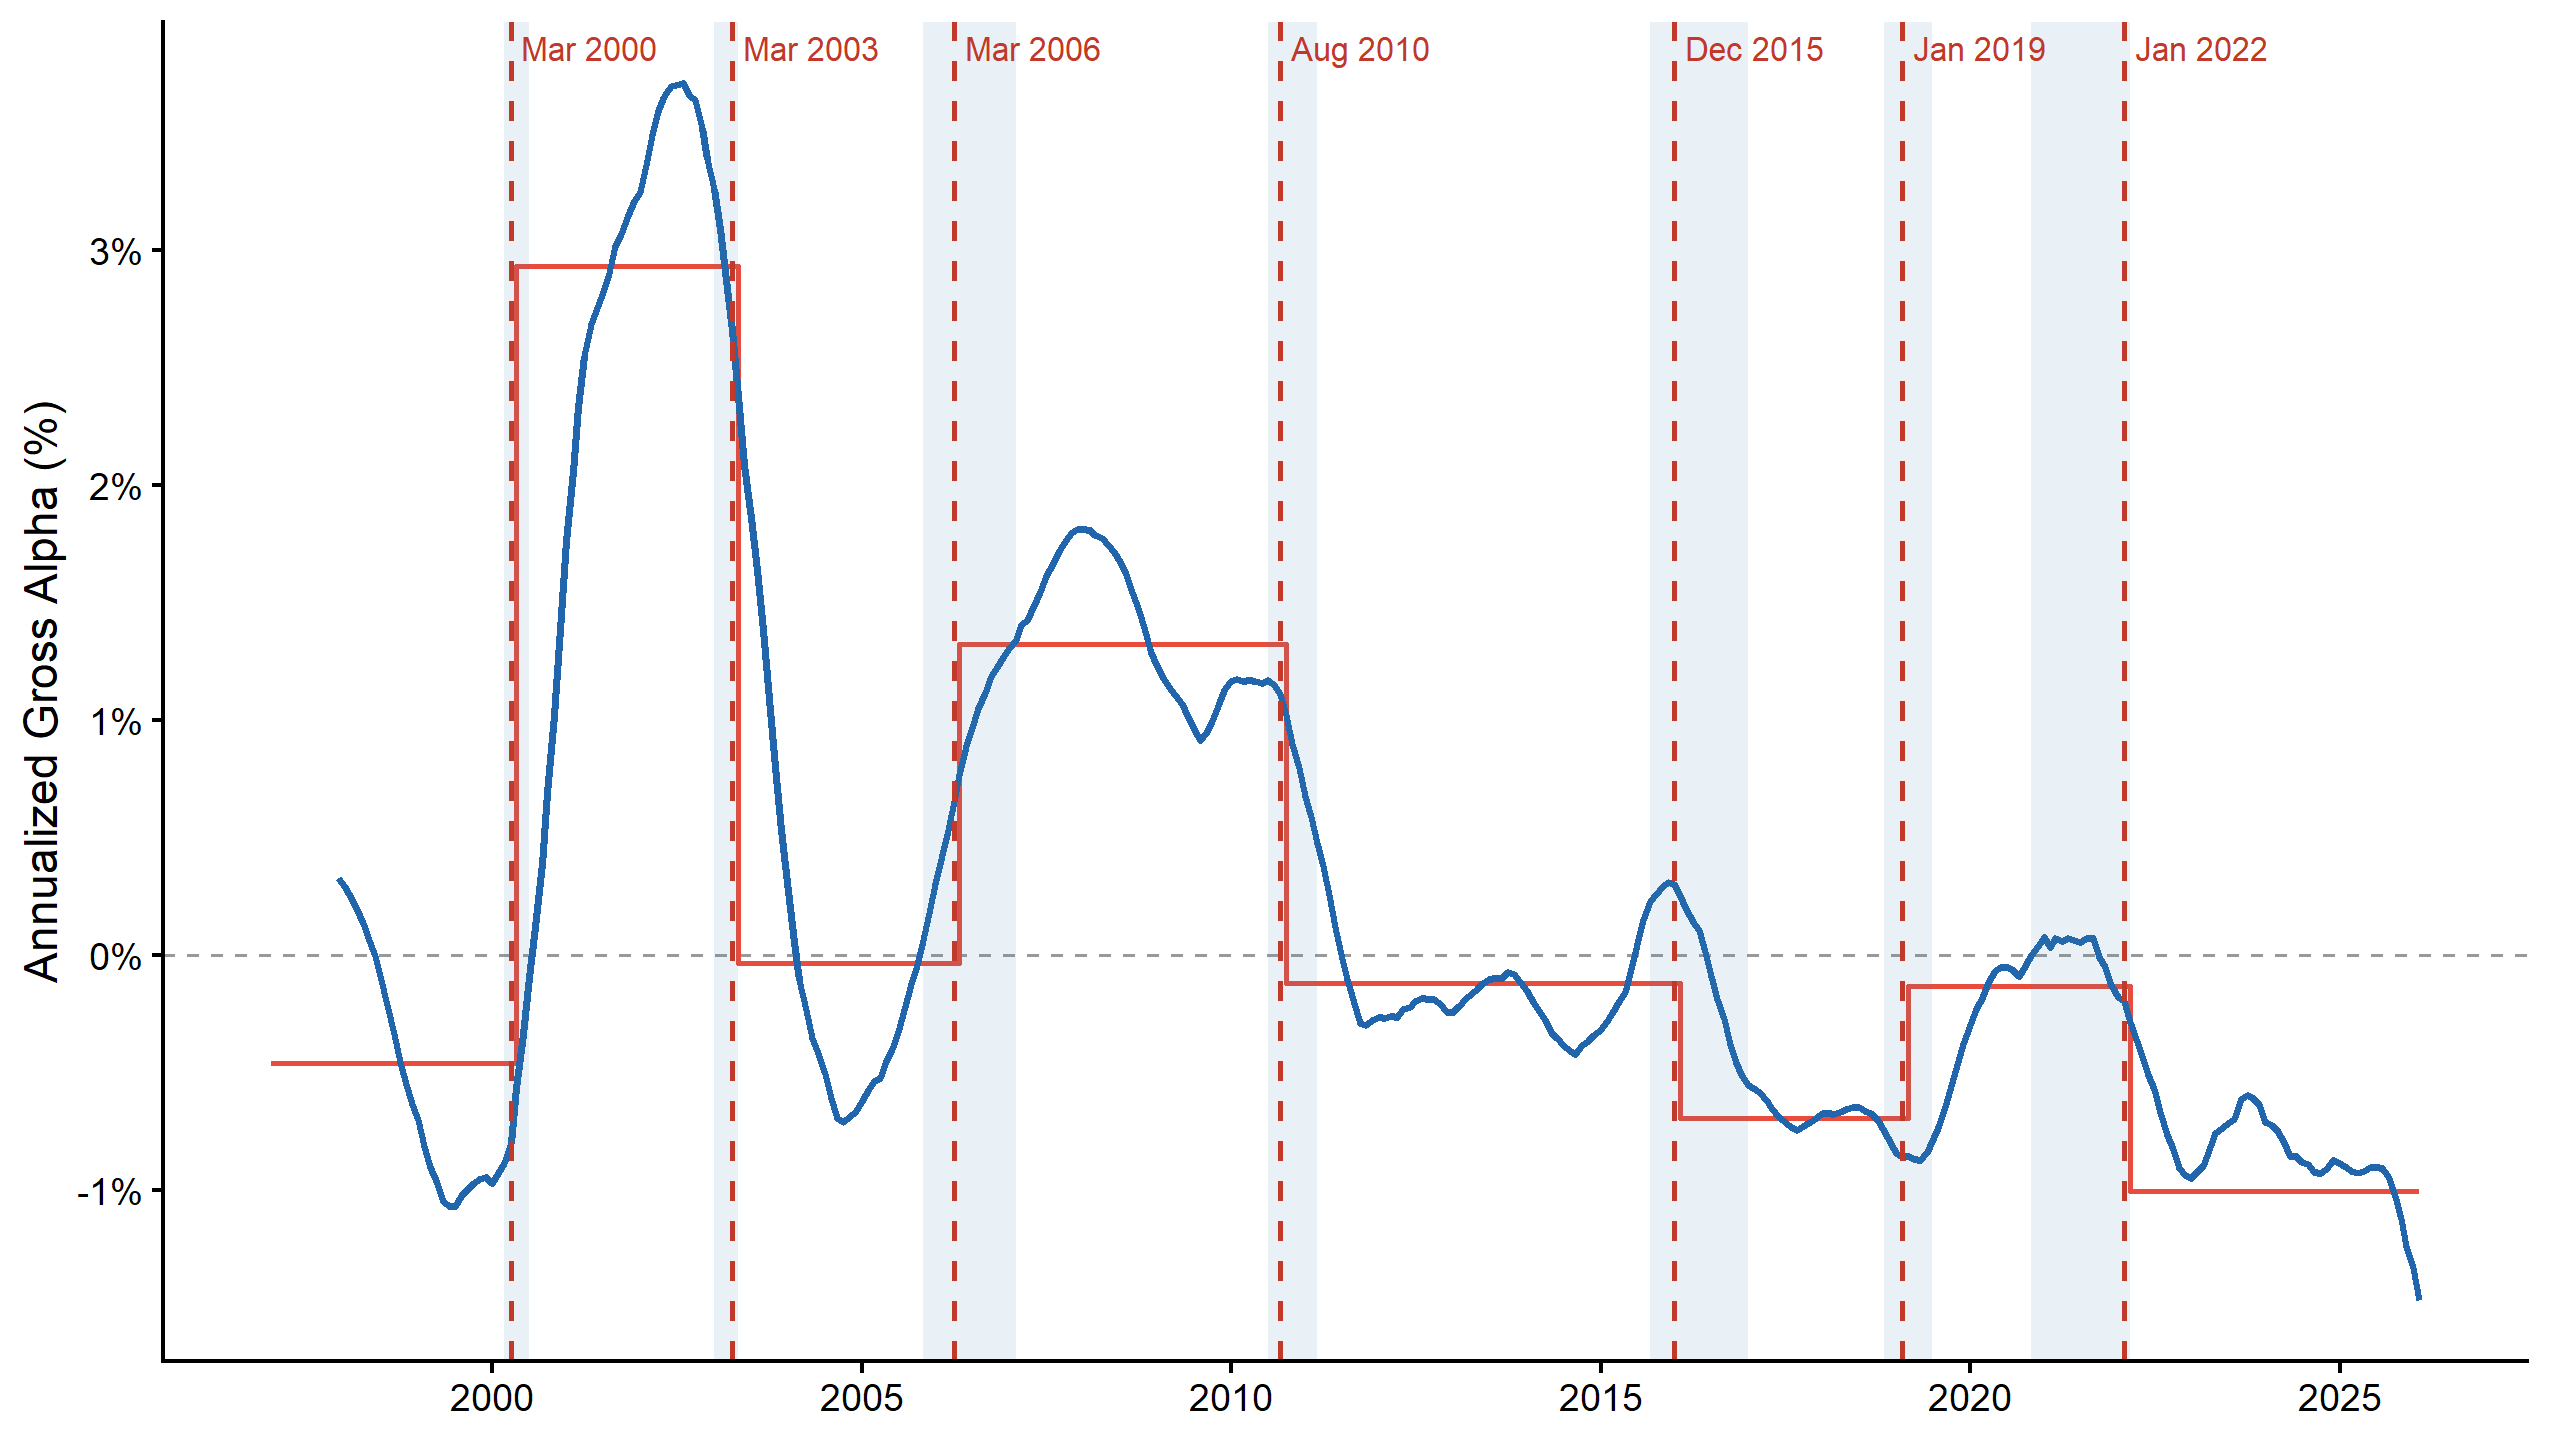
\includegraphics[width=\textwidth]{tables/fig_breaktest.png}
  \caption[Bai--Perron structural break test --- active fund rolling gross alpha]{%
    Bai--Perron structural break test on the monthly cross-sectional
    equal-weighted mean of 36-month rolling \textcite{Carhart1997}
    gross alpha for active funds. The blue line is the 12-month
    trailing mean of that cross-sectional series, plotted for
    readability; the solid red step function is the regime-mean alpha
    per identified segment; dashed red verticals are the
    \textcite{Bai1998,Bai2003} break-date point estimates; shaded bands
    are 95\,\% confidence intervals constructed using Newey--West HAC
    standard errors with a lag of 35 months, the overlap of consecutive
    36-month windows. The break test itself is applied to the raw
    (unsmoothed) monthly series. BIC selects seven breaks (March 2000,
    March 2003, March 2006, August 2010, December 2015, January 2019,
    January 2022). Each break is dated at the end of the rolling window,
    so the underlying change can precede the marked date by up to 35
    months. Sample: Incubation-corrected (Evans 2010) panel, active funds
    only, performance-comparison subsample per flagged\_funds.xlsx,
    rolling windows ending December 1996 to January 2026.}
  \label{fig:breaktest}
\end{figure}

\begin{table}[htbp]
\centering
% Phase 2.4: savebox+minipage pattern — caption left-aligns to table edge.
\sbox{\tabletempbox}{%
\footnotesize
\begin{tabular}{clccc}
\toprule
Break & Point Estimate & 95\,\% CI Lower & 95\,\% CI Upper
      & Regime Mean (\% p.a.) \\
\midrule
1 & Mar 2000 & Feb 2000  & Jun 2000  & --- \\
2 & Mar 2003 & Dec 2002  & Apr 2003  & --- \\
3 & Mar 2006 & Oct 2005  & Jan 2007  & --- \\
4 & Aug 2010 & Jun 2010  & Feb 2011  & --- \\
5 & Dec 2015 & Aug 2015  & Dec 2016  & --- \\
6 & Jan 2019 & Oct 2018  & Jun 2019  & --- \\
7 & Jan 2022 & Oct 2020  & Feb 2022  & --- \\
\midrule
\multicolumn{5}{l}{Implied eight-regime partition (rolling-window end dates):} \\[3pt]
\multicolumn{4}{l}{Regime 1: Dec 1996 -- Mar 2000 \hfill (40 months)}
    & $-0.46$ \\
\multicolumn{4}{l}{Regime 2: Apr 2000 -- Mar 2003 \hfill (36 months)}
    & $+2.93$ \\
\multicolumn{4}{l}{Regime 3: Apr 2003 -- Mar 2006 \hfill (36 months)}
    & $-0.03$ \\
\multicolumn{4}{l}{Regime 4: Apr 2006 -- Aug 2010 \hfill (53 months)}
    & $+1.33$ \\
\multicolumn{4}{l}{Regime 5: Sep 2010 -- Dec 2015 \hfill (64 months)}
    & $-0.12$ \\
\multicolumn{4}{l}{Regime 6: Jan 2016 -- Jan 2019 \hfill (37 months)}
    & $-0.69$ \\
\multicolumn{4}{l}{Regime 7: Feb 2019 -- Jan 2022 \hfill (36 months)}
    & $-0.13$ \\
\multicolumn{4}{l}{Regime 8: Feb 2022 -- Jan 2026 \hfill (48 months)}
    & $-1.00$ \\
\midrule
\multicolumn{5}{l}{Sub-periods adopted in Section~\ref{sec:subperiod_panels} (calendar months of fund returns):} \\[3pt]
\multicolumn{5}{l}{P1: Jan 1995 -- Mar 2006 (135 months); P2: Apr 2006 -- Aug 2010 (53 months);} \\
\multicolumn{5}{l}{P3: Sep 2010 -- Jan 2026 (185 months)} \\
\bottomrule
\end{tabular}%
}
\setlength{\tabletempwidth}{\wd\tabletempbox}
\ifdim\tabletempwidth>\linewidth\setlength{\tabletempwidth}{\linewidth}\fi
\begin{minipage}{\tabletempwidth}
\captionsetup{width=\linewidth}
\caption{Bai--Perron Break Dates, 95\,\% HAC Confidence Intervals, and
         Regime-Mean Gross Alpha}
\label{tab:breaktest}
\ifdim\wd\tabletempbox>\linewidth
  \resizebox{\linewidth}{!}{\usebox{\tabletempbox}}
\else
  \usebox{\tabletempbox}
\fi
\par\medskip
\begin{singlespace}\footnotesize\noindent
Note: Break dates estimated via \textcite{Bai1998} and
\textcite{Bai2003} with a minimum segment of 36 months and up to eight
breaks searched. The BIC selects seven breaks (BIC 591.1, against 601.2
for five and 601.9 for six); the criterion of \textcite{LiuWuZidek1997}
selects five. Tests of no break against one break: sup-$F = 14.82$
($p = 0.003$), mean-$F = 6.81$ ($p < 0.001$), exp-$F = 4.73$
($p < 0.001$) \parencite{Andrews1993,AndrewsPloberger1994}; the
single-break sup-$F$ is maximised in August 2021. Confidence intervals
and $F$-statistics use Newey--West HAC standard errors with a lag of 35
months, because consecutive 36-month rolling alphas share 35 months.
Regime means are equal-weighted cross-sectional means of the monthly
36-month rolling \textcite{Carhart1997} gross alpha across active funds
within each segment, annualised ($\times 12$, \%). Sample: monthly EW
mean active-fund rolling gross alpha, rolling windows ending December
1996 to January 2026 ($T = 350$ months).
\end{singlespace}
\end{minipage}
\end{table}

\noindent The BIC solution identifies seven breaks, but the criterion
is nearly flat between five and seven breaks, and the more conservative
\textcite{LiuWuZidek1997} criterion selects five; the number of breaks is
therefore not sharply determined. The regime means describe large swings
before 2010 --- a negative late-1990s segment, a strongly positive segment
whose rolling windows contain the technology-stock collapse
(+2.93\% per annum), a segment near zero, and a positive segment ending in
August 2010 (+1.33\%) --- and four segments after 2010 that are all at or
below zero. The August 2010 break, with a confidence interval of June
2010--February 2011, marks the transition between the last positive
segment and the post-2010 period, with a fall in the regime mean of about
1.4 percentage points.

Two features of the break evidence limit its interpretation. First,
because the rolling alphas overlap, the input series is smooth by
construction, and break tests on smooth series tend to find many breaks.
The confidence intervals above use a HAC lag equal to the overlap; an
earlier version of this analysis, on the previous data construction,
used a data-driven lag of five months and produced narrower intervals and an $F$-statistic several times
larger (sup-$F$ of 53.4). Second, each break is dated at the end of a 36-month
window, so the underlying change may have occurred up to 35 months
earlier; the deterioration marked in August 2010 may therefore have begun
as early as late 2007.

As a robustness check, the test is applied to the non-overlapping monthly
abnormal return of the equal-weighted active portfolio --- its gross
excess return minus the fitted full-sample Carhart factor component ---
over January 1995--January 2026 ($T = 373$, HAC lag 12). On this series
the BIC selects no break. The single-break sup-$F$ statistic is 10.67
($p = 0.019$) and is maximised in August 2019, so the null of complete
stability is rejected, but the evidence for a mean shift is weaker and
its date is later than in the rolling series. The monthly abnormal return
is noisy, and a shift of one or two percentage points per annum in its
mean is difficult to date precisely; the two results are therefore
consistent with a gradual deterioration in the 2010s rather than a
single sharp break.

The sub-periods are defined accordingly. Two of the rolling-series
breaks are used as boundaries: March 2006, which separates the volatile
pre-2006 segments from the positive 2006--2010 segment, and August 2010,
which separates that segment from the post-2010 period. The 2000 and
2003 breaks define segments of only 36 months and are pooled into P1;
the 2015, 2019 and 2022 breaks are pooled into P3 because every post-2010
segment has a regime mean at or below zero. The resulting sub-periods,
expressed in calendar months of fund returns, are P1 (January
1995--March 2006, 135 months), P2 (April 2006--August 2010, 53 months),
and P3 (September 2010--January 2026, 185 months). P2 is shorter than the
60 months that \textcite{BarrasScailletWermers2010} recommend for
fund-level inference, and its results should be read with corresponding
caution.

\section{Sub-period performance and skill decomposition}
\label{sec:subperiod_panels}

\noindent This section reports the full set of sub-period performance
tables, estimated separately within P1 (January 1995--March 2006), P2
(April 2006--August 2010), and P3 (September 2010--January 2026). The
bootstrap and false-discovery results use the funds with at least 24
monthly observations within each sub-period.

\begin{table}[!htbp]
\centering
\sbox{\tabletempbox}{%
\footnotesize
\setlength{\tabcolsep}{4pt}%
\begin{tabular}[t]{lrrrrrr}
\toprule
\multicolumn{3}{c}{ } & \multicolumn{2}{c}{Gross Alpha} & \multicolumn{2}{c}{Net Alpha} \\
\cmidrule(l{3pt}r{3pt}){4-5} \cmidrule(l{3pt}r{3pt}){6-7}
Group & $N$ & $T$ & EW & VW & EW & VW\\
\midrule
\addlinespace[0.3em]
\multicolumn{7}{l}{\textit{Panel A: P1 (Jan 1995--Mar 2006, 135 months)}}\\
\hspace{1em}Active & 884 & 135 & 0.284 & 0.016 & -0.741 & -0.611\\
\hspace{1em}t(coef) &  &  & (0.34) & (0.02) & (-0.88) & (-0.90)\\
\hspace{1em}Passive & 128 & 135 & 0.220 & 0.499 & -0.180 & 0.382\\
\hspace{1em}t(coef) &  &  & (0.44) & (1.61) & (-0.36) & (1.22)\\
\hspace{1em}Unknown & 492 & 135 & -1.306$^{*}$ & -4.199$^{***}$ & -2.659$^{***}$ & -5.384$^{***}$\\
\hspace{1em}t(coef) &  &  & (-1.65) & (-2.72) & (-3.36) & (-3.40)\\
\midrule
\hspace{1em}Active + Passive & 1,012 & 135 & 0.260 & 0.086 & -0.705 & -0.439\\
\hspace{1em}t(coef) &  &  & (0.33) & (0.15) & (-0.89) & (-0.78)\\
\hspace{1em}Full Sample & 1,504 & 135 & -0.126 & 0.085 & -1.173 & -0.444\\
\hspace{1em}t(coef) &  &  & (-0.16) & (0.15) & (-1.51) & (-0.79)\\
\addlinespace[0.3em]
\hline
\multicolumn{7}{l}{\textit{Panel B: P2 (Apr 2006--Aug 2010, 53 months)}}\\
\hspace{1em}Active & 1,129 & 53 & 0.894 & 0.067 & -0.169 & -0.688\\
\hspace{1em}t(coef) &  &  & (1.24) & (0.08) & (-0.23) & (-0.87)\\
\hspace{1em}Passive & 137 & 53 & 0.169 & 0.235 & -0.304 & 0.097\\
\hspace{1em}t(coef) &  &  & (0.42) & (0.92) & (-0.77) & (0.38)\\
\hspace{1em}Unknown & 396 & 53 & -1.904$^{***}$ & -0.600 & -3.247$^{***}$ & -1.686$^{***}$\\
\hspace{1em}t(coef) &  &  & (-2.92) & (-0.97) & (-5.01) & (-2.76)\\
\midrule
\hspace{1em}Active + Passive & 1,266 & 53 & 0.814 & 0.134 & -0.187 & -0.531\\
\hspace{1em}t(coef) &  &  & (1.20) & (0.19) & (-0.28) & (-0.77)\\
\hspace{1em}Full Sample & 1,662 & 53 & 0.412 & 0.121 & -0.643 & -0.550\\
\hspace{1em}t(coef) &  &  & (0.63) & (0.18) & (-0.99) & (-0.81)\\
\addlinespace[0.3em]
\hline
\multicolumn{7}{l}{\textit{Panel C: P3 (Sep 2010--Jan 2026, 185 months)}}\\
\hspace{1em}Active & 1,950 & 185 & -0.698$^{*}$ & -0.292 & -1.754$^{***}$ & -0.995$^{***}$\\
\hspace{1em}t(coef) &  &  & (-1.72) & (-0.94) & (-4.32) & (-3.20)\\
\hspace{1em}Passive & 237 & 185 & -0.583$^{**}$ & -0.196 & -1.022$^{***}$ & -0.284$^{*}$\\
\hspace{1em}t(coef) &  &  & (-2.10) & (-1.18) & (-3.69) & (-1.70)\\
\hspace{1em}Unknown & 169 & 185 & -2.028$^{*}$ & -3.387$^{**}$ & -3.294$^{***}$ & -4.461$^{***}$\\
\hspace{1em}t(coef) &  &  & (-1.71) & (-2.00) & (-2.79) & (-2.64)\\
\midrule
\hspace{1em}Active + Passive & 2,187 & 185 & -0.687$^{*}$ & -0.275 & -1.678$^{***}$ & -0.827$^{***}$\\
\hspace{1em}t(coef) &  &  & (-1.78) & (-1.11) & (-4.35) & (-3.34)\\
\hspace{1em}Full Sample & 2,356 & 185 & -0.738$^{*}$ & -0.276 & -1.734$^{***}$ & -0.829$^{***}$\\
\hspace{1em}t(coef) &  &  & (-1.93) & (-1.12) & (-4.54) & (-3.35)\\
\bottomrule
\end{tabular}%
}
\setlength{\tabletempwidth}{\wd\tabletempbox}
\ifdim\tabletempwidth>\linewidth\setlength{\tabletempwidth}{\linewidth}\fi
\begin{minipage}{\tabletempwidth}
\captionsetup{width=\linewidth}
\caption{\label{tab:subperiod_perf_aggregate}Aggregate Portfolio Alpha by Group and Sub-Period (\%, Annualised)}
\ifdim\wd\tabletempbox>\linewidth
  \resizebox{\linewidth}{!}{\usebox{\tabletempbox}}
\else
  \usebox{\tabletempbox}
\fi
\par\medskip
\begin{singlespace}\footnotesize\noindent
Annualised \textcite{Carhart1997} four-factor alpha (\%) from portfolio regressions of the monthly aggregate return of each group on the market, size, value, and momentum factors, estimated separately within each sub-period, following \textcite{FamaFrench2010}. EW: equal-weighted; VW: lagged-TNA-weighted $w_{i,t-1} = \text{TNA}_{i,t-1} / \sum_j \text{TNA}_{j,t-1}$. Net = gross $-$ expense/12 \parencite{Carhart1997, Wermers2000}. Newey-West $t$-stats (6-month lag) in parentheses; $^{*}$, $^{**}$, $^{***}$: 10\%, 5\%, 1\%. $N$: unique funds; $T$: months in the regression. Sub-period thresholds (Jan 2006, Oct 2011) from Bai-Perron test (Section D.1). Sample: Incubation-corrected panel (Evans 2010), no date cap; performance-comparison subsample per flagged\_funds.xlsx.
\end{singlespace}
\end{minipage}
\end{table}



\begin{table}[!htbp]
\centering
\sbox{\tabletempbox}{%
\footnotesize
\setlength{\tabcolsep}{4pt}%
\begin{tabular}[t]{rrrr>{\raggedright\arraybackslash}p{13em}}
\toprule
Percentile & Actual $t(\hat{\alpha})$ & Sim.\ Mean & Prob.\ Luck & Interpretation\\
\midrule
\multicolumn{5}{l}{\textit{Panel A: P1 (Jan 1995--Mar 2006, 135 months)}}\\
\hspace{1em}1\% & -2.400 & -2.911 & 84.6\% & Consistent with zero skill\\
\hspace{1em}5\% & -1.709 & -1.895 & 67.2\% & Consistent with zero skill\\
\hspace{1em}10\% & -1.227 & -1.435 & 71.6\% & Consistent with zero skill\\
\hspace{1em}50\% & 0.123 & 0.023 & 63.4\% & Consistent with zero skill\\
\hspace{1em}90\% & 1.671 & 1.486 & 72.5\% & Consistent with zero skill\\
\hspace{1em}95\% & 2.211 & 1.953 & 76.1\% & Consistent with zero skill\\
\hspace{1em}99\% & 3.271 & 3.011 & 70.3\% & Consistent with zero skill\\
\hline
\multicolumn{5}{l}{\textit{Panel B: P2 (Apr 2006--Aug 2010, 53 months)}}\\
\hspace{1em}1\% & -3.015 & -2.914 & 39.1\% & Consistent with zero skill\\
\hspace{1em}5\% & -1.894 & -1.947 & 50.0\% & Consistent with zero skill\\
\hspace{1em}10\% & -1.268 & -1.484 & 67.6\% & Consistent with zero skill\\
\hspace{1em}50\% & 0.415 & 0.009 & 88.0\% & Consistent with zero skill\\
\hspace{1em}90\% & 1.912 & 1.511 & 83.5\% & Consistent with zero skill\\
\hspace{1em}95\% & 2.359 & 1.980 & 80.4\% & Consistent with zero skill\\
\hspace{1em}99\% & 3.407 & 2.973 & 77.4\% & Consistent with zero skill\\
\hline
\multicolumn{5}{l}{\textit{Panel C: P3 (Sep 2010--Jan 2026, 185 months)}}\\
\hspace{1em}1\% & -3.427 & -2.645 & 3.8\% & Worse than luck\\
\hspace{1em}5\% & -2.393 & -1.744 & 5.0\% & Consistent with zero skill\\
\hspace{1em}10\% & -1.980 & -1.335 & 4.6\% & Worse than luck\\
\hspace{1em}50\% & -0.536 & 0.017 & 5.3\% & Consistent with zero skill\\
\hspace{1em}90\% & 0.931 & 1.380 & 8.8\% & Consistent with zero skill\\
\hspace{1em}95\% & 1.366 & 1.794 & 11.1\% & Consistent with zero skill\\
\hspace{1em}99\% & 2.175 & 2.689 & 8.9\% & Consistent with zero skill\\
\bottomrule
\end{tabular}%
}
\setlength{\tabletempwidth}{\wd\tabletempbox}
\ifdim\tabletempwidth>\linewidth\setlength{\tabletempwidth}{\linewidth}\fi
\begin{minipage}{\tabletempwidth}
\captionsetup{width=\linewidth}
\caption{\label{tab:subperiod_bootstrap_tails}Fama--French (2010) Bootstrap: Actual vs.\ Simulated $t(\hat{\alpha})$ Percentiles by Sub-Period}
\ifdim\wd\tabletempbox>\linewidth
  \resizebox{\linewidth}{!}{\usebox{\tabletempbox}}
\else
  \usebox{\tabletempbox}
\fi
\par\medskip
\begin{singlespace}\footnotesize\noindent
Bootstrap procedure follows \textcite{FamaFrench2010}, applied separately within each sub-period. For each fund, estimated monthly alpha is subtracted from the excess return series to construct a zero-alpha null return. In each of $B = 10{,}000$ bootstrap iterations, calendar months (within the sub-period window) are resampled with replacement and kept in the order drawn, the same draw applying to all funds, preserving cross-sectional factor return dependence. The \textcite{Carhart1997} four-factor model is re-estimated on each resampled series. \textit{Actual} $t(\hat{\alpha})$: percentile of the empirical $t$-statistic distribution across active funds in the sub-period. \textit{Sim.\ Mean}: average of that percentile across all iterations. \textit{Prob.\ Luck}: fraction of iterations in which the simulated percentile falls below the actual value; values below 5\% (above 95\%) indicate that the actual percentile is worse (better) than zero-alpha luck would produce; 0.0\% means no iteration and $<$0.1\% means 1 to 4 of 10,000. Newey-West standard errors with a 6-month lag are used throughout. Active fund counts: P1 $N = 772$; P2 $N = 1,018$; P3 $N = 1,799$. Sample: Incubation-corrected panel (Evans 2010), no date cap; performance-comparison subsample per flagged\_funds.xlsx.
\end{singlespace}
\end{minipage}
\end{table}



\begin{table}[!htbp]
\centering
\sbox{\tabletempbox}{%
\footnotesize
\setlength{\tabcolsep}{4pt}%
\begin{tabular}[t]{>{\raggedright\arraybackslash}p{13em}rrr>{\raggedright\arraybackslash}p{14em}}
\toprule
Sub-Period & $\hat{\pi}_0$ & $N$ & $\lambda$ & Interpretation\\
\midrule
P1 (Jan 1995--Mar 2006) & 86.0\% & 772 & 0.5 & Heterogeneous skill; majority zero-alpha\\
P2 (Apr 2006--Aug 2010) & 80.9\% & 1,018 & 0.5 & Heterogeneous skill; majority zero-alpha\\
P3 (Sep 2010--Jan 2026) & 81.0\% & 1,799 & 0.5 & Heterogeneous skill; majority zero-alpha\\
\bottomrule
\end{tabular}%
}
\setlength{\tabletempwidth}{\wd\tabletempbox}
\ifdim\tabletempwidth>\linewidth\setlength{\tabletempwidth}{\linewidth}\fi
\begin{minipage}{\tabletempwidth}
\captionsetup{width=\linewidth}
\caption{\label{tab:subperiod_pi0_estimate}Aggregate Skill Estimate by Sub-Period: Proportion of True Zero-Alpha Active Funds}
\ifdim\wd\tabletempbox>\linewidth
  \resizebox{\linewidth}{!}{\usebox{\tabletempbox}}
\else
  \usebox{\tabletempbox}
\fi
\par\medskip
\begin{singlespace}\footnotesize\noindent
The proportion of true zero-alpha active funds ($\hat{\pi}_0$) estimated separately within each sub-period, following \textcite{Storey2002} and \textcite{BarrasScailletWermers2010}, using $p$-values from Newey-West $t$-tests on sub-period \textcite{Carhart1997} four-factor alphas. The estimator is $\hat{\pi}_0 = |\{p_i > \lambda\}| \,/\, [N(1-\lambda)]$, where $\lambda = 0.5$ is the standard tuning parameter. $N$: number of active funds with $\geq 24$ monthly observations within the sub-period. Passive and Unknown-classified funds are excluded. Sample: Incubation-corrected panel (Evans 2010), no date cap; performance-comparison subsample per flagged\_funds.xlsx. The four-way decomposition of skilled, unskilled, and lucky fund proportions implied by these estimates is reported in Table~\ref{tab:subperiod_bsw_decomposition}.
\end{singlespace}
\end{minipage}
\end{table}



\begin{table}[!htbp]
\centering
\sbox{\tabletempbox}{%
\footnotesize
\setlength{\tabcolsep}{4pt}%
\begin{tabular}[t]{rrrrrr}
\toprule
\multicolumn{1}{c}{ } & \multicolumn{2}{c}{Observed Tails} & \multicolumn{1}{c}{False Disc.} & \multicolumn{2}{c}{True Proportions} \\
\cmidrule(l{3pt}r{3pt}){2-3} \cmidrule(l{3pt}r{3pt}){4-4} \cmidrule(l{3pt}r{3pt}){5-6}
$\gamma$ & $S^-_\gamma$ & $S^+_\gamma$ & $F_\gamma$ & $T^-_\gamma$ & $T^+_\gamma$\\
\midrule
\multicolumn{6}{l}{\textit{Panel A: P1 (Jan 1995--Mar 2006, 135 months)}}\\
\hspace{1em}5\% & 3.6 & 7.3 & 2.2 & 1.5 & 5.1\\
\hspace{1em}10\% & 5.6 & 10.0 & 4.3 & 1.3 & 5.7\\
\hspace{1em}15\% & 7.9 & 14.1 & 6.5 & 1.5 & 7.7\\
\hspace{1em}20\% & 9.1 & 17.5 & 8.6 & 0.5 & 8.9\\
\hspace{1em}25\% & 11.4 & 20.3 & 10.8 & 0.6 & 9.6\\
\hspace{1em}30\% & 13.3 & 22.7 & 12.9 & 0.4 & 9.8\\
\hspace{1em}35\% & 15.9 & 25.4 & 15.1 & 0.9 & 10.3\\
\hspace{1em}40\% & 18.0 & 27.5 & 17.2 & 0.8 & 10.3\\
\hspace{1em}45\% & 20.5 & 31.9 & 19.4 & 1.1 & 12.5\\
\hspace{1em}50\% & 22.4 & 34.6 & 21.5 & 0.9 & 13.1\\
\hline
\multicolumn{6}{l}{\textit{Panel B: P2 (Apr 2006--Aug 2010, 53 months)}}\\
\hspace{1em}5\% & 4.1 & 8.8 & 2.0 & 2.1 & 6.8\\
\hspace{1em}10\% & 6.7 & 13.1 & 4.0 & 2.6 & 9.0\\
\hspace{1em}15\% & 8.7 & 18.6 & 6.1 & 2.7 & 12.5\\
\hspace{1em}20\% & 9.8 & 22.2 & 8.1 & 1.7 & 14.1\\
\hspace{1em}25\% & 11.5 & 25.8 & 10.1 & 1.4 & 15.7\\
\hspace{1em}30\% & 12.8 & 28.0 & 12.1 & 0.6 & 15.9\\
\hspace{1em}35\% & 14.6 & 30.9 & 14.2 & 0.5 & 16.8\\
\hspace{1em}40\% & 16.1 & 34.2 & 16.2 & -0.1 & 18.0\\
\hspace{1em}45\% & 17.9 & 37.6 & 18.2 & -0.3 & 19.4\\
\hspace{1em}50\% & 19.5 & 40.0 & 20.2 & -0.7 & 19.7\\
\hline
\multicolumn{6}{l}{\textit{Panel C: P3 (Sep 2010--Jan 2026, 185 months)}}\\
\hspace{1em}5\% & 9.7 & 1.4 & 2.0 & 7.6 & -0.6\\
\hspace{1em}10\% & 15.9 & 3.0 & 4.1 & 11.8 & -1.1\\
\hspace{1em}15\% & 21.2 & 4.6 & 6.1 & 15.2 & -1.5\\
\hspace{1em}20\% & 25.0 & 5.9 & 8.1 & 16.9 & -2.2\\
\hspace{1em}25\% & 29.2 & 7.3 & 10.1 & 19.1 & -2.8\\
\hspace{1em}30\% & 32.5 & 8.5 & 12.2 & 20.3 & -3.7\\
\hspace{1em}35\% & 35.9 & 9.9 & 14.2 & 21.7 & -4.3\\
\hspace{1em}40\% & 39.6 & 11.3 & 16.2 & 23.4 & -4.9\\
\hspace{1em}45\% & 41.9 & 12.6 & 18.2 & 23.6 & -5.6\\
\hspace{1em}50\% & 45.1 & 14.4 & 20.3 & 24.8 & -5.9\\
\bottomrule
\end{tabular}%
}
\setlength{\tabletempwidth}{\wd\tabletempbox}
\ifdim\tabletempwidth>\linewidth\setlength{\tabletempwidth}{\linewidth}\fi
\begin{minipage}{\tabletempwidth}
\captionsetup{width=\linewidth}
\caption{\label{tab:subperiod_bsw_decomposition}BSW (2010) Four-Way Decomposition by Sub-Period: Proportions of Skilled, Unskilled, and Lucky Funds (\%)}
\ifdim\wd\tabletempbox>\linewidth
  \resizebox{\linewidth}{!}{\usebox{\tabletempbox}}
\else
  \usebox{\tabletempbox}
\fi
\par\medskip
\begin{singlespace}\footnotesize\noindent
\textcite{BarrasScailletWermers2010} four-way decomposition, estimated separately within each sub-period. $S^-_\gamma$ ($S^+_\gamma$): fraction of active funds with significantly negative (positive) Newey-West $t(\hat{\alpha})$ at two-sided level $\gamma$, using sub-period \textcite{Carhart1997} alphas and the same Student-$t$ $p$-values as $\hat{\pi}_0$. $F_\gamma = \hat{\pi}_0 \cdot \gamma/2$: expected false discoveries per tail, with $\hat{\pi}_0$ the sub-period \textcite{Storey2002} estimator at $\lambda = 0.5$ (Table~\ref{tab:subperiod_pi0_estimate}). $T^\pm_\gamma = S^\pm_\gamma - F_\gamma$: genuinely unskilled ($-$) or skilled ($+$). The row at $\gamma^* = 0.45$ gives population-level $\hat{\pi}^-_A$, $\hat{\pi}^+_A$ (BSW 2010, eq.~8). Negative $T^+_\gamma$ means right-tail significance does not exceed the false-discovery rate. Percentages of the sub-period active-fund universe. Sample: Incubation-corrected panel (Evans 2010), no date cap; performance-comparison subsample per flagged\_funds.xlsx.
\end{singlespace}
\end{minipage}
\end{table}



\begin{table}[!htbp]
\centering
\sbox{\tabletempbox}{%
\footnotesize
\setlength{\tabcolsep}{4pt}%
\begin{tabular}[t]{lrrr}
\toprule
Portfolio & $\alpha_{\text{CAPM}}$ & $\alpha_{\text{FF3}}$ & $\alpha_{\text{Car}}$\\
\midrule
\addlinespace[0.3em]
\multicolumn{4}{l}{\textit{Panel A: P1 (Jan 1995--Mar 2006, 135 months)}}\\
\hspace{1em}Active (EW) & 2.542$^{*}$ & 0.180 & 0.284\\
\hspace{1em}t(coef) & (1.73) & (0.27) & (0.34)\\
\hspace{1em}Active (VW) & 0.977 & 0.209 & 0.016\\
\hspace{1em}t(coef) & (1.47) & (0.32) & (0.02)\\
\hspace{1em}Passive (EW) & 1.183 & -0.208 & 0.220\\
\hspace{1em}t(coef) & (1.56) & (-0.48) & (0.44)\\
\hspace{1em}Passive (VW) & 0.410 & 0.131 & 0.499\\
\hspace{1em}t(coef) & (0.75) & (0.44) & (1.61)\\
\addlinespace[0.3em]
\hline
\multicolumn{4}{l}{\textit{Panel B: P2 (Apr 2006--Aug 2010, 53 months)}}\\
\hspace{1em}Active (EW) & 1.305 & 1.066 & 0.894\\
\hspace{1em}t(coef) & (1.27) & (1.58) & (1.24)\\
\hspace{1em}Active (VW) & 0.437 & 0.281 & 0.067\\
\hspace{1em}t(coef) & (0.46) & (0.34) & (0.08)\\
\hspace{1em}Passive (EW) & 0.408 & 0.333 & 0.169\\
\hspace{1em}t(coef) & (0.49) & (1.10) & (0.42)\\
\hspace{1em}Passive (VW) & 0.482 & 0.496 & 0.235\\
\hspace{1em}t(coef) & (1.12) & (1.27) & (0.92)\\
\addlinespace[0.3em]
\hline
\multicolumn{4}{l}{\textit{Panel C: P3 (Sep 2010--Jan 2026, 185 months)}}\\
\hspace{1em}Active (EW) & -1.716$^{**}$ & -0.644 & -0.698$^{*}$\\
\hspace{1em}t(coef) & (-2.01) & (-1.54) & (-1.72)\\
\hspace{1em}Active (VW) & -0.503 & -0.249 & -0.292\\
\hspace{1em}t(coef) & (-1.37) & (-0.79) & (-0.94)\\
\hspace{1em}Passive (EW) & -1.320$^{**}$ & -0.532$^{*}$ & -0.583$^{**}$\\
\hspace{1em}t(coef) & (-2.02) & (-1.88) & (-2.10)\\
\hspace{1em}Passive (VW) & -0.102 & -0.165 & -0.196\\
\hspace{1em}t(coef) & (-0.41) & (-0.95) & (-1.18)\\
\bottomrule
\end{tabular}%
}
\setlength{\tabletempwidth}{\wd\tabletempbox}
\ifdim\tabletempwidth>\linewidth\setlength{\tabletempwidth}{\linewidth}\fi
\begin{minipage}{\tabletempwidth}
\captionsetup{width=\linewidth}
\caption{\label{tab:subperiod_port_agg_alpha}Active vs.\ Passive Aggregate Portfolio Alpha by Sub-Period (\%, Annualised)}
\ifdim\wd\tabletempbox>\linewidth
  \resizebox{\linewidth}{!}{\usebox{\tabletempbox}}
\else
  \usebox{\tabletempbox}
\fi
\par\medskip
\begin{singlespace}\footnotesize\noindent
Monthly EW and VW aggregate portfolio returns regressed on CAPM, Fama-French three-factor, and \textcite{Carhart1997} four-factor models, estimated separately within each sub-period. Alphas annualised ($\times 12$) and expressed as \%. Newey-West $t$-statistics (6-month lag) in parentheses. $^{*}$, $^{**}$, $^{***}$: significant at 10\%, 5\%, 1\% respectively. Sample: Incubation-corrected panel (Evans 2010), no date cap; performance-comparison subsample per flagged\_funds.xlsx.
\end{singlespace}
\end{minipage}
\end{table}



\noindent The sub-periods differ sharply. In P1 and P2 the aggregate
active portfolio earns positive but insignificant gross alphas
($+0.28\%$ and $+0.89\%$ per annum EW) and insignificant net alphas
($-0.74\%$ and $-0.17\%$), and no bootstrap percentile is distinguishable
from zero skill. The false-discovery decomposition nevertheless finds a
detectable skilled minority: at $\gamma^* = 0.45$, $\hat{\pi}^+_A$ is
12.5\% in P1 and 19.4\% in P2, while $\hat{\pi}^-_A$ is 1.1\% and
$-0.3\%$. The skilled share is positive at every threshold in both
sub-periods.

In P3 the picture reverses. The aggregate active portfolio earns an EW
gross alpha of $-0.70\%$ per annum (significant at 10\%), and EW and VW
net alphas of $-1.75\%$ and $-1.00\%$ (both significant at 1\%). The
left tail of the bootstrap distribution is worse than luck at the 1st and
10th percentiles (Prob.\ Luck 3.8\% and 4.6\%) and at the margin at the
5th (5.0\%), and the actual right-tail percentiles are below their
simulated counterparts throughout. The unskilled share is 23.6\% and the
skilled share is negative ($-5.6\%$) at $\gamma^* = 0.45$, so that
right-tail significance falls short of the false-discovery rate. The
$\hat{\pi}_0$ estimates are similar across sub-periods (86.0\%, 80.9\%
and 81.0\%); what changes is the sign of the non-zero-alpha mass.
Passive funds also underperform in P3 (EW net $-1.02\%$), but the active
shortfall exceeds the passive one by about 0.7 percentage points on both
weightings.

% --- Appendix I --------------------------------------------------------------
\chapter{FACTOR MODEL ROBUSTNESS}
\label{app:robustness}

\noindent This appendix re-estimates the core performance results
under two alternative factor-model specifications: the
\textcite{FamaFrench2015} five-factor model augmented with momentum
(FF6: $\text{MKT} - \text{Rf}$, $\text{SMB}$, $\text{HML}$,
$\text{RMW}$, $\text{CMA}$, $\text{MOM}$) and the Carhart
four-factor model augmented with the
\textcite{PastorStambaugh2003} traded liquidity factor (Carhart$+$PSL:
$\text{MKT} - \text{Rf}$, $\text{SMB}$, $\text{HML}$,
$\text{MOM}$, $\text{LIQ}_V$). The robustness exercise is
confined to the full-period pooled alpha, bootstrap, and BSW
decomposition components; the rolling-alpha series, flow--performance
regressions, and sub-period analyses are not re-estimated under
alternative factor models. The defensive scope reflects the focus of
the robustness exercise: whether the puzzle survives factor-model
choice, not whether every downstream result is factor-invariant.

The motivation for the robustness exercise is the legitimate question
raised by the committee during preparation meetings: whether the
main-text Carhart four-factor alpha estimates are robust to factor
model choice, specifically referencing the
\textcite{FamaFrench2015} five-factor model and the
\textcite{PastorStambaugh2003} traded liquidity factor. A
defensive response is warranted: if pooled active-fund alpha proves
materially different under FF6 or Carhart$+$PSL, the main empirical
argument of the dissertation would require qualification.

The Fama--French SMB construction is held constant across all three
specifications (FF3/Carhart construction, single $2 \times 3$ size-BM
sort). The FF5 release provides a different SMB (averaged across
three $2 \times 3$ sorts), but the two series correlate above 0.97
over December 1994 through December 2024. Holding SMB constant
isolates the marginal effect of adding RMW and CMA without conflating
it with an SMB definition change. Per-specification sample filtering
is applied: each specification's regression uses the maximum
available sample for its own factor set; a shared filter would
unnecessarily truncate FF6 to the PSL coverage window (through
December 2024 only). The Carhart$+$PSL specification is therefore
estimated on a slightly shorter sample than the Carhart and FF6
specifications. Symmetric Newey--West standard errors at six-month
lag are applied uniformly to actual and bootstrap-simulated
$t$-statistics, matching the main-text procedure. Defensive $-99$
sentinel handling is applied to the raw Pástor file: pre-1968 missing
values (coded as $-99$) are converted to NA at panel preparation; the
period is outside the sample window so there is no effective impact,
but the guard is in place.

\begin{table}[!htbp]
\centering
\sbox{\tabletempbox}{%
\footnotesize
\begin{tabular}{llrrrrrrr}
\toprule
 & & & & \multicolumn{2}{c}{Gross Alpha} & \multicolumn{2}{c}{Net Alpha} & \\
\cmidrule(lr){5-6} \cmidrule(lr){7-8}
Model & Group & $N$ & $T$ & EW & VW & EW & VW & $\bar{R}^2$ \\
\midrule
Carhart 4-Factor & Active & 1,952 & 373 & 0.223 & 0.027 & -0.823$^{*}$ & -0.658 & 0.982 \\
t(coef) &  &  &  & (0.47) & (0.07) & (-1.75) & (-1.62) &  \\
 & Passive & 269 & 373 & -0.262 & 0.049 & -0.693$^{**}$ & -0.057 & 0.991 \\
t(coef) &  &  &  & (-0.96) & (0.29) & (-2.54) & (-0.34) &  \\
\addlinespace
FF 6-Factor & Active & 1,952 & 373 & -0.038 & -0.101 & -1.084$^{**}$ & -0.786$^{*}$ & 0.982 \\
t(coef) &  &  &  & (-0.09) & (-0.25) & (-2.43) & (-1.94) &  \\
 & Passive & 269 & 373 & -0.599$^{**}$ & -0.266$^{*}$ & -1.029$^{***}$ & -0.372$^{**}$ & 0.992 \\
t(coef) &  &  &  & (-2.43) & (-1.69) & (-4.19) & (-2.37) &  \\
\addlinespace
Carhart + PSL & Active & 1,907 & 360 & 0.202 & -0.054 & -0.845$^{*}$ & -0.742$^{*}$ & 0.983 \\
t(coef) &  &  &  & (0.43) & (-0.13) & (-1.78) & (-1.78) &  \\
 & Passive & 265 & 360 & -0.259 & 0.074 & -0.691$^{**}$ & -0.035 & 0.991 \\
t(coef) &  &  &  & (-0.96) & (0.43) & (-2.55) & (-0.20) &  \\
\bottomrule
\end{tabular}%
}
\setlength{\tabletempwidth}{\wd\tabletempbox}
\ifdim\tabletempwidth>\linewidth\setlength{\tabletempwidth}{\linewidth}\fi
\begin{minipage}{\tabletempwidth}
\captionsetup{width=\linewidth}
\caption{\label{tab:alpha_comparison_robust}Aggregate Portfolio Alpha Comparison Across Factor Models (\%, Annualised)}
\ifdim\wd\tabletempbox>\linewidth
  \resizebox{\linewidth}{!}{\usebox{\tabletempbox}}
\else
  \usebox{\tabletempbox}
\fi
\par\medskip
\begin{singlespace}\footnotesize\noindent
Annualised alpha (\%) from regressing the monthly aggregate portfolio return of each group on the specified factor model, following \textcite{FamaFrench2010}. EW: equal-weighted portfolio ($1/N_t$ weight per fund per month). VW: value-weighted portfolio with lagged TNA weights $w_{i,t-1} = \text{TNA}_{i,t-1}/\sum_j \text{TNA}_{j,t-1}$. Net returns are the funds' NAV-based total returns (net of expenses); gross returns add back one-twelfth of the static annual expense ratio each month, following \textcite{FamaFrench2010}. Newey-West $t$-statistics (6-month lag) in parentheses below each alpha; $^{*}$, $^{**}$, $^{***}$: significant at 10\%, 5\%, 1\%. $\bar{R}^2$: adjusted $R^2$ from the EW gross portfolio regression. $N$: unique funds contributing to the portfolio; $T$: monthly observations in the regression. \textit{Carhart 4-Factor}: MKT-RF, SMB, HML, MOM (\citealt{Carhart1997}; main-text baseline). \textit{FF 6-Factor}: MKT-RF, SMB, HML, RMW, CMA, MOM (\citealt{FamaFrench2015} five-factor model plus momentum). \textit{Carhart + PSL}: Carhart four-factor augmented with the \textcite{PastorStambaugh2003} traded liquidity factor. SMB is held constant at the \textcite{FamaFrench1993} construction (single $2\times3$ size--BM sort) across all specifications. Carhart and FF 6-Factor: Dec 1994--Feb 2026. Carhart + PSL: Dec 1994--Dec 2024 (constrained by Pastor liquidity data release). Sample: Incubation-corrected panel (\citealt{Evans2010}), no date cap; performance-comparison subsample per flagged\_funds.xlsx.
\end{singlespace}
\end{minipage}
\end{table}


\begin{table}[!htbp]
\centering
\sbox{\tabletempbox}{%
\footnotesize
\begin{tabular}{rrrrrrr}
\toprule
 & \multicolumn{3}{c}{Actual $t(\hat{\alpha})$} & \multicolumn{3}{c}{Prob.\ Luck} \\
\cmidrule(lr){2-4} \cmidrule(lr){5-7}
Pctile & Carhart & FF6 & C+PSL & Carhart & FF6 & C+PSL \\
\midrule
 1 & -3.154 & -3.401 & -2.900 & 7.2\% & 3.2\% & 23.0\% \\
 5 & -2.128 & -2.379 & -1.980 & 11.2\% & 3.1\% & 21.8\% \\
 10 & -1.669 & -1.921 & -1.611 & 13.4\% & 3.4\% & 17.8\% \\
 50 & -0.188 & -0.375 & -0.159 & 24.9\% & 8.3\% & 27.3\% \\
 90 & 1.359 & 1.259 & 1.376 & 53.3\% & 36.8\% & 53.0\% \\
 95 & 1.740 & 1.817 & 1.809 & 50.0\% & 55.1\% & 55.5\% \\
 99 & 2.633 & 2.872 & 2.547 & 52.6\% & 68.4\% & 39.6\% \\
\bottomrule
\end{tabular}%
}
\setlength{\tabletempwidth}{\wd\tabletempbox}
\ifdim\tabletempwidth>\linewidth\setlength{\tabletempwidth}{\linewidth}\fi
\begin{minipage}{\tabletempwidth}
\captionsetup{width=\linewidth}
\caption{\label{tab:bootstrap_comparison_robust}Bootstrap Percentile Comparison Across Factor Models}
\ifdim\wd\tabletempbox>\linewidth
  \resizebox{\linewidth}{!}{\usebox{\tabletempbox}}
\else
  \usebox{\tabletempbox}
\fi
\par\medskip
\begin{singlespace}\footnotesize\noindent
Percentiles of the empirical $t(\hat{\alpha})$ distribution across actively managed funds (``Actual''), paired with Prob.\ Luck: the fraction of $B = 10{,}000$ \textcite{FamaFrench2010} bootstrap iterations in which the simulated percentile falls below the actual value. Bootstrap procedure: for each fund, estimated monthly alpha is subtracted from the excess return series to construct a zero-alpha null; calendar months are then resampled with replacement, preserving cross-sectional factor return dependence; the factor model is re-estimated on each resampled series. Newey-West HAC standard errors (6-month lag) are applied symmetrically to actual and simulated $t$-statistics, following the symmetry requirement of \textcite{FamaFrench2010}. Values of Prob.\ Luck below 5\% at lower percentiles indicate underperformance inconsistent with the zero-alpha null. Entries of 0.0\% indicate zero out of $B = 10{,}000$ iterations produced a simulated $t$-statistic as extreme as the actual value; $<$0.1\% indicates between 1 and 4 iterations. \textit{Carhart}: MKT-RF, SMB, HML, MOM. \textit{FF6}: MKT-RF, SMB, HML, RMW, CMA, MOM. \textit{C+PSL}: Carhart plus \textcite{PastorStambaugh2003} traded liquidity. Sample: actively managed funds ($N = 1,800$), Incubation-corrected panel (\citealt{Evans2010}), no date cap; performance-comparison subsample per flagged\_funds.xlsx; minimum 24 monthly observations. Full sample window for Carhart and FF6; Dec 1994--Dec 2024 for C+PSL.
\end{singlespace}
\end{minipage}
\end{table}


\begin{table}[!htbp]
\centering
\sbox{\tabletempbox}{%
\footnotesize
\begin{tabular}{lrrrrrr}
\toprule
Model & $\hat{\pi}_0$ & $S^-_{\gamma^*}$ & $S^+_{\gamma^*}$ & $F_{\gamma^*}$ & $T^-_{\gamma^*}$ & $T^+_{\gamma^*}$ \\
\midrule
Carhart 4-Factor & 87.1\% & 30.6\% & 21.1\% & 19.6\% & 11.0\% & 1.5\% \\
FF 6-Factor & 78.4\% & 37.9\% & 19.1\% & 17.6\% & 20.3\% & 1.4\% \\
Carhart + PSL & 88.0\% & 28.6\% & 23.0\% & 19.8\% & 8.7\% & 3.2\% \\
\bottomrule
\end{tabular}%
}
\setlength{\tabletempwidth}{\wd\tabletempbox}
\ifdim\tabletempwidth>\linewidth\setlength{\tabletempwidth}{\linewidth}\fi
\begin{minipage}{\tabletempwidth}
\captionsetup{width=\linewidth}
\caption{\label{tab:bsw_comparison_robust}BSW (2010) Decomposition Comparison at $\gamma^* = 0.45$}
\ifdim\wd\tabletempbox>\linewidth
  \resizebox{\linewidth}{!}{\usebox{\tabletempbox}}
\else
  \usebox{\tabletempbox}
\fi
\par\medskip
\begin{singlespace}\footnotesize\noindent
\textcite{BarrasScailletWermers2010} four-way decomposition of active funds at significance threshold $\gamma^* = 0.45$ (eq.~8 of \citealt{BarrasScailletWermers2010}). $\hat{\pi}_0$: \textcite{Storey2002} estimator of the zero-alpha fund proportion at tuning parameter $\lambda = 0.5$, derived from Newey-West $t(\hat{\alpha})$ p-values on full-period per-fund alphas. $S^-_{\gamma^*}$ ($S^+_{\gamma^*}$): observed fraction of active funds with significantly negative (positive) $t(\hat{\alpha})$ at two-sided level $\gamma^*$, using the same Student-$t$ $p$-values as $\hat{\pi}_0$. $F_{\gamma^*} = \hat{\pi}_0 \cdot \gamma^*/2$: expected false-discovery proportion per tail. $T^-_{\gamma^*} = S^-_{\gamma^*} - F_{\gamma^*}$: genuinely unskilled funds. $T^+_{\gamma^*} = S^+_{\gamma^*} - F_{\gamma^*}$: genuinely skilled funds; negative entries indicate right-tail significance does not exceed the false-discovery rate. All quantities are percentages of the active-fund universe. \textit{Carhart 4-Factor}: \citealt{Carhart1997} main-text baseline ($\hat{\pi}_0 = 87.1\%$). \textit{FF 6-Factor}: \citealt{FamaFrench2015} five-factor plus momentum. \textit{Carhart + PSL}: Carhart plus \textcite{PastorStambaugh2003} traded liquidity. Sample: Incubation-corrected panel (\citealt{Evans2010}), no date cap; performance-comparison subsample per flagged\_funds.xlsx; Passive and Unknown funds excluded.
\end{singlespace}
\end{minipage}
\end{table}


\noindent Table~\ref{tab:alpha_comparison_robust} reports the aggregate
alphas under the three specifications,
Table~\ref{tab:bootstrap_comparison_robust} the
\textcite{FamaFrench2010} bootstrap percentiles, and
Table~\ref{tab:bsw_comparison_robust} the
\textcite{BarrasScailletWermers2010} decomposition at $\gamma^* = 0.45$.

The aggregate results are robust in direction and become somewhat
stronger under FF6. The active EW net alpha is $-0.82\%$ per annum under
Carhart ($t = -1.75$), $-1.08\%$ under FF6 ($t = -2.43$, significant at
5\%), and $-0.85\%$ under Carhart$+$PSL ($t = -1.78$); the VW net alpha is
$-0.66\%$, $-0.79\%$ and $-0.74\%$, significant at 10\% under the two
augmented models. Gross alphas remain close to zero under all three
models (between $-0.10\%$ and $+0.22\%$). Under FF6 the passive alphas
fall by a similar amount (EW gross from $-0.26\%$ to $-0.60\%$), so the
lower FF6 alphas reflect exposures to the profitability and investment
factors that are common to equity funds rather than anything specific to
active management; the active--passive difference is essentially the same
under the two models.

The cross-sectional results are more sensitive to the factor model. Under
FF6 the left tail of the bootstrap distribution is worse than luck at the
1st, 5th and 10th percentiles (Prob.\ Luck 3.2\%, 3.1\% and 3.4\%), and
the BSW decomposition estimates $\hat{\pi}_0 = 78.4\%$, an unskilled
share of 20.3\% and a skilled share of 1.4\%. Under Carhart$+$PSL the
bootstrap is consistent with luck everywhere and the decomposition
($\hat{\pi}_0 = 88.0\%$, unskilled 8.7\%, skilled 3.2\%) is close to the
Carhart baseline. Adding the profitability and investment factors
therefore roughly doubles the estimated unskilled share. Because alphas
fall when RMW and CMA are added, the typical fund must load positively on
these factors, whose premia were positive over the sample: funds tilt
towards profitable, conservatively investing firms, and the Carhart model
credits the premium earned by that tilt to alpha. Once the tilt is priced,
a larger fraction of funds is revealed to underperform. The skilled share is small under all three models.

The robustness evidence therefore supports the main empirical argument in
a specific form. The aggregate conclusion --- gross alpha near zero, net
alpha negative by about the cost of active management --- holds under
all three models. The full-sample cross-sectional conclusion is
model-dependent: under Carhart it is consistent with luck, while under
FF6 it shows a significant unskilled tail. In no specification is there
evidence of a material skilled population over the full sample. The
\textcite{PastorStambaugh2003} liquidity factor changes none of the
conclusions.

% --- Appendix J --------------------------------------------------------------
\chapter{BEHAVIORAL HYPOTHESIS ROBUSTNESS CHECKS}
\label{app:behavioral_robustness}

\noindent This appendix reports two robustness extensions of the
H1--H4 panel regressions of Chapter~\ref{ch:behavioral}. The first
varies the timing of the behavioral state variables; the second
varies the fixed-effect structure.

\section{Lagged state-variable specification}
\label{sec:lagged_states}

\noindent The headline H1--H4 specifications adopt the contemporaneous
timing convention of \textcite{BakerWurgler2007}: the sentiment regime
indicator is measured at month $t$, the same month as the dependent
flow variable. The lagged-state robustness specification re-estimates
each hypothesis with the state variable lagged one month, addressing
the concern that contemporaneous timing may absorb a portion of the
endogenous flow response into the regime-indicator coefficient.

\begingroup\fontsize{9}{11}\selectfont

\begin{ThreePartTable}
\begin{TableNotes}
\item Same sample, dependent variable, controls, and identification strategy as Table~\ref{tab:H1_regression}. Sentiment proxies are lagged one period: column (2) uses $D^{\text{SENT}}_{t-1}$, column (3) uses the standardised Baker-Wurgler orthogonalised sentiment index at $t-1$, column (4) uses $D^{\text{AAII}}_{t-1}$. Standard errors two-way clustered on Ticker and calendar month (Petersen 2009). Stars: $^{*}\,p<0.10$, $^{**}\,p<0.05$, $^{***}\,p<0.01$. Sample: actively managed funds, \textcite{Evans2010}-corrected panel, no date cap; Entire-Analysis exclusions per flagged\_funds.xlsx applied at source.
\end{TableNotes}
\setlength{\tabcolsep}{3pt}\begin{longtable}[t]{@{\extracolsep{\fill}}lrrrr}
\caption{\label{tab:H1_lagged}H1 Robustness --- Lagged Sentiment}\\
\toprule
\multicolumn{1}{c}{ } & \multicolumn{1}{c}{Baseline} & \multicolumn{1}{c}{$D^{\text{SENT}}_{t-1}$} & \multicolumn{1}{c}{$\text{SENT}^\perp_{t-1}$} & \multicolumn{1}{c}{$D^{\text{AAII}}_{t-1}$} \\
\cmidrule(l{3pt}r{3pt}){2-2} \cmidrule(l{3pt}r{3pt}){3-3} \cmidrule(l{3pt}r{3pt}){4-4} \cmidrule(l{3pt}r{3pt}){5-5}
Variable & (1) & (2) & (3) & (4)\\
\midrule
\endfirsthead
\caption[]{H1 Robustness --- Lagged Sentiment \textit{(continued)}}\\
\toprule
Variable & (1) & (2) & (3) & (4)\\
\midrule
\endhead

\endfoot
\bottomrule
\insertTableNotes
\endlastfoot
$R^{\text{LOW}}$ & 0.0404*** & 0.0436*** & 0.0407*** & 0.0396***\\
 & (11.72) & (11.27) & (11.93) & (10.75)\\
$R^{\text{MID}}$ & 0.0153*** & 0.0153*** & 0.0153*** & 0.0150***\\
 & (17.66) & (16.86) & (17.72) & (15.68)\\
$R^{\text{HIGH}}$ & 0.0859*** & 0.0906*** & 0.0860*** & 0.0834***\\
 & (16.19) & (15.56) & (16.31) & (15.30)\\
Sentiment &  & 0.0045** & 0.0025*** & 0.0007\\
 &  & (2.54) & (3.92) & (0.50)\\
$R^{\text{LOW}}\times$ Sent. &  & -0.0125* & -0.0063** & 0.0034\\
 &  & (-1.88) & (-2.38) & (0.55)\\
$R^{\text{MID}}\times$ Sent. &  & 0.0000 & -0.0008 & 0.0011\\
 &  & (0.01) & (-1.09) & (0.68)\\
$R^{\text{HIGH}}\times$ Sent. &  & -0.0201** & -0.0073* & 0.0106\\
 &  & (-2.07) & (-1.84) & (1.04)\\
$\log(\text{TNA})$ & -0.0031*** & -0.0031*** & -0.0031*** & -0.0031***\\
 & (-8.30) & (-8.37) & (-8.45) & (-8.34)\\
$\log(\text{Age})$ & -0.0126*** & -0.0127*** & -0.0129*** & -0.0124***\\
 & (-12.58) & (-12.74) & (-12.93) & (-12.16)\\
Return volatility & -0.0092 & -0.0143 & -0.0141 & -0.0094\\
 & (-0.37) & (-0.56) & (-0.55) & (-0.38)\\
Style flow & 0.0858*** & 0.0840*** & 0.0828*** & 0.0856***\\
 & (3.10) & (3.05) & (3.01) & (3.09)\\
\midrule
Fund FE & Yes & Yes & Yes & Yes\\
Cluster (Ticker, yearmo) & Yes & Yes & Yes & Yes\\
$N$ & 303,471 & 303,471 & 303,471 & 303,471\\
$R^2$ (within) & 0.037 & 0.037 & 0.038 & 0.037\\
Joint test ($\chi^2_3$, $p$) & -- & 6.73 (0.081) & 11.05 (0.011) & 2.79 (0.424)\\
Asymmetry ($z$, 1-sided $p$) & -- & z=-0.70 (p=0.758) & z=-0.22 (p=0.586) & z=+0.67 (p=0.253)\\*
\end{longtable}
\end{ThreePartTable}
\endgroup{}


\begingroup\fontsize{9}{11}\selectfont

\begin{ThreePartTable}
\begin{TableNotes}
\item Same sample, dependent variable, controls, and identification strategy as Table~\ref{tab:H2_regression}. State variables are lagged one period: column (2) uses $D^{\text{MD,Det}}_{t-1}$, column (3) uses $D^{\text{INV-PCR}}_{t-1}$, column (4) is the discriminant with $D^{\text{MD,Det}}_{t-1}$ and $D^{\text{SENT}}_{t-1}$. Standard errors two-way clustered on Ticker and calendar month (Petersen 2009). Stars: $^{*}\,p<0.10$, $^{**}\,p<0.05$, $^{***}\,p<0.01$. Sample: actively managed funds, \textcite{Evans2010}-corrected panel, no date cap; Entire-Analysis exclusions per flagged\_funds.xlsx applied at source.
\end{TableNotes}
\setlength{\tabcolsep}{3pt}\begin{longtable}[t]{@{\extracolsep{\fill}}lrrrr}
\caption{\label{tab:H2_lagged}H2 Robustness --- Lagged State Variables}\\
\toprule
\multicolumn{1}{c}{ } & \multicolumn{1}{c}{Baseline} & \multicolumn{1}{c}{$D^{\text{MD,Det}}_{t-1}$} & \multicolumn{1}{c}{$D^{\text{INV-PCR}}_{t-1}$} & \multicolumn{1}{c}{Discriminant} \\
\cmidrule(l{3pt}r{3pt}){2-2} \cmidrule(l{3pt}r{3pt}){3-3} \cmidrule(l{3pt}r{3pt}){4-4} \cmidrule(l{3pt}r{3pt}){5-5}
Variable & (1) & (2) & (3) & (4)\\
\midrule
\endfirsthead
\caption[]{H2 Robustness --- Lagged State Variables \textit{(continued)}}\\
\toprule
Variable & (1) & (2) & (3) & (4)\\
\midrule
\endhead

\endfoot
\bottomrule
\insertTableNotes
\endlastfoot
$R^{\text{LOW}}$ & 0.0404*** & 0.0361*** & 0.0434*** & 0.0395***\\
 & (11.72) & (8.43) & (8.78) & (8.12)\\
$R^{\text{MID}}$ & 0.0153*** & 0.0142*** & 0.0168*** & 0.0139***\\
 & (17.66) & (13.53) & (13.62) & (12.17)\\
$R^{\text{HIGH}}$ & 0.0859*** & 0.0735*** & 0.0977*** & 0.0775***\\
 & (16.19) & (11.84) & (13.14) & (11.13)\\
State &  & -0.0029** & 0.0015 & -0.0020\\
 &  & (-2.04) & (0.91) & (-1.38)\\
$R^{\text{LOW}}\times$ State &  & 0.0106 & 0.0031 & 0.0080\\
 &  & (1.64) & (0.44) & (1.21)\\
$R^{\text{MID}}\times$ State &  & 0.0025 & 0.0017 & 0.0028*\\
 &  & (1.56) & (0.93) & (1.69)\\
$R^{\text{HIGH}}\times$ State &  & 0.0283*** & -0.0061 & 0.0252***\\
 &  & (2.97) & (-0.57) & (2.59)\\
$D^{\text{SENT}}$ &  &  &  & 0.0037**\\
 &  &  &  & (2.14)\\
$R^{\text{LOW}}\times D^{\text{SENT}}$ &  &  &  & -0.0094\\
 &  &  &  & (-1.40)\\
$R^{\text{MID}}\times D^{\text{SENT}}$ &  &  &  & 0.0010\\
 &  &  &  & (0.53)\\
$R^{\text{HIGH}}\times D^{\text{SENT}}$ &  &  &  & -0.0111\\
 &  &  &  & (-1.13)\\
$\log(\text{TNA})$ & -0.0031*** & -0.0030*** & -0.0047*** & -0.0031***\\
 & (-8.30) & (-8.15) & (-8.43) & (-8.29)\\
$\log(\text{Age})$ & -0.0126*** & -0.0125*** & -0.0147*** & -0.0125***\\
 & (-12.58) & (-12.34) & (-9.11) & (-12.34)\\
Return volatility & -0.0092 & -0.0082 & -0.0750* & -0.0124\\
 & (-0.37) & (-0.32) & (-1.92) & (-0.48)\\
Style flow & 0.0858*** & 0.0853*** & 0.1026*** & 0.0831***\\
 & (3.10) & (3.08) & (2.78) & (3.01)\\
\midrule
Fund FE & Yes & Yes & Yes & Yes\\
Cluster (Ticker, yearmo) & Yes & Yes & Yes & Yes\\
$N$ & 303,471 & 303,471 & 201,105 & 303,471\\
$R^2$ (within) & 0.037 & 0.037 & 0.039 & 0.038\\
Joint test ($\chi^2_3$, $p$) & -- & 17.19 ($<\!0.001$) & 1.36 (0.715) & 15.23 (0.002)\\
Loser-end test ($z$, 1-sided $p$) & -- & z=+1.64 (p=0.949) & z=+0.44 (p=0.672) & z=+1.21 (p=0.887)\\
Asymmetry ($z$, 1-sided $p$) & -- & z=+1.65 (p=0.050) & z=-0.75 (p=0.772) & z=+1.55 (p=0.061)\\*
\end{longtable}
\end{ThreePartTable}
\endgroup{}


\begingroup\fontsize{9}{11}\selectfont

\begin{ThreePartTable}
\begin{TableNotes}
\item Same sample, dependent variable, lottery measures, and identification strategy as Table~\ref{tab:H3_regression}. $D^{\text{SENT}}_{t-1}$ replaces $D^{\text{SENT}}_{t}$ in columns (2)--(4). Standard errors two-way clustered on Ticker and calendar month. Stars: $^{*}\,p<0.10$, $^{**}\,p<0.05$, $^{***}\,p<0.01$. Sample: actively managed funds, \textcite{Evans2010}-corrected panel, no date cap; H3 / activeness subsample per flagged\_funds.xlsx.
\end{TableNotes}
\setlength{\tabcolsep}{3pt}\begin{longtable}[t]{@{\extracolsep{\fill}}lrrrr}
\caption{\label{tab:H3_lagged}H3 Robustness --- Lagged Sentiment}\\
\toprule
\multicolumn{1}{c}{ } & \multicolumn{1}{c}{Baseline} & \multicolumn{1}{c}{ActR2} & \multicolumn{1}{c}{ActSkew} & \multicolumn{1}{c}{MAX12} \\
\cmidrule(l{3pt}r{3pt}){2-2} \cmidrule(l{3pt}r{3pt}){3-3} \cmidrule(l{3pt}r{3pt}){4-4} \cmidrule(l{3pt}r{3pt}){5-5}
Variable & (1) & (2) & (3) & (4)\\
\midrule
\endfirsthead
\caption[]{H3 Robustness --- Lagged Sentiment \textit{(continued)}}\\
\toprule
Variable & (1) & (2) & (3) & (4)\\
\midrule
\endhead

\endfoot
\bottomrule
\insertTableNotes
\endlastfoot
$R^{\text{LOW}}$ & 0.0402*** & 0.0399*** & 0.0404*** & 0.0397***\\
 & (11.23) & (11.17) & (11.27) & (11.01)\\
$R^{\text{MID}}$ & 0.0151*** & 0.0151*** & 0.0151*** & 0.0150***\\
 & (17.28) & (17.25) & (17.34) & (17.11)\\
$R^{\text{HIGH}}$ & 0.0823*** & 0.0828*** & 0.0824*** & 0.0819***\\
 & (15.22) & (15.17) & (15.26) & (15.18)\\
Lottery measure &  & -0.0003 & 0.0002 & 0.0002\\
 &  & (-0.80) & (0.48) & (0.49)\\
Sentiment &  & 0.0021** & 0.0023** & 0.0020**\\
 &  & (2.46) & (2.50) & (2.23)\\
Lottery $\times$ Sent. &  & -0.0002 & 0.0006 & 0.0012*\\
 &  & (-0.43) & (0.95) & (1.76)\\
$\log(\text{TNA})$ & -0.0025*** & -0.0025*** & -0.0026*** & -0.0026***\\
 & (-6.95) & (-7.06) & (-7.13) & (-7.09)\\
$\log(\text{Age})$ & -0.0130*** & -0.0132*** & -0.0131*** & -0.0136***\\
 & (-10.70) & (-10.98) & (-11.17) & (-11.17)\\
Return volatility & 0.0068 & -0.0063 & 0.0061 & -0.0247\\
 & (0.25) & (-0.23) & (0.22) & (-0.77)\\
Style flow & 0.1240*** & 0.1189*** & 0.1185*** & 0.1184***\\
 & (2.90) & (2.79) & (2.79) & (2.77)\\
\midrule
Fund FE & Yes & Yes & Yes & Yes\\
Cluster (Ticker, yearmo) & Yes & Yes & Yes & Yes\\
$N$ & 258,944 & 258,944 & 258,944 & 258,944\\
$R^2$ (within) & 0.039 & 0.040 & 0.040 & 0.040\\
Joint test ($\chi^2_2$, $p$) & -- & 1.52 (0.467) & 2.66 (0.265) & 5.92 (0.052)\\
Sent.\ amp.\ ($z$, 1-sided $p$) & -- & z=-0.43 (p=0.666) & z=+0.95 (p=0.172) & z=+1.76 (p=0.039)\\*
\end{longtable}
\end{ThreePartTable}
\endgroup{}


\begingroup
\captionsetup{font=footnotesize, justification=raggedright, singlelinecheck=false}  % T2.11: match caption size to longtable body (\fontsize{9}{11}) and left-align
\begingroup\fontsize{9}{11}\selectfont

\begin{ThreePartTable}
\begin{TableNotes}
\item Same sample, dependent variable, controls, identification strategy, and FE structure as Table~\ref{tab:H4_regression}. State variables in columns (2)--(4) are lagged one period. ExpRatio enters at $t$ (= $t-1$ = constant). Standard errors two-way clustered on Ticker and calendar month (Petersen 2009). Stars: $^{*}\,p<0.10$, $^{**}\,p<0.05$, $^{***}\,p<0.01$. Sample: actively managed funds, \textcite{Evans2010}-corrected panel, no date cap; Entire-Analysis exclusions per flagged\_funds.xlsx applied at source.
\end{TableNotes}
\setlength{\tabcolsep}{3pt}\begin{longtable}[t]{@{\extracolsep{\fill}}lrrrr}
\caption{\label{tab:H4_lagged}H4 Robustness --- Lagged Sentiment}\\
\toprule
\multicolumn{1}{c}{ } & \multicolumn{1}{c}{Baseline} & \multicolumn{1}{c}{$D^{\text{SENT}}_{t-1}$} & \multicolumn{1}{c}{$\text{SENT}^\perp_{t-1}$} & \multicolumn{1}{c}{$D^{\text{AAII}}_{t-1}$} \\
\cmidrule(l{3pt}r{3pt}){2-2} \cmidrule(l{3pt}r{3pt}){3-3} \cmidrule(l{3pt}r{3pt}){4-4} \cmidrule(l{3pt}r{3pt}){5-5}
Variable & (1) & (2) & (3) & (4)\\
\midrule
\endfirsthead
\caption[]{H4 Robustness --- Lagged Sentiment \textit{(continued)}}\\
\toprule
Variable & (1) & (2) & (3) & (4)\\
\midrule
\endhead

\endfoot
\bottomrule
\insertTableNotes
\endlastfoot
$R^{\text{LOW}}$ & 0.0380*** & 0.0540*** & 0.0506*** & 0.0494***\\
 & (11.22) & (4.49) & (4.92) & (4.83)\\
$R^{\text{MID}}$ & 0.0165*** & 0.0186*** & 0.0192*** & 0.0185***\\
 & (18.36) & (8.16) & (8.81) & (7.80)\\
$R^{\text{HIGH}}$ & 0.0881*** & 0.0664*** & 0.0559*** & 0.0580***\\
 & (16.86) & (5.34) & (4.80) & (4.45)\\
Expense ratio & -0.0042*** & -0.0024 & -0.0024 & -0.0025*\\
 & (-5.42) & (-1.33) & (-1.58) & (-1.75)\\
$R^{\text{LOW}}\times$ Exp.\ ratio &  & -0.0114 & -0.0106 & -0.0103\\
 &  & (-1.15) & (-1.24) & (-1.22)\\
$R^{\text{MID}}\times$ Exp.\ ratio &  & -0.0020 & -0.0028 & -0.0025\\
 &  & (-0.99) & (-1.39) & (-1.15)\\
$R^{\text{HIGH}}\times$ Exp.\ ratio &  & 0.0243** & 0.0306*** & 0.0269**\\
 &  & (2.16) & (2.91) & (2.28)\\
$R^{\text{LOW}}\times$ Sent. &  & -0.0128 & -0.0097 & 0.0043\\
 &  & (-0.63) & (-1.23) & (0.31)\\
$R^{\text{MID}}\times$ Sent. &  & 0.0022 & 0.0002 & 0.0025\\
 &  & (0.54) & (0.10) & (0.69)\\
$R^{\text{HIGH}}\times$ Sent. &  & -0.0445** & -0.0146 & -0.0053\\
 &  & (-2.17) & (-1.42) & (-0.32)\\
Exp.\ ratio $\times$ Sent. &  & 0.0003 & -0.0004 & 0.0005\\
 &  & (0.10) & (-0.42) & (0.30)\\
$R^{\text{LOW}}\times$ Exp.\ $\times$ Sent. &  & 0.0019 & 0.0035 & -0.0013\\
 &  & (0.11) & (0.54) & (-0.12)\\
$R^{\text{MID}}\times$ Exp.\ $\times$ Sent. &  & -0.0028 & -0.0011 & -0.0005\\
 &  & (-0.72) & (-0.71) & (-0.15)\\
$R^{\text{HIGH}}\times$ Exp.\ $\times$ Sent. &  & 0.0261 & 0.0083 & 0.0121\\
 &  & (1.44) & (0.89) & (0.74)\\
$\log(\text{TNA})$ & -0.0006*** & -0.0007*** & -0.0007*** & -0.0007***\\
 & (-5.14) & (-5.32) & (-5.35) & (-5.31)\\
$\log(\text{Age})$ & -0.0051*** & -0.0051*** & -0.0051*** & -0.0051***\\
 & (-15.02) & (-14.99) & (-14.95) & (-14.98)\\
Load dummy & 0.0004 & 0.0004 & 0.0004 & 0.0004\\
 & (0.86) & (0.99) & (0.99) & (1.00)\\
Return volatility & -0.1637*** & -0.1681*** & -0.1696*** & -0.1696***\\
 & (-5.85) & (-6.03) & (-6.06) & (-6.04)\\
Turnover & -0.0000 & -0.0000 & -0.0000 & -0.0000\\
 & (-1.18) & (-1.22) & (-1.22) & (-1.21)\\
Style flow & -0.2409 & -0.2418 & -0.2418 & -0.2406\\
 & (-1.57) & (-1.57) & (-1.57) & (-1.57)\\
\midrule
FE: Lipper $\times$ yearmo & Yes & Yes & Yes & Yes\\
Cluster (Ticker, yearmo) & Yes & Yes & Yes & Yes\\
$N$ & 302,410 & 302,410 & 302,410 & 302,410\\
$R^2$ (within) & 0.033 & 0.033 & 0.033 & 0.033\\
Joint test ($\chi^2_4$, $p$) & -- & 2.25 (0.690) & 1.04 (0.904) & 0.82 (0.936)\\
Headline ($z$, 1-sided $p$) & -- & z=+0.10 (p=0.458) & z=-0.42 (p=0.664) & z=+0.30 (p=0.382)\\*
\end{longtable}
\end{ThreePartTable}
\endgroup{}

\endgroup

\noindent The qualitative findings of the headline specifications are
largely preserved under the one-month-lagged state variables. H1's joint
test rejects at 5\% under the continuous Baker--Wurgler index
($\text{SENT}^{\perp}_{t-1}$: $\chi^2_3 = 11.05$, $p = 0.011$) and at 10\%
under the regime indicator ($D^{\text{SENT}}_{t-1}$: $\chi^2_3 = 6.73$,
$p = 0.081$), with the same negative loser- and winner-segment
interactions as in the headline specification (for example,
$-0.0063$, $t = -2.38$, and $-0.0073$, $t = -1.84$, under
$\text{SENT}^{\perp}_{t-1}$); the AAII test does not reject
($p = 0.424$). H2's margin-debt joint test rejects at 1\%
($\chi^2_3 = 17.19$, $p < 0.001$) with the same positive sign pattern; the
winner-segment interaction remains significant ($+0.0283$, $t = 2.97$)
and the loser-segment interaction is positive but smaller
($+0.0106$, $z = 1.64$, one-sided $p = 0.051$ for the margin-call
direction). H3's $\text{MAX12}$ sentiment amplification remains
significant at 5\% ($z = 1.76$, $p = 0.039$; joint $\chi^2_2 = 5.92$,
$p = 0.052$), while $\text{ActR2}$ and $\text{ActSkew}$ remain null. H4's
joint tests do not reject under any proxy ($p$ between 0.690 and 0.936).
The lagged-state robustness therefore confirms that the Baker--Wurgler,
margin-debt and $\text{MAX12}$ signatures are not artefacts of the
contemporaneous timing convention, whereas the AAII result is.

\section{Lipper-category-by-year-month fixed-effect specification}
\label{sec:lipper_yearmo_fe}

\noindent The headline specifications for H1, H2, and H3 use fund
fixed effects, identifying the within-fund variation in flow
response to interactions of rank, sentiment, and lottery proxy. An
alternative identifying assumption is that all aggregate
within-style flow shocks should be absorbed: the Lipper-category
$\times$ year-month fixed effects absorb the time-series
co-variation in flow within each style class, leaving only the
cross-fund variation around the style-time mean as the source of
identification. The robustness specification provides this
alternative identification.

\begingroup\fontsize{9}{11}\selectfont

\begin{ThreePartTable}
\begin{TableNotes}
\item Same sample, dependent variable, and rank construction as Table~\ref{tab:H1_regression}. Sentiment variables remain contemporaneous. State main effects ($\lambda$) are absorbed by the Lipper $\times$ yearmo fixed effects and so do not appear in the table. Time-invariant controls (expense ratio, load dummy, turnover) are now identified because there is no fund FE. Standard errors two-way clustered on Ticker and calendar month (Petersen 2009). Stars: $^{*}\,p<0.10$, $^{**}\,p<0.05$, $^{***}\,p<0.01$. Sample: actively managed funds, \textcite{Evans2010}-corrected panel, no date cap; Entire-Analysis exclusions per flagged\_funds.xlsx applied at source.
\end{TableNotes}
\setlength{\tabcolsep}{3pt}\begin{longtable}[t]{@{\extracolsep{\fill}}lrrrr}
\caption{\label{tab:H1_robustness}H1 Robustness --- Style $\times$ Time Fixed Effects}\\
\toprule
\multicolumn{1}{c}{ } & \multicolumn{1}{c}{Baseline} & \multicolumn{1}{c}{$D^{\text{SENT}}$} & \multicolumn{1}{c}{$\text{SENT}^\perp$} & \multicolumn{1}{c}{$D^{\text{AAII}}$} \\
\cmidrule(l{3pt}r{3pt}){2-2} \cmidrule(l{3pt}r{3pt}){3-3} \cmidrule(l{3pt}r{3pt}){4-4} \cmidrule(l{3pt}r{3pt}){5-5}
Variable & (1) & (2) & (3) & (4)\\
\midrule
\endfirsthead
\caption[]{H1 Robustness --- Style $\times$ Time Fixed Effects \textit{(continued)}}\\
\toprule
Variable & (1) & (2) & (3) & (4)\\
\midrule
\endhead

\endfoot
\bottomrule
\insertTableNotes
\endlastfoot
$R^{\text{LOW}}$ & 0.0378*** & 0.0400*** & 0.0378*** & 0.0387***\\
 & (11.12) & (10.57) & (11.22) & (10.74)\\
$R^{\text{MID}}$ & 0.0165*** & 0.0169*** & 0.0165*** & 0.0154***\\
 & (18.43) & (17.38) & (18.48) & (15.98)\\
$R^{\text{HIGH}}$ & 0.0876*** & 0.0915*** & 0.0876*** & 0.0849***\\
 & (16.81) & (15.82) & (16.85) & (15.30)\\
$R^{\text{LOW}}\times$ Sent. &  & -0.0093 & -0.0061** & -0.0041\\
 &  & (-1.35) & (-2.44) & (-0.59)\\
$R^{\text{MID}}\times$ Sent. &  & -0.0017 & -0.0008 & 0.0048***\\
 &  & (-0.90) & (-0.99) & (2.71)\\
$R^{\text{HIGH}}\times$ Sent. &  & -0.0172* & -0.0049 & 0.0125\\
 &  & (-1.78) & (-1.25) & (1.40)\\
$\log(\text{TNA})$ & -0.0006*** & -0.0006*** & -0.0006*** & -0.0006***\\
 & (-5.13) & (-5.16) & (-5.18) & (-5.16)\\
$\log(\text{Age})$ & -0.0051*** & -0.0051*** & -0.0051*** & -0.0051***\\
 & (-14.96) & (-14.94) & (-14.93) & (-14.94)\\
Expense ratio & -0.0041*** & -0.0040*** & -0.0041*** & -0.0041***\\
 & (-5.36) & (-5.34) & (-5.36) & (-5.36)\\
Load dummy & 0.0004 & 0.0004 & 0.0004 & 0.0004\\
 & (0.86) & (0.85) & (0.85) & (0.87)\\
Return volatility & -0.1662*** & -0.1657*** & -0.1664*** & -0.1675***\\
 & (-5.93) & (-5.96) & (-5.95) & (-5.98)\\
Turnover & -0.0000 & -0.0000 & -0.0000 & -0.0000\\
 & (-1.18) & (-1.20) & (-1.21) & (-1.16)\\
Style flow & -0.2445 & -0.2451 & -0.2450 & -0.2430\\
 & (-1.59) & (-1.59) & (-1.59) & (-1.58)\\
\midrule
FE: Lipper $\times$ yearmo & Yes & Yes & Yes & Yes\\
Cluster (Ticker, yearmo) & Yes & Yes & Yes & Yes\\
$N$ & 303,474 & 303,474 & 303,474 & 303,474\\
$R^2$ (within) & 0.032 & 0.032 & 0.032 & 0.032\\
Joint test ($\chi^2_3$, $p$) & -- & 5.84 (0.120) & 10.56 (0.014) & 11.79 (0.008)\\
Asymmetry ($z$, 1-sided $p$) & -- & z=-0.73 (p=0.767) & z=+0.28 (p=0.391) & z=+1.61 (p=0.054)\\*
\end{longtable}
\end{ThreePartTable}
\endgroup{}


\begingroup\fontsize{9}{11}\selectfont

\begin{ThreePartTable}
\begin{TableNotes}
\item Sample, dependent variable, rank construction, and column specifications identical to Table~\ref{tab:H2_regression}. State main effects (and $D^{\text{SENT}}_t$ in col 4) are absorbed by the Lipper $\times$ yearmo fixed effects and do not appear in the table; time-invariant controls (expense ratio, load dummy, turnover) are now identified because there is no fund FE. Standard errors two-way clustered on Ticker and calendar month (Petersen 2009). The robustness of $\delta^{\text{MD}}_1>0$ across both identification strategies points toward a margin-call alternative (Brunnermeier \& Pedersen 2009) rather than disposition psychology. Stars: $^{*}\,p<0.10$, $^{**}\,p<0.05$, $^{***}\,p<0.01$. Sample: actively managed funds, \textcite{Evans2010}-corrected panel, no date cap; Entire-Analysis exclusions per flagged\_funds.xlsx applied at source.
\end{TableNotes}
\setlength{\tabcolsep}{3pt}\begin{longtable}[t]{@{\extracolsep{\fill}}lrrrr}
\caption{\label{tab:H2_robustness}H2 Robustness --- Style $\times$ Time Fixed Effects}\\
\toprule
\multicolumn{1}{c}{ } & \multicolumn{1}{c}{Baseline} & \multicolumn{1}{c}{$D^{\text{MD,Det}}$} & \multicolumn{1}{c}{$D^{\text{INV-PCR}}$} & \multicolumn{1}{c}{Discriminant} \\
\cmidrule(l{3pt}r{3pt}){2-2} \cmidrule(l{3pt}r{3pt}){3-3} \cmidrule(l{3pt}r{3pt}){4-4} \cmidrule(l{3pt}r{3pt}){5-5}
Variable & (1) & (2) & (3) & (4)\\
\midrule
\endfirsthead
\caption[]{H2 Robustness --- Style $\times$ Time Fixed Effects \textit{(continued)}}\\
\toprule
Variable & (1) & (2) & (3) & (4)\\
\midrule
\endhead

\endfoot
\bottomrule
\insertTableNotes
\endlastfoot
$R^{\text{LOW}}$ & 0.0378*** & 0.0323*** & 0.0420*** & 0.0341***\\
 & (11.12) & (7.89) & (8.67) & (7.32)\\
$R^{\text{MID}}$ & 0.0165*** & 0.0148*** & 0.0192*** & 0.0149***\\
 & (18.43) & (13.58) & (16.04) & (11.87)\\
$R^{\text{HIGH}}$ & 0.0876*** & 0.0785*** & 0.1007*** & 0.0821***\\
 & (16.81) & (12.85) & (13.93) & (11.92)\\
$R^{\text{LOW}}\times$ State &  & 0.0129** & -0.0033 & 0.0115*\\
 &  & (2.02) & (-0.49) & (1.76)\\
$R^{\text{MID}}\times$ State &  & 0.0040** & 0.0008 & 0.0039**\\
 &  & (2.42) & (0.44) & (2.25)\\
$R^{\text{HIGH}}\times$ State &  & 0.0211** & -0.0115 & 0.0184*\\
 &  & (2.22) & (-1.07) & (1.89)\\
$R^{\text{LOW}}\times D^{\text{SENT}}$ &  &  &  & -0.0051\\
 &  &  &  & (-0.74)\\
$R^{\text{MID}}\times D^{\text{SENT}}$ &  &  &  & -0.0003\\
 &  &  &  & (-0.17)\\
$R^{\text{HIGH}}\times D^{\text{SENT}}$ &  &  &  & -0.0106\\
 &  &  &  & (-1.08)\\
$\log(\text{TNA})$ & -0.0006*** & -0.0006*** & -0.0009*** & -0.0006***\\
 & (-5.13) & (-5.07) & (-6.27) & (-5.09)\\
$\log(\text{Age})$ & -0.0051*** & -0.0051*** & -0.0051*** & -0.0051***\\
 & (-14.96) & (-14.99) & (-12.08) & (-14.98)\\
Expense ratio & -0.0041*** & -0.0040*** & -0.0044*** & -0.0040***\\
 & (-5.36) & (-5.28) & (-5.06) & (-5.28)\\
Load dummy & 0.0004 & 0.0004 & -0.0002 & 0.0004\\
 & (0.86) & (0.85) & (-0.31) & (0.85)\\
Return volatility & -0.1662*** & -0.1679*** & -0.2579*** & -0.1674***\\
 & (-5.93) & (-6.01) & (-6.71) & (-6.01)\\
Turnover & -0.0000 & -0.0000 & -0.0000 & -0.0000\\
 & (-1.18) & (-1.20) & (-0.72) & (-1.21)\\
Style flow & -0.2445 & -0.2459 & -0.3411 & -0.2461\\
 & (-1.59) & (-1.59) & (-1.21) & (-1.59)\\
\midrule
FE: Lipper $\times$ yearmo & Yes & Yes & Yes & Yes\\
Cluster (Ticker, yearmo) & Yes & Yes & Yes & Yes\\
$N$ & 303,474 & 303,474 & 201,110 & 303,474\\
$R^2$ (within) & 0.032 & 0.033 & 0.037 & 0.033\\
Joint test ($\chi^2_3$, $p$) & -- & 21.17 ($<\!0.001$) & 1.24 (0.743) & 18.80 ($<\!0.001$)\\
Loser-end test ($z$, 1-sided $p$) & -- & z=+2.02 (p=0.978) & z=-0.49 (p=0.311) & z=+1.76 (p=0.961)\\
Asymmetry ($z$, 1-sided $p$) & -- & z=+0.77 (p=0.221) & z=-0.71 (p=0.762) & z=+0.63 (p=0.266)\\*
\end{longtable}
\end{ThreePartTable}
\endgroup{}


\begingroup\fontsize{9}{11}\selectfont

\begin{ThreePartTable}
\begin{TableNotes}
\item Same sample, dependent variable, and lottery measure construction as Table~\ref{tab:H3_regression}. Sentiment regime $D^{\text{SENT}}$ remains contemporaneous. The state main effect ($\gamma$) is absorbed by the Lipper $\times$ yearmo fixed effects and so does not appear in the table. Time-invariant controls (expense ratio, load dummy, turnover) are now identified because there is no fund FE. Standard errors two-way clustered on Ticker and calendar month. Stars: $^{*}\,p<0.10$, $^{**}\,p<0.05$, $^{***}\,p<0.01$. Sample: actively managed funds, \textcite{Evans2010}-corrected panel, no date cap; H3 / activeness subsample per flagged\_funds.xlsx.
\end{TableNotes}
\setlength{\tabcolsep}{3pt}\begin{longtable}[t]{@{\extracolsep{\fill}}lrrrr}
\caption{\label{tab:H3_robustness}H3 Robustness --- Style $\times$ Time Fixed Effects}\\
\toprule
\multicolumn{1}{c}{ } & \multicolumn{1}{c}{Baseline} & \multicolumn{1}{c}{ActR2} & \multicolumn{1}{c}{ActSkew} & \multicolumn{1}{c}{MAX12} \\
\cmidrule(l{3pt}r{3pt}){2-2} \cmidrule(l{3pt}r{3pt}){3-3} \cmidrule(l{3pt}r{3pt}){4-4} \cmidrule(l{3pt}r{3pt}){5-5}
Variable & (1) & (2) & (3) & (4)\\
\midrule
\endfirsthead
\caption[]{H3 Robustness --- Style $\times$ Time Fixed Effects \textit{(continued)}}\\
\toprule
Variable & (1) & (2) & (3) & (4)\\
\midrule
\endhead

\endfoot
\bottomrule
\insertTableNotes
\endlastfoot
$R^{\text{LOW}}$ & 0.0365*** & 0.0362*** & 0.0367*** & 0.0355***\\
 & (10.68) & (10.60) & (10.73) & (10.30)\\
$R^{\text{MID}}$ & 0.0157*** & 0.0157*** & 0.0159*** & 0.0155***\\
 & (17.64) & (17.62) & (17.89) & (17.37)\\
$R^{\text{HIGH}}$ & 0.0827*** & 0.0829*** & 0.0822*** & 0.0815***\\
 & (15.63) & (15.62) & (15.61) & (15.49)\\
Lottery measure &  & -0.0001 & 0.0014*** & 0.0010**\\
 &  & (-0.20) & (3.60) & (2.33)\\
Lottery $\times$ Sent. &  & -0.0000 & 0.0016*** & 0.0003\\
 &  & (-0.06) & (2.60) & (0.41)\\
$\log(\text{TNA})$ & -0.0005*** & -0.0005*** & -0.0005*** & -0.0005***\\
 & (-3.81) & (-3.82) & (-3.93) & (-3.82)\\
$\log(\text{Age})$ & -0.0040*** & -0.0040*** & -0.0040*** & -0.0040***\\
 & (-10.52) & (-10.54) & (-10.56) & (-10.52)\\
Expense ratio & -0.0034*** & -0.0034*** & -0.0035*** & -0.0034***\\
 & (-4.42) & (-4.28) & (-4.62) & (-4.44)\\
Load dummy & 0.0005 & 0.0005 & 0.0006 & 0.0005\\
 & (1.08) & (1.07) & (1.28) & (1.10)\\
Return volatility & -0.1638*** & -0.1634*** & -0.1751*** & -0.2055***\\
 & (-5.72) & (-5.72) & (-6.06) & (-6.20)\\
Turnover & -0.0000 & -0.0000 & -0.0000 & -0.0000\\
 & (-0.76) & (-0.76) & (-0.68) & (-0.74)\\
Style flow & -2.1104*** & -2.1105*** & -2.0924*** & -2.1048***\\
 & (-4.13) & (-4.13) & (-4.11) & (-4.12)\\
\midrule
FE: Lipper $\times$ yearmo & Yes & Yes & Yes & Yes\\
Cluster (Ticker, yearmo) & Yes & Yes & Yes & Yes\\
$N$ & 258,918 & 258,918 & 258,918 & 258,918\\
$R^2$ (within) & 0.036 & 0.036 & 0.037 & 0.036\\
Joint test ($\chi^2_2$, $p$) & -- & 0.06 (0.972) & 36.76 ($<\!0.001$) & 7.86 (0.020)\\
Sent.\ amp.\ ($z$, 1-sided $p$) & -- & z=-0.06 (p=0.525) & z=+2.60 (p=0.005) & z=+0.41 (p=0.341)\\*
\end{longtable}
\end{ThreePartTable}
\endgroup{}


\begingroup
\captionsetup{font=footnotesize, justification=raggedright, singlelinecheck=false}  % T2.11: match caption size to longtable body (\fontsize{9}{11}) and left-align
\begingroup\fontsize{9}{11}\selectfont

\begin{ThreePartTable}
\begin{TableNotes}
\item Same sample, dependent variable, and rank construction as Table~\ref{tab:H4_regression}. Yearmo fixed effects absorb all time-aggregate variation (including sentiment main effects, market-wide flow waves, and risk-on/risk-off cycles) but leave both within- and between-style cross-fund variation in expense ratios available for identification. Standard errors two-way clustered on Ticker and calendar month (Petersen 2009). The joint $\chi^2_4$ test covers all four fee-amplified-sentiment terms. Stars: $^{*}\,p<0.10$, $^{**}\,p<0.05$, $^{***}\,p<0.01$. Sample: actively managed funds, \textcite{Evans2010}-corrected panel, no date cap; Entire-Analysis exclusions per flagged\_funds.xlsx applied at source.
\end{TableNotes}
\setlength{\tabcolsep}{3pt}\begin{longtable}[t]{@{\extracolsep{\fill}}lrrrr}
\caption{\label{tab:H4_robustness}H4 Robustness --- Yearmo-Only Fixed Effects}\\
\toprule
\multicolumn{1}{c}{ } & \multicolumn{1}{c}{Baseline} & \multicolumn{1}{c}{$D^{\text{SENT}}$} & \multicolumn{1}{c}{$\text{SENT}^\perp$} & \multicolumn{1}{c}{$D^{\text{AAII}}$} \\
\cmidrule(l{3pt}r{3pt}){2-2} \cmidrule(l{3pt}r{3pt}){3-3} \cmidrule(l{3pt}r{3pt}){4-4} \cmidrule(l{3pt}r{3pt}){5-5}
Variable & (1) & (2) & (3) & (4)\\
\midrule
\endfirsthead
\caption[]{H4 Robustness --- Yearmo-Only Fixed Effects \textit{(continued)}}\\
\toprule
Variable & (1) & (2) & (3) & (4)\\
\midrule
\endhead

\endfoot
\bottomrule
\insertTableNotes
\endlastfoot
$R^{\text{LOW}}$ & 0.0344*** & 0.0573*** & 0.0546*** & 0.0550***\\
 & (10.59) & (8.09) & (9.41) & (8.50)\\
$R^{\text{MID}}$ & 0.0152*** & 0.0171*** & 0.0168*** & 0.0159***\\
 & (17.18) & (9.38) & (9.32) & (8.22)\\
$R^{\text{HIGH}}$ & 0.0771*** & 0.0694*** & 0.0631*** & 0.0608***\\
 & (15.08) & (8.23) & (8.12) & (8.01)\\
Expense ratio & -0.0010 & 0.0013** & 0.0014** & 0.0012\\
 & (-1.45) & (2.01) & (2.29) & (1.57)\\
$R^{\text{LOW}}\times$ Exp.\ ratio &  & -0.0157*** & -0.0157*** & -0.0153***\\
 &  & (-3.02) & (-3.81) & (-3.38)\\
$R^{\text{MID}}\times$ Exp.\ ratio &  & -0.0014 & -0.0018 & -0.0015\\
 &  & (-0.97) & (-1.25) & (-1.02)\\
$R^{\text{HIGH}}\times$ Exp.\ ratio &  & 0.0096 & 0.0135** & 0.0133**\\
 &  & (1.53) & (2.26) & (2.53)\\
$R^{\text{LOW}}\times$ Sent. &  & -0.0107 & -0.0087* & -0.0017\\
 &  & (-0.70) & (-1.65) & (-0.16)\\
$R^{\text{MID}}\times$ Sent. &  & -0.0015 & 0.0008 & 0.0045\\
 &  & (-0.32) & (0.51) & (1.33)\\
$R^{\text{HIGH}}\times$ Sent. &  & -0.0246* & -0.0082 & -0.0016\\
 &  & (-1.67) & (-1.64) & (-0.13)\\
Exp.\ ratio $\times$ Sent. &  & 0.0005 & 0.0001 & 0.0011\\
 &  & (0.33) & (0.13) & (1.00)\\
$R^{\text{LOW}}\times$ Exp.\ $\times$ Sent. &  & -0.0011 & 0.0022 & -0.0023\\
 &  & (-0.09) & (0.55) & (-0.33)\\
$R^{\text{MID}}\times$ Exp.\ $\times$ Sent. &  & -0.0015 & -0.0014 & -0.0015\\
 &  & (-0.38) & (-1.02) & (-0.52)\\
$R^{\text{HIGH}}\times$ Exp.\ $\times$ Sent. &  & 0.0139 & 0.0041 & 0.0118\\
 &  & (1.16) & (1.28) & (0.99)\\
$\log(\text{TNA})$ & -0.0006*** & -0.0007*** & -0.0007*** & -0.0006***\\
 & (-4.32) & (-4.69) & (-4.69) & (-4.67)\\
$\log(\text{Age})$ & -0.0030*** & -0.0030*** & -0.0030*** & -0.0030***\\
 & (-8.07) & (-8.00) & (-8.01) & (-8.01)\\
Load dummy & -0.0000 & 0.0001 & 0.0001 & 0.0001\\
 & (-0.06) & (0.20) & (0.20) & (0.22)\\
Return volatility & -0.1038*** & -0.1051*** & -0.1052*** & -0.1053***\\
 & (-5.10) & (-5.16) & (-5.15) & (-5.18)\\
Turnover & -0.0000 & -0.0000 & -0.0000 & -0.0000\\
 & (-0.51) & (-0.39) & (-0.42) & (-0.39)\\
Style flow & 0.0805*** & 0.0804*** & 0.0804*** & 0.0804***\\
 & (3.17) & (3.17) & (3.17) & (3.16)\\
\midrule
FE: yearmo & Yes & Yes & Yes & Yes\\
Cluster (Ticker, yearmo) & Yes & Yes & Yes & Yes\\
$N$ & 258,424 & 258,424 & 258,424 & 258,424\\
$R^2$ (within) & 0.021 & 0.022 & 0.022 & 0.021\\
Joint test ($\chi^2_4$, $p$) & -- & 3.79 (0.436) & 3.68 (0.450) & 2.45 (0.654)\\
Headline ($z$, 1-sided $p$) & -- & z=+0.33 (p=0.370) & z=+0.13 (p=0.449) & z=+1.00 (p=0.159)\\*
\end{longtable}
\end{ThreePartTable}
\endgroup{}

\endgroup

\noindent Under the Lipper $\times$ year-month fixed-effect structure,
H1's joint test rejects under $\text{SENT}^{\perp}$ ($\chi^2_3 = 10.56$,
$p = 0.014$) and $D^{\text{AAII}}$ ($\chi^2_3 = 11.79$, $p = 0.008$;
asymmetry $z = 1.61$, $p = 0.054$) but not under $D^{\text{SENT}}$
($p = 0.120$), although the $D^{\text{SENT}}$ winner-segment interaction
remains negative ($-0.0172$, $t = -1.78$). H2's margin-debt joint test
rejects at 1\% ($\chi^2_3 = 21.17$, $p < 0.001$), with positive and
significant interactions in all three segments (loser segment
$+0.0129$, $z = 2.02$). In H3, the identification shifts: $\text{ActSkew}$
becomes strongly significant ($\chi^2_2 = 36.76$, $p < 0.001$;
sentiment amplification $z = 2.60$, $p = 0.005$), $\text{MAX12}$ retains a
significant joint test ($\chi^2_2 = 7.86$, $p = 0.020$) through a positive
main effect but not a significant sentiment amplification ($z = 0.41$),
and $\text{ActR2}$ remains null ($p = 0.972$). Under style $\times$ month
fixed effects identification comes from differences across funds within
a style and month, and the results indicate that investors favour funds
with more positively skewed and more extreme recent returns than their
peers, with the skewness preference amplified in high-sentiment months.
H4's joint $\chi^2$ test remains insignificant under all three proxies
with year-month fixed effects ($p = 0.498$, $0.587$ and $0.479$). The
alternative fixed-effect structure therefore confirms the H2 and H4
conclusions, confirms H1 for two of the three proxies, and relocates the
H3 lottery signature from $\text{MAX12}$ to $\text{ActSkew}$ when
identification is cross-sectional.

\section{Sentiment data vintage}
\label{sec:sent_vintage}

\noindent The behavioral regressions of Chapter~\ref{ch:behavioral} use
the March 2026 update of the Baker--Wurgler sentiment series. Relative
to the December 2023 vintage on which the version of this dissertation
submitted for the defense was estimated, the update (i) extends the
series by 24 months to December 2025 and (ii) revises the construction
of $\mathrm{SENT}^{\perp}$ by orthogonalising the sentiment proxies
against detrended rather than year-over-year-differenced macroeconomic
series. Because $\mathrm{SENT}^{\perp}$ is a first principal component
estimated over the full sample, the update revises every historical
value: within the common December 1994--December 2023 window the two
vintages correlate at 0.98, and 18 of the 349 months change
$D^{\text{SENT}}$ regime when each vintage is evaluated at its own
in-window 66th percentile, concentrated in 2020--2021.
Table~\ref{tab:sent_vintage} compares the primary-specification test
statistics under the two vintages. The comparison combines the effect
of the revised index with that of the 18 additional estimation months
(February 2024--September 2025, excluding December and January); the
AAII
series is unchanged between vintages, so the changes in the AAII rows
reflect the sample extension alone.

\begin{table}[H]
\centering
\caption{Primary-Specification Test Statistics under the Previous and Current Sentiment Vintages (Previous Data Construction)}
\label{tab:sent_vintage}
{\footnotesize
\begin{tabular}{llcccc}
\toprule
 & & \multicolumn{2}{c}{Joint $\chi^2$ ($p$)} & \multicolumn{2}{c}{Headline $z$ (1-sided $p$)} \\
\cmidrule(lr){3-4} \cmidrule(lr){5-6}
Hypothesis & State proxy & Dec 2023 & Mar 2026 & Dec 2023 & Mar 2026 \\
\midrule
H1 & $D^{\text{SENT}}$ & 9.13 (0.028) & 8.51 (0.037) & +0.06 (0.475) & $-$0.02 (0.509) \\
H1 & $\text{SENT}^{\perp}$ & 6.92 (0.074) & 9.12 (0.028) & $-$0.36 (0.639) & +0.56 (0.289) \\
H1 & $D^{\text{AAII}}$ & 11.02 (0.012) & 7.28 (0.063) & +2.11 (0.018) & +1.52 (0.065) \\
H2 & $D^{\text{MD,Det}}$ & 11.24 (0.010) & 12.95 (0.005) & +2.15 & +1.53 \\
H2 & $D^{\text{INV-PCR}}$ & 0.44 (0.931) & 0.44 (0.931) & $-$0.20 & $-$0.20 \\
H2 & Discriminant & 7.52 (0.057) & 9.03 (0.029) & +1.91 & +1.17 \\
H3 & ActR2 & 2.25 (0.325) & 1.14 (0.565) & $-$0.02 (0.506) & +0.54 (0.293) \\
H3 & ActSkew & 1.95 (0.378) & 3.60 (0.165) & +0.25 (0.400) & +0.93 (0.177) \\
H3 & MAX12 & 11.33 (0.003) & 9.83 (0.007) & +1.54 (0.062) & +2.02 (0.022) \\
H4 & $D^{\text{SENT}}$ & 4.45 (0.349) & 5.21 (0.266) & +0.74 (0.231) & +0.38 (0.351) \\
H4 & $\text{SENT}^{\perp}$ & 4.46 (0.347) & 5.48 (0.241) & +0.01 (0.496) & +0.14 (0.443) \\
H4 & $D^{\text{AAII}}$ & 5.17 (0.270) & 2.84 (0.585) & +1.36 (0.087) & +1.19 (0.116) \\
\midrule
\multicolumn{2}{l}{$N$ (H1, H2)} & \multicolumn{2}{c}{232,800 $\rightarrow$ 259,113} & & \\
\multicolumn{2}{l}{$N$ (H3)} & \multicolumn{2}{c}{212,033 $\rightarrow$ 236,263} & & \\
\multicolumn{2}{l}{$N$ (H4)} & \multicolumn{2}{c}{232,168 $\rightarrow$ 258,372} & & \\
\bottomrule
\end{tabular}
}
\par\smallskip
{\raggedright\footnotesize
\begin{singlespace}
\noindent Headline $z$: asymmetry test $\delta_{\text{HIGH}} - \delta_{\text{LOW}}$ (H1); loser-segment interaction $\delta_{\text{LOW}}$ (H2, reported without $p$ because the two competing predictions are one-sided in opposite directions); sentiment amplification of the lottery proxy (H3); unconditional fee--sentiment interaction $\eta$ (H4). The H2 put--call column does not use the sentiment series and is unchanged. The H2 $N$ refers to the margin-debt columns.
\end{singlespace}\par}
\end{table}

\noindent Under the March 2026 vintage the Baker--Wurgler-based H1
evidence strengthened (the $\mathrm{SENT}^{\perp}$ joint test moved from
10\% to 5\% significance), and the $\text{MAX12}$ amplification in H3
moved from 10\% to 5\% significance. The AAII asymmetry in H1 weakened
from 5\% to 10\% significance, and the H2 loser-segment interaction lost
individual significance while the H2 joint test strengthened. H4 remained
consistent with the rational null under both vintages. At the 10\% level,
every joint test reached the same rejection decision under both
vintages.

This comparison was produced with the data construction used before the
revisions documented in Appendix~K, and isolates the effect of the
sentiment vintage on that construction. The statistics in the March 2026
columns therefore differ from those reported in
Chapter~\ref{ch:behavioral}, which use the March 2026 vintage together
with the revised construction (net-of-fee flows, January observations
retained, and the \$5 million filter applied after the lags). The
revised construction changes several individual statistics --- most
notably, the H2 loser-segment interaction becomes significant again
($z = 2.14$) and the H1 Baker--Wurgler interactions become significant at
the winner end as well as the loser end --- but it leaves the set of
rejected and non-rejected hypotheses unchanged: H1, H2 and H3 reject the
rational null and H4 does not, under both vintages on the earlier
construction and under the current vintage on the revised one.

% --- Appendix K --------------------------------------------------------------
\chapter{DATA VERIFICATION AND CONSTRUCTION ROBUSTNESS}
\label{app:data_robustness}

\noindent After the defense draft of this dissertation was completed, the
complete data and estimation pipeline was audited line by line against
the source data and against the procedures of the studies it follows.
The audit identified two data-construction choices that materially
affected the headline results --- the direction in which the expense
ratio was used to move between gross and net returns, and the pooled
winsorisation of monthly returns --- together with a number of smaller
issues in the bootstrap, break-test, persistence, activeness and
panel-regression code. All results in the main text and in
Appendices~A--J are produced by the corrected pipeline. This appendix
documents the verification of the return data, reports the sensitivity
of the aggregate results to the construction choices, lists the
construction changes, and reconciles the headline results with those of
the defense draft.

\section{The return index is net of fees}
\label{sec:k_netindex}

\noindent The fund-level total-return index used in the dissertation, extracted
from Bloomberg, is labelled as a gross return series in the data extract. Because it is
computed from net asset values, which are struck after the deduction of
fund expenses, it is in fact a net-of-fee series. Two independent checks
confirm this.

The first check compares calendar-year index returns with the published
NAV-based annual total returns of the same funds. For three funds with
different expense ratios (MTCBX, TEMTX and HSLAX) and the five years
2021--2025, all fifteen fund-years agree to rounding. If the index were
gross of fees, the index returns would exceed the published returns by
approximately the expense ratio in every year.

The second check uses passive funds, whose returns before fees should
track their benchmarks closely. For every passive fund in the
performance-comparison sample with at least 36 monthly returns matched to
its benchmark index, the average annualised return difference relative
to the benchmark is computed, once with the index return and once with
the reconstructed gross return (index return plus one-twelfth of the
expense ratio), and regressed on the fund's expense ratio.
Table~\ref{tab:k_td} reports the results. If the index return is net of
fees, its tracking difference should fall one-for-one with the expense
ratio, and the tracking difference of the reconstructed gross return
should be unrelated to it. This is exactly what the data show: the
median-regression slope is $-1.00$ for the index return and $0.00$ for
the reconstructed gross return.

\begin{table}[H]
\centering
\caption{Passive Fund Tracking Difference and the Expense Ratio}
\label{tab:k_td}
{\footnotesize
\begin{tabular}{lccc}
\toprule
Return series & Median TD & Median-regression & OLS \\
 & (\% p.a.) & slope (s.e.) & slope (s.e.) \\
\midrule
Index return (net) & $-0.203$ & $-0.998$ (0.166) & $-0.984$ (0.437) \\
Index $+$ ER/12 (gross) & $\phantom{-}0.006$ & $\phantom{-}0.002$ (0.172) & $\phantom{-}0.016$ (0.437) \\
\bottomrule
\end{tabular}
}
\par\smallskip
{\raggedright\footnotesize
\begin{singlespace}
\noindent Cross-sectional regressions across 229 passive funds (performance-comparison
subsample, incubation-corrected panel) with at least 36 monthly returns matched to the
fund's benchmark total-return index. Dependent variable: the fund's mean monthly return
minus the benchmark return, annualised ($\times 12$, \%). Regressor: annual expense ratio
(\%). TD: tracking difference. Median-regression standard errors by bootstrap (500 replications).
\end{singlespace}\par}
\end{table}

The defense draft treated the index as a gross series and constructed
net returns by subtracting one-twelfth of the expense ratio, so that fees
were deducted twice. Its net returns were therefore understated, and its
gross returns overstated, by approximately the expense ratio --- about
one percentage point per annum for the average active fund. The fund-flow
variable was affected in the same way, because the Sirri--Tufano identity
uses the net return: flows were overstated by approximately one month's
expense accrual on lagged assets. Both the return and the flow
constructions now use the index return as the net return.

\section{Sensitivity of aggregate alphas to the treatment of returns}
\label{sec:k_returns}

\noindent Table~\ref{tab:k_returns} reports the aggregate active
Carhart alphas of Table~\ref{tab:perf_aggregate} under alternative
treatments of the return series. The first two rows reproduce the
baseline. The per-month cross-sectional winsorisation clips the top and
bottom 1\% of fund returns within each month; it changes the alphas by
less than one basis point. Pooled winsorisation clips returns at the
1st and 99th percentiles of all fund-months taken together, as in the
defense draft. Because these cut-offs are set by the months in which the
whole market moves sharply, pooled winsorisation clips 94\% of active fund
returns in October 2008, 74\% in August 1998 and 65\% in March 2020, while
clipping almost nothing in most months (median 0.07\%). The clipped
returns no longer move one-for-one with the market factor in exactly the
months that carry most information about market exposure, and the factor
model assigns part of the truncated loss to alpha: pooled winsorisation
raises the aggregate alphas by about 0.5--0.6 percentage points per
annum. The last row reproduces the double deduction of fees described in
Section~\ref{sec:k_netindex}, which lowers net alphas by about one
percentage point. The two errors in the defense draft therefore worked in
opposite directions, but did not cancel, and the second was larger.

\begin{table}[H]
\centering
\caption{Aggregate Active Alpha under Alternative Return Treatments (\%, Annualised)}
\label{tab:k_returns}
{\footnotesize
\begin{tabular}{lrrrr}
\toprule
Return treatment & EW $\alpha$ & $t$ & VW $\alpha$ & $t$ \\
\midrule
Gross, screened raw returns (baseline) & 0.223 & (0.47) & 0.027 & (0.07) \\
Net, screened raw returns (baseline) & $-0.823$ & ($-1.75$) & $-0.658$ & ($-1.62$) \\
\addlinespace
Gross, per-month cross-sectional winsorisation & 0.226 & (0.48) & 0.036 & (0.09) \\
Net, per-month cross-sectional winsorisation & $-0.824$ & ($-1.75$) & $-0.653$ & ($-1.62$) \\
\addlinespace
Gross, pooled winsorisation & 0.799 & (1.79) & 0.539 & (1.36) \\
Net, pooled winsorisation & $-0.261$ & ($-0.59$) & $-0.167$ & ($-0.43$) \\
\addlinespace
Net, fees deducted twice & $-1.870$ & ($-3.98$) & $-1.343$ & ($-3.32$) \\
\bottomrule
\end{tabular}
}
\par\smallskip
{\raggedright\footnotesize
\begin{singlespace}
\noindent Carhart four-factor alphas of the equal- and lagged-TNA-weighted
portfolios of active funds (performance-comparison subsample, incubation-corrected
panel, 1{,}952 funds, 373 months). Newey--West $t$-statistics (6-month lag) in
parentheses. Per-month winsorisation clips returns at the 1st and 99th percentiles of
each month's cross-section; pooled winsorisation clips at the 1st and 99th percentiles
of all fund-months together. ``Fees deducted twice'' subtracts one-twelfth of the
expense ratio from the net index return, reproducing the net-return construction of
the defense draft without its winsorisation.
\end{singlespace}\par}
\end{table}

\section{Returns removed by the data-error screen}
\label{sec:k_screen}

\noindent The return screen of Appendix~\ref{app:data_cleaning}
(Step~5) sets 37 fund-month returns to missing. Table~\ref{tab:k_screen}
lists the sixteen that belong to active or passive funds; the remaining
21 belong to unknown-classified funds and are listed in
\texttt{return\_screen.xlsx}. Most are single-month losses of 50--100\%
in funds whose other returns are unremarkable, in months in which the
typical fund moved by a few percent; such prints typically reflect
unadjusted distributions, share-class conversions or liquidation
accounting rather than investment performance.

\begin{table}[H]
\centering
\caption{Active and Passive Fund Returns Removed by the Data-Error Screen}
\label{tab:k_screen}
{\footnotesize\setlength{\tabcolsep}{4pt}
\begin{tabular}{llllrrc}
\toprule
Ticker & Fund & Group & Month & Return (\%) & Median (\%) & Rule \\
\midrule
AMCIX & AllianzGI Micro Cap & Active & Nov 2000 & $-67.1$ & $-7.9$ & A \\
HASGX & Harbor Small Cap Growth & Active & Nov 2000 & $-61.5$ & $-7.9$ & A \\
STPAX & Saratoga Tech \& Comm & Active & Nov 2000 & $-54.5$ & $-7.9$ & A \\
MNFIX & Focused Opportunities & Active & Dec 2013 & $-89.6$ & 2.5 & A \\
SGWAX & Montibus Small Cap Growth & Active & Aug 2015 & $-82.8$ & $-5.9$ & A \\
MTGIX & AMG TimesSquare & Active & Jul 2017 & $-94.8$ & 1.6 & A \\
SVREX & Select Value Real Estate & Active & Nov 2018 & $-36.2$ & 1.9 & B \\
GFMGX & Gerstein Fisher Multi-Factor & Active & Jan 2020 & $-79.9$ & $-0.9$ & A \\
KPLCX & KP US Large Cap Equity & Active & Dec 2020 & $-56.8$ & 4.6 & A \\
ATAFX & American Trust Allegiance & Active & Jul 2023 & $-65.1$ & 3.5 & A \\
PQBMX & PGIM Quant Sol US Broad Mkt & Passive & Dec 2023 & $-34.5$ & 6.1 & B \\
SFFIX & Sirios Focus & Active & May 2024 & $-99.9$ & 4.0 & A \\
MSSAX & MassMutual Main Street & Active & Aug 2024 & $-51.7$ & 1.8 & A \\
GMEYX & GuideStone Impact Equity & Active & Jul 2025 & $-26.4$ & 1.5 & B \\
SBQAX & DSS AmericaFirst & Active & Aug 2025 & $-42.1$ & 2.8 & B \\
MSVSX & MassMutual Small Co Value & Active & Sep 2025 & $-30.8$ & 1.7 & B \\
\bottomrule
\end{tabular}
}
\par\smallskip
{\raggedright\footnotesize
\begin{singlespace}
\noindent Median: cross-sectional median monthly net return of all funds in the same
month. Rule A: $(1+r_{i,t})/(1+\tilde{r}_t) \notin [1/2, 2]$. Rule B: final return of a
fund that disappears before the end of the sample, with
$|\log[(1+r_{i,t})/(1+\tilde{r}_t)]| > 0.30$. Fund names abbreviated.
\end{singlespace}\par}
\end{table}

\section{Summary of construction changes}
\label{sec:k_changes}

\noindent Table~\ref{tab:k_changes} lists the changes made to the data
construction and estimation code after the audit, with their main
consequence. Changes that only affect table formatting are omitted.

{\footnotesize
\begin{longtable}{>{\raggedright\arraybackslash}p{0.16\linewidth}>{\raggedright\arraybackslash}p{0.36\linewidth}>{\raggedright\arraybackslash}p{0.36\linewidth}}
\caption{Changes to the Data Construction and Estimation after the Audit}\label{tab:k_changes}\\
\toprule
Element & Change & Main consequence \\
\midrule
\endfirsthead
\caption[]{Changes to the Data Construction and Estimation after the Audit \textit{(continued)}}\\
\toprule
Element & Change & Main consequence \\
\midrule
\endhead
\bottomrule
\endfoot
Gross and net returns & Index return used as the net return; gross return $=$ net $+$ ER/12 & Net alphas rise by about 1 pp p.a.; gross alphas fall by the same amount \\
Return outliers & Pooled 1/99 winsorisation replaced by a documented data-error screen (37 fund-months) & Removes an upward bias of about 0.6 pp p.a. in aggregate alphas \\
Expense ratios & Values outside $[0, 5]\%$ set to missing; six funds with non-standard expense items excluded & Removes implausible gross returns (e.g.\ MLP funds with 6--17\% expense ratios) \\
Leveraged products & Name filter extended to abbreviated ProFunds names and applied to all groups & Two leveraged products previously classified as active are removed \\
Fund flows & No flow when the TNA source switches; cut-offs computed without December & Removes 2{,}664 spurious flows \\
Bootstrap & Resampled months kept in draw order; draws fixed by seed independently of parallel workers & Simulated $t$-statistics have the correct dispersion; ``worse than luck'' findings of the draft disappear \\
False discovery & Student-$t$ $p$-values for $\hat{\pi}_0$ and tails; $\gamma^* = 0.45$ & Population proportions read at the BSW-recommended threshold \\
Break test & Up to 8 breaks; HAC lag 35; LWZ criterion; non-overlapping robustness test & Seven breaks instead of a capped five; wider confidence intervals \\
Sub-periods & Boundaries taken from the break test output (Mar 2006, Aug 2010) and checked against it & Sub-periods match the estimated breaks \\
Persistence & Deciles assigned before any survival condition; portfolio-level residual bootstrap; regime panels by cohort location & Bootstrap null centred on zero; no P2-only panel \\
Activeness sorts & Monthly sorts on lagged rolling $1-R^2$ and tracking error, replacing sorts on lifetime averages & Removes look-ahead; monotone $1-R^2$ gradient emerges \\
Fee and momentum sorts & Fee quintiles formed monthly; momentum signal built on net returns & Sorts use the information set of investors \\
Panel regressions & Style flow built from all non-December months, restoring January; rolling statistics from the master panel; \$5M filter applied after all lags & Sample of 303{,}471 instead of 259{,}113 fund-months \\
H3 proxies & Lottery proxies winsorised and standardised & Coefficients per standard deviation \\
Psychological premium & Rank-to-alpha conversion recomputed from the revised momentum spread & 265 instead of 269 bp per rank-point \\
\end{longtable}
}

\section{Reconciliation with the defense draft}
\label{sec:k_reconciliation}

\noindent Table~\ref{tab:k_reconciliation} compares the headline results
of the defense draft with those of the corrected pipeline. The
aggregate active net alphas are less negative, mainly because fees are no
longer deducted twice; the bootstrap no longer finds a left tail worse
than luck over the full sample, mainly because of the corrected
resampling order; and the estimated unskilled share is lower and the
skilled share higher, because of all three changes together and the
higher threshold $\gamma^*$. The regime evidence survives in a modified
form: the deterioration after 2010 remains the strongest time-series
result, but its timing is less precisely determined than the draft
suggested. The behavioral conclusions are unchanged in their pattern of
rejections, with stronger margin-debt and Baker--Wurgler evidence and
smaller psychological-premium magnitudes.

{\footnotesize
\begin{longtable}{>{\raggedright\arraybackslash}p{0.38\linewidth}>{\raggedright\arraybackslash}p{0.24\linewidth}>{\raggedright\arraybackslash}p{0.26\linewidth}}
\caption{Headline Results: Defense Draft and Corrected Pipeline}\label{tab:k_reconciliation}\\
\toprule
Result & Defense draft & Corrected pipeline \\
\midrule
\endfirsthead
\caption[]{Headline Results: Defense Draft and Corrected Pipeline \textit{(continued)}}\\
\toprule
Result & Defense draft & Corrected pipeline \\
\midrule
\endhead
\bottomrule
\endfoot
Active EW / VW gross alpha (\% p.a.) & $-0.29$ / $-0.19$ & $+0.22$ / $+0.03$ \\
Active EW / VW net alpha (\% p.a.) & $-1.36^{***}$ / $-0.90^{**}$ & $-0.82^{*}$ / $-0.66$ \\
Bootstrap, left tail (1st pct.\ Prob.\ Luck) & Worse than luck (0.0\%) & Consistent with luck (7.2\%) \\
$\hat{\pi}_0$ & 77.8\% & 87.1\% \\
Unskilled / skilled share at $\gamma = 0.20$ & 21.1\% / $-2.0\%$ & 7.4\% / 2.7\% \\
Unskilled / skilled share at $\gamma^* = 0.45$ & --- & 11.0\% / 1.5\% \\
Breaks selected (BIC) & 5 (search capped at 5) & 7 (search up to 8) \\
Principal break & Sep 2011 & Aug 2010 \\
Post-break EW net alpha (\% p.a.) & --- & $-1.75^{***}$ \\
Post-break unskilled share & 35.4\% ($\gamma = 0.20$) & 16.9\% ($\gamma = 0.20$); 23.6\% ($\gamma^* = 0.45$) \\
Persistence: D10 alpha (\% per month) & $-0.189$ ($t = -3.49$) & $-0.122$ ($t = -1.83$) \\
Activeness: EW net Q5$-$Q1 (\% p.a.) & $+0.14$ (no monotone gradient) & $+1.41$ (monotone, MR $p = 0.033$) \\
Activeness: closet indexers, EW net alpha & --- & $-1.52^{***}$ \\
H1: joint test, $\text{SENT}^{\perp}$ ($p$) & 0.028 & 0.008 \\
H2: joint test, margin debt ($p$); loser $z$ & 0.005; 1.53 & $<0.001$; 2.14 \\
H3: MAX12 amplification $z$ ($p$) & 2.02 (0.022) & 1.98 (0.024) \\
H4: joint test, $D^{\text{SENT}}$ ($p$) & 0.266 & 0.474 \\
PPF, MAX12 middle segment, low / high sentiment (bp) & 7 / 52 & 2 / 35 \\
Regression sample (fund-months) & 259{,}113 & 303{,}471 \\
\end{longtable}
}
\end{document}
